%&preformat-disser
\RequirePackage[l2tabu,orthodox]{nag} % Раскомментировав, можно в логе получать рекомендации относительно правильного использования пакетов и предупреждения об устаревших и нерекомендуемых пакетах
% Формат А4, 14pt (ГОСТ Р 7.0.11-2011, 5.3.6)
\documentclass[a4paper,14pt,oneside,openany]{memoir}

\input{common/setup}            % общие настройки шаблона
%%% Проверка используемого TeX-движка %%%
\newif\ifxetexorluatex   % определяем новый условный оператор (http://tex.stackexchange.com/a/47579)
\ifxetex
    \xetexorluatextrue
\else
    \ifluatex
        \xetexorluatextrue
    \else
        \xetexorluatexfalse
    \fi
\fi

\newif\ifsynopsis           % Условие, проверяющее, что документ --- автореферат

\usepackage{etoolbox}[2015/08/02]   % Для продвинутой проверки разных условий
\providebool{presentation}

\usepackage{comment}    % Позволяет убирать блоки текста (добавляет
                        % окружение comment и команду \excludecomment)

%%% Поля и разметка страницы %%%
\usepackage{pdflscape}  % Для включения альбомных страниц
\usepackage{geometry}   % Для последующего задания полей

%%% Математические пакеты %%%
\usepackage{amsthm,amsmath,amscd}   % Математические дополнения от AMS
\usepackage{amsfonts,amssymb}       % Математические дополнения от AMS
\usepackage{mathtools}              % Добавляет окружение multlined
\usepackage{xfrac}                  % Красивые дроби
\usepackage[
    locale = DE,
    list-separator       = {;\,},
    list-final-separator = {;\,},
    list-pair-separator  = {;\,},
    list-units           = single,
    range-units          = single,
    range-phrase={\text{\ensuremath{-}}},
    % quotient-mode        = fraction, % красивые дроби могут не соответствовать ГОСТ
    fraction-function    = \sfrac,
    separate-uncertainty,
    ]{siunitx}[=v2]                 % Размерности SI
\sisetup{inter-unit-product = \ensuremath{{}\cdot{}}}

% Кириллица в нумерации subequations
% Для правильной работы требуется выполнение сразу после загрузки пакетов
\patchcmd{\subequations}{\def\theequation{\theparentequation\alph{equation}}}
{\def\theequation{\theparentequation\asbuk{equation}}}
{\typeout{subequations patched}}{\typeout{subequations not patched}}

%%%% Установки для размера шрифта 14 pt %%%%
%% Формирование переменных и констант для сравнения (один раз для всех подключаемых файлов)%%
%% должно располагаться до вызова пакета fontspec или polyglossia, потому что они сбивают его работу
\newlength{\curtextsize}
\newlength{\bigtextsize}
\setlength{\bigtextsize}{13.9pt}

\makeatletter
%\show\f@size    % неплохо для отслеживания, но вызывает стопорение процесса,
                 % если документ компилируется без команды  -interaction=nonstopmode
\setlength{\curtextsize}{\f@size pt}
\makeatother

%%% Кодировки и шрифты %%%
\ifxetexorluatex
    \ifpresentation
        \providecommand*\autodot{} % quick fix for polyglossia 1.50
    \fi\usepackage{mathtools}
    \usepackage{amssymb}
    \usepackage{amsthm}
    \PassOptionsToPackage{no-math}{fontspec}    % https://tex.stackexchange.com/a/26295/104425
    \usepackage{polyglossia}[2014/05/21]        % Поддержка многоязычности
                                        % (fontspec подгружается автоматически)
\else
   %%% Решение проблемы копирования текста в буфер кракозябрами
    \ifnumequal{\value{usealtfont}}{0}{}{
        \input glyphtounicode.tex
        \input glyphtounicode-cmr.tex %from pdfx package
        \pdfgentounicode=1
    }
    \usepackage{cmap}   % Улучшенный поиск русских слов в полученном pdf-файле
    \ifnumequal{\value{usealtfont}}{2}{}{
        \defaulthyphenchar=127  % Если стоит до fontenc, то переносы
                                % не впишутся в выделяемый текст при
                                % копировании его в буфер обмена
    }
    \usepackage{textcomp}
    \usepackage[T1,T2A]{fontenc}                    % Поддержка русских букв
    \ifnumequal{\value{usealtfont}}{1}{% Используется pscyr, при наличии
        \IfFileExists{pscyr.sty}{\usepackage{pscyr}}{}  % Подключение pscyr
    }{}
    \usepackage[utf8]{inputenc}[2014/04/30]         % Кодировка utf8
    \usepackage[english, russian]{babel}[2014/03/24]% Языки: русский, английский
    \makeatletter\AtBeginDocument{\let\@elt\relax}\makeatother % babel 3.40 fix
    \ifnumequal{\value{usealtfont}}{2}{
        % http://dxdy.ru/post1238763.html#p1238763
        \usepackage[scaled=0.914]{XCharter}[2017/12/19] % Подключение русифицированных шрифтов XCharter
        \usepackage[charter, vvarbb, scaled=1.048]{newtxmath}[2017/12/14]
        \ifpresentation
        \else
            \setDisplayskipStretch{-0.078}
        \fi
    }{}
\fi

%%% Оформление абзацев %%%
\ifpresentation
\else
    \indentafterchapter     % Красная строка после заголовков типа chapter
    \usepackage{indentfirst}
\fi

%%% Цвета %%%
\ifpresentation
\else
    \usepackage[dvipsnames, table, hyperref]{xcolor} % Совместимо с tikz
\fi

%%% Таблицы %%%
\usepackage{longtable} % Длинные таблицы
\usepackage{multirow,makecell}   % Улучшенное форматирование таблиц
\usepackage{tabulary,tabularray} % Таблицы с автоматически подбирающейся
                                 % шириной столбцов
\UseTblrLibrary{booktabs}
\ExplSyntaxOn% define \IfTokenListEmpty to use \captionof with tabularray
\prg_generate_conditional_variant:Nnn \tl_if_empty:n { e } { TF }
\let \IfTokenListEmpty = \tl_if_empty:eTF
\ExplSyntaxOff

\usepackage{threeparttable}      % автоматический подгон ширины подписи таблицы

%%% Общее форматирование
%\usepackage{soul}% Поддержка переносоустойчивых подчёркиваний и зачёркиваний
\usepackage{icomma}  % Запятая в десятичных дробях

%%% Оптимизация расстановки переносов и длины последней строки абзаца
\IfFileExists{impnattypo.sty}{% проверка установленности пакета impnattypo
    \ifluatex
        \ifnumequal{\value{draft}}{1}{% Черновик
            \usepackage[hyphenation, lastparline, nosingleletter, homeoarchy,
            rivers, draft]{impnattypo}
        }{% Чистовик
            \usepackage[hyphenation, lastparline, nosingleletter]{impnattypo}
        }
    \else
        \usepackage[hyphenation, lastparline]{impnattypo}
    \fi
}{}

%% Векторная графика

\usepackage{tikz}                   % Продвинутый пакет векторной графики
\usetikzlibrary{chains}             % Для примера tikz рисунка
\usetikzlibrary{shapes.geometric}   % Для примера tikz рисунка
\usetikzlibrary{shapes.symbols}     % Для примера tikz рисунка
\usetikzlibrary{arrows}             % Для примера tikz рисунка

\usepackage[european,cuteinductors]{circuitikz} % Электрические схемы
\usepackage{pgfplots}                           % Графики
\pgfplotsset{compat=newest}
\usepgfplotslibrary{groupplots,units}
\pgfkeys{/pgf/number format/.cd,use comma,1000 sep={}} % форматирование чисел в графиках

%%% Гиперссылки %%%
\ifxetexorluatex
    \let\CYRDZE\relax
\fi
\usepackage{hyperref}[2012/11/06]

%%% Изображения %%%
\usepackage{graphicx}[2014/04/25]   % Подключаем пакет работы с графикой
\usepackage{caption}                % Подписи рисунков и таблиц
\usepackage{subcaption}             % Подписи подрисунков и подтаблиц
\usepackage{pdfpages}               % Добавление внешних pdf файлов

%%% Счётчики %%%
\usepackage{aliascnt}
\usepackage[figure,table]{totalcount}   % Счётчик рисунков и таблиц
\usepackage{totcount}   % Пакет создания счётчиков на основе последнего номера
                        % подсчитываемого элемента (может требовать дважды
                        % компилировать документ)
\usepackage{totpages}   % Счётчик страниц, совместимый с hyperref (ссылается
                        % на номер последней страницы). Желательно ставить
                        % последним пакетом в преамбуле

%%% Продвинутое управление групповыми ссылками (пока только формулами) %%%
\ifpresentation
\else
    \usepackage[russian]{cleveref} % cleveref имеет сложности со считыванием
    % языка из babel. Такое решение русификации вывода выбрано вместо
    % определения в documentclass из опасности что-то лишнее передать во все
    % остальные пакеты, включая библиографию.

    % Добавление возможности использования пробелов в \labelcref
    % https://tex.stackexchange.com/a/340502/104425
    \usepackage{kvsetkeys}
    \makeatletter
    \let\org@@cref\@cref
    \renewcommand*{\@cref}[2]{%
        \edef\process@me{%
            \noexpand\org@@cref{#1}{\zap@space#2 \@empty}%
        }\process@me
    }
    \makeatother
\fi

\usepackage{placeins} % для \FloatBarrier

\ifnumequal{\value{draft}}{1}{% Черновик
    \usepackage[firstpage]{draftwatermark}
    \SetWatermarkText{DRAFT}
    \SetWatermarkFontSize{14pt}
    \SetWatermarkScale{15}
    \SetWatermarkAngle{45}
}{}

%%% Цитата, не приводимая в автореферате:
% возможно, актуальна только для biblatex
%\newcommand{\citeinsynopsis}[1]{\ifsynopsis\else ~\cite{#1} \fi}

% если текущий процесс запущен библиотекой tikz-external, то прекомпиляция должна быть включена
\ifdefined\tikzexternalrealjob
    \setcounter{imgprecompile}{1}
\fi

\ifnumequal{\value{imgprecompile}}{1}{% Только если у нас включена предкомпиляция
    \usetikzlibrary{external}   % подключение возможности предкомпиляции
    \tikzexternalize[prefix=images/cache/,optimize command away=\includepdf] % activate! % здесь можно указать отдельную папку для скомпилированных файлов
    \ifxetex
        \tikzset{external/up to date check={diff}}
    \fi
}{}
         % Пакеты общие для диссертации и автореферата
\synopsisfalse                      % Этот документ --- не автореферат
\input{Dissertation/dispackages}    % Пакеты для диссертации
% Листинги с исходным кодом программ
\usepackage{fancyvrb}
\usepackage{listings}
\lccode`\~=0\relax %Без этого хака из-за особенностей пакета listings перестают работать конструкции с \MakeLowercase и т. п. в (xe|lua)latex

% Русская традиция начертания греческих букв
\usepackage{upgreek} % прямые греческие ради русской традиции

\usepackage{algorithm}
\usepackage[noend]{algpseudocode}



%%% Микротипографика
%\ifnumequal{\value{draft}}{0}{% Только если у нас режим чистовика
%    \usepackage[final, babel, shrink=45]{microtype}[2016/05/14] % улучшает представление букв и слов в строках, может помочь при наличии отдельно висящих слов
%}{}

% Отметка о версии черновика на каждой странице
% Чтобы работало надо в своей локальной копии по инструкции
% https://www.ctan.org/pkg/gitinfo2 создать небходимые файлы в папке
% ./git/hooks
% If you’re familiar with tweaking git, you can probably work it out for
% yourself. If not, I suggest you follow these steps:
% 1. First, you need a git repository and working tree. For this example,
% let’s suppose that the root of the working tree is in ~/compsci
% 2. Copy the file post-xxx-sample.txt (which is in the same folder of
% your TEX distribution as this pdf) into the git hooks directory in your
% working copy. In our example case, you should end up with a file called
% ~/compsci/.git/hooks/post-checkout
% 3. If you’re using a unix-like system, don’t forget to make the file executable.
% Just how you do this is outside the scope of this manual, but one
% possible way is with commands such as this:
% chmod g+x post-checkout.
% 4. Test your setup with “git checkout master” (or another suitable branch
% name). This should generate copies of gitHeadInfo.gin in the directories
% you intended.
% 5. Now make two more copies of this file in the same directory (hooks),
% calling them post-commit and post-merge, and you’re done. As before,
% users of unix-like systems should ensure these files are marked as
% executable.
\ifnumequal{\value{draft}}{1}{% Черновик
   \IfFileExists{.git/gitHeadInfo.gin}{
      \usepackage[mark,pcount]{gitinfo2}
      \renewcommand{\gitMark}{rev.\gitAbbrevHash\quad\gitCommitterEmail\quad\gitAuthorIsoDate}
      \renewcommand{\gitMarkFormat}{\rmfamily\color{Gray}\small\bfseries}
   }{}
}{}
   % Пакеты для специфических пользовательских задач

\input{Dissertation/setup}      % Упрощённые настройки шаблона

\input{common/newnames}         % Новые переменные, для всего проекта

%%% Основные сведения %%%
\newcommand{\thesisAuthorLastName}{Осипова}
\newcommand{\thesisAuthorOtherNames}{Анастасия Андреевна}
\newcommand{\thesisAuthorInitials}{А.\,А.}
\newcommand{\thesisAuthor}             % Диссертация, ФИО автора
{%
    \texorpdfstring{% \texorpdfstring takes two arguments and uses the first for (La)TeX and the second for pdf
        \thesisAuthorLastName~\thesisAuthorOtherNames% так будет отображаться на титульном листе или в тексте, где будет использоваться переменная
    }{%
        \thesisAuthorLastName, \thesisAuthorOtherNames% эта запись для свойств pdf-файла. В таком виде, если pdf будет обработан программами для сбора библиографических сведений, будет правильно представлена фамилия.
    }
}
\newcommand{\thesisAuthorShort}        % Диссертация, ФИО автора инициалами
{\thesisAuthorInitials~\thesisAuthorLastName}
%\newcommand{\thesisUdk}                % Диссертация, УДК
%{\fixme{xxx.xxx}}
\newcommand{\thesisTitle}              % Диссертация, название
{Методы вычислительной статистики и машинного обучения для анализа данных на основе смешанных вероятностных моделей}
\newcommand{\thesisSpecialtyNumber}    % Диссертация, специальность, номер
{1.2.2}
\newcommand{\thesisSpecialtyTitle}     % Диссертация, специальность, название (название взято с сайта ВАК для примера)
{Математическое моделирование,
		численные методы и комплексы программ}
%% \newcommand{\thesisSpecialtyTwoNumber} % Диссертация, вторая специальность, номер
%% {\fixme{XX.XX.XX}}
%% \newcommand{\thesisSpecialtyTwoTitle}  % Диссертация, вторая специальность, название
%% {\fixme{Теория и~методика физического воспитания, спортивной тренировки,
%% оздоровительной и~адаптивной физической культуры}}
%\newcommand{\thesisDegree}             % Диссертация, ученая степень
%{кандидата физико-математических наук}
%\newcommand{\thesisDegreeShort}        % Диссертация, ученая степень, краткая запись
%{канд. физ.-мат. наук}
\newcommand{\thesisCity}               % Диссертация, город написания диссертации
{Москва}
\newcommand{\thesisYear}               % Диссертация, год написания диссертации
{\the\year}
\newcommand{\thesisOrganization}       % Диссертация, организация
{МОСКОВСКИЙ ГОСУДАРСТВЕННЫЙ УНИВЕРСИТЕТ \\
	имени М.В. ЛОМОНОСОВА \\ ФАКУЛЬТЕТ ВЫЧИСЛИТЕЛЬНОЙ МАТЕМАТИКИ И КИБЕРНЕТИКИ}
\newcommand{\thesisOrganizationShort}  % Диссертация, краткое название организации для доклада
{МГУ имени М.В. Ломоносова}

%\newcommand{\thesisInOrganization}     % Диссертация, организация в предложном падеже: Работа выполнена в ...
%{\fixme{учреждении с~длинным длинным длинным длинным названием, в~котором
%выполнялась данная диссертационная работа}}

%% \newcommand{\supervisorDead}{}           % Рисовать рамку вокруг фамилии
\newcommand{\supervisorFio}              % Научный руководитель, ФИО
{Горшенин Андрей Константинович}
\newcommand{\supervisorRegalia}          % Научный руководитель, регалии
{доктор физико-математических наук, доцент}
\newcommand{\supervisorFioShort}         % Научный руководитель, ФИО
{А.\,К.~Горшенин}
\newcommand{\supervisorRegaliaShort}     % Научный руководитель, регалии
{д.ф.-м.н.,~доц.}

%% \newcommand{\supervisorTwoDead}{}        % Рисовать рамку вокруг фамилии
%% \newcommand{\supervisorTwoFio}           % Второй научный руководитель, ФИО
%% {\fixme{Фамилия Имя Отчество}}
%% \newcommand{\supervisorTwoRegalia}       % Второй научный руководитель, регалии
%% {\fixme{уч. степень, уч. звание}}
%% \newcommand{\supervisorTwoFioShort}      % Второй научный руководитель, ФИО
%% {\fixme{И.\,О.~Фамилия}}
%% \newcommand{\supervisorTwoRegaliaShort}  % Второй научный руководитель, регалии
%% {\fixme{уч.~ст.,~уч.~зв.}}

\newcommand{\opponentOneFio}           % Оппонент 1, ФИО
{\fixme{Фамилия Имя Отчество}}
\newcommand{\opponentOneRegalia}       % Оппонент 1, регалии
{\fixme{доктор физико-математических наук, профессор}}
\newcommand{\opponentOneJobPlace}      % Оппонент 1, место работы
{\fixme{Не очень длинное название для места работы}}
\newcommand{\opponentOneJobPost}       % Оппонент 1, должность
{\fixme{старший научный сотрудник}}

\newcommand{\opponentTwoFio}           % Оппонент 2, ФИО
{\fixme{Фамилия Имя Отчество}}
\newcommand{\opponentTwoRegalia}       % Оппонент 2, регалии
{\fixme{кандидат физико-математических наук}}
\newcommand{\opponentTwoJobPlace}      % Оппонент 2, место работы
{\fixme{Основное место работы c длинным длинным длинным длинным названием}}
\newcommand{\opponentTwoJobPost}       % Оппонент 2, должность
{\fixme{старший научный сотрудник}}

%% \newcommand{\opponentThreeFio}         % Оппонент 3, ФИО
%% {\fixme{Фамилия Имя Отчество}}
%% \newcommand{\opponentThreeRegalia}     % Оппонент 3, регалии
%% {\fixme{кандидат физико-математических наук}}
%% \newcommand{\opponentThreeJobPlace}    % Оппонент 3, место работы
%% {\fixme{Основное место работы c длинным длинным длинным длинным названием}}
%% \newcommand{\opponentThreeJobPost}     % Оппонент 3, должность
%% {\fixme{старший научный сотрудник}}

%\newcommand{\leadingOrganizationTitle} % Ведущая организация, дополнительные строки. Удалить, чтобы не отображать в автореферате
%{\fixme{Федеральное государственное бюджетное образовательное учреждение высшего
%профессионального образования с~длинным длинным длинным длинным названием}}

%\newcommand{\defenseDate}              % Защита, дата
%{\fixme{DD mmmmmmmm YYYY~г.~в~XX часов}}
%\newcommand{\defenseCouncilNumber}     % Защита, номер диссертационного совета
%{\fixme{Д\,123.456.78}}
%\newcommand{\defenseCouncilTitle}      % Защита, учреждение диссертационного совета
%{\fixme{Название учреждения}}
%\newcommand{\defenseCouncilAddress}    % Защита, адрес учреждение диссертационного совета
%{\fixme{Адрес}}
%\newcommand{\defenseCouncilPhone}      % Телефон для справок
%{\fixme{+7~(0000)~00-00-00}}

%\newcommand{\defenseSecretaryFio}      % Секретарь диссертационного совета, ФИО
%{\fixme{Фамилия Имя Отчество}}
%\newcommand{\defenseSecretaryRegalia}  % Секретарь диссертационного совета, регалии
%{\fixme{д-р~физ.-мат. наук}}            % Для сокращений есть ГОСТы, например: ГОСТ Р 7.0.12-2011 + http://base.garant.ru/179724/#block_30000

%\newcommand{\synopsisLibrary}          % Автореферат, название библиотеки
%{\fixme{Название библиотеки}}
%\newcommand{\synopsisDate}             % Автореферат, дата рассылки
%{\fixme{DD mmmmmmmm}\the\year~года}

% To avoid conflict with beamer class use \providecommand
\providecommand{\keywords}%            % Ключевые слова для метаданных PDF диссертации и автореферата
{}
             % Основные сведения
\input{common/fonts}            % Определение шрифтов (частичное)
\input{common/styles}           % Стили общие для диссертации и автореферата
\input{Dissertation/disstyles}  % Стили для диссертации
% для вертикального центрирования ячеек в tabulary
\def\zz{\ifx\[$\else\aftergroup\zzz\fi}
%$ \] % <-- чиним подсветку синтаксиса в некоторых редакторах
\def\zzz{\setbox0\lastbox
\dimen0\dimexpr\extrarowheight + \ht0-\dp0\relax
\setbox0\hbox{\raise-.5\dimen0\box0}%
\ht0=\dimexpr\ht0+\extrarowheight\relax
\dp0=\dimexpr\dp0+\extrarowheight\relax
\box0
}

\lstdefinelanguage{Renhanced}%
{keywords={abbreviate,abline,abs,acos,acosh,action,add1,add,%
        aggregate,alias,Alias,alist,all,anova,any,aov,aperm,append,apply,%
        approx,approxfun,apropos,Arg,args,array,arrows,as,asin,asinh,%
        atan,atan2,atanh,attach,attr,attributes,autoload,autoloader,ave,%
        axis,backsolve,barplot,basename,besselI,besselJ,besselK,besselY,%
        beta,binomial,body,box,boxplot,break,browser,bug,builtins,bxp,by,%
        c,C,call,Call,case,cat,category,cbind,ceiling,character,char,%
        charmatch,check,chol,chol2inv,choose,chull,class,close,cm,codes,%
        coef,coefficients,co,col,colnames,colors,colours,commandArgs,%
        comment,complete,complex,conflicts,Conj,contents,contour,%
        contrasts,contr,control,helmert,contrib,convolve,cooks,coords,%
        distance,coplot,cor,cos,cosh,count,fields,cov,covratio,wt,CRAN,%
        create,crossprod,cummax,cummin,cumprod,cumsum,curve,cut,cycle,D,%
        data,dataentry,date,dbeta,dbinom,dcauchy,dchisq,de,debug,%
        debugger,Defunct,default,delay,delete,deltat,demo,de,density,%
        deparse,dependencies,Deprecated,deriv,description,detach,%
        dev2bitmap,dev,cur,deviance,off,prev,,dexp,df,dfbetas,dffits,%
        dgamma,dgeom,dget,dhyper,diag,diff,digamma,dim,dimnames,dir,%
        dirname,dlnorm,dlogis,dnbinom,dnchisq,dnorm,do,dotplot,double,%
        download,dpois,dput,drop,drop1,dsignrank,dt,dummy,dump,dunif,%
        duplicated,dweibull,dwilcox,dyn,edit,eff,effects,eigen,else,%
        emacs,end,environment,env,erase,eval,equal,evalq,example,exists,%
        exit,exp,expand,expression,External,extract,extractAIC,factor,%
        fail,family,fft,file,filled,find,fitted,fivenum,fix,floor,for,%
        For,formals,format,formatC,formula,Fortran,forwardsolve,frame,%
        frequency,ftable,ftable2table,function,gamma,Gamma,gammaCody,%
        gaussian,gc,gcinfo,gctorture,get,getenv,geterrmessage,getOption,%
        getwd,gl,glm,globalenv,gnome,GNOME,graphics,gray,grep,grey,grid,%
        gsub,hasTsp,hat,heat,help,hist,home,hsv,httpclient,I,identify,if,%
        ifelse,Im,image,\%in\%,index,influence,measures,inherits,install,%
        installed,integer,interaction,interactive,Internal,intersect,%
        inverse,invisible,IQR,is,jitter,kappa,kronecker,labels,lapply,%
        layout,lbeta,lchoose,lcm,legend,length,levels,lgamma,library,%
        licence,license,lines,list,lm,load,local,locator,log,log10,log1p,%
        log2,logical,loglin,lower,lowess,ls,lsfit,lsf,ls,machine,Machine,%
        mad,mahalanobis,make,link,margin,match,Math,matlines,mat,matplot,%
        matpoints,matrix,max,mean,median,memory,menu,merge,methods,min,%
        missing,Mod,mode,model,response,mosaicplot,mtext,mvfft,na,nan,%
        names,omit,nargs,nchar,ncol,NCOL,new,next,NextMethod,nextn,%
        nlevels,nlm,noquote,NotYetImplemented,NotYetUsed,nrow,NROW,null,%
        numeric,\%o\%,objects,offset,old,on,Ops,optim,optimise,optimize,%
        options,or,order,ordered,outer,package,packages,page,pairlist,%
        pairs,palette,panel,par,parent,parse,paste,path,pbeta,pbinom,%
        pcauchy,pchisq,pentagamma,persp,pexp,pf,pgamma,pgeom,phyper,pico,%
        pictex,piechart,Platform,plnorm,plogis,plot,pmatch,pmax,pmin,%
        pnbinom,pnchisq,pnorm,points,poisson,poly,polygon,polyroot,pos,%
        postscript,power,ppoints,ppois,predict,preplot,pretty,Primitive,%
        print,prmatrix,proc,prod,profile,proj,prompt,prop,provide,%
        psignrank,ps,pt,ptukey,punif,pweibull,pwilcox,q,qbeta,qbinom,%
        qcauchy,qchisq,qexp,qf,qgamma,qgeom,qhyper,qlnorm,qlogis,qnbinom,%
        qnchisq,qnorm,qpois,qqline,qqnorm,qqplot,qr,Q,qty,qy,qsignrank,%
        qt,qtukey,quantile,quasi,quit,qunif,quote,qweibull,qwilcox,%
        rainbow,range,rank,rbeta,rbind,rbinom,rcauchy,rchisq,Re,read,csv,%
        csv2,fwf,readline,socket,real,Recall,rect,reformulate,regexpr,%
        relevel,remove,rep,repeat,replace,replications,report,require,%
        resid,residuals,restart,return,rev,rexp,rf,rgamma,rgb,rgeom,R,%
        rhyper,rle,rlnorm,rlogis,rm,rnbinom,RNGkind,rnorm,round,row,%
        rownames,rowsum,rpois,rsignrank,rstandard,rstudent,rt,rug,runif,%
        rweibull,rwilcox,sample,sapply,save,scale,scan,scan,screen,sd,se,%
        search,searchpaths,segments,seq,sequence,setdiff,setequal,set,%
        setwd,show,sign,signif,sin,single,sinh,sink,solve,sort,source,%
        spline,splinefun,split,sqrt,stars,start,stat,stem,step,stop,%
        storage,strstrheight,stripplot,strsplit,structure,strwidth,sub,%
        subset,substitute,substr,substring,sum,summary,sunflowerplot,svd,%
        sweep,switch,symbol,symbols,symnum,sys,status,system,t,table,%
        tabulate,tan,tanh,tapply,tempfile,terms,terrain,tetragamma,text,%
        time,title,topo,trace,traceback,transform,tri,trigamma,trunc,try,%
        ts,tsp,typeof,unclass,undebug,undoc,union,unique,uniroot,unix,%
        unlink,unlist,unname,untrace,update,upper,url,UseMethod,var,%
        variable,vector,Version,vi,warning,warnings,weighted,weights,%
        which,while,window,write,\%x\%,x11,X11,xedit,xemacs,xinch,xor,%
        xpdrows,xy,xyinch,yinch,zapsmall,zip},%
    otherkeywords={!,!=,~,$,*,\%,\&,\%/\%,\%*\%,\%\%,<-,<<-},%$
    alsoother={._$},%$
    sensitive,%
    morecomment=[l]\#,%
    morestring=[d]",%
    morestring=[d]'% 2001 Robert Denham
}%

%решаем проблему с кириллицей в комментариях (в pdflatex) https://tex.stackexchange.com/a/103712
\lstset{extendedchars=true,keepspaces=true,literate={Ö}{{\"O}}1
    {Ä}{{\"A}}1
    {Ü}{{\"U}}1
    {ß}{{\ss}}1
    {ü}{{\"u}}1
    {ä}{{\"a}}1
    {ö}{{\"o}}1
    {~}{{\textasciitilde}}1
    {а}{{\selectfont\char224}}1
    {б}{{\selectfont\char225}}1
    {в}{{\selectfont\char226}}1
    {г}{{\selectfont\char227}}1
    {д}{{\selectfont\char228}}1
    {е}{{\selectfont\char229}}1
    {ё}{{\"e}}1
    {ж}{{\selectfont\char230}}1
    {з}{{\selectfont\char231}}1
    {и}{{\selectfont\char232}}1
    {й}{{\selectfont\char233}}1
    {к}{{\selectfont\char234}}1
    {л}{{\selectfont\char235}}1
    {м}{{\selectfont\char236}}1
    {н}{{\selectfont\char237}}1
    {о}{{\selectfont\char238}}1
    {п}{{\selectfont\char239}}1
    {р}{{\selectfont\char240}}1
    {с}{{\selectfont\char241}}1
    {т}{{\selectfont\char242}}1
    {у}{{\selectfont\char243}}1
    {ф}{{\selectfont\char244}}1
    {х}{{\selectfont\char245}}1
    {ц}{{\selectfont\char246}}1
    {ч}{{\selectfont\char247}}1
    {ш}{{\selectfont\char248}}1
    {щ}{{\selectfont\char249}}1
    {ъ}{{\selectfont\char250}}1
    {ы}{{\selectfont\char251}}1
    {ь}{{\selectfont\char252}}1
    {э}{{\selectfont\char253}}1
    {ю}{{\selectfont\char254}}1
    {я}{{\selectfont\char255}}1
    {А}{{\selectfont\char192}}1
    {Б}{{\selectfont\char193}}1
    {В}{{\selectfont\char194}}1
    {Г}{{\selectfont\char195}}1
    {Д}{{\selectfont\char196}}1
    {Е}{{\selectfont\char197}}1
    {Ё}{{\"E}}1
    {Ж}{{\selectfont\char198}}1
    {З}{{\selectfont\char199}}1
    {И}{{\selectfont\char200}}1
    {Й}{{\selectfont\char201}}1
    {К}{{\selectfont\char202}}1
    {Л}{{\selectfont\char203}}1
    {М}{{\selectfont\char204}}1
    {Н}{{\selectfont\char205}}1
    {О}{{\selectfont\char206}}1
    {П}{{\selectfont\char207}}1
    {Р}{{\selectfont\char208}}1
    {С}{{\selectfont\char209}}1
    {Т}{{\selectfont\char210}}1
    {У}{{\selectfont\char211}}1
    {Ф}{{\selectfont\char212}}1
    {Х}{{\selectfont\char213}}1
    {Ц}{{\selectfont\char214}}1
    {Ч}{{\selectfont\char215}}1
    {Ш}{{\selectfont\char216}}1
    {Щ}{{\selectfont\char217}}1
    {Ъ}{{\selectfont\char218}}1
    {Ы}{{\selectfont\char219}}1
    {Ь}{{\selectfont\char220}}1
    {Э}{{\selectfont\char221}}1
    {Ю}{{\selectfont\char222}}1
    {Я}{{\selectfont\char223}}1
    {і}{{\selectfont\char105}}1
    {ї}{{\selectfont\char168}}1
    {є}{{\selectfont\char185}}1
    {ґ}{{\selectfont\char160}}1
    {І}{{\selectfont\char73}}1
    {Ї}{{\selectfont\char136}}1
    {Є}{{\selectfont\char153}}1
    {Ґ}{{\selectfont\char128}}1
}

% Ширина текста минус ширина надписи 999
\newlength{\twless}
\newlength{\lmarg}
\setlength{\lmarg}{\widthof{999}}   % ширина надписи 999
\setlength{\twless}{\textwidth-\lmarg}

\lstset{ %
%    language=R,                     %  Язык указать здесь, если во всех листингах преимущественно один язык, в результате часть настроек может пойти только для этого языка
    numbers=left,                   % where to put the line-numbers
    numberstyle=\fontsize{12pt}{14pt}\selectfont\color{Gray},  % the style that is used for the line-numbers
    firstnumber=1,                  % в этой и следующей строках задаётся поведение нумерации 5, 10, 15...
    stepnumber=5,                   % the step between two line-numbers. If it's 1, each line will be numbered
    numbersep=5pt,                  % how far the line-numbers are from the code
    backgroundcolor=\color{white},  % choose the background color. You must add \usepackage{color}
    showspaces=false,               % show spaces adding particular underscores
    showstringspaces=false,         % underline spaces within strings
    showtabs=false,                 % show tabs within strings adding particular underscores
    frame=leftline,                 % adds a frame of different types around the code
    rulecolor=\color{black},        % if not set, the frame-color may be changed on line-breaks within not-black text (e.g. commens (green here))
    tabsize=2,                      % sets default tabsize to 2 spaces
    captionpos=t,                   % sets the caption-position to top
    breaklines=true,                % sets automatic line breaking
    breakatwhitespace=false,        % sets if automatic breaks should only happen at whitespace
%    title=\lstname,                 % show the filename of files included with \lstinputlisting;
    % also try caption instead of title
    basicstyle=\fontsize{12pt}{14pt}\selectfont\ttfamily,% the size of the fonts that are used for the code
%    keywordstyle=\color{blue},      % keyword style
    commentstyle=\color{ForestGreen}\emph,% comment style
    stringstyle=\color{Mahogany},   % string literal style
    escapeinside={\%*}{*)},         % if you want to add a comment within your code
    morekeywords={*,...},           % if you want to add more keywords to the set
    inputencoding=utf8,             % кодировка кода
    xleftmargin={\lmarg},           % Чтобы весь код и полоска с номерами строк была смещена влево, так чтобы цифры не вылезали за пределы текста слева
}

%http://tex.stackexchange.com/questions/26872/smaller-frame-with-listings
% Окружение, чтобы листинг был компактнее обведен рамкой, если она задается, а не на всю ширину текста
\makeatletter
\newenvironment{SmallListing}[1][]
{\lstset{#1}\VerbatimEnvironment\begin{VerbatimOut}{VerbEnv.tmp}}
{\end{VerbatimOut}\settowidth\@tempdima{%
        \lstinputlisting{VerbEnv.tmp}}
    \minipage{\@tempdima}\lstinputlisting{VerbEnv.tmp}\endminipage}
\makeatother

\DefineVerbatimEnvironment% с шрифтом 12 пт
{Verb}{Verbatim}
{fontsize=\fontsize{12pt}{14pt}\selectfont}

%\newfloat[chapter]{ListingEnv}{lol}{Листинг}

\renewcommand{\lstlistingname}{Листинг}

%Общие счётчики окружений листингов
%http://tex.stackexchange.com/questions/145546/how-to-make-figure-and-listing-share-their-counter
% Если смешивать плавающие и не плавающие окружения, то могут быть проблемы с нумерацией
\makeatletter
\AfterEndPreamble{% https://tex.stackexchange.com/a/252682
    \let\c@ListingEnv\relax % drop existing counter "ListingEnv"
    \newaliascnt{ListingEnv}{lstlisting} % команда требует пакет aliascnt
    \let\ftype@lstlisting\ftype@ListingEnv % give the floats the same precedence
}
\makeatother

% значок С++ — используйте команду \cpp
\newcommand{\cpp}{%
    C\nolinebreak\hspace{-.05em}%
    \raisebox{.2ex}{+}\nolinebreak\hspace{-.10em}%
    \raisebox{.2ex}{+}%
}

%%% Ради примера во второй главе
\let\originalepsilon\epsilon
\let\originalphi\phi
\let\originalkappa\kappa
\let\originalle\le
\let\originalleq\leq
\let\originalge\ge
\let\originalgeq\geq
\let\originalemptyset\emptyset
\let\originaltan\tan
\let\originalcot\cot
\let\originalcsc\csc

%%% Русская традиция начертания математических знаков
\renewcommand{\le}{\ensuremath{\leqslant}}
\renewcommand{\leq}{\ensuremath{\leqslant}}
\renewcommand{\ge}{\ensuremath{\geqslant}}
\renewcommand{\geq}{\ensuremath{\geqslant}}
\renewcommand{\emptyset}{\varnothing}

%%% Русская традиция начертания математических функций (на случай копирования из зарубежных источников)
\renewcommand{\tan}{\operatorname{tg}}
\renewcommand{\cot}{\operatorname{ctg}}
\renewcommand{\csc}{\operatorname{cosec}}

%%% Русская традиция начертания греческих букв (греческие буквы вертикальные, через пакет upgreek)
\renewcommand{\epsilon}{\ensuremath{\upvarepsilon}}   %  русская традиция записи
\renewcommand{\phi}{\ensuremath{\upvarphi}}
%\renewcommand{\kappa}{\ensuremath{\varkappa}}
\renewcommand{\alpha}{\upalpha}
\renewcommand{\beta}{\upbeta}
\renewcommand{\gamma}{\upgamma}
\renewcommand{\delta}{\updelta}
\renewcommand{\varepsilon}{\upvarepsilon}
\renewcommand{\zeta}{\upzeta}
\renewcommand{\eta}{\upeta}
\renewcommand{\theta}{\uptheta}
\renewcommand{\vartheta}{\upvartheta}
\renewcommand{\iota}{\upiota}
\renewcommand{\kappa}{\upkappa}
\renewcommand{\lambda}{\uplambda}
\renewcommand{\mu}{\upmu}
\renewcommand{\nu}{\upnu}
\renewcommand{\xi}{\upxi}
\renewcommand{\pi}{\uppi}
\renewcommand{\varpi}{\upvarpi}
\renewcommand{\rho}{\uprho}
%\renewcommand{\varrho}{\upvarrho}
\renewcommand{\sigma}{\upsigma}
%\renewcommand{\varsigma}{\upvarsigma}
\renewcommand{\tau}{\uptau}
\renewcommand{\upsilon}{\upupsilon}
\renewcommand{\varphi}{\upvarphi}
\renewcommand{\chi}{\upchi}
\renewcommand{\psi}{\uppsi}
\renewcommand{\omega}{\upomega}
 % Стили для специфических пользовательских задач

%%% Библиография. Выбор движка для реализации %%%
% Здесь только проверка установленного ключа. Сама настройка выбора движка
% размещена в common/setup.tex
\ifnumequal{\value{bibliosel}}{0}{%
    \input{biblio/predefined}   % Встроенная реализация с загрузкой файла через движок bibtex8
}{
    \input{biblio/biblatex}     % Реализация пакетом biblatex через движок biber
}

% Вывести информацию о выбранных опциях в лог сборки
\typeout{Selected options:}
\typeout{Draft mode: \arabic{draft}}
\typeout{Font: \arabic{fontfamily}}
\typeout{AltFont: \arabic{usealtfont}}
\typeout{Bibliography backend: \arabic{bibliosel}}
\typeout{Precompile images: \arabic{imgprecompile}}
% Вывести информацию о версиях используемых библиотек в лог сборки
\listfiles

%%% Управление компиляцией отдельных частей диссертации %%%
% Необходимо сначала иметь полностью скомпилированный документ, чтобы все
% промежуточные файлы были в наличии
% Затем, для вывода отдельных частей можно воспользоваться командой \includeonly
% Ниже примеры использования команды:
%
%\includeonly{Dissertation/part2}
%\includeonly{Dissertation/contents,Dissertation/appendix,Dissertation/conclusion}
%
% Если все команды закомментированы, то документ будет выведен в PDF файл полностью
\newcommand*{\R}{\mathbb R}
\newcommand*{\E}{\mathbb E}
\newcommand*{\D}{\mathbb D}
\newcommand*{\N}{\mathbb N}
\renewcommand*{\P}{\mathbb P}
 
\begin{document}
%%% Переопределение именований типовых разделов
% https://tex.stackexchange.com/a/156050
\gappto\captionsrussian{\input{common/renames}} % for polyglossia and babel
\input{common/renames}
\gappto\captionsrussian{\input{Dissertation/renames}} % for polyglossia and babel
\input{Dissertation/renames}

%%% Структура диссертации (ГОСТ Р 7.0.11-2011, 4)
% Титульный лист (ГОСТ Р 7.0.11-2001, 5.1)
\thispagestyle{empty}
\begin{center}
\thesisOrganization
\end{center}
%
\vspace{0pt plus4fill} %число перед fill = кратность относительно некоторого расстояния fill, кусками которого заполнены пустые места
\begin{center}
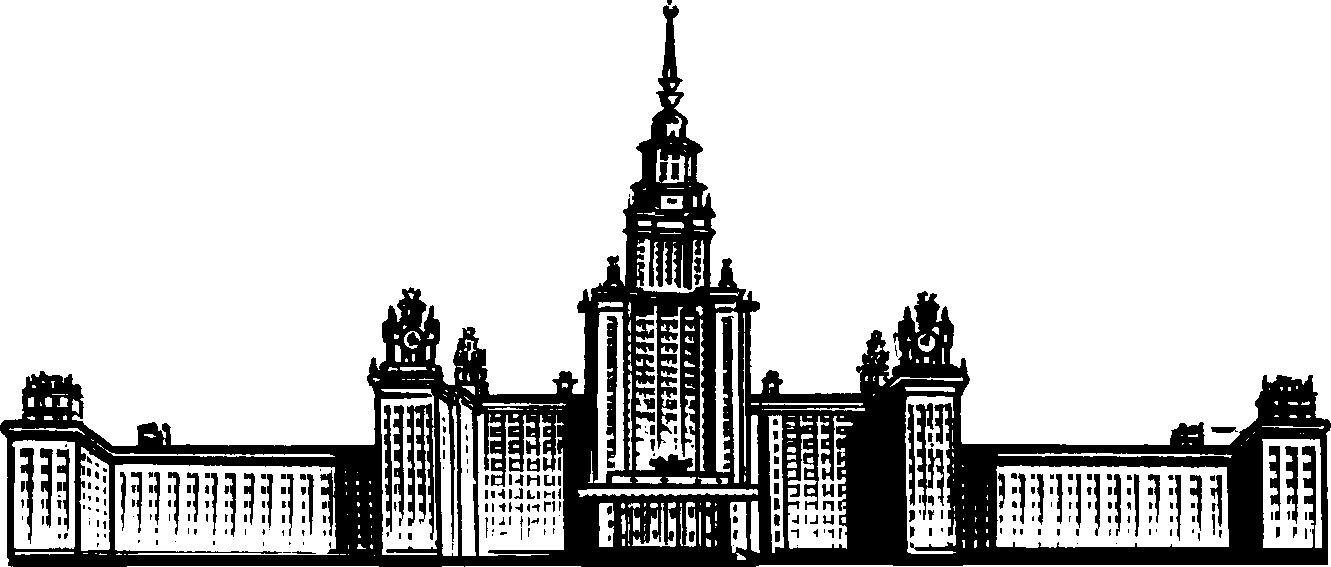
\includegraphics[height=3.5cm]{gzlogo}
\end{center}

 % \begin{minipage}[b]{0.5\linewidth}
  %  \begin{flushright}
      %На правах рукописи\\
%      \textsl {УДК \thesisUdk}
  %  \end{flushright}
 % \end{minipage}
%}{
%\begin{flushright}
%На правах рукописи

%\textsl {УДК \thesisUdk}
%\end{flushright}
%}
%
\vspace{0pt plus6fill} %число перед fill = кратность относительно некоторого расстояния fill, кусками которого заполнены пустые места
\begin{center}
{\large \thesisAuthor}
\end{center}
%
\vspace{0pt plus1fill} %число перед fill = кратность относительно некоторого расстояния fill, кусками которого заполнены пустые места
\begin{center}
\textbf {\large %\MakeUppercase
\thesisTitle}

\vspace{0pt plus2fill} %число перед fill = кратность относительно некоторого расстояния fill, кусками которого заполнены пустые места
{%\small
Специальность \thesisSpecialtyNumber\ "---

<<\thesisSpecialtyTitle>>
}

\ifdefined\thesisSpecialtyTwoNumber
{%\small
Специальность \thesisSpecialtyTwoNumber\ "---

<<\thesisSpecialtyTwoTitle>>
}
\fi

\vspace{0pt plus2fill} %число перед fill = кратность относительно некоторого расстояния fill, кусками которого заполнены пустые места
%Диссертация на соискание учёной степени
НАУЧНО-КВАЛИФИКАЦИОННАЯ РАБОТА

%\thesisDegree
\end{center}
%
\vspace{0pt plus4fill} %число перед fill = кратность относительно некоторого расстояния fill, кусками которого заполнены пустые места
\begin{flushright}
\ifdefined\supervisorTwoFio
Научные руководители:

\supervisorRegalia

\ifdefined\supervisorDead
\framebox{\supervisorFio}
\else
\supervisorFio
\fi

\supervisorTwoRegalia

\ifdefined\supervisorTwoDead
\framebox{\supervisorTwoFio}
\else
\supervisorTwoFio
\fi
\else
Научный руководитель:

\supervisorRegalia

\ifdefined\supervisorDead
\framebox{\supervisorFio}
\else
\supervisorFio
\fi
\fi

\end{flushright}
%
\vspace{0pt plus4fill} %число перед fill = кратность относительно некоторого расстояния fill, кусками которого заполнены пустые места
{\centering\thesisCity\ "--- \thesisYear\par}
           % Титульный лист
\include{Dissertation/contents}        % Оглавление
\ifnumequal{\value{contnumfig}}{1}{}{\counterwithout{figure}{chapter}}
\ifnumequal{\value{contnumtab}}{1}{}{\counterwithout{table}{chapter}}
\chapter*{Введение}                         % Заголовок
\addcontentsline{toc}{chapter}{Введение}    % Добавляем его в оглавление

\newcommand{\actuality}{}
\newcommand{\progress}{}
\newcommand{\aim}{{\textbf\aimTXT}}
\newcommand{\tasks}{\textbf{\tasksTXT}}
\newcommand{\novelty}{\textbf{\noveltyTXT}}
\newcommand{\influence}{\textbf{\influenceTXT}}
\newcommand{\methods}{\textbf{\methodsTXT}}
\newcommand{\defpositions}{\textbf{\defpositionsTXT}}
\newcommand{\reliability}{\textbf{\reliabilityTXT}}
\newcommand{\probation}{\textbf{\probationTXT}}
\newcommand{\contribution}{\textbf{\contributionTXT}}
\newcommand{\publications}{\textbf{\publicationsTXT}}

{\actuality} 
\textbf{Актуальность темы.}
Количественный и качественный анализ физических особенностей потоков тепла и их изменчивости --  одна из основных проблем современных океанологии и климатологии. Существует целый ряд открытых вопросов и проблем при количественной оценке тепловых потоков в процессе взаимодействия океан--атмосфера:
\begin{itemize}
	\item Положение и изменения областей с максимальным взаимодействием;
	\item Области преобладания оттока в атмосферу, перераспределения внутри океана;
	\item Сезонные и межгодовые тренды и колебания. 
\end{itemize}

\noindent
\textbf{Мотивация выбора математической модели}
\begin{itemize}
	\item Для понимания и количественного описания взаимодействия океана и атмосферы существуют различные модели и методы, например, основанные на уравнениях гидро-термодинамики. 
	\item Модель СДУ Ито достаточно проста, поскольку математически задача сводится к определению двух коэффициентов (вектора сноса и матрицы диффузии), зная которые, можно с помощью хорошо разработанного математического аппарата получить количественные оценки поведения изучаемых характеристик, провести их анализ и сделать прогноз с оценкой надежности.
	\item С другой стороны, эта модель достаточно общая, так как она включает в себя как динамические модели со случайным форсингом, так и схемы с разделением процесса на тренды, периодическую и случайную составляющую.
\end{itemize}

%\ifsynopsis
%Этот абзац появляется только в~автореферате.

%\else
%Этот абзац появляется только в~диссертации.
%\fi

% {\progress}
% Этот раздел должен быть отдельным структурным элементом по
% ГОСТ, но он, как правило, включается в описание актуальности
% темы. Нужен он отдельным структурынм элемементом или нет ---
% смотрите другие диссертации вашего совета, скорее всего не нужен.

{\aim} данной работы является стохастическое описание динамики процессов и их взаимодействия с помощью математической модели типа стохастического дифференциального уравнения (СДУ) Ито со случайными коэффициентами сдвига и диффузии, а также использование метода Карунена--Лоэва разложения на ортогональные компоненты.

Для~достижения поставленной цели необходимо было решить следующие {\tasks}:
\begin{enumerate}[beginpenalty=10000] % https://tex.stackexchange.com/a/476052/104425
  \item Исследовать, разработать, вычислить и~т.\:д. и~т.\:п.
  %\item Исследовать, разработать, вычислить и~т.\:д. и~т.\:п.
  %\item Исследовать, разработать, вычислить и~т.\:д. и~т.\:п.
  %\item Исследовать, разработать, вычислить и~т.\:д. и~т.\:п.
\end{enumerate}


{\novelty}
Все результаты, полученные в данной научно-квалификационной
работе, являются новыми.
%\begin{enumerate}[beginpenalty=10000] % https://tex.stackexchange.com/a/476052/104425
	
%\item Впервые \ldots
%  \item Впервые \ldots
%  \item Было выполнено оригинальное исследование \ldots
%\end{enumerate}

{\influence} данной работы заключается в ... TODO

{\methods} В научно-квалификационной работе используются методы математического моделирования, теории вероятностей, математической статистики.

{\defpositions}
\begin{enumerate}[beginpenalty=10000] % https://tex.stackexchange.com/a/476052/104425
  \item TODO
  \item TODO Сравнение методов реконструкции оценок на модельных и реальных данных
  \item TODO Реализация разложения оценок коэффициента диффузии на собственные вектора на основе алгоритма Карунена-Лоэва
  %\item Четвертое положение
\end{enumerate}
%В папке Documents можно ознакомиться с решением совета из Томского~ГУ
%(в~файле \verb+Def_positions.pdf+), где обоснованно даются рекомендации
%по~формулировкам защищаемых положений.

{\reliability} полученных результатов обеспечивается \ldots \ Результаты находятся в соответствии с результатами, полученными другими авторами.


{\probation}
Основные результаты работы докладывались автором
на следующих конференциях:
\begin{enumerate}[beginpenalty=10000]
	\item Осипова А. А., Горшенин А. К., Беляев К. П. Стохастические методы совместного анализа данных температуры воды, потоков тепла и атмосферного давления в Северной Атлантике // Тезисы докладов научной конференции Тихоновские чтения (2024 г., МАКС Пресс, Москва, тезисы). — Т. 46 из Издательский отдел факультета ВМК МГУ имени М.В. Ломоносова. — Москва: ООО МАКС Пресс, 2024. — С. 115.
	\item Осипова А. А., Горшенин А. К. О статистическом оценивании параметров динамико-стохастической модели потоков тепла между океаном и атмосферой // Ломоносовские чтения-2022: научная конференция, факультет ВМК МГУ имени М.В.Ломоносова. Тезисы докладов. — Т. 2022 из СЕКЦИЯ ВЫЧИСЛИТЕЛЬНОЙ МАТЕМАТИКИ И КИБЕРНЕТИКИ. — Москва: ООО МАКС Пресс, 2022. — С. 170–171.
	\item Осипова А. А., Горшенин А. К. Прогнозирование временных рядов на основе гребневой регрессии и расширения признакового пространства // Тихоновские чтения: научная конференция: 25–30 октября 2021 г. : тезисы докладов. — Т. 46. — Москва: ООО МАКС Пресс, 2021. — С. 124–124.
	\item Осипова А. А., Горшенин А. К., Беляев К. П. Совместный анализ температуры воды,
	потоков тепла и атмосферного давления в
	Северной Атлантике // Доклад. Институт океанологии им. П.П. Ширшова Российской академии наук. 27 сентября 2024 года
\end{enumerate}

%{\contribution} Автор принимал активное участие \ldots

\ifnumequal{\value{bibliosel}}{0}
{%%% Встроенная реализация с загрузкой файла через движок bibtex8. (При желании, внутри можно использовать обычные ссылки, наподобие `\cite{vakbib1,vakbib2}`).
    {\publications} Основные результаты по теме диссертации изложены
    в~XX~печатных изданиях,
    X из которых изданы в журналах, рекомендованных ВАК,
    X "--- в тезисах докладов.
}%
{%%% Реализация пакетом biblatex через движок biber
    \begin{refsection}[bl-author, bl-registered]
        % Это refsection=1.
        % Процитированные здесь работы:
        %  * подсчитываются, для автоматического составления фразы "Основные результаты ..."
        %  * попадают в авторскую библиографию, при usefootcite==0 и стиле `\insertbiblioauthor` или `\insertbiblioauthorgrouped`
        %  * нумеруются там в зависимости от порядка команд `\printbibliography` в этом разделе.
        %  * при использовании `\insertbiblioauthorgrouped`, порядок команд `\printbibliography` в нём должен быть тем же (см. biblio/biblatex.tex)
        %
        % Невидимый библиографический список для подсчёта количества публикаций:
        \phantom{\printbibliography[heading=nobibheading, section=1, env=countauthorvak,          keyword=biblioauthorvak]%
        \printbibliography[heading=nobibheading, section=1, env=countauthorwos,          keyword=biblioauthorwos]%
        \printbibliography[heading=nobibheading, section=1, env=countauthorscopus,       keyword=biblioauthorscopus]%
        \printbibliography[heading=nobibheading, section=1, env=countauthorconf,         keyword=biblioauthorconf]%
        \printbibliography[heading=nobibheading, section=1, env=countauthorother,        keyword=biblioauthorother]%
        \printbibliography[heading=nobibheading, section=1, env=countregistered,         keyword=biblioregistered]%
        \printbibliography[heading=nobibheading, section=1, env=countauthorpatent,       keyword=biblioauthorpatent]%
        \printbibliography[heading=nobibheading, section=1, env=countauthorprogram,      keyword=biblioauthorprogram]%
        \printbibliography[heading=nobibheading, section=1, env=countauthor,             keyword=biblioauthor]%
        \printbibliography[heading=nobibheading, section=1, env=countauthorvakscopuswos, filter=vakscopuswos]%
        \printbibliography[heading=nobibheading, section=1, env=countauthorscopuswos,    filter=scopuswos]}%
        %
        \nocite{*}%
        %
        {\publications} Основные результаты по теме диссертации изложены в~\arabic{citeauthor}~печатных изданиях,
        \arabic{citeauthorvak} из которых изданы в журналах, рекомендованных ВАК%
        \ifnum \value{citeauthorscopuswos}>0%
            , \arabic{citeauthorscopuswos} "--- в~периодических научных журналах, индексируемых Web of~Science и Scopus%
        \fi%
        \ifnum \value{citeauthorconf}>0%
            , \arabic{citeauthorconf} "--- в~тезисах докладов.
        \else%
            .
        \fi%
        \ifnum \value{citeregistered}=1%
            \ifnum \value{citeauthorpatent}=1%
                Зарегистрирован \arabic{citeauthorpatent} патент.
            \fi%
            \ifnum \value{citeauthorprogram}=1%
                Зарегистрирована \arabic{citeauthorprogram} программа для ЭВМ.
            \fi%
        \fi%
        \ifnum \value{citeregistered}>1%
            Зарегистрированы\ %
            \ifnum \value{citeauthorpatent}>0%
            \formbytotal{citeauthorpatent}{патент}{}{а}{}%
            \ifnum \value{citeauthorprogram}=0 . \else \ и~\fi%
            \fi%
            \ifnum \value{citeauthorprogram}>0%
            \formbytotal{citeauthorprogram}{программ}{а}{ы}{} для ЭВМ.
            \fi%
        \fi%
        % К публикациям, в которых излагаются основные научные результаты диссертации на соискание учёной
        % степени, в рецензируемых изданиях приравниваются патенты на изобретения, патенты (свидетельства) на
        % полезную модель, патенты на промышленный образец, патенты на селекционные достижения, свидетельства
        % на программу для электронных вычислительных машин, базу данных, топологию интегральных микросхем,
        % зарегистрированные в установленном порядке.(в ред. Постановления Правительства РФ от 21.04.2016 N 335)
    \end{refsection}%
    \begin{refsection}[bl-author, bl-registered]
        % Это refsection=2.
        % Процитированные здесь работы:
        %  * попадают в авторскую библиографию, при usefootcite==0 и стиле `\insertbiblioauthorimportant`.
        %  * ни на что не влияют в противном случае
        \nocite{vakbib2}%vak
        \nocite{patbib1}%patent
        \nocite{progbib1}%program
        \nocite{bib1}%other
        \nocite{confbib1}%conf
    \end{refsection}%
        %
        % Всё, что вне этих двух refsection, это refsection=0,
        %  * для диссертации - это нормальные ссылки, попадающие в обычную библиографию
        %  * для автореферата:
        %     * при usefootcite==0, ссылка корректно сработает только для источника из `external.bib`. Для своих работ --- напечатает "[0]" (и даже Warning не вылезет).
        %     * при usefootcite==1, ссылка сработает нормально. В авторской библиографии будут только процитированные в refsection=0 работы.
}
 % Характеристика работы по структуре во введении и в автореферате не отличается (ГОСТ Р 7.0.11, пункты 5.3.1 и 9.2.1), потому её загружаем из одного и того же внешнего файла, предварительно задав форму выделения некоторым параметрам

\textbf{Объем и структура работы.} Диссертация состоит из~введения,
\formbytotal{totalchapter}{глав}{ы}{}{},
заключения и
\formbytotal{totalappendix}{приложен}{ия}{ий}{}.
%% на случай ошибок оставляю исходный кусок на месте, закомментированным
%Полный объём диссертации составляет  \ref*{TotPages}~страницу
%с~\totalfigures{}~рисунками и~\totaltables{}~таблицами. Список литературы
%содержит \total{citenum}~наименований.
%
Полный объём диссертации составляет
\formbytotal{TotPages}{страниц}{у}{ы}{}, включая
\formbytotal{totalcount@figure}{рисун}{ок}{ка}{ков} и
\formbytotal{totalcount@table}{таблиц}{у}{ы}{}.
Список литературы содержит
\formbytotal{citenum}{наименован}{ие}{ия}{ий}.


%Диссертация организована следующим образом:
% В разделе 2 приведен обзор известных подходов к описанию поведения явного и скрытого потоков тепла, применявшихся за последние 10 лет.
%раздел~\ref{SecModel} содержит описание математической модели, применяющейся в данной работе, а также информацию об анализируемых данных. Раздел~\ref{SecMethods} посвящен вычислительным методам оценивания случайных коэффициентов СДУ Ланжевена. В разделе~\ref{SecSoftware} обсуждается архитектура программного комплекса, реализованного для проведения стохастического анализа потоков тепла с использованием высокопроизводительных вычислительных ресурсов. В разделе~\ref{SecAnalysis} проводится анализ поведения различных характеристик полученных оценок (максимум, минимум, среднее), а также исследуется взаимосвязь между оценками и значениями потоков, на основе которых они были построены. В разделе~\ref{SecDiscuss} обсуждаются полученые результаты и их связь с ранее установленными в данной области эффектами. В Приложении~\ref{AppExist} продемонстирована корректность применения стохастической модели для анализируемых данных. 
    % Введение
\ifnumequal{\value{contnumfig}}{1}{\counterwithout{figure}{chapter}
}{\counterwithin{figure}{chapter}}
\ifnumequal{\value{contnumtab}}{1}{\counterwithout{table}{chapter}
}{\counterwithin{table}{chapter}}
\chapter{Методы реконструкции случайных коэффициентов стохастического дифференциального уравнения Ито}
\label{ch:Methods}

\section{Обзор литературы}
\label{sec:ch1/SecWorks}

На границе между океаном и атмосферой турбулентные тепловые потоки сильно изменяются в различных пространственных и временных масштабах~\cite{small2019air, tian2017air}. Турбулентные потоки вносят значительный вклад в изменчивость общего стока в межгодовом масштабе времени ~\cite{bentamy2017review}.
Также была изучена взаимосвязь между динамикой океана и изменчивостью температуры в смешанном слое в разных регионах~\cite{ashin2019observed, schmeisser2019role}. Теплообмен между океаном и атмосферой тесно связан с температурой поверхности океана, который оказывает значительное влияние на региональный климат. Также известно, что большая часть изменчивости температуры поверхности определяется именно поверхностными тепловыми потоками ~\cite{patrizio2021quantifying}. 
Поведение циклонов и их взаимосвязь с ТПМ и тепловыми потоками, то есть взаимосвязь между приземным атмосферным давлением и тепловыми потоками были рассмотрены в работе ~\cite{tilinina2018association}.

Существует множество работ, посвященных применению методов разложения различных характеристик на ортогональные составляющие в метеорологии, океанологии и климатологии. Можно упомянуть как новаторские исследования ~\cite{lorenz1956empirical, bagrov1959analytic,Obukhov1960,Yudin1968}, так и современные~\cite{kobayashi2015jra}. Оригинальность нашей работы заключается в разработке и применении оригинального метода оценки соответствующих ковариационных матриц большой размерности и их разложения на естественные ортогональные функции с использованием модели СДУ Ито.

Взаимосвязь между аномалиями в явных и скрытых тепловых потоках и значениями SST над районами Северной Атлантики и Северной части Тихого океана была исследована в работе ~\cite{cayan1992latent}. Роль условий преобразования энергии изо дня в день в течение жизненного цикла Североатлантического колебания, которое оказывает существенное влияние на погоду и климат в различных временных масштабах рассматривалась в работе ~\cite{kim2024phase}. Была исследована реакция поверхностного слоя океана на неглубокую конвекцию в атмосфере~\cite{brilouet2024numerical}. Изменчивость в Североатлантическом европейском регионе рассматривалась с использованием модели только для атмосферы, основанной на смещениях SST~\cite{keeley2012impact}. Новизна нашего исследования заключается в изучении пар геофизических величин, таких как тепловые потоки воздуха и моря, атмосферное давление и температура поверхности моря. Мы стремимся выявить взаимосвязи между этими величинами и интерпретировать результаты, используя параметры стохастической модели.


Известно, что на поверхности раздела двух сред -- океана и атмосферы -- турбулентные потоки тепла имеют высокую волатильность на различных пространственно-временных масштабах (\cite{small2019air}, \cite{tilinina2018association}, \cite{tian2017air}). В работе \cite{bentamy2017review} для данных реанализа было продемонстрировано, что именно турбулентные потоки вносят основной вклад в изменчивость общего потока на межгодовом масштабе времени. Связь динамики океана и изменчивости температуры смешанного слоя в различных регионах изучается в целом ряде работ~\cite{ashin2019observed,schmeisser2019role,patrizio2021quantifying}.
% 	В работе \cite{patrizio2021quantifying} было показано, что динамический вклад океана в дисперсию температуры смешанного слоя имеет наибольшие значения в областях западных пограничных течений.
% 	, их продолжениями на восток и областями экваториального апвеллинга.
% 	Авторы также показывают, что динамика океана уменьшает дисперсию температур смешанного слоя в северном полушарии при рассмотрении во временных масштабах более нескольких лет, в результате чего утверждается, что в среднем по миру относительный вклад динамики океана в изменчивость температуры смешанного слоя уменьшается на все более низких частотах.
% 	Связь динамики океана и изменчивости температуры смешанного слоя в различных регионах изучается в целом ряде работе~\cite{ashin2019observed,schmeisser2019role,patrizio2021quantifying} лась в работе~\cite{schmeisser2019role}, где рассматриваются причины возникновения аномально выхоких поверхностных температур в период 2013-2015гг. в Северо-Восточной части Тихого океана, а также в статье \cite{}, где рассматривается их межсезонная и внутрисезонная изменчивость в области Андаманского моря. 
Потоки тепла между океаном и атмосферой тесно связаны с величиной SST (Sea Surface Temperature) -- температурой поверхности океана, оказывающей влияние на региональный климат. Известно, что большая часть изменчивости SST определяется именно рассматриваемыми поверхностными тепловыми потоками~\cite{schneider2015atmospheric,hausmann2017mechanisms,li2019decadal,blein2022parametrizing}. Существует целый ряд вопросов и проблем при количественной оценке тепловых потоков в процессе взаимодействия океана и атмосферы. Важно понять, где локально и как изменяются те области, в которых происходит максимальное взаимодействие, где количественно больше идет отток в атмосферу или наоборот поступление тепла и влаги из атмосферы, а где тепло больше перераспределяется внутри океана. Как это меняется по сезонам? Есть ли межгодовые тренды и колебания? Все эти вопросы окончательных ответов не имеют и более того, даже их постановка не кажется корректной в отсутствии адекватных моделей описания процессов взаимодействия.
% изучается десятилетняя изменчивость SST в юго-восточной части Индийского океана и ее влияние на
% региональный климат, причем показано, что большая часть изменчивости SST определяется именно рассматриваемыми поверхностными тепловыми потоками. Авторы статьи~\cite{hausmann2017mechanisms} показывают, что обратная связь турбулентного теплового потока между океаном и атмосферой является основным фактором, влияющим на настройку демпфирования временной шкалы аномалий температуры поверхности моря. Работа~\cite{schneider2015atmospheric} посвящена реакции атмосферы на слабые фронты температуры поверхности моря. В статье~\cite{blein2022parametrizing} изучается мезомасштабное усиление приземных турбулентных потоков на границе раздела воздух-море. В частности, декларируется, что оно обусловлено мезомасштабной изменчивостью скорости приземного ветра, особенно скоростью порывов ветра и мезомасштабными стандартными вариациями скорости ветра. В этом исследовании предлагается параметризация этих двух переменных.

Вероятностные результаты в данной области касаются аппроксимации распределения данных потоков тепла двухпараметрическим распределением Фишера--Триппета с оценкой его параметров по данным базы реанализа NCEP--NCAR за период 1948-2008 гг.~\cite{gulev2012probability}. В статье~\cite{FAO} изучено статистическое поведение экстремальных характеристик потоков (максимум, минимум) по области за весь период наблюдений в точках одноградусной сетки при различных осреднениях от суточных до годовых, а также средних значений по распределению и медиан. Кроме того, проведена аппроксимация вероятностных распределений для каждого из типов потоков тепла по отдельности и исследованы их совместные распределения.

Наиболее часто для анализа используются данные различных баз реанализа, содержащие аппроксимации реальных наблюдений~\cite{cronin2019air,leyba2019trends} на основе некоторых характерных значений для контактных сред. В данной статье в качестве данных для стохастической аппроксимации выступают элементы открытой базы реанализа ERA5\footnote{https://www.ecmwf.int/en/forecasts/datasets/reanalysis-datasets/era5}, формируемой Европейским центром среднесрочных прогнозов погоды.

Для изучения динамики процессов с учетом случайных факторов традиционным инструментом является аппарат случайных процессов. В физике плазмы~\cite{Espinos2018,Sexty2019} и финансовой математике~\cite{Bouchaud1998} хорошо известно стохастическое дифференциальное уравнение (СДУ) Ито (см. формулу~\eqref{Ito} далее). Однако в области климатологии модели на его основе используются лишь в небольшом количестве работ для описания процессов, протекающих в океане. В частности, см., например, статьи~\cite{van2021characterisation,toppaladoddi2021stochastic}, где в которых СДУ Ито используется для описания поведения потоков тепла между льдом и океаном в области Арктики.

% сформулирована гипотеза о том, что  В работе~\cite{FAO} на данных явных и скрытых потоков тепла в области Северной Атлантики из базы ERA-5 подробно исследуются статистические закономерности внутригодовой и межгодовой изменчивости с различными масштабами усреднения: дневным, месячным, годовым. Рассмотрено поведение экстремальных и средних потоков: в частности, показано существование положительного тренда максимума скрытого потока с течением времени.

% В данной работе не рассматриваются особенности измерения и алгоритмов приближения этих величин, данные реанализа этих величин были взяты из открытой базы ERA-5 и считаются известными безотносительно способа их получения. Фокус внимания данной работы состоит в оценивании и исследовании поведения случайных величин в математической модели стохастического дифференциального уравнения (СДУ) Ито~\ref{Ito}, в котором участвуют значения потоков тепла как значения случайного процесса.

% Данная статья продолжает и обобщает идею статьи \cite{Belyaev2021} по применению модели уравнения Ланжевена для описания потоков тепла между океаном и атмосферой. Приводится алгоритм оценки параметров данной модели и затем применяется для получения оценок с использованием данных из базы ERA-5 о потоках тепла в области Северной Атлантики. Кроме того, проводится исследование поведения полученных оценок с течением времени, рассматривается их взаимодействие и эффект преобладания диффузиозной компоненты над параметром сноса.

Первые исследования среднегодового хода явных потоков тепла по данным реанализа базы ERA5 за $2010$--$2020$~гг. с использованием СДУ Ито были проведены авторами данного исследования в статье~\cite{Belyaev2021}. В ней были изучены статистические закономерности внутригодовой и межгодовой изменчивости с различными масштабами усреднения: дневным, месячным, годовым. Также рассматривалось поведение экстремальных и средних потоков. В частности, показано существование положительного тренда максимума скрытого потока с течением времени. 

В данной статье анализируются как явные, так и скрытые потоки, в том числе и совместно, на значительно более длинном временном интервале $1979$--$2022$~гг. Предложены оригинальные методы оценивания векторного коэффициента сноса $a$ и матричного коэффициента $b$ СДУ Ланжевена, исследуется взаимовлияние этих величин, выявляются области преобладания диффузиозной компоненты над параметром сноса, а также рассматривается поведение таких их характеристик, как минимумы, максимумы и средние значения.
% Кроме того, проверяется выполнение условия корректности применения предлагаемой математической модели для подобного рода данных. 
Ориентированность на анализ этих величин связана с их физическим смыслом. Так, коэффициент сноса показывает преимущественное направление потоков внутри океана, а коэффициент диффузии позволяет выявить области основного обмена теплом океана с атмосферой. Кроме того, он важен при оценках теплобаланса.

Статья организована следующим образом:
% В разделе 2 приведен обзор известных подходов к описанию поведения явного и скрытого потоков тепла, применявшихся за последние 10 лет.
раздел~\ref{SecModel} содержит описание математической модели, применяющейся в данной работе, а также информацию об анализируемых данных. Раздел~\ref{SecMethods} посвящен вычислительным методам оценивания случайных коэффициентов СДУ Ланжевена. В разделе~\ref{SecSoftware} обсуждается архитектура программного комплекса, реализованного для проведения стохастического анализа потоков тепла с использованием высокопроизводительных вычислительных ресурсов. В разделе~\ref{SecAnalysis} проводится анализ поведения различных характеристик полученных оценок (максимум, минимум, среднее), а также исследуется взаимосвязь между оценками и значениями потоков, на основе которых они были построены. В разделе~\ref{SecDiscuss} обсуждаются полученые результаты и их связь с ранее установленными в данной области эффектами. В Приложении~\ref{AppExist} продемонстирована корректность применения стохастической модели для анализируемых данных. 


Одной из главных задач современной метеорологии, океанографии и климатологии является понимание того, как взаимодействуют тепловые потоки, температура поверхности моря и приземное атмосферное давление. Анализируя изменчивость и физические характеристики тепловых потоков и их взаимосвязь с другими метеорологическими переменными, такими как SST и давление на уровне моря, можно получить ценную информацию о климатической системе Земли. Эти знания имеют решающее значение для улучшения средне- и долгосрочного прогнозирования погоды. Это позволяет более точно прогнозировать опасные явления, такие как тропические ураганы, цунами и другие опасные явления. Кроме того, это помогает понять антропогенное воздействие на окружающую среду и различные другие факторы, влияющие на климат нашей планеты.



При построении количественных оценок тепловых потоков в системе океан-атмосфера большой интерес представляют вопросы о зонах со значительным взаимодействием и соответствующих местных характеристиках, а также о сезонных эффектах и межгодовых тенденциях и колебаниях.
\begin{itemize}
	\item Как меняются области, где происходит наиболее значимое взаимодействие, и каковы локальные характеристики этих областей?
	\item Где происходит количественный отток в атмосферу или, наоборот, поступление тепла и влаги из атмосферы, и где тепло в большей степени перераспределяется внутри океана?
	\item Как эти эффекты меняются в зависимости от времени года?
	\item Существуют ли межгодовые тенденции и колебания? Как изменения в тепловых потоках, температуре поверхности моря и атмосферном давлении проявляются количественно в различных масштабах пространства и времени?
	\item Существуют ли какие-либо изолированные океанские структуры, такие как квазициклонические или антициклонические вихри, где эти процессы взаимодействия можно в какой-то степени считать стационарными?
\end{itemize}
На эти вопросы нет однозначных ответов, и, более того, даже их формулировка может быть некорректной без адекватных математических моделей для описания процессов взаимодействия.
Такие вопросы рассматриваются и решаются в численных гидродинамических моделях, которые моделируют взаимодействие океана и атмосферы~\cite{gulev2012probability}.
Однако эти модели в значительной степени зависят от трудно поддающихся оценке внешних и внутренних факторов: коэффициентов вязкости, уровней турбулентности и скоростей обмена. Эти факторы либо неизвестны, либо их трудно определить на основе наблюдений. Кроме того, существует зависимость от начальных и граничных условий, которые также сложно определить. Некоторые компромиссы основаны на моделях, которые включают в себя ассимиляцию данных~\cite{FAO}. Однако, даже в случаях усвоения данных расчеты для долгосрочных периодов требуют установки дополнительных параметров.

Вероятностные и статистические модели, основанные исключительно на наблюдениях, могут быть более эффективными для долгосрочного моделирования и прогнозирования.
Распределения этих тепловых потоков могут быть аппроксимированы двухпараметрическим распределением Фишера-Типпета ~\cite{gulev2012probability}.
Ранее было изучено статистическое поведение экстремальных характеристик потока (максимум, минимум) в Североатлантическом регионе за весь период наблюдений в точках одноградусной сетки при различных средних масштабах от суточного до годового, а также распределения вероятностей для каждого типа тепловых потоков~\cite{FAO}.
Кроме того, были аппроксимированы распределения вероятностей для каждого типа тепловых потоков по отдельности и исследованы их совместные распределения.
Однако нет результатов для совместных распределений SST, потоков и давления, хотя все эти значения физически и статистически зависимы.

Мы расширяем математическую базу, представленную в наших предыдущих работах ~\cite{Belyaev2021,FAO, Gorshenin2023}, для изучения динамики процессов под воздействием случайных факторов, основываясь на стохастических дифференциальных уравнениях (СДУ)~\cite{Skorohod}. Хотя эти аспекты известны, они используются лишь в ограниченном числе исследований в области океанологии и метеорологии для описания процессов, происходящих в океане. Чаще всего для вероятностного анализа используются данные из различных баз данных реанализа, которые содержат приближения к реальным наблюдениям, основанные на определенных характеристиках контактирующих поверхностей.
Мы используем базу данных реанализа ERA5~\cite{hersbach2020era5}, созданную Европейским центром среднесрочных прогнозов погоды.

В работе ~\cite{van2021characterisation} были проведены исследования изменчивости явных и скрытых потоков, их экстремальных и средних значений в внутри- и межгодовом масштабе на основе данных из базы данных ERA5. Совместное поведение явных и скрытых потоков, их тренды и ковариационные функции в различных пространственно-временных масштабах изучались в работе ~\cite{toppaladoddi2021stochastic}.

Фундаментальная новизна нашего исследования по сравнению с предыдущими исследованиями в этой области (см., например, статьи~\cite{van2021 characterization,toppaladoddi2021stochastic}, а также раздел ~\ref{SecWorks}) заключается в том, что мы исследуем совместное распределение трех ключевых характеристик: температуры поверхности океана, суммарного теплового потока и приземного атмосферного давления.
Кроме того, мы используем метод Карунена-Лоэва, чтобы разложить эти величины на собственные векторы (ортогональные компоненты), обеспечивая более глубокое понимание лежащих в их основе закономерностей и взаимосвязей.

Представленные методы также используются для оценки векторного коэффициента дрейфа, а также матрицы диффузии в СДЕ Ито, при этом как коэффициент дрейфа, так и матрица диффузии зависят от времени и от всего вектора наблюдений (подробности см. в статьях ~\cite{Gorshenin2023,belyaev2024comparison}.





В системе океан–атмосфера поведение теплового потока и изменчивость каждого компонента играют важную роль, поскольку они оказывают значительное влияние \cite{perry1977ocean} на климатические особенности этой системы, что делает их количественный и качественный анализ одной из основных проблем современной океанологии и климатологии. Распределение явных и скрытых тепловых потоков было ранее исследовано и аппроксимировано с использованием двухпараметрического распределения Фишера-Типпетта.
В данной работе в качестве модели динамики изменчивости теплового потока в системе воздух-море используется хорошо известное стохастическое дифференциальное уравнение Ито (SDE) \cite{Pascucci2022}. Задача оценки (вообще говоря) случайных коэффициентов SDE, учитывая наблюдения за процессом, предполагает некоторые существенные допущения относительно математических свойств коэффициентов \cite{Yoshida1992, GenonCatalot1993, GenonCatalot1994, Wei2016}. В работах \cite{Yoshida1992, GenonCatalot1993, GenonCatalot1994, Wei2016} авторы предполагают, что коэффициенты являются функциями неизвестного параметра $\theta$; некоторые из них даже предполагают определенный тип зависимости от этого параметра. В работе \cite{FlorensZmirou1993} рассмотрен непараметрический случай, и оценка коэффициента диффузии, наряду с доказательством его сходимости и непротиворечивости, получена в предположении существования трех непрерывных ограниченных производных этого коэффициента, а также неслучайности и существования ограниченных производных коэффициента дрейфа. Также можно использовать основанный на ядре метод регрессии \cite{Lamouroux2009}.
Применение модели Ито для оценки эволюции приращения теплового потока было ранее рассмотрено в работе \cite{Belyaev2021}. Модель СДУ Ито обобщает хорошо известные статистические модели динамики климата, в частности, модели Будыко \cite{Budyko1974} и Хассельмана \cite{Hasselmann1976}. Эта модель также представлена в работах \cite{van2021characterisation, toppaladoddi2021stochastic}, где авторы использовали ее для описания поведения тепловых потоков между льдом и океаном в Арктическом регионе. Статистические особенности модели в двумерном случае были подробно рассмотрены в \cite{Pascucci2022}. Оценка неизвестного параметра модели в многомерном случае уравнения Ланжевена, являющегося вариантом уравнения Ито, была предложена в работе \cite{Voutilainen2022}.
Параметр дрейфа в уравнении Ито соответствует средним изменениям в поведении системы с течением времени, зависящим как от конкретного момента времени, так и от величины потока. Выявление областей, где этот коэффициент является значительным, может быть полезно для определения зон струйных течений, фронтов и синоптических вихрей, где происходят значительные динамические процессы. Области с малым коэффициентом дрейфа и большим стохастическим (диффузионным) коэффициентом соответствуют областям сильной турбулентности, включая энергетически активные области в Северной Атлантике. Поэтому задача оценки параметров стохастической модели поведения приращения тепловых потоков важна для решения задач с точки зрения математического моделирования.
Моделирование приращений потоков (в отличие от традиционно используемого для изучения значений самих потоков) адекватно описывает динамику потоков в среднесрочной и долгосрочной перспективе и, по-видимому, хорошо согласуется с реальными данными. Эта модель имеет ряд преимуществ перед известными численными или стохастическими моделями. Она довольно проста, поскольку форма модели определяется двумя коэффициентами, даже в многомерном случае (вектор дрейфа и матрица диффузии). Таким образом, можно количественно оценить поведение изучаемых характеристик, т.е. проанализировать и спрогнозировать их. Кроме того, эта схема является довольно общей, поскольку она включает как динамические модели со случайным воздействием (т.е. внешним воздействием), так и модели, основанные на тенденциях в периодических и случайных компонентах. Чтобы проверить адекватность модели, авторы ранее рассмотрели статистические закономерности внутри- и межгодовой изменчивости явных и скрытых тепловых потоков в Северной Атлантике, используя временные ряды из базы данных повторного анализа ERA5 \cite{Belyaev2022}. Было изучено поведение максимумов, минимумов, средних и медианных значений по рассматриваемой акватории с течением времени. Было показано, что в динамике скрытого теплового потока наблюдается положительная тенденция, и были оценены его параметры. Предлагаемая модель использует хорошо развитый аппарат теории стохастических дифференциальных уравнений и параболических уравнений Фоккера-Планка–Колмогорова, поэтому она удобна, например, для количественных и качественных оценок динамики потоков, их пространственно–временной изменчивости и вероятностей возникновения редких, но опасных событий., тропические ураганы.
Как было отмечено выше, непараметрический метод имеет строгие теоретические обоснования, однако он требует выполнения некоторого набора условий для коэффициентов, которые часто не могут быть проверены на реальных геофизических данных. Альтернативным рассматриваемым подходом является полупараметрический статистический метод, основанный на восстановлении распределений неизвестных коэффициентов случайного дрейфа и диффузии SDE, который подразумевает, что процесс оценки выполняется с использованием набора смесей нормалей произвольного масштаба сдвига. Стоит отметить, что в случае неслучайных коэффициентов рассматриваемого SDE, при принятии дополнительных предположений об измеримости в отношении естественной фильтрации и нормальности распределения начального значения процесса, решением оказывается некоторый гауссовский процесс с заданным средним значением и ковариационной функцией. Строгая теоретическая постановка задачи сходимости для полупараметрического метода сложна; этот вопрос обсуждается ниже в этой статье (см. раздел 3.3). Поэтому в данной статье полупараметрический подход, свободный от каких-либо дополнительных допущений, сравнивается с непараметрическим, чтобы продемонстрировать близость результатов и, как следствие, корректность его применения. Одно из важных потенциальных применений полупараметрического метода связано с задачей прогнозирования. В его рамках возникают теоретически обоснованные аппроксимации распределений для решений SDE. Эти распределения, или, скорее, параметры и компоненты связности, полученные в результате их оценки, могут быть использованы в рамках машинного обучения, основанного на физике (ML). Некоторые примеры эффективного улучшения прогнозов нейронной сети с использованием этого метода были продемонстрированы ранее в \cite{Kuzmin2022} для нескольких тепловых потоков в Лабрадорском море и Гольфстриме. Стоит отметить, что для получения точечных оценок с помощью первого подхода в данном случае может потребоваться решение нескольких задач SDE.

\section{Математическая модель}
\label{SecModel}
В работе изучаются данные реанализа базы ERA5 явного и скрытого потоков тепла в Северной Атлантике за период с $1$ января $1979$ года по $30$ сентября $2022$ года.
Данные сосредоточены в узлах равномерной сетки с шагом в $0.5$ градуса, покрывающей область Северной Атлантики. Границы сетки по широте составляют от $-90$ до $0$ градусов, а по долготе -- от $0$ до $80$ градусов. Шаг измерений по времени составляет $6$ часов, на одни сутки приходится $4$ измерения: в полночь, $06:00$, $12:00$ и $18:00$.

На рисунке~\ref{fig_flux_example} представлен пример визуализации данных с суточным усреднением: график слева соответствует явным, а справа -- скрытым потокам тепла. Цветовая шкала меняется от синего (при отрицательных значениях потоков) до белого (при значениях, близких к нулю) и далее до красного (при положительных значениях). Яркость цвета в конкретной точке соответствует удаленности значения от нуля. Темно-зеленым цветом обозначены участки суши.

\begin{figure}[!h]
	\centering
	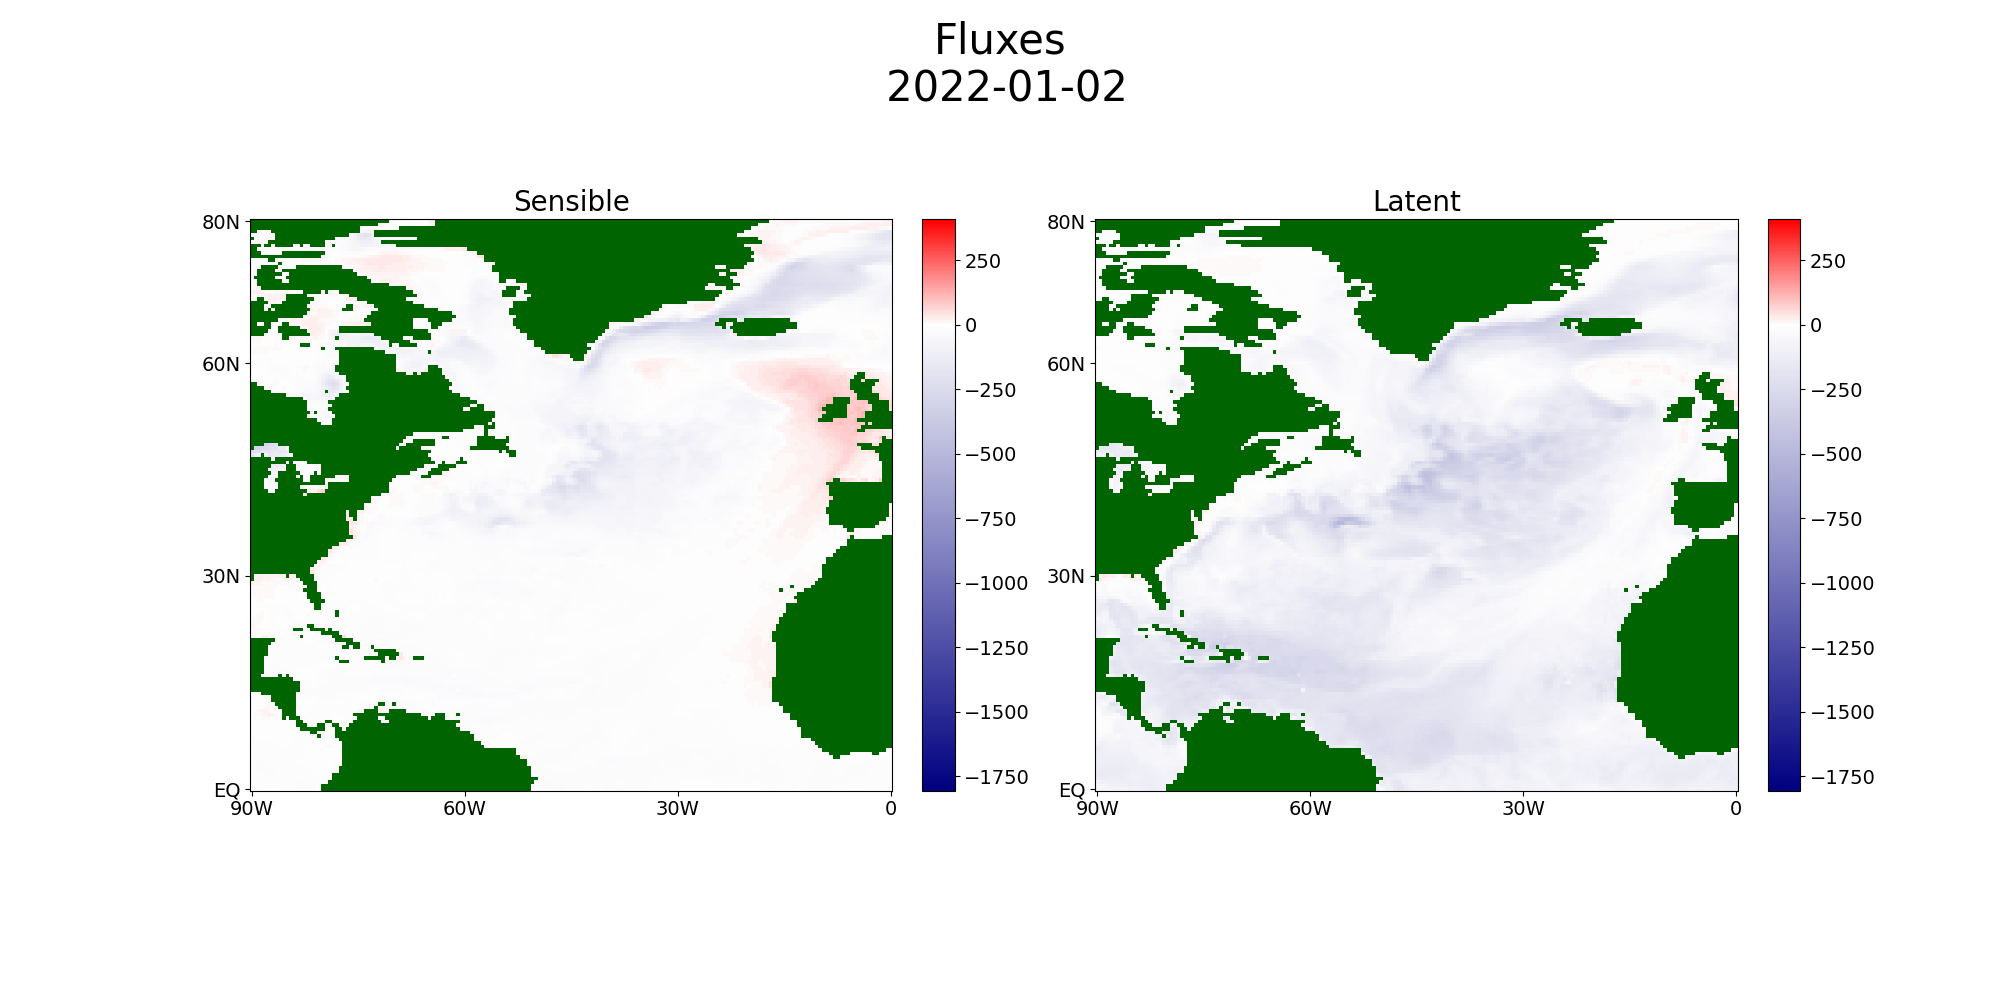
\includegraphics[width=\textwidth]{Flux_00002}
	\caption{Пример визуализация данных по акватории Северной Атлантики с суточным усреднением: слева -- явные, справа -- скрытые потоки}
	\label{fig_flux_example}
\end{figure}

Рассмотрим динамико-стохастическую модель вида
\begin{equation}
	\label{Ito}
	dX = a(t,X)\,dt + b(t, X)\,dW(t), 
\end{equation}
называемую стохастическим дифференциальным уравнением Ито.

Модель~\eqref{Ito} используется для описания случайных процессов диффузионного типа, в которых изменчивость самого процесса за малый промежуток времени мала по сравнению с изменчивостью его среднего значения и дисперсии~\cite{jin2020controls,van2021characterisation}. В таком случае за указанный малый промежуток времени эта изменчивость может рассматриваться как сумма квази-детерминированного процесса, определяемого сносом $a(t, X)$ (здесь термин <<квази>> учитывает наличие зависимости непосредственно от случайного процесса $X$), и чисто случайного процесса $b(t, X)$, не зависящего от первого слагаемого и определяемого диффузионной составляющей.

В формуле~\eqref{Ito} $X = (X_1(t), X_2(t))$ -- случайный процесс, значения которого в фиксированный момент времени $t$ имеют смысл вектора значений явного и скрытого потока в рассматриваемой географической точке, $a(t,X)$ и $b(t,X)$ –- случайные коэффициенты сноса и диффузии, зависящие от времени и значения потока, $dW(t)$ -- винеровский процесс, не зависящий от процесса $X$. Первая компонента векторного коэффициента переноса $a(t, X)=(a_1(t,X), a_2(t,X))$ соответствует явному, а вторая -- скрытому потоку. Для определения коэффициента $b$ рассмотрим оператор диффузии $B(t, x)$ с собственными значениями $\lambda_i(t, x), i=1,2$ и соответствующими собственными векторами $e_i(t, x), i=1,2$. Положим
\begin{equation}
	\label{b_vector}
	b_i(t,x) = \sqrt{\lambda_i(t, x)}e_i(t, x), \quad i=1,2,
\end{equation}
и объединим эти два вектора в матрицу. Коэффициентом $b(t, X)$ будем называть матрицу $2\times2$ со случайными значениями:
\begin{equation}
	\label{eq:b_coeff}
	b(t,X) =  \begin{bmatrix}  
		b_{11}(t, X) & b_{12}(t, X) \\
		b_{21}(t, X) & b_{22}(t, X)
	\end{bmatrix}
\end{equation}
Здесь $b_{ii}(t, X)$ -- соответственно диффузионные компоненты явного и скрытого потоков, а $b_{12}(t,X)$ и $b_{21}(t,X)$ описывают взаимодействие потоков, представляя собой в некотором смысле аналог ковариации. Однако, вообще говоря, $b_{12} \neq b_{21}$.

Решение СДУ \eqref{Ito} представляет собой диффузионный процесс с коэффициентом диффузии $b^2(t, X)$ и коэффициентом дрейфа $a(t,X)$. Случайные коэффициенты $a(t,X)$ и $b^2(t,X)$ представляют собой условное математическое ожидание и дисперсию приращений потока соответственно:
\begin{equation}
	\label{eq:a_coeff_E}
	a(t,X)= \frac{\E(X(t+dt)-X(t)|X(t)=x)}{dt},
\end{equation}
\begin{equation}
	\label{eq:b_coeff_D}
	b^2(t,X)= \frac{\D(X(t+dt)-X(t)|X(t)=x)}{dt},
\end{equation}
где E и D - математическое ожидание и дисперсия случайной величины соответственно.

Для существования решения уравнения~\eqref{Ito} необходимо выполнение некоторых условий~\cite{Skorohod} на рассматриваемые борелевские функции $a(t, x)$ и $b_i(t, x), i=1,2$. В разделе~\ref{AppExist} проведена проверка справедливости этих условий для изучаемых данных реанализа с целью обоснования корректности применения математической модели. Можно продемонстрировать, что для этих данных выполняются условия существования решения СДУ (см. книгу~\cite{Skorohod}, стр. 469). %Почему убрали про однозначное определение свойств временного ряда? Мне кажется, здесь было бы уместно

При отсутствии априорной информации о физической структуре процесса $X(t)$ проблема статистического восстановления функций $a(t)$ и $b(t)$ становится одной из важнейших. Из-за их случайной природы эта задача допускает, по крайней мере, два принципиально различных подхода к ее постановке. Первый из них заключается в получении оценок (которые сами по себе были бы случайными) функций $a(t)$ и $b(t)$, то есть в построении их точечных приближений. Второй подход представляет собой статистическую реконструкцию случайных коэффициентов $a(t)$ и $b(t)$ в терминах их распределений. То есть, зная некоторые свойства этих коэффициентов, можно найти оценки некоторых числовых параметров этих моделей. Оба подхода можно интерпретировать как физически реалистичные и осуществимые.

\section{Непараметрический метод оценивания}
\label{SecNonparametic}
Ключевым предположением при изучении рассматриваемых данных реанализа является предположение, что все их статистические характеристики зависят только от самих значений и не зависят от точки локализации. Иными словами, это допущение того, что значения потока, взятые в разных точках пространства, можно считать принадлежащими одной и той же генеральной совокупности с присущей ей некоторыми статистическими характеристиками. Это предположение вполне обосновано, так как традиционные расчетные формулы для потоков~\cite{cronin2019air,leyba2019trends} используют только сами значения контактных сред, но не их локацию. Поэтому при достаточно больших размерах рассматриваемой области для каждого интервала значений потоков тепла, от минимального до максимального значения потоков в фиксированную дату, найдется достаточно много пространственных точек, и соответственно значений потоков, чтобы оценка вероятности перехода значений потока из одного состояния в другое за небольшой отрезок времени была состоятельна.


\subsection{Дискретизация данных}
\label{Disctretization}
Данные представляются в виде вариационного ряда в фиксированные моменты времени: все значения исследуемой величины потока разбиваются на некоторое количество равных интервалов от минимального до максимального значений и внутри каждой ячейки, независимо от пространственной локализации, проводится их осреднение по пространству. Как было отмечено во Введении, для получения данных реанализа используются только сами значения контактных сред, но не их местоположение. Поэтому при достаточно больших размерах рассматриваемой области для каждого интервала значений потоков тепла от минимального до максимального значения в фиксированную дату найдется достаточно много пространственных точек и, соответственно, значений потоков, чтобы оценка вероятности перехода значений потока из одного состояния в другое за небольшой отрезок времени была состоятельна. Подобный прием хорошо известен в анализе временных рядов, однако для анализа потоков тепла он впервые применен именно коллективом авторов статьи, и в этом смысле является оригинальным. Это позволяет представить временные ряды потоков тепла в виде реализации случайного процесса, описываемого СДУ Ито, и оценить его параметры.

\subsection{Формулы}
Для каждого фиксированного момента времени $t$ точечные оценки $a(t,x)$ и $b(t,x)$ могут быть построены только на основе значения потока.
% -- для этого достаточно определить вероятности перехода процесса из одного состояния в другое. То есть 
Для построения оценок в момент времени $t+1$ требуется на основе выборки по всей рассматриваемой географической области оценить вероятности перехода процесса $X(t)$ из множества значений в момент $t$ в множество значений в момент $t+1$. Будем обозначать значения процесса с помощью строчных букв.

В случае дискретных значений процесса рассмотрим условную вероятность
$\P(y|x) = \P(X(t+dt)=y|X(t)=x)$, а в абсолютно-непрерывном случае -- плотность
$p(y|x)dx = p(y<X(t)|x < X(t) = x)$.
Тогда коэффициенты $a(t, x)$ и $b(t, x)$ для некоторых фиксированных значений двух потоков %$X(t) = (X_1(t), X_2(t))$
$x = (x_1, x_2)$ %и $y = (y_1, y_2)$
определяются \cite{Skorohod} формулами
\begin{gather}
	\label{eq:a_formula_0}
	a_i(t,x_i) = \lim_{\varDelta t \to 0} \frac{1}{\varDelta t} \int\limits_{t}^{t+\varDelta t} (y_i-x_i)p(y_i|x_i)\,dy, \quad i = 1,2;\\
	\label{eq:b_formula_0}
	b_{i, j}^2(t, {x}) = \lim_{\varDelta t \to 0} \frac{1}{\varDelta t} \int\limits_{t}^{t+\varDelta t} (y_i-x_j)(y_i-x_j)^T p(y|x)\,dy, \quad i,j = 1,2.
\end{gather}

Таким образом, для оценки коэффициентов $a(t,x)$ и $b(t,x)$ необходимо оценить переходные вероятности, фигурирующие в правой части формул~\eqref{a_formula_0}--\eqref{b_formula_0} под знаком интеграла. На практике рассматривается процесс с дискретным временем, измерения которого проводятся через фиксированный промежуток времени $\varDelta t$, поэтому предел в правой части равенств~\eqref{a_formula_0}--\eqref{b_formula_0} исчезает, кроме того, с учетом конечности выборки измерений процесса, интегралы заменяются на конечные суммы.

Рассмотрим два соседних момента времени $t_1$ и $t_2$. Для того, чтобы оценить коэффициенты $a(t,x)$ и $b(t,x)$ по формулам~\eqref{a_formula_0}--\eqref{b_formula_0}, потребуется определить значения переходных вероятностей потока с использованием только множества значений в эти соседние моменты времени, поскольку не предполагается однородность процесса. Но в таком случае, учитывая вещественность значений, при фиксации значения $x$ в момент времени $t_1$ ему будет соответствовать, скорее всего, лишь одна географическая точка сетки, в которой достигается это значение. В таком случае соответствующее значение $y$ в момент времени $t_2$ будет единственным отвечающим состоянием с вероятностью перехода, равной $1$, что нельзя считать адекватной оценкой для описания переходов процесса. Поэтому необходимо разбить весь диапазон значений процесса в выборке на непересекающиеся интервалы и заменить все значения, попадающие в этот интервал, на общее значение. Наиболее естественным способом для этого является использование квантилей для построения интервалов с одинаковыми вероятностями попадания в них, с учетом описанного выше предположения локальной однородности данных.

Итак, для каждого типа потока отдельно за некоторый период времени рассматриваются все значения потока. Выбирая $1000$ чисел $\left\lbrace p_1, \ldots, p_{1000} \right\rbrace $, разделяющих  отрезок $[0, 1]$ на части одинаковой длины, для каждого $p_i$ найдем квантиль соответствующего порядка $q_i$, $i=1, \ldots, 1000$. Затем каждое значение потока, попавшее в интервал $[q_i, q_{i+1}]$, заменяется величиной $(q_i + q_{i+1})/2$. В некотором смысле это похоже на процесс приближения абсолютно-непрерывной случайной величины с помощью дискретной.

Обозначим полученное множество возможных значений процесса как $X_1, X_2, \dots, X_{1000}$, где $X_i = (q_i + q_{i+1})/2$. Далее для каждого $t \in [0, T-1]$ оценим вероятности перехода процесса из одного состояния в другое:
\begin{equation}
	\label{p_formula}
	p_{ij} = \frac{\#\{X(t) = X_i, X(t+1) = X_j\}}{\#\{X(t) = X_i\},}
\end{equation}
где символ $\#$ обозначает количество элементов в соответствующем множестве, $j = 1,\ldots,1000$, $i \in \{1, \dots, 1000\}: \#\{X(t) = X_i\} > 0$. Очевидно, что при этом для $i$, соответствующих непустому набору в момент времени $t$, $\sum\limits_{j=1}^{1000} p_{ij} = 1$. Эту процедуру можно выполнить как рассматривая один тип потока в оба момента времени, так и разные типы потоков, получая $4$ набора вероятностей: для пары явный поток-явный поток, явный поток-скрытый поток, скрытый поток-явный поток и скрытый поток-скрытый поток. Обозначим эти наборы, соотвественно, $P_{sens-sens}, P_{sens-lat}, P_{lat-sens}, P_{lat-lat}$. 

Оценки для коэффициента переноса $a(t,x)$ в момент времени $t \in [0, T-1]$ в точках, соответствующих значению потока (явного или скрытого для разных компонент отвечающего вектора) $x_i \in \{X_1, \dots, X_{1000}\}$, строятся следующим образом:  
\begin{equation}
	\label{a_formula}
	a_{x_i} = \sum\limits_{j=1}^{1000} (x_i - y)\cdot p_{ij}, \quad x_i, y \in \{X_1, \dots, X_{1000}\}, 
\end{equation}
где $p_{ij}$ берется по одному из наборов $P_{sens-sens}$ для явного или $P_{lat-lat}$ для скрытого потока. Таким образом, в момент времени $t$ в каждой географической точке определён вектор точечных оценок $a = (a_1, a_2)$, где $a_1$ соответствует явному типу потока, а $a_2$ -- скрытому.

Оценки квадрата коэффициента диффузии строятся аналогичным образом, но с некоторыми различиями. Во-первых, в каждой географической точке в момент времени $t$ предварительно оценивается матрица размера $2 \times 2$:
\begin{equation}
	\label{b_coeff}
	b_t(x_{1,i}, x_{2, i}) =  \begin{bmatrix}  
		b_{11} & b_{12}\\
		b_{21} & b_{22}
	\end{bmatrix},
\end{equation}
где $x_{1, i}$ -- значение явного потока в рассматриваемой точке в момент времени $t$, а $x_{2, i}$ -- значение скрытого потока в этой же точке. Обозначим через $X_{sens}$ и ${X_{lat}}$ множества значений двух потоков в момент времени $t$, а через $Y_{sens}$ и ${Y_{lat}}$ множества значений двух потоков в момент времени $t+1$. Тогда:
\begin{gather}
	\label{b_formula}
	b_{k,l, i} = \sum_{j=1}^{1000} (x_{k, i} - y_l)^2 \cdot p_{ij}, 
\end{gather}
где $k=1,2$ и $l=1,2$ - два индекса, соответствующие явному и скрытому типам потока в момент времени $t$ и $t+1$, соответственно, $x_1 \in X_{sens}, x_2 \in X_{lat}, y_1 \in Y_{sens}, y_2 \in Y_{lat}$. Нетрудно заметить, что при получении оценок для компонент матрицы суммируются квадраты разностей. Искомые оценки для коэффициента диффузии получаются извлечением матричного корня из полученной матрицы $b_t(x_{1,i}, x_{2, i})$.

При этом при реализации данного подхода периодически, хотя и довольно редко, появлялись ситуации, когда оцененная матрица в точке не обладала свойством положительной определенности. В таких случаях в найденной матрице-корне на побочной диагонали возникали комплексные значения. Было принято решение в таких случаях для этих чисел отбрасывать мнимую часть и сохранять только действительную, отрицательную часть. Поэтому, вопреки возможным ожиданиям, минимум шкалы значений оценок для коэффициента диффузии является отрицательным.

% 	Данная процедура формализована в виде алгоритма (блок-схемы) в приложении~\ref{AppAlgorithm}. Там же приводится оценка его вычислительной сложности и обсуждаются детали программной реализации разработанного пакета стохастического анализа потоков между океаном и атмосферой. 

\section{Полупараметрический метод оценивания}
\label{SecSemiparametric}
Известно~\cite{Skorohod}, что для СДУ Ито~\ref{Ito} с неслучайными коэффициентами при дополнительных предположениях об измеримости процесса в отношении естественной фильтрации и нормальности распределения начального значения решение имеет вид некоторого гауссовского процесса с заданным средним и ковариационной функцией. В этой ситуации приращения процесса также являются гауссовскими случайными величинами. Однако, если каждый параметр является случайным, естественным образом возникают распределения вида $\E \Phi (\frac{x-A}{B})$, то есть дисперсионно-сдвиговые смеси нормальных законов. Для данного метода более уместно говорить о восстановлении коэффициентов стохастического дифференциального уравнения, а не об их оценке. Предлагаемый полупараметрический подход позволяет реконструировать совместные одномерные распределения коэффициентов дрейфа и диффузии. Для этого выбирается часть исходного временного ряда (окно), и наблюдения в этом окне рассматриваются как однородная выборка. Теоретическое распределение этих наблюдений представляет собой нормальную смесь по шкале сдвига. Для математической корректности задачи непрерывные нормальные смеси аппроксимируются конечными нормальными смесями, которые можно идентифицировать~\cite{Teicher1961}. Следует отметить, что, в общем случае, задавая достаточно большое количество компонентов дискретной смеси, можно сделать аппроксимацию достаточно точной.

Формально, пусть $n \ge 1$, $t_0=0<t_1< ... <t_n$ - моменты времени, в которые известны значения процесса $X(t)$. Для простоты предположим, что $t_i - t_{i-1} = 1 \forall i\ge 1$. Как упоминалось выше, распределение приращений $X(t_i)-X(t_{i-1})$ процесса $X(t)$ может быть аппроксимировано непрерывными нормальными смесями:
$$
\label{approx_diskr}
\P(X(t_i) - X(t_{i-1})<x) \approx \E \Phi\left(\frac{x-A_i}{B_i}\right),
$$
где $\Phi(x)$ - функция распределения стандартного нормального закона, а $A_i \in R$ и $B_i > 0$ - случайные величины. Аппроксимация конечными нормальными смесями выглядит следующим образом:
$$
\P(X(t_i) - X(t_{i-1})<x) \approx \sum\limits_{k=1}^K p_k \Phi\left(\frac{x-a_k}{b_k}\right),
$$
где $K \in N$, $p_k \ge 0, k=1,..., K$, $\sum\limits_{k=1}^K p_k = 1$. Параметры $p_k$, $a_k$ и $b_k$ в формуле~\eqref{approx_diskr} могут отличаться для моментов времени $t_i$ и $t_{i+1}$.

Для статистической оценки параметров $p_k$, $a_k$ и $b_k$ в формуле~\eqref{approx_diskr} можно использовать метод скользящего разделения смесей. На основе выборки из окна выделяется конечная смесь, которая приблизительно соответствует теоретической смеси, то есть статистически определяются масштаб и параметры среднего компонент, а также их веса. Эти параметры определяют дискретную аппроксимацию совместного распределения коэффициентов.

Алгоритм максимизации математического ожидания (EM)~\cite{McLachlan2007} -- это хорошо известный итерационный метод получения оценок максимального правдоподобия, который может быть использован для параметров $p_k$, $a_k$ и $b_k$~\eqref{approx_diskr}. Приведены явные формулы для параметров на итерационных этапах для рассматриваемого случая конечных нормальных смесей. 

Пусть $\phi(.)$ -- стандартная нормальная функция плотности вероятности. Переменные 
$$
g_{kj}^{(m)}= \frac{\frac{p_k^{(m)}}{\sigma_k^{(m)}} \phi\left(\frac{x_j - a_k^{(m)}}{\sigma_k^{(m)}} \right)}{\sum\limits_{r=1}^K \frac{p_r^{(m)}}{\sigma_r^{(m)}} \phi\left(\frac{x_j - a_r^{(m)}}{\sigma_r^{(m)}} \right)}
$$
являются апостериорными вероятностями того, что распределение случайной величины соответствует $i$-му компоненту смеси. Тогда параметры на $(m+1)$-й итерации определяются следующим образом ($i=1,...,K$; $n$ - размер выборки (окна)):
$$
p_k^{(m+1)} = \frac{1}{n} \sum\limits_{j=1}^n g_{kj}^{(m)},
$$
$$
a_k^{(m+1)} = \frac{1}{\sum\limits_{j=1}^n g_{kj}^{(m)}} \sum\limits_{j=1}^n g_{kj}^{(m)} x_j,
$$
$$
\sigma_k^{(m+1)} = \sqrt{\frac{1}{\sum\limits_{j=1}^n g_{kj}^{(m)}} \sum\limits_{j=1}^n g_{kj}^{(m)} (x_j - a_k^{(m+1)})^2}
$$
Хорошо известно, что лучшим в среднеквадратичным предиктором квадратичной интегрируемой случайной величины является ее математическое ожидание. Поэтому в качестве предикторов или реконструкций коэффициентов используются взвешенные выборочные значения предельных распределений параметров сдвига и масштаба. Затем окно перемещается на один шаг вправо, и весь процесс повторяется. Таким образом, ширина окна, т.е. количество наблюдений в выборке окна, не должна быть слишком маленькой, чтобы гарантировать приемлемую точность оценок параметров смеси, и не должна быть слишком большой, чтобы предотвратить излишнее сглаживание. Последнее требование делает весьма проблематичной даже попытку поставить задачу изучения традиционных свойств реконструкций (или оценок) коэффициентов стохастического дифференциального уравнения, таких как асимптотическая несмещенность или согласованность. Действительно, эти свойства предполагают, что размер выборки, т.е. ширина окна в рассматриваемом случае, бесконечно растет, тогда как при увеличении ширины окна возрастает возможность не заметить существенных изменений в поведении стохастического процесса.

Для каждого набора точек, которые попадают в одну и ту же группу во время дискретизации~\ref{Disctretization} значений процесса $X(t)$, могут быть получены оценки среднего значения и дисперсии аппроксимирующей смеси, соответствующие желаемым оценкам коэффициентов $a(t,X)$ и $b(t,X)$. Для каждых двух матриц значений процесса $(X(t),X(t+1))$ на двух последовательных временных шагах получается соответствующая матрица $X_q(t)$ из процедуры дискретизации.


Как было упомянуто выше, элементы этой матрицы могут принимать только одно из $K$ различных значений из ранее построенного набора квантилей. Предполагается, что количество групп $K$ в данном методе намного меньше, чем в случае построения точечных оценок (см. раздел~\ref{SecNonparametic}), поскольку в этом случае для выбора групп с использованием дискретизации значения учитываются только в один момент времени $t$, в отличие от использования всех значений процесса матрица за весь период наблюдения $t \in \{0,...,T\}$. Каждому из квантилей $q \in \{q_1,..., q_K\}$ соответствует набор $\{(i_1, j_1), (i_2, j_2),..., (i_n, j_n)\}$ точек матрицы $X_q(t)$, соответствующих значению квантиля $q$. Это приводит к выборке $\{X[i_1,j_1 ], X[i_2,j_2 ],...,X[i_n,j_n]\}$ значений исходного процесса перед дискретизацией. После применения некоторой модификации алгоритма EM с предварительно заданным числом компонентов $N$ к построенной выборке, получаются соответствующие оценки максимального правдоподобия параметров каждого компонента (вектор среднего значения, дисперсии и веса $(a_i,\sigma_i^2, w_i), i=1,...,N)$.


Таким образом, в полупараметрическом методе оценки случайных коэффициентов СДУ Ито $a(t, X)$ и $b(t,X)$ в момент времени $t$ в точках с координатами $(i_1, j_1), (i_2,j_2),..., (i_n, j_n)$ задаются формулами:
$$
\hat{a}(t, i_m, j_m) = \sum\limits_{i=1}^N w_i a_i,
$$
$$
\hat{b^2}(t, i_m, j_m) = \sum\limits_{i=1}^N w_i (a_i^2 + \sigma_i^2),
$$
\subsection{Выделение компонент связности}

\section{Используемые данные}
\label{Data}
В этой статье для проверки качества оценок, полученных обоими методами, используются как синтетически сгенерированные данные, так и реальные данные реанализа об эволюции явных и скрытых тепловых потоков из базы данных ERA5. Значения потока данных повторного анализа приведены в узлах однородной одноградусной сетки из $161 \times 181$ точек, соответствующей географическому району Северной части Атлантического океана и охватывающей широты от $0°$ до $80°$ и долготы от $-90°$ до $0°$ в период с января $1979$ года по декабрь $2022$ года. Четыре измерения в день проводятся с шагом в шесть часов: $00:00, 06:00, 12:00$, и в $18:00$. При расчете оценок учитывался временной интервал в один день между последовательными измерениями. Поэтому данные были предварительно сгруппированы по четырем последовательным значениям и усреднены, чтобы получить среднесуточное значение потока.

\section{Сравнение методов}
Для проверки и сравнения точности двух методов генерируется реализация случайного процесса с заданными коэффициентами в виде линейной комбинации тригонометрических функций. Кроме того, проведено количественное сравнение предложенных методов по скрытым и явным тепловым потокам в Северной Атлантике с использованием данных повторного анализа из базы данных ERA5 за период $1979$--$2022$ гг. Показано, что результаты обоих методов довольно близки. В случаях некоторого расхождения в результатах предлагается геофизическая интерпретация.

\subsection{Модельные данные}
Результаты обоих рассмотренных статистических подходов можно сравнить на моделируемых случайных процессах, описываемых СДУ~\eqref{Ito}, в терминах RMSE (среднеквадратичной ошибки):
$$
RMSE(\vec{x}, \vec{y}) = \sqrt{\sum\limits_{i=1}^n \frac{(x_i - y_i)^2}{n}}
$$

В качестве модельного распределения используется реализация процесса, соответствующего уравнению Ито~\eqref{Ito}, с использованием заданных неслучайных функций $a(t,X)$ и $b(t,X)$ тригонометрического вида. Выбор тестовых функций такого типа основан на том факте, что реальные геофизические данные часто имеют годовой цикл и другие периодические компоненты. Поэтому при применении статистических методов важно быть уверенным, что эти методы хорошо воспроизводят наличие гармоник в данных. Итак, тестовые функции определены следующим образом:
$$
a(t, X) = \sum\limits_{k=1}^M p_k cos(\omega t) \alpha X_{t-1},
$$
$$
b(t, X) = \sum\limits_{k=1}^M p_k cos(\omega t) \beta X_{t-1},
$$
где $w_k$ -- частоты $M$ рассматриваемых гармоник, а $p_k$ -- их веса, для которых выполняется ограничение $\sum\limits{k=1}^M p_k = 1$.

Для генерации некоторых данных, аналогичных формату географической карты, для проверки работоспособности алгоритмов берется несколько гармоник с соответствующими весами, чтобы их комбинация не сводилась к тривиальной и их количество не совпадало с количеством компонентов в смеси, из которых затем аппроксимируются данные. В частности, количество гармоник и их веса устанавливаются равными $M=4$, $p=\{0.4,0.3,0.2,0.1\}$; коэффициенты $\alpha$ и $\beta$ и набор частот подобраны таким образом, чтобы затухание процесса (схождение траекторий к нулю с течением времени) происходило не слишком быстро и, в то же время, различные компоненты не совпадали по фазе так часто, что позволяло им быть выделяемыми. В результате был выбран следующий набор параметров:
$$
\alpha = -0.3, \quad \beta = 0.01, \quad \omega = \left\{ \frac{\pi}{2}, \frac{2\pi}{3}, \frac{4\pi}{3}, 2\pi \right\}, \quad p=\{0.4, 0.3, 0.2, 0.1\}.
$$

Обозначая значение случайного процесса $X$ в момент времени $t$ в точке с координатами $(i,j)$ как $X_t[i,j]$, начальные значения (в момент времени $t=0$) в каждой точке карты являются реализацией случайной величины с нормальным распределением и параметрами $(1, 1)$:
$$
X_0[i,j] \sim N(1,1) \quad \forall i=1,...,n, \quad j=1,...,m.
$$
Затем значения в следующие моменты времени $t>0$ могут быть вычислены с использованием следующей рекуррентной формулы:
$$
X_t [i,j]= X_{t-1}[i,j] + a_{t-1} [i,j] + b_{t-1}[i,j]\Delta W_t,
$$

где $\Delta W_t \sim N(0,1)$ обозначает последовательность случайных значений-приращений винеровского процесса.

\begin{figure}[!h]
	\centering
	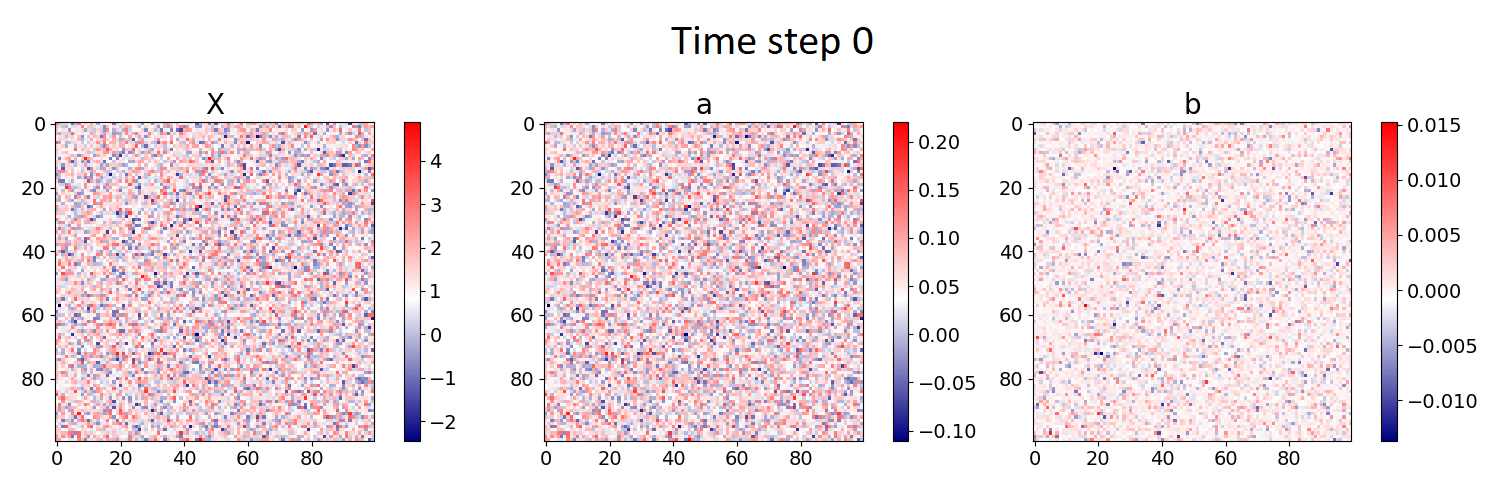
\includegraphics[width=\textwidth]{Flux_composite_00000}\\
	а)
	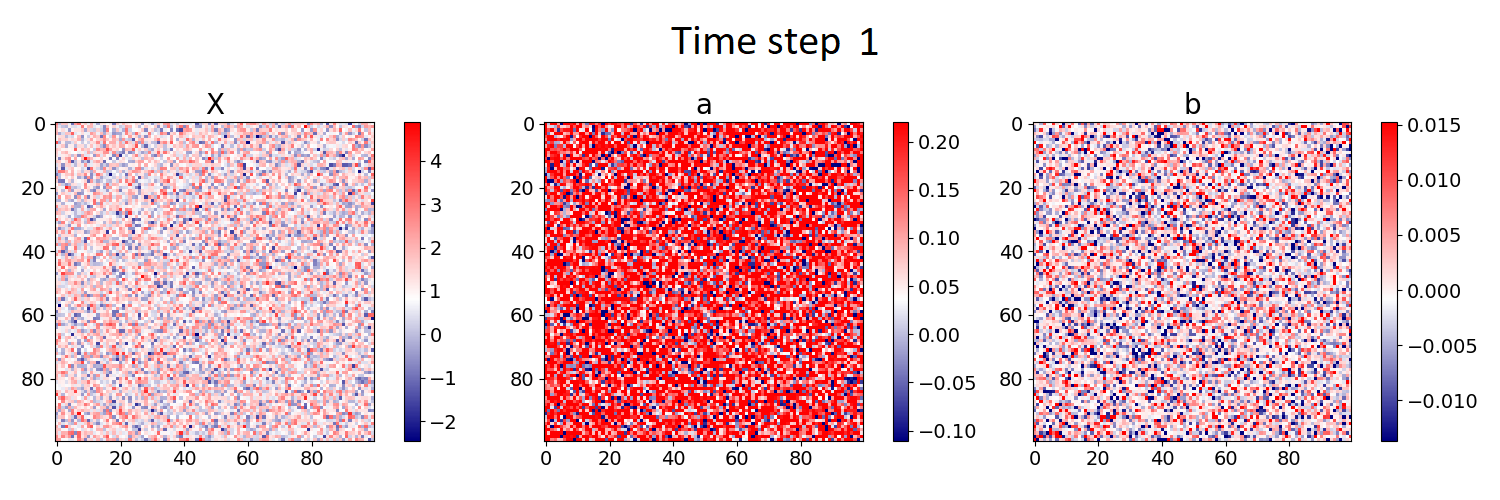
\includegraphics[width=\textwidth]{Flux_composite_00001}\\
	б)
	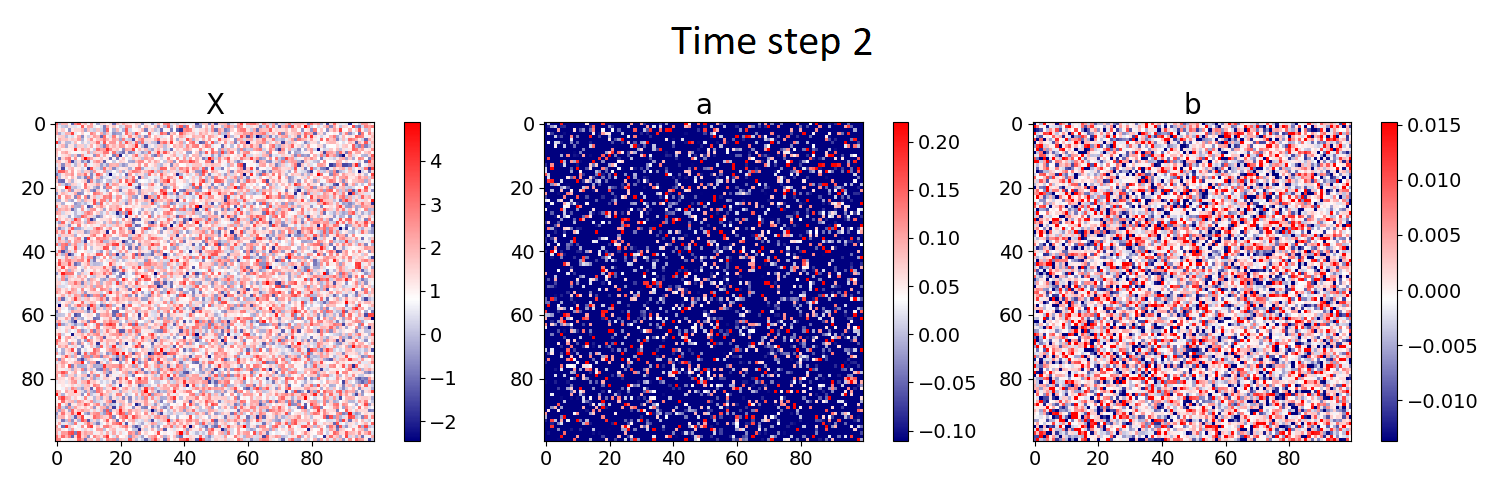
\includegraphics[width=\textwidth]{Flux_composite_00002}\\
	в)
	\caption{Моделируемый процесс $X$ и соответствующие коэффициенты $a$ и $b$ в моменты времени (a) $t=0$, (б) $t=1$, (в) $t=2$}
	\label{flux_simulation}
\end{figure}

На рисунке \ref{flux_simulation} показаны сгенерированные триплеты значений процесса и соответствующие коэффициенты $a(t,X)$ и $b(t,X)$ на первых трех последовательных этапах моделирования матриц размером $100 \times 100$. Оба метода, описанные в разделе 2, применяются к построенному процессу, и полученные в результате оценки коэффициентов сравниваются с определенными функциями $a(t,X)$ и $b(t,X)$.

\begin{figure}[!h]
	\centering
	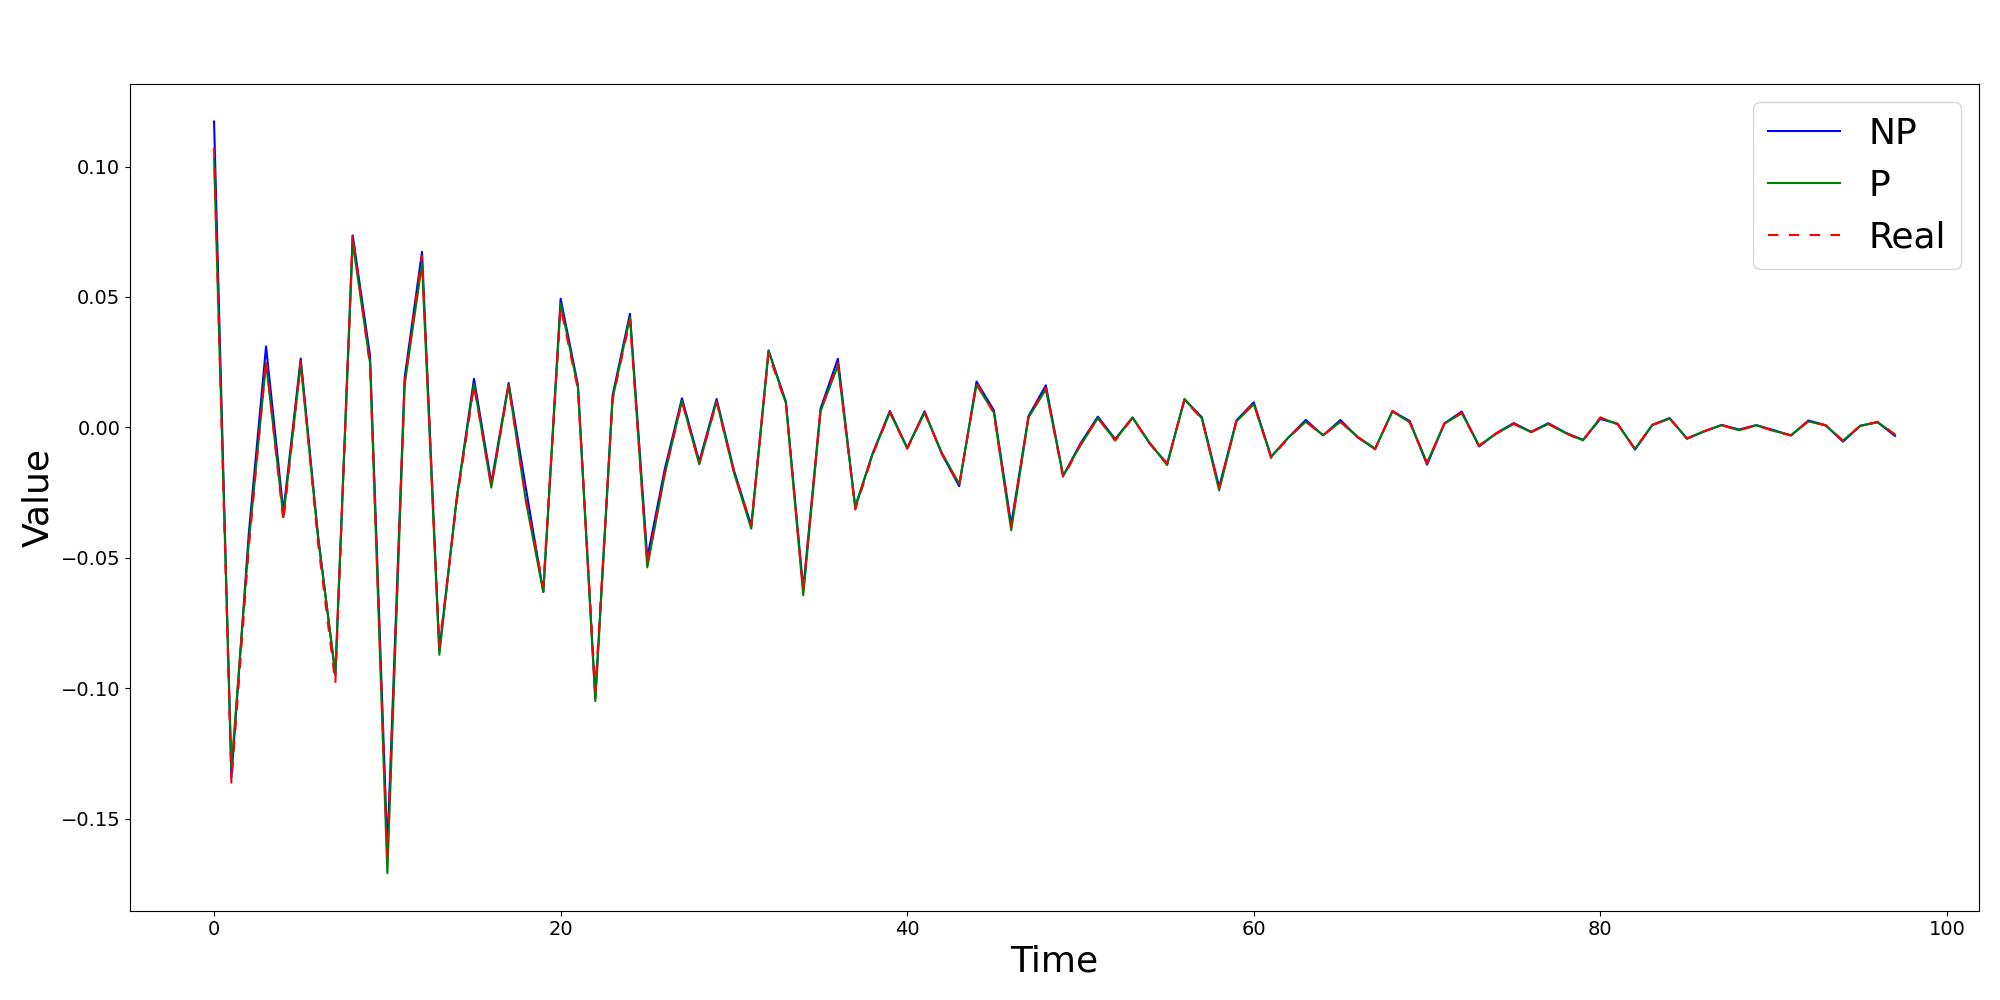
\includegraphics[width=\textwidth]{A_difference_point_(0, 4)-A}\\
	а)
	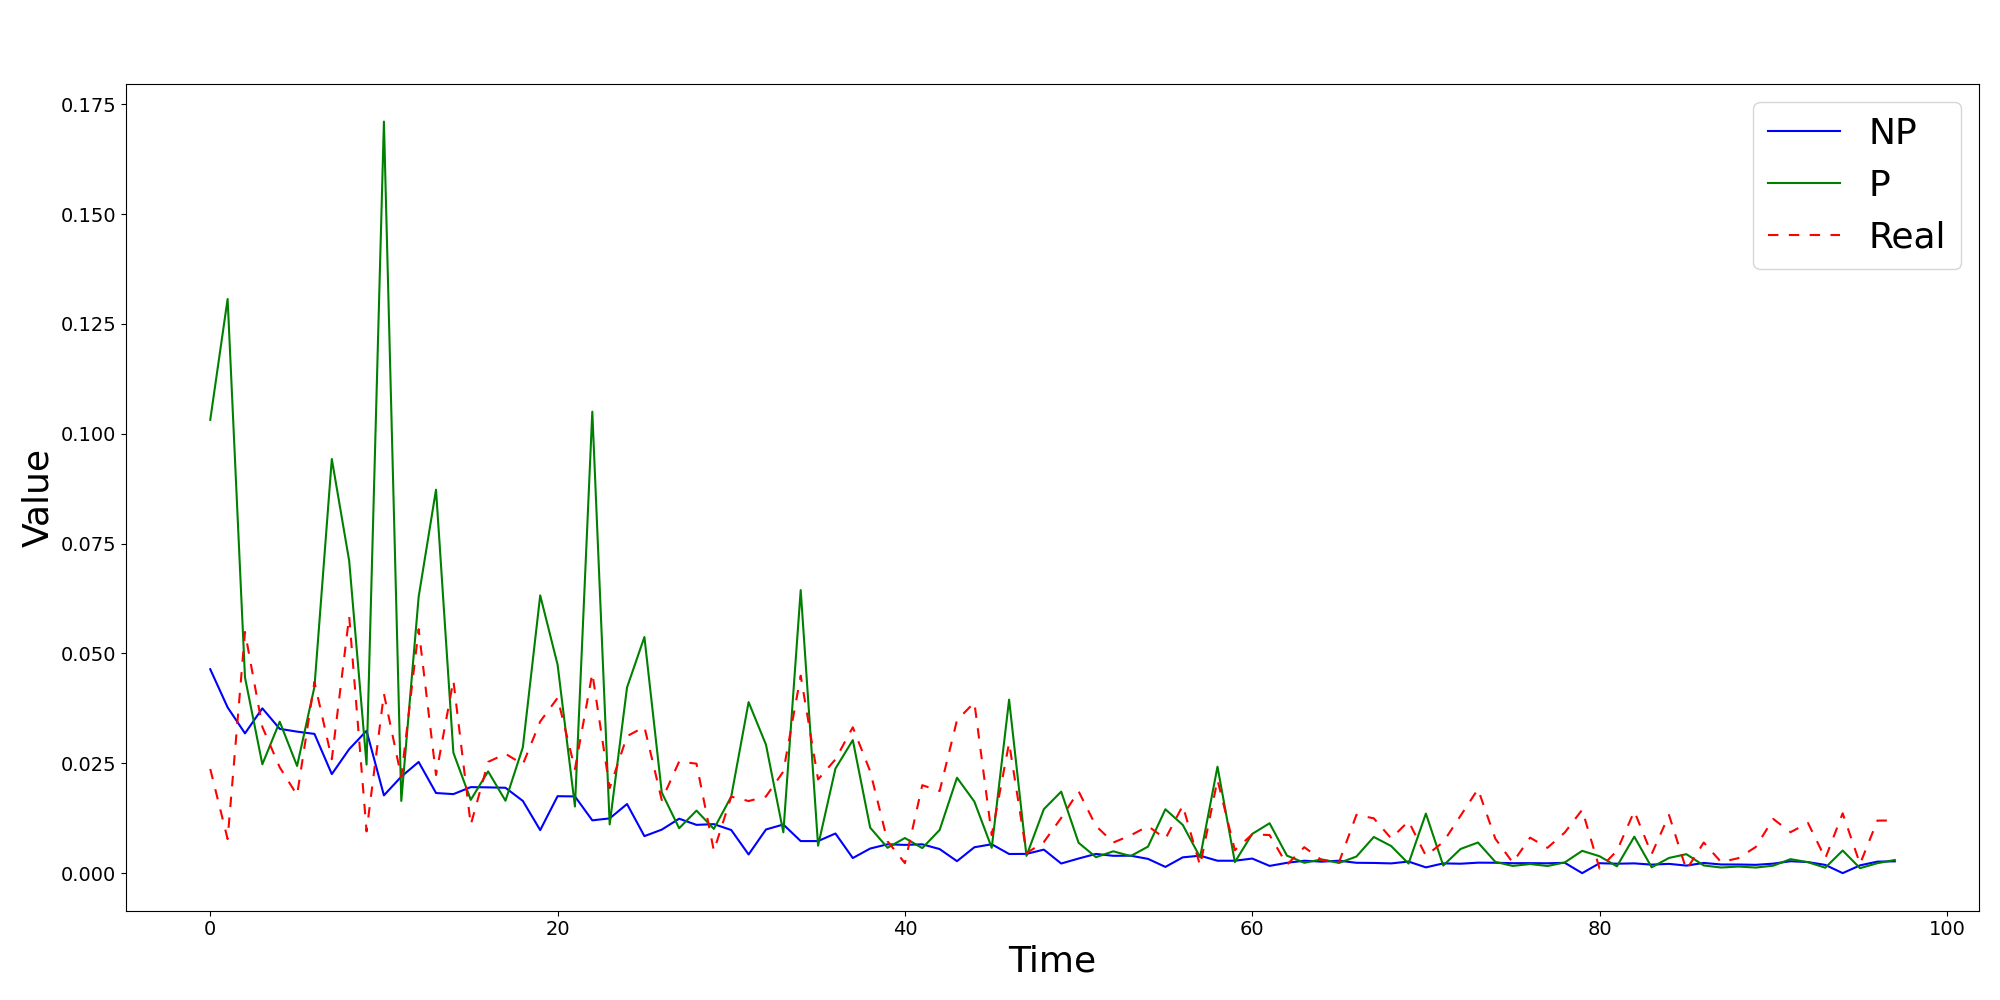
\includegraphics[width=\textwidth]{B_difference_point_(0, 4)-B}\\
	б)
	\caption{Сравнение полученных оценок коэффициентов $a(t,X)$ (а) и $b(t,X)$ (б) непараметрическим (NP) и параметрическим (P) методами с реальными значениями в точке $(0,4)$}
	\label{difference_0_4}
\end{figure}

\begin{figure}[!h]
	\centering
	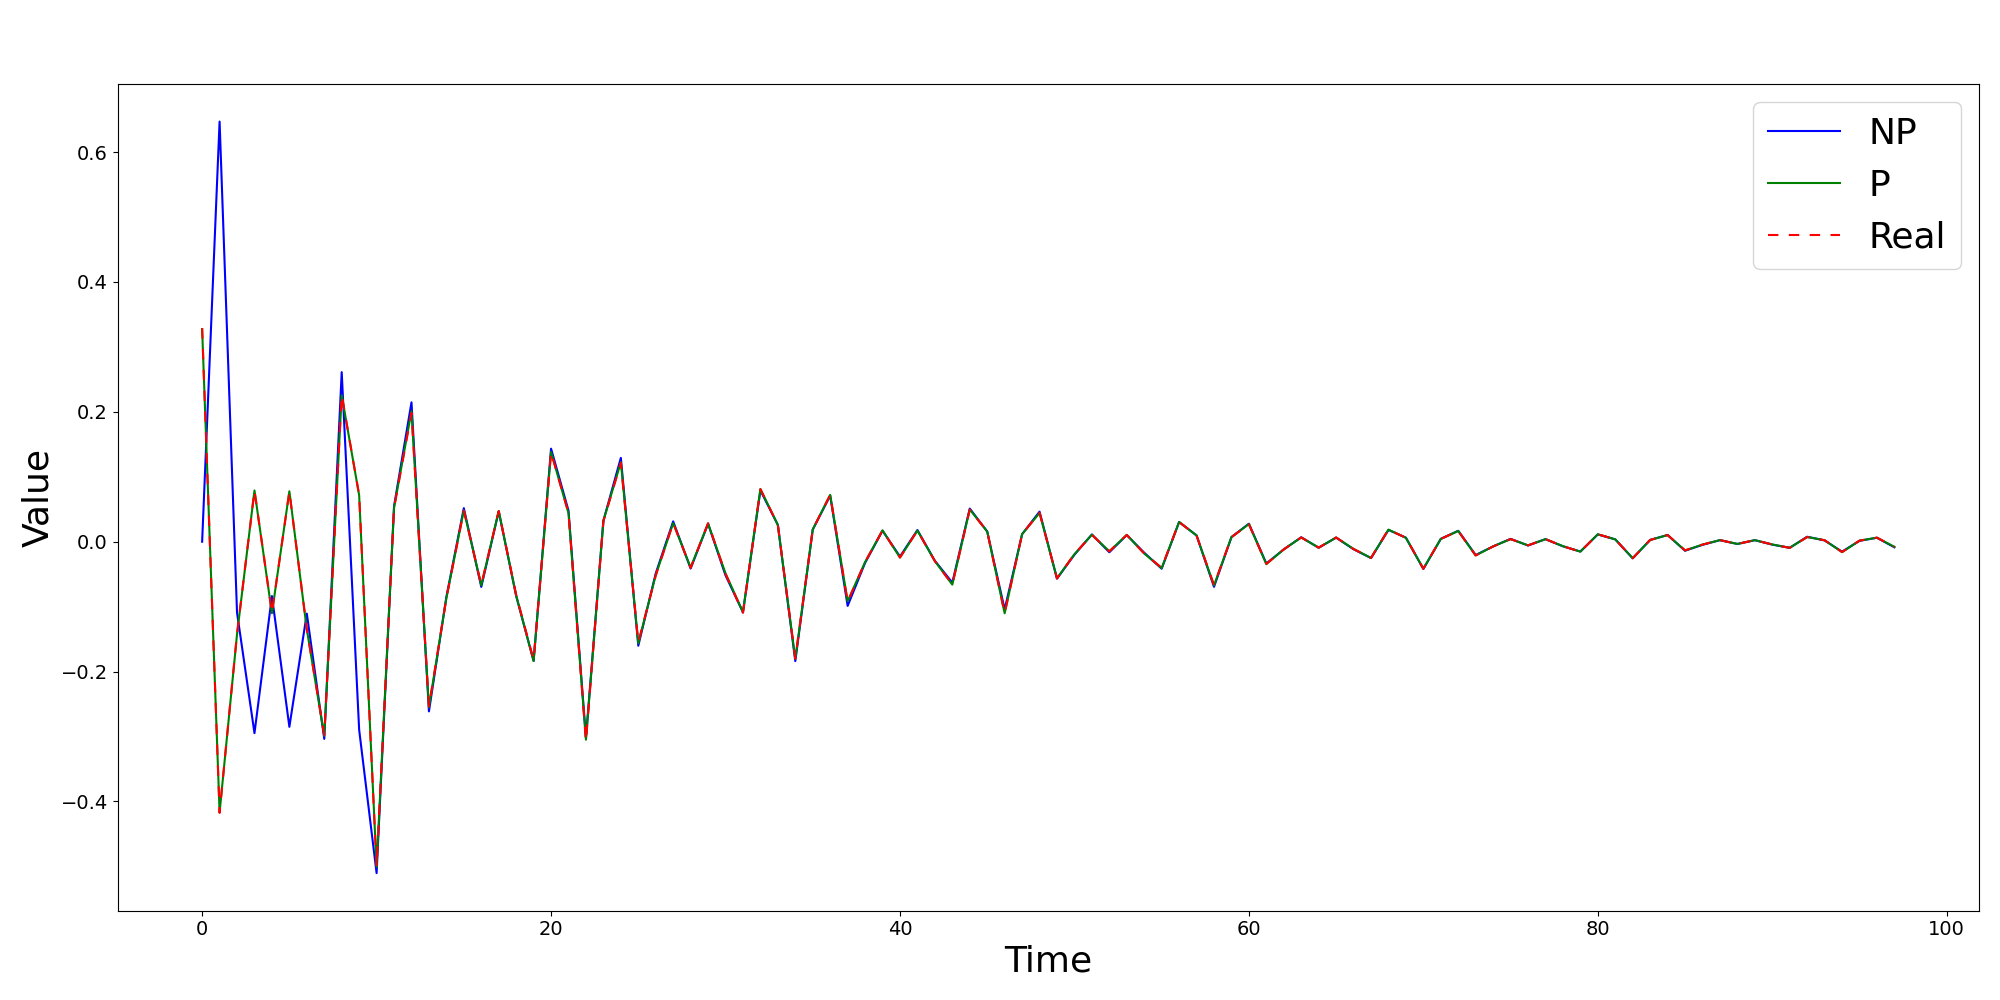
\includegraphics[width=\textwidth]{A_difference_point_(0, 11)-A}\\
	а)
	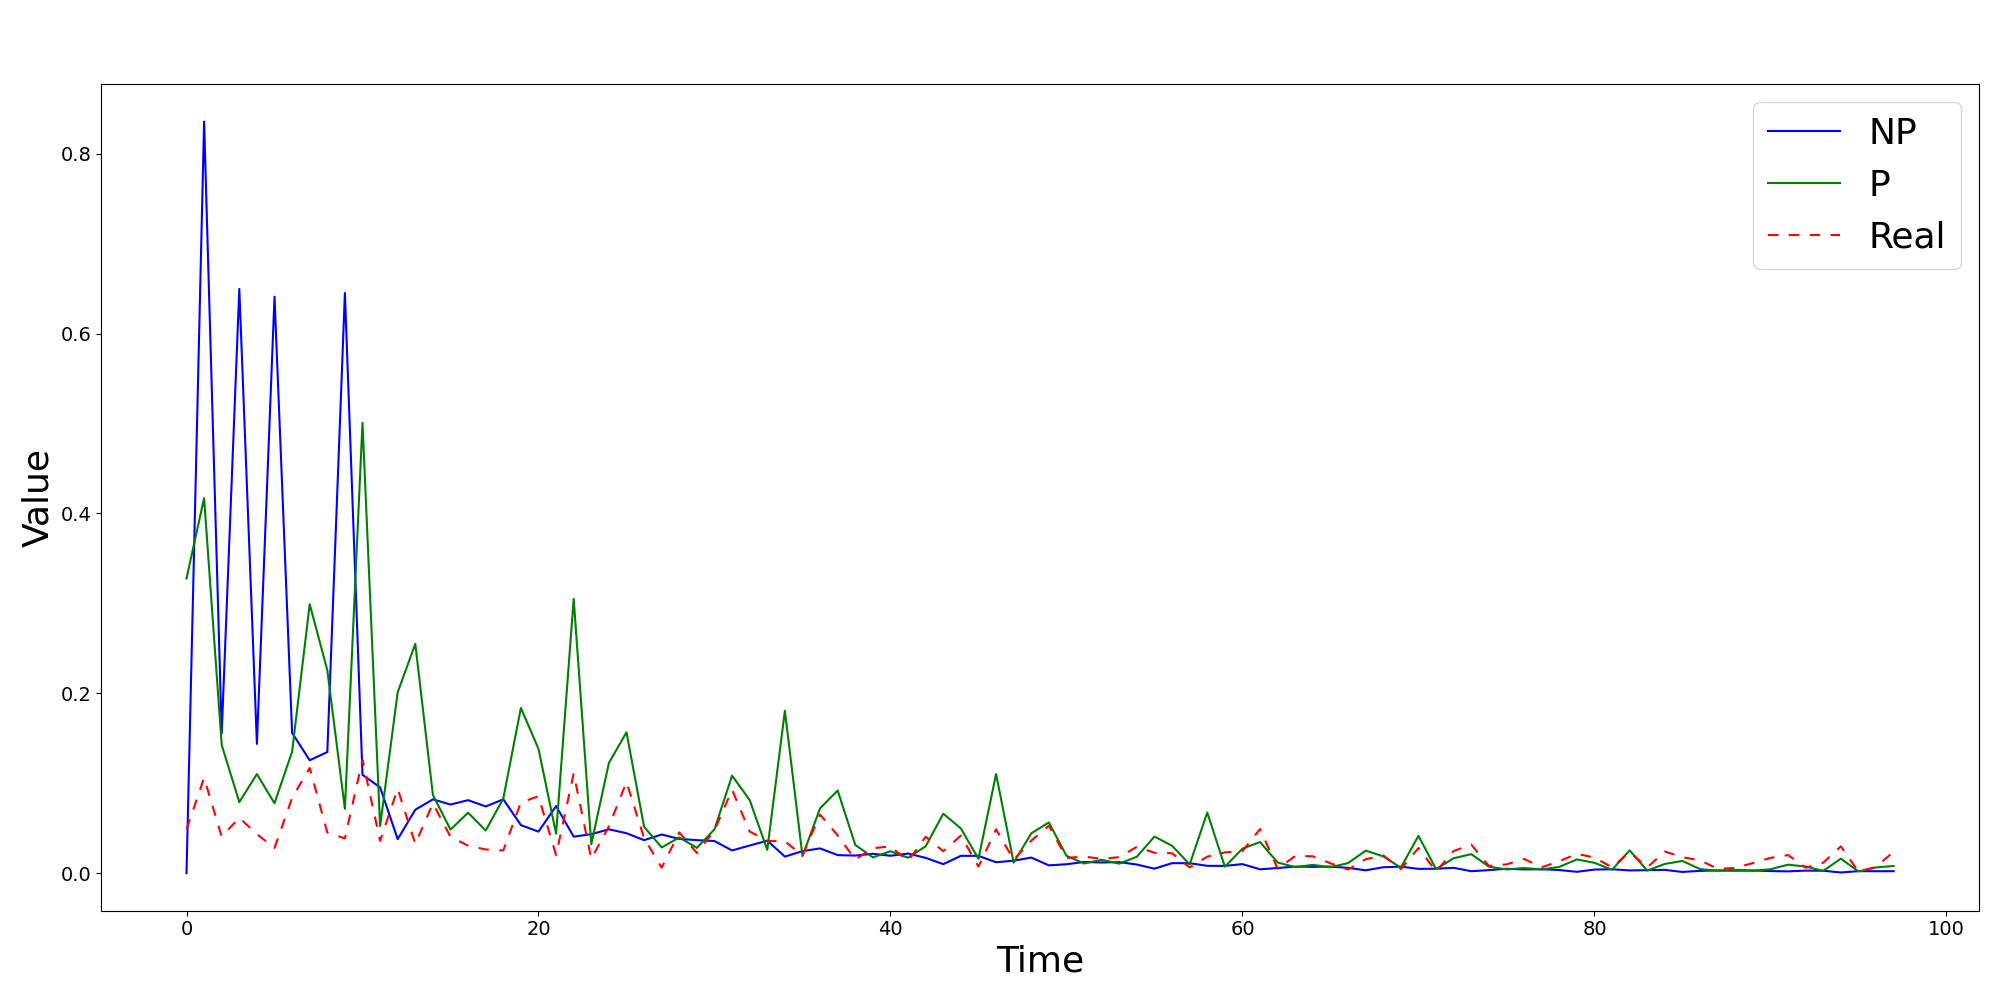
\includegraphics[width=\textwidth]{B_difference_point_(0, 11)-B}\\
	б)
	\caption{Сравнение полученных оценок коэффициентов $a(t,X)$ (а) и $b(t,X)$ (б) непараметрическим (NP) и параметрическим (P) методами с реальными значениями в точке $(0,11)$}
	\label{difference_0_11}
\end{figure}

\begin{figure}[!h]
	\centering
	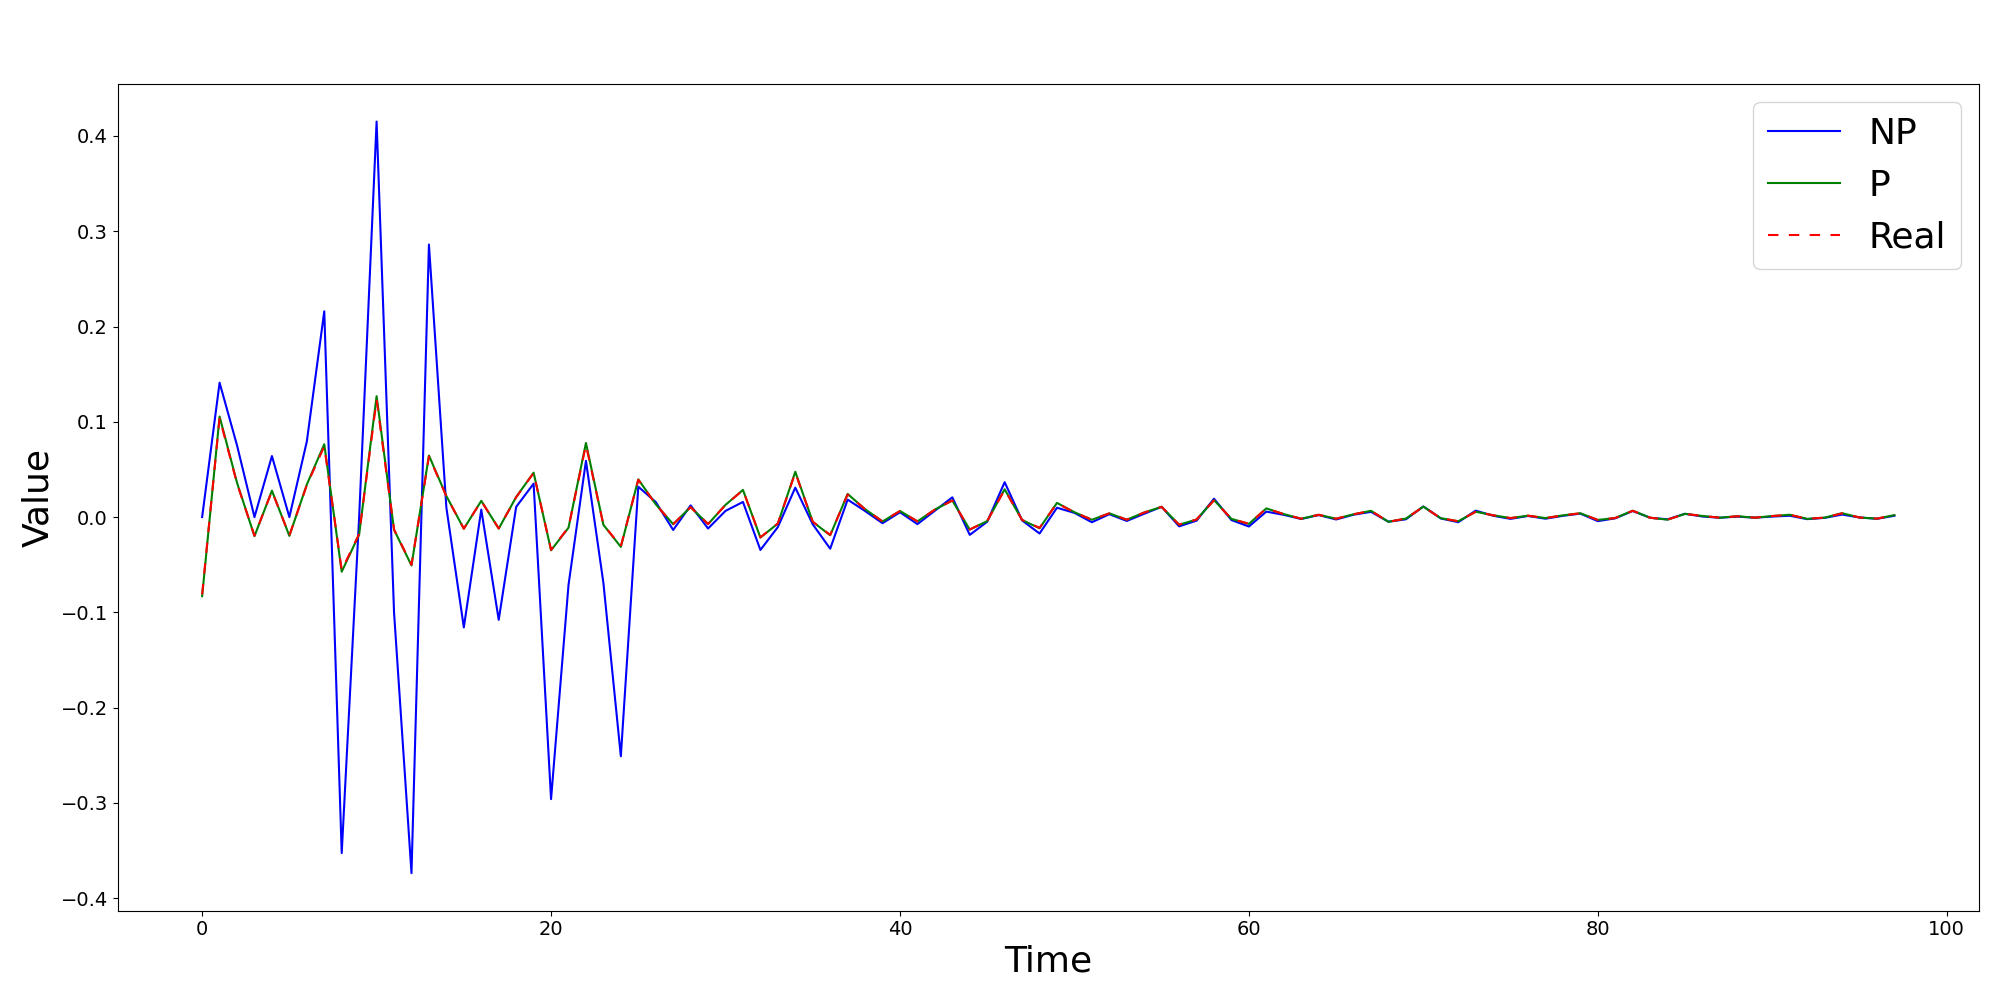
\includegraphics[width=\textwidth]{A_difference_point_(0, 27)-A}\\
	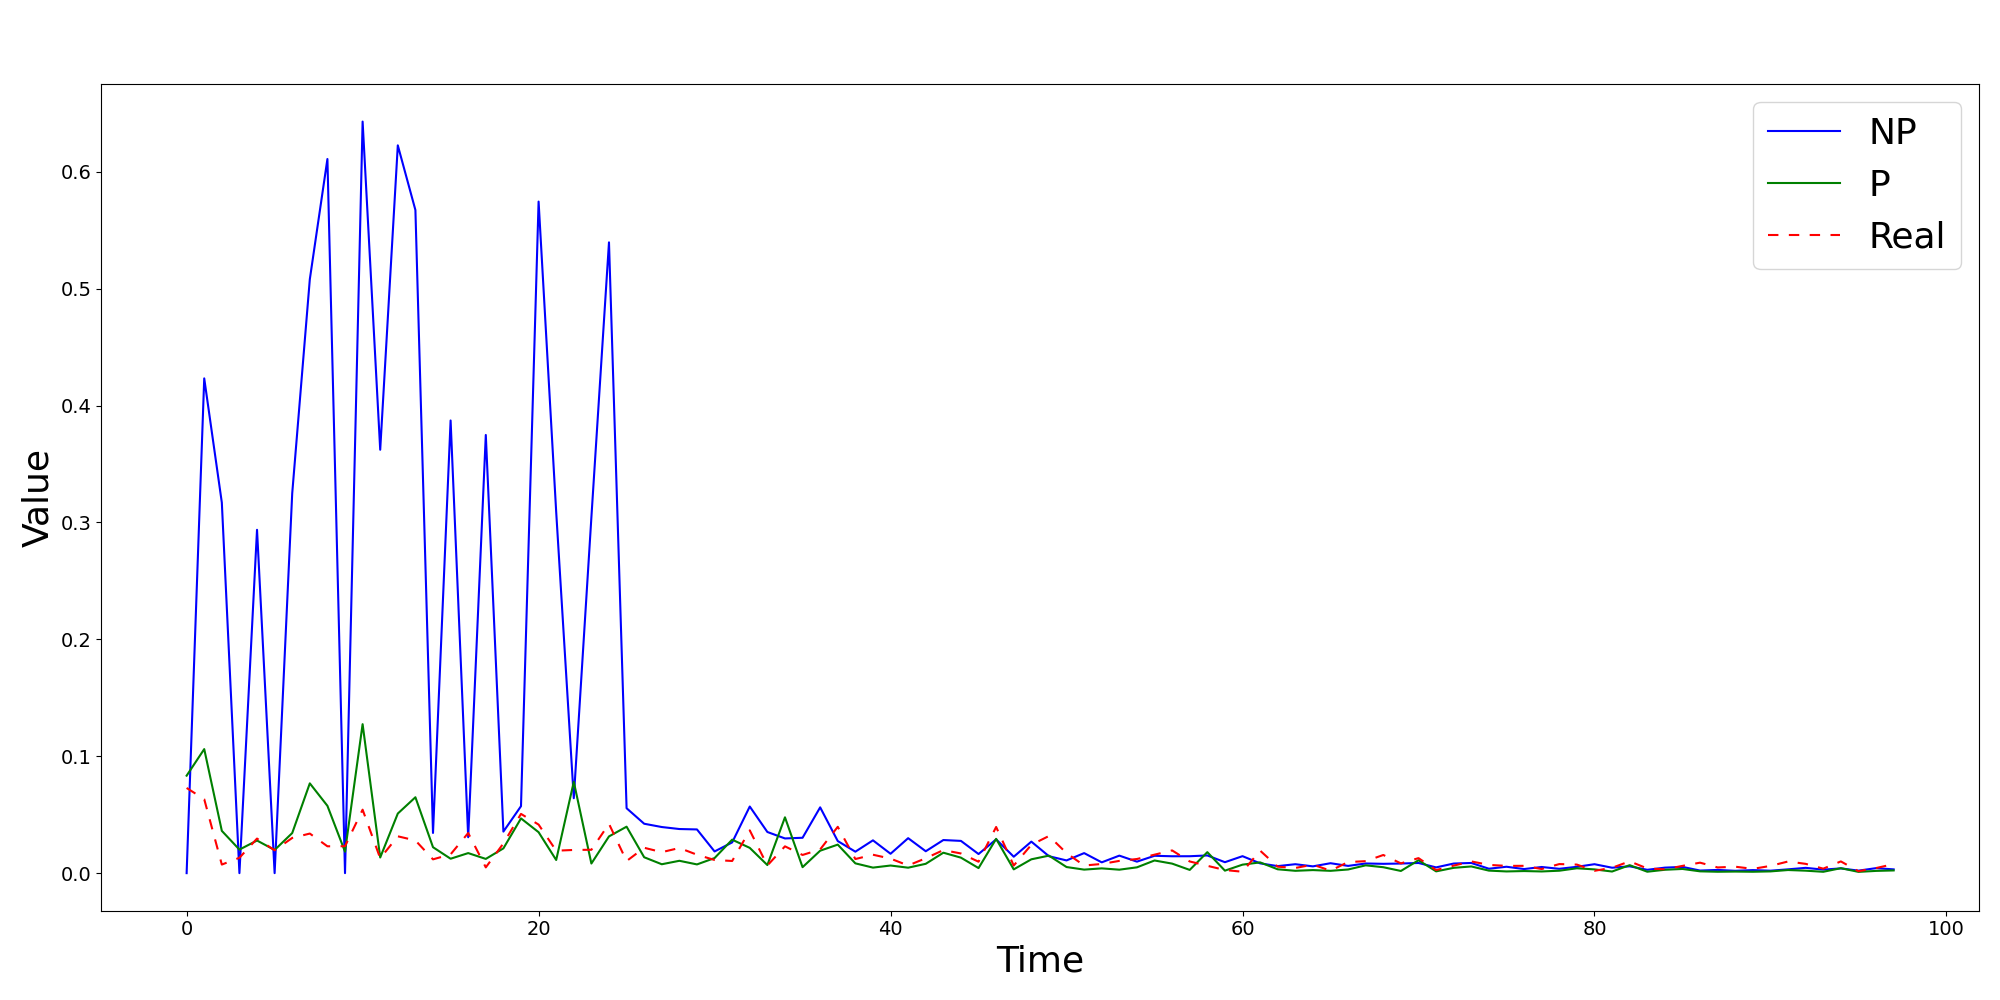
\includegraphics[width=\textwidth]{B_difference_point_(0, 27)-B}\\
	\caption{Сравнение полученных оценок коэффициентов $a(t,X)$ (а) и $b(t,X)$ (б) непараметрическим (NP) и параметрическим (P) методами с реальными значениями в точке $(0,27)$}
	\label{difference_0_27}
\end{figure}

На рисунках \ref{difference_0_4}--\ref{difference_0_27} показана эволюция целевых функций с шагом во времени и соответствующие оценки, полученные обоими методами в некоторых фиксированных точках матрицы (узлах сетки), демонстрирующие особенности обоих методов оценки. Ось времени показывает количество шагов генерации. Данные аналогичны показанным на рис. \ref{flux_simulation}, но за гораздо более длительный период времени (около $100$ итераций).
На рисунке \ref{difference_0_4} показан случай, в котором полупараметрический метод уступает непараметрическому с точки зрения RMSE, но гораздо лучше отражает поведение коэффициента диффузии. На рисунке \ref{difference_0_11} показана ситуация, в которой на первых этапах оба метода существенно отличаются от истинного значения коэффициента диффузии $b(t,X)$, но в последующие моменты времени полупараметрический метод начинает лучше описывать тенденцию, значительно превосходя кусочно-линейный вариант непараметрических оценок. Пример явного превосходства полупараметрического метода показан на рисунке \ref{difference_0_27}.

\begin{table}[h!]
	\centering
	\caption{Ошибки в оценках коэффициента $a(t,X)$ полупараметрическим и непараметрическим методами}
	\begin{tabular}{|c|c|c|}
		\hline
		Координаты точки & Полупараметрический метод & Непараметрический метод \\
		\hline
		$(0, 4)$ & $0.02$ & $0.01$ \\
		$(0, 11)$ & $1.28$ & $0.01$ \\
		$(0, 27)$ & $0.72$ & $0.01$ \\
		\hline
	\end{tabular}
	\label{table_errors_estimation_a}
\end{table}

\begin{table}[h!]
	\centering
	\caption{Ошибки в оценках коэффициента $b(t,X)$ полупараметрическим и непараметрическим методами}
	\begin{tabular}{|c|c|c|}
		\hline
		Координаты точки & Полупараметрический метод & Непараметрический метод \\
		\hline
		$(0, 4)$ & $0.14$ & $0.24$ \\
		$(0, 11)$ & $1.31$ & $0.75$ \\
		$(0, 27)$ & $1.75$ & $0.15$ \\
		\hline
	\end{tabular}
	\label{table_errors_estimation_b}
\end{table}

В таблицах \ref{table_errors_estimation_a} и \ref{table_errors_estimation_b} представлены результаты оценки коэффициентов с помощью обоих методов.

Стоит отметить, что оценки коэффициента дрейфа $a(t,X)$, полученные обоими методами во всех рассмотренных точках смоделированной карты, намного ближе к реальным значениям целевых функций, чем соответствующие оценки коэффициента диффузии $b(t,X)$ к их объективным значениям.

\subsection{Данные реанализа}
Теперь оба метода применяются к данным пространственно-временного повторного анализа тепловых потоков между океаном и атмосферой в Северной Атлантике за период $1979-2022$ годов. Для проверки и сравнения результатов методов на реальных данных используются данные повторного анализа из базы данных ERA5 для явных и скрытых тепловых потоков, описанные в разделе \ref{Data}.

\begin{figure}[!h]
	\centering
	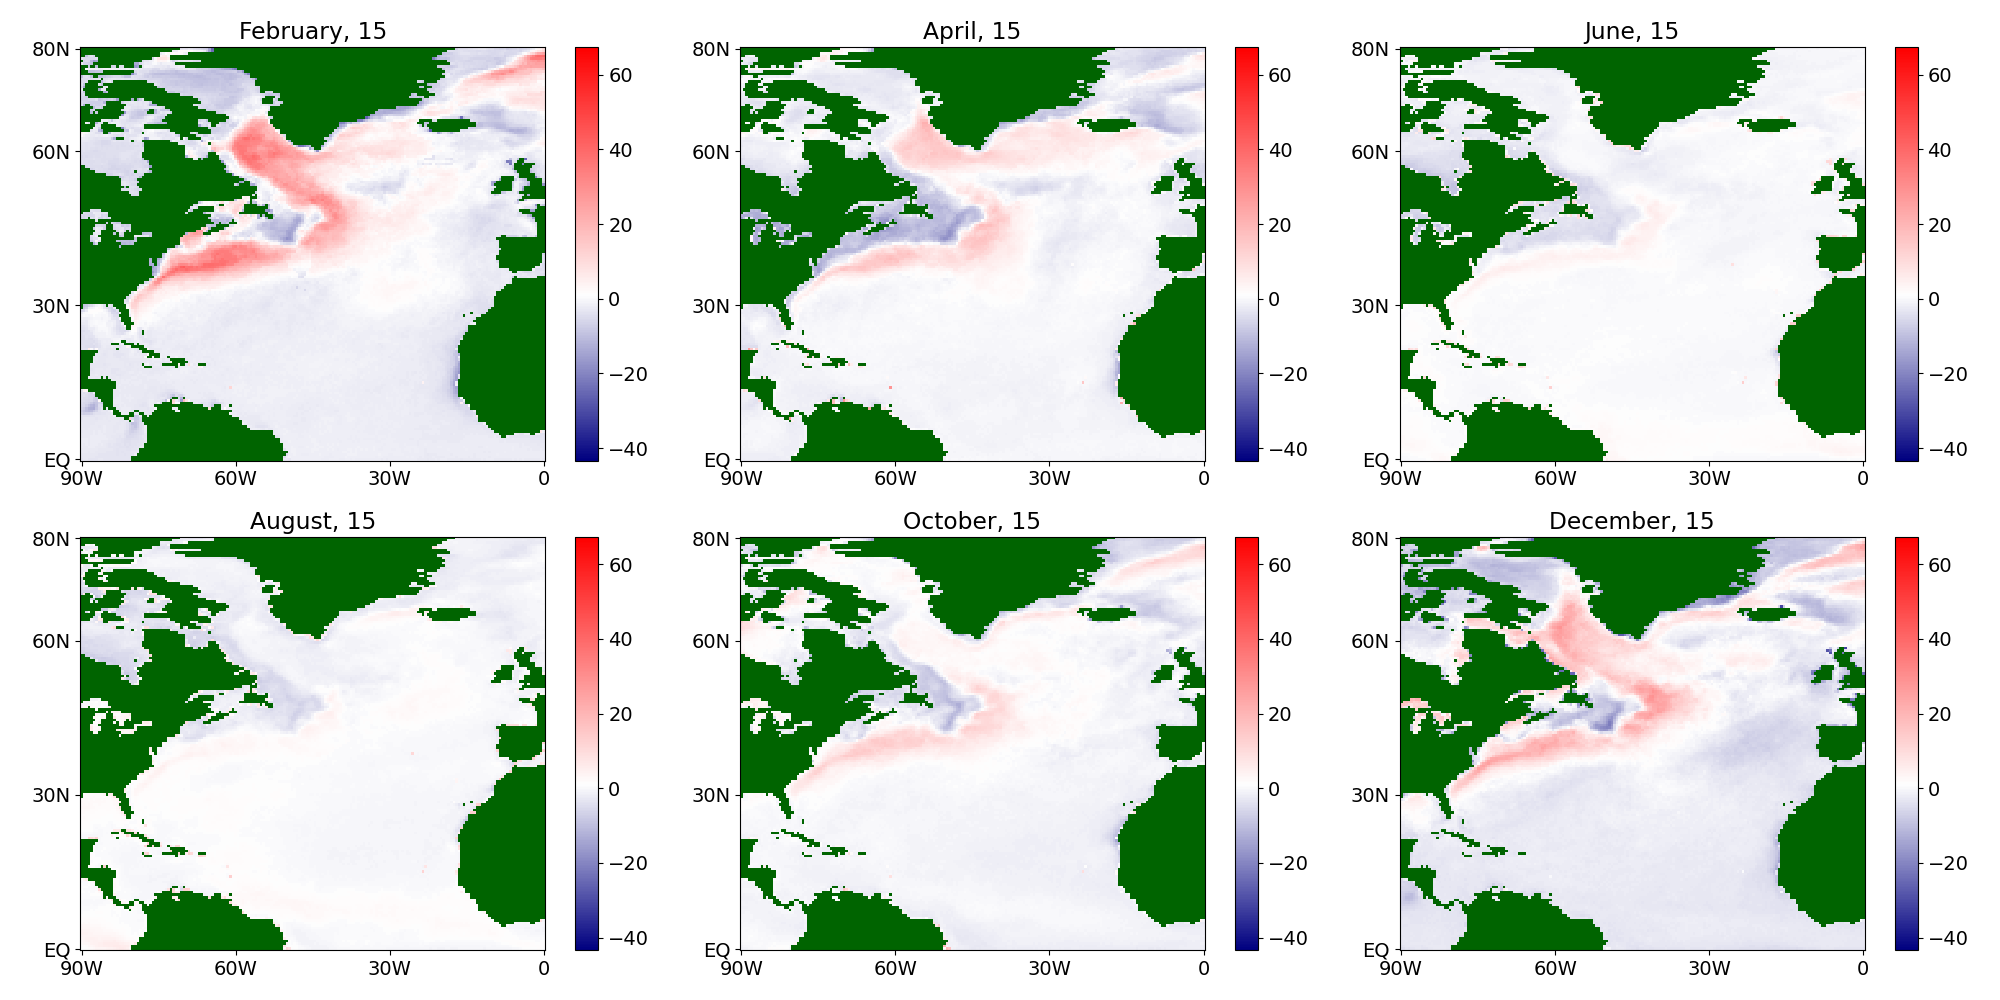
\includegraphics[width=\textwidth]{sensible_a_compare_semiparametric}\\
	а)
	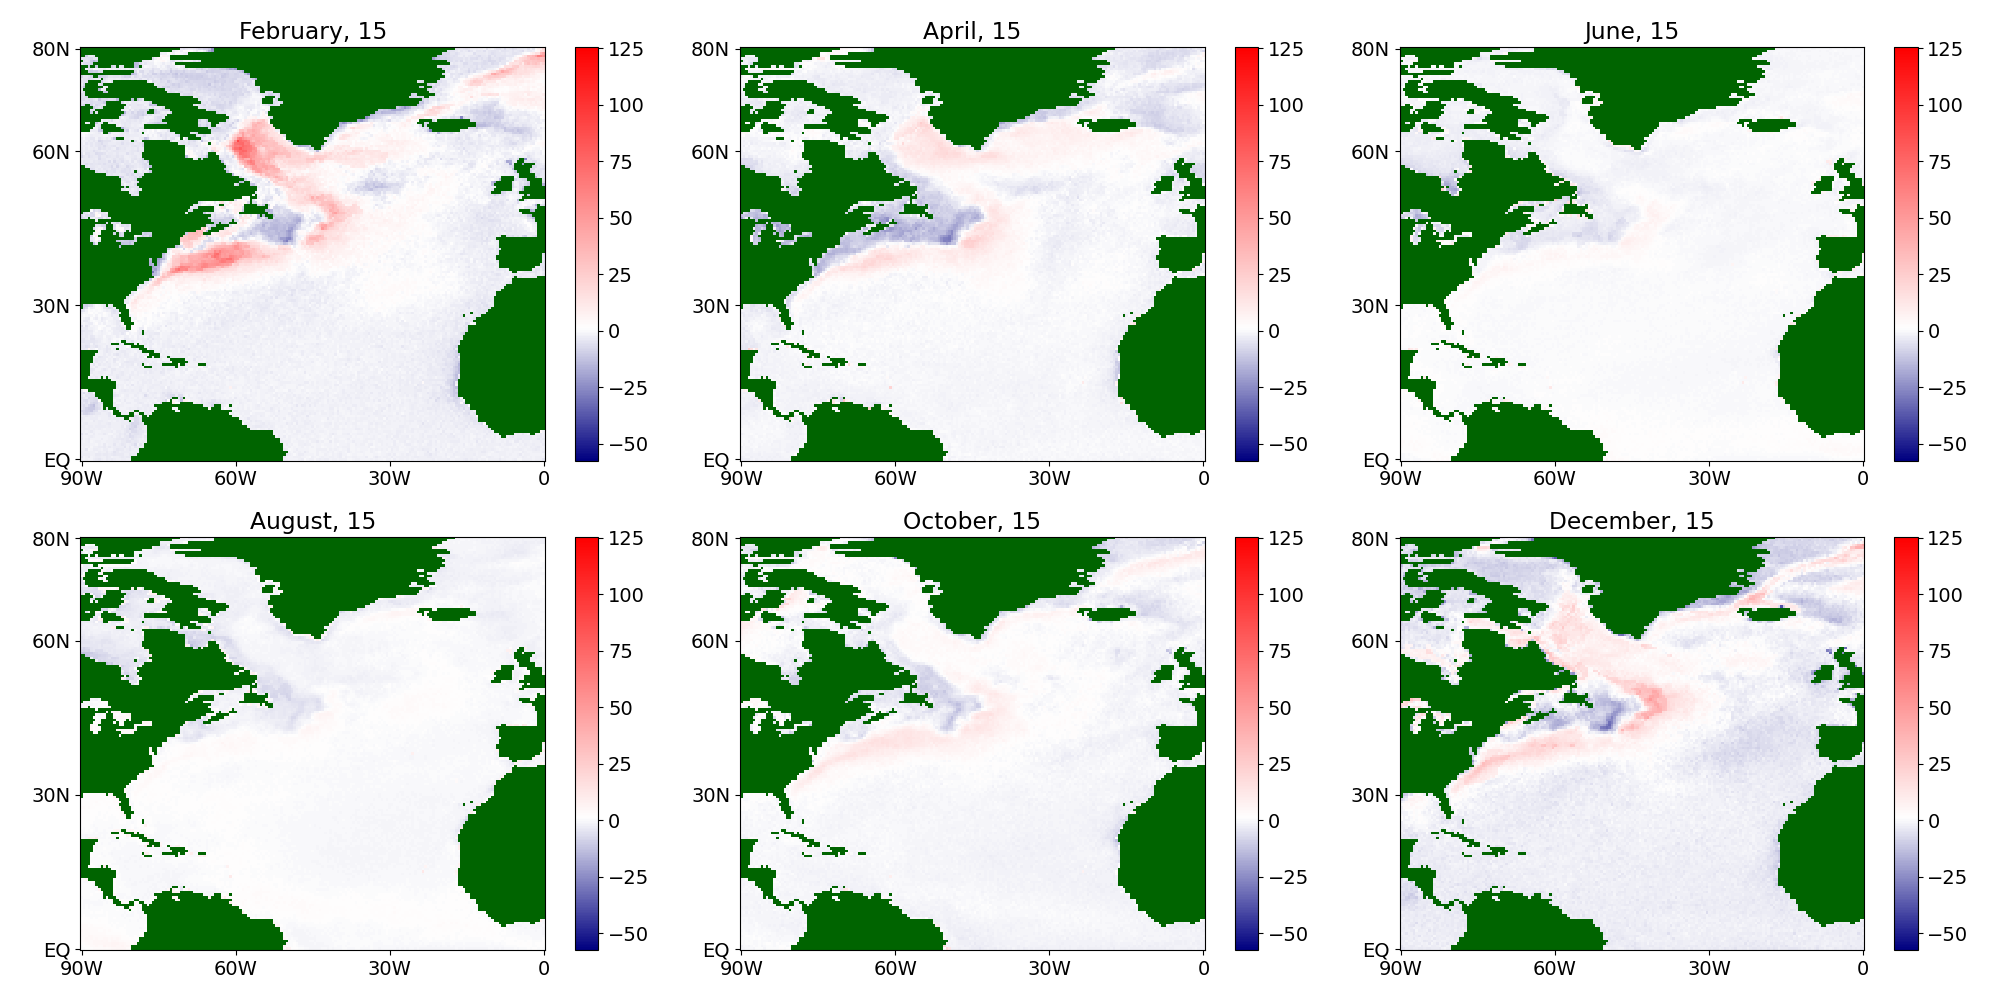
\includegraphics[width=\textwidth]{sensible_a_compare_nonparametric}\\
	б)
	\caption{Оценки коэффициента дрейфа для явного потока в течение среднего года за период $1979-2022$ гг., полученные с помощью (а) полупараметрического метода и (б) непараметрического метода.} 
	\label{fig_sensible_compare_a}
\end{figure}


\begin{figure}[!h]
	\centering
	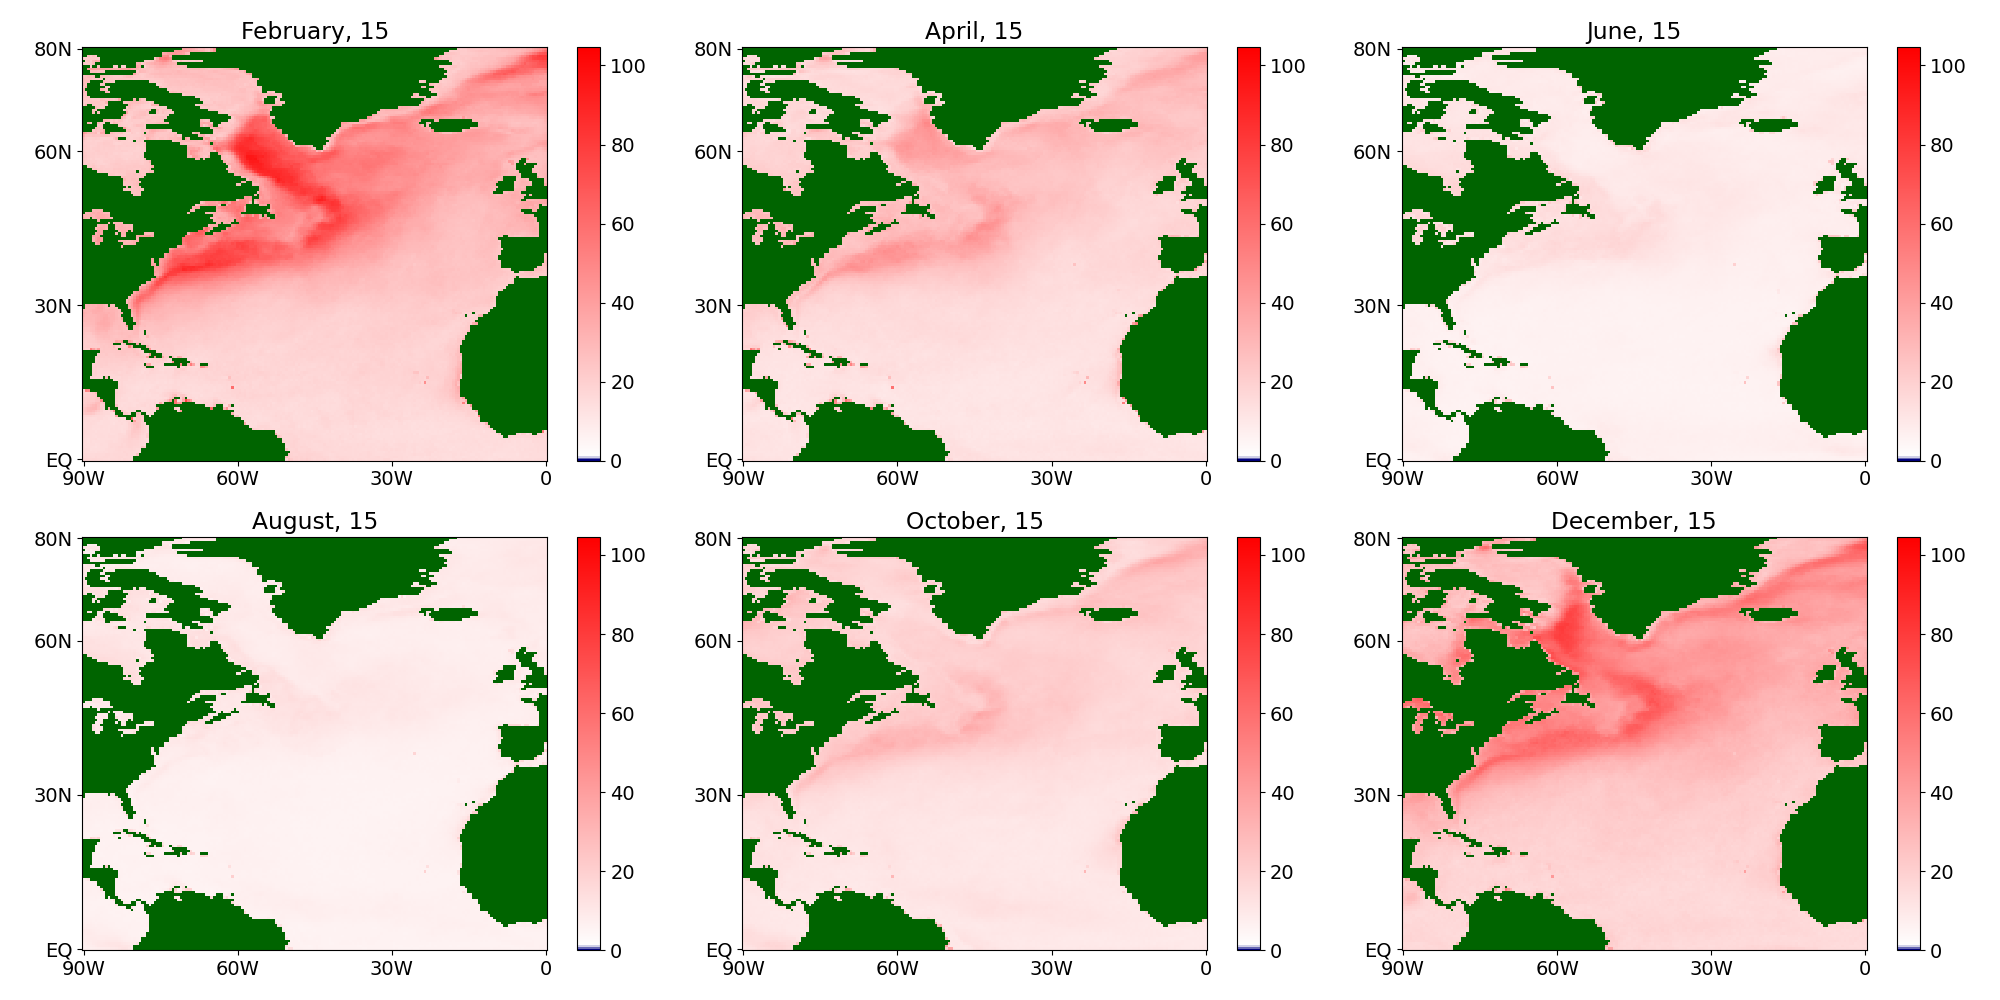
\includegraphics[width=\textwidth]{sensible_b_compare_semiparametric}\\
	а)
	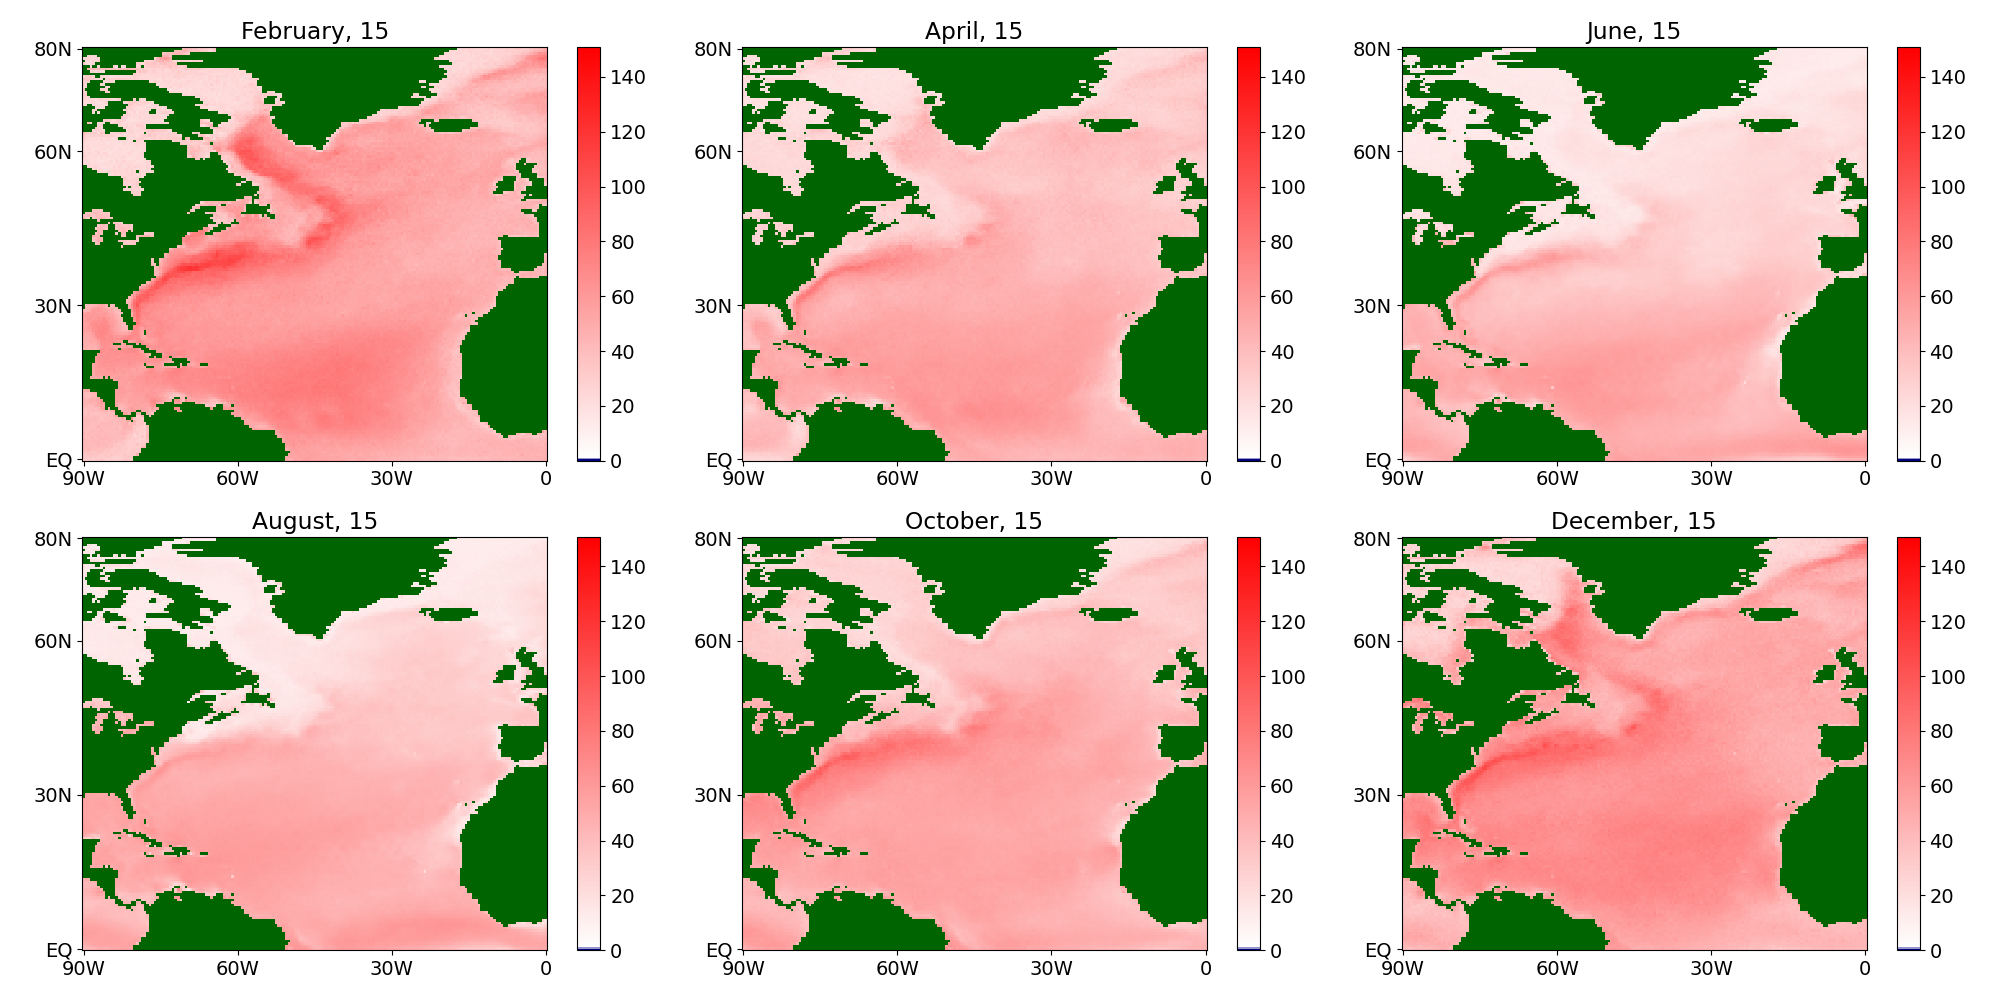
\includegraphics[width=\textwidth]{sensible_b_compare_nonparametric}\\
	б)
	\caption{Оценки коэффициента диффузии для явного потока в течение среднего года за период $1979-2022$ гг., полученные с помощью (а) полупараметрического метода и (б) непараметрического метода.} 
	\label{fig_sensible_compare_b}
\end{figure}

\begin{figure}[!h]
	\centering
	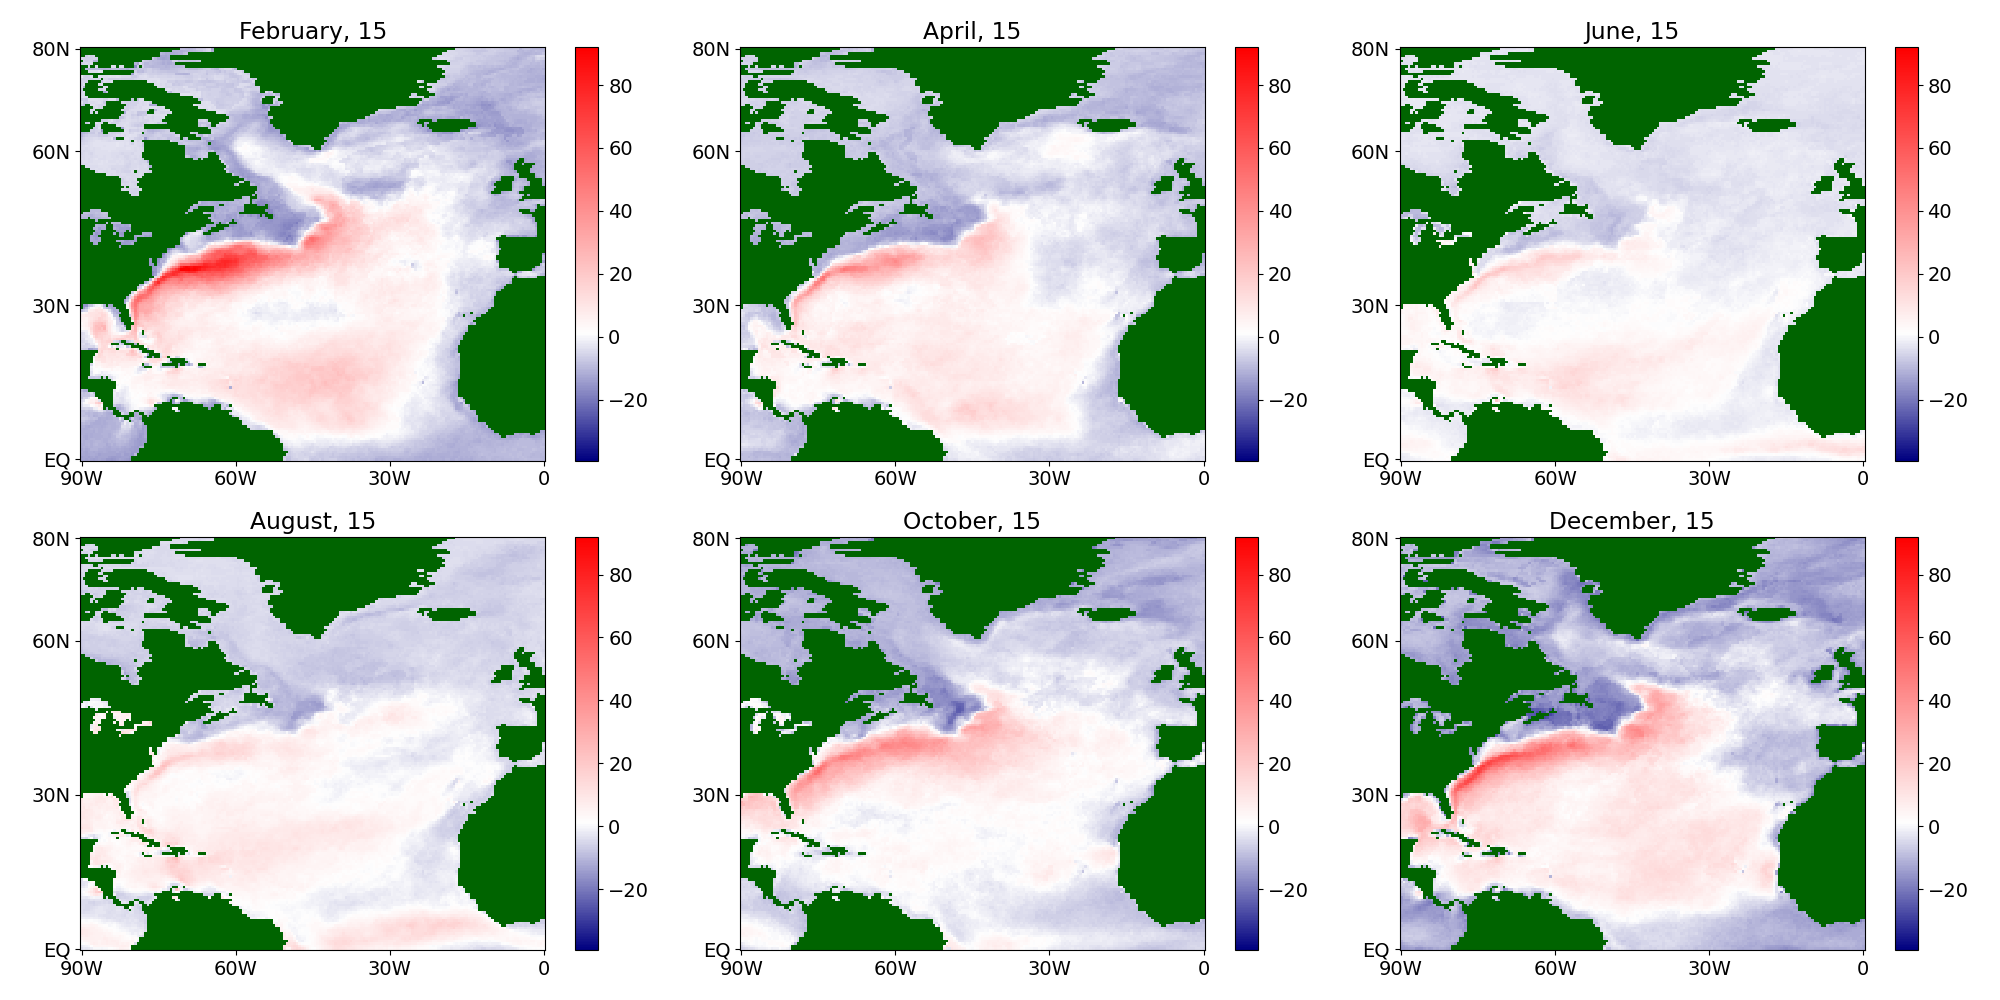
\includegraphics[width=\textwidth]{latent_a_compare_semiparametric}\\
	а)
	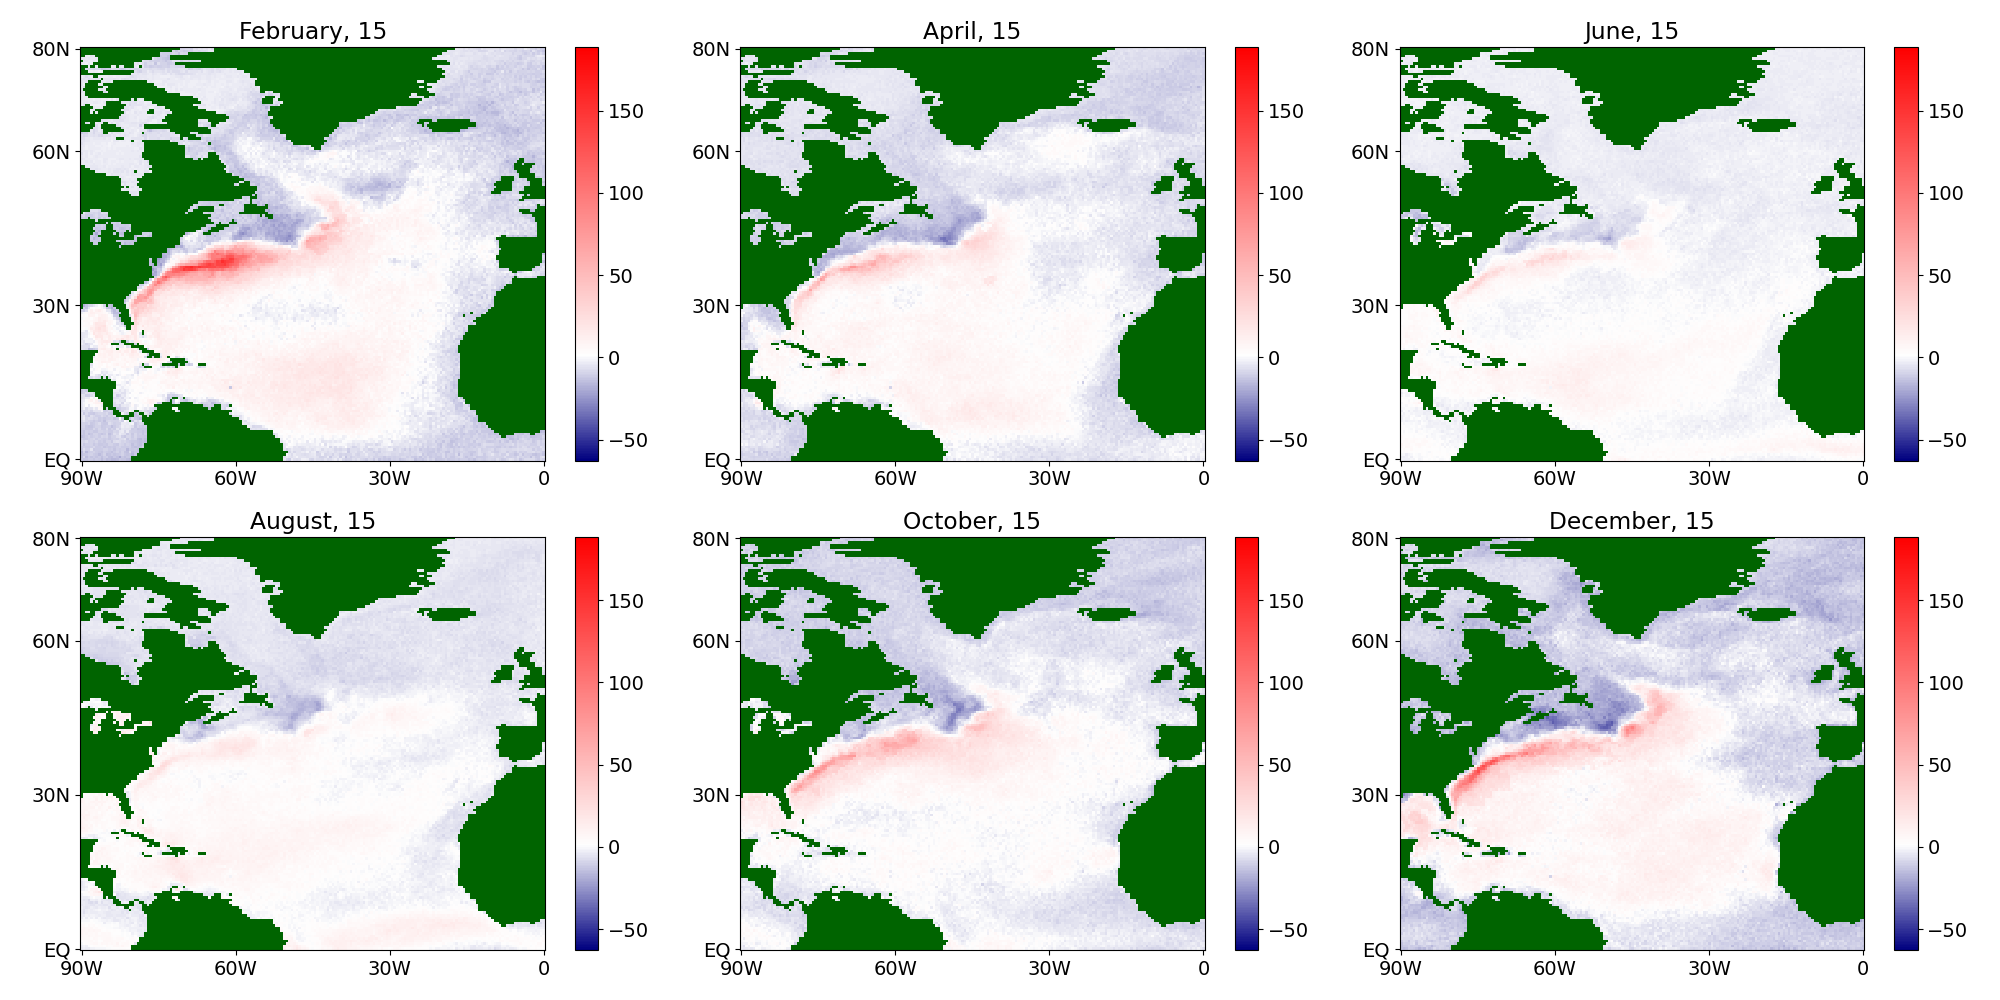
\includegraphics[width=\textwidth]{latent_a_compare_nonparametric}\\
	б)
	\caption{Оценки коэффициента дрейфа для скрытого потока в течение среднего года за период $1979-2022$ гг., полученные с помощью (а) полупараметрического метода и (б) непараметрического метода.} 
	\label{fig_latent_compare_a}
\end{figure}


\begin{figure}[!h]
	\centering
	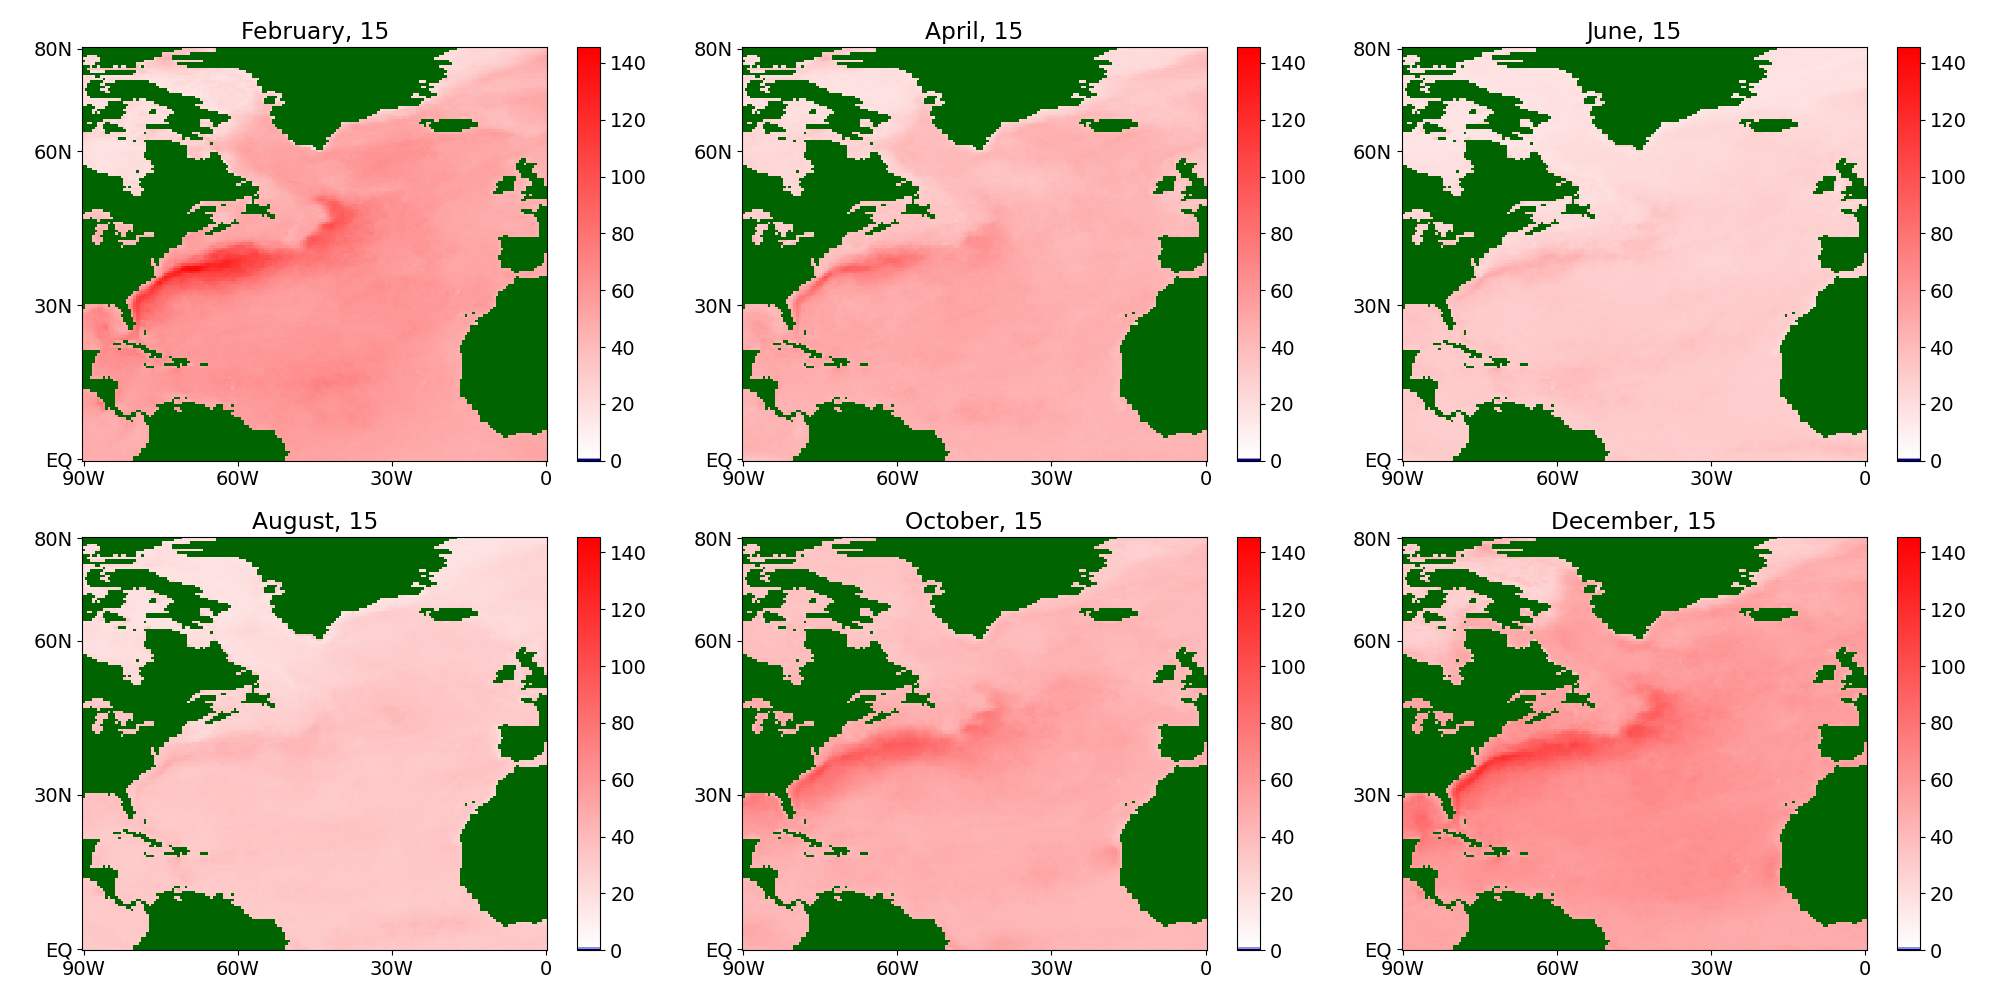
\includegraphics[width=\textwidth]{latent_b_compare_semiparametric}\\
	а)
	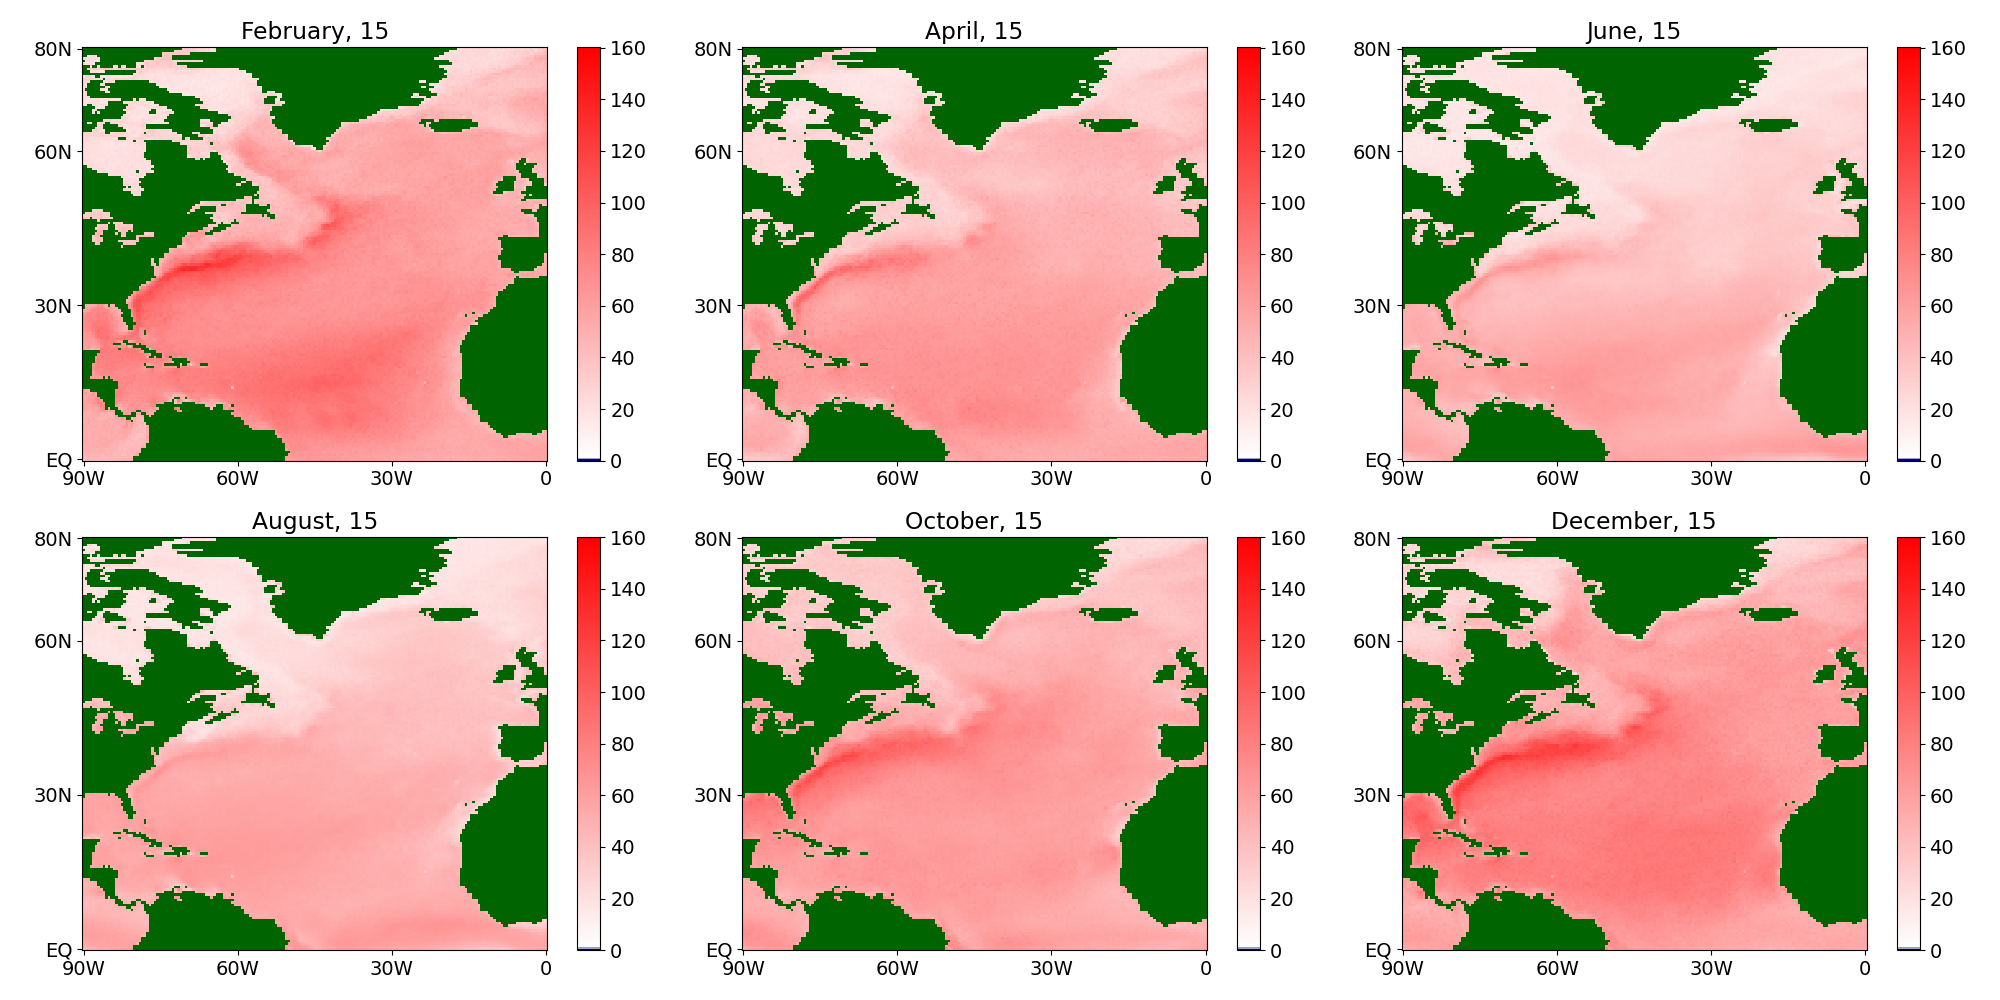
\includegraphics[width=\textwidth]{latent_b_compare_nonparametric}\\
	б)
	\caption{Оценки коэффициента диффузии для скрытого потока в течение среднего года за период $1979-2022$ гг., полученные с помощью (а) полупараметрического метода и (б) непараметрического метода.} 
	\label{fig_latent_compare_b}
\end{figure}

На рисунках \ref{fig_sensible_compare_a}-\ref{fig_latent_compare_b} показаны результаты обоих методов для явных и скрытых тепловых потоков в течение так называемого “среднего года”, которые построены следующим образом: в каждый из шести выбранных фиксированных дней в году в разное время года (а именно, 15 февраля, 15 апреля, 15 июня, 15 августа, 15 октября, и 15 декабря), полученные оценки усредняются по всем рассматриваемым годам. Это позволяет сгладить отдельные выбросы, возникающие как непосредственно в самих данных, так и из-за вычислительных ошибок при расчете точечных оценок. Результаты применения непараметрического метода к тем же данным и их анализ с геофизической точки зрения за этот период можно найти в работе~\cite{Gorshenin2023}.
Цветовая гамма на картах меняется с синего (при отрицательных значениях) на белый (при значениях, близких к нулю) и далее на красный (при положительных значениях). Яркость цвета в определенной точке соответствует расстоянию значения от нуля. Участки местности отмечены темно-зеленым цветом. Очевидно, что на картах, соответствующих оценкам коэффициента диффузии, синий цвет не отображается, поскольку значения неотрицательны (с физической точки зрения коэффициент диффузии эквивалентен дисперсии случайной величины).
На рисунке \ref{fig_sensible_compare_a} показан пример значений полученных оценок, полученных с помощью обоих методов, для коэффициента дрейфа для ощутимого потока в течение среднего года. Видно, что визуально они очень сильно совпадают, но оценки, полученные полупараметрическим методом, более плавно меняют цвет в соседних узлах карты (то есть имеют более близкие значения), а также имеют значения в областях пиков, которые в абсолютном выражении меньше, чем соответствующие полученные с помощью непараметрического метода. Тенденция изменения максимальных абсолютных значений, как и ожидалось, хорошо соответствует зонам сильных струйных течений в Северной Атлантике. Также наблюдается сезонный цикл: в зимние месяцы коэффициент дрейфа положительный, тогда как в летние месяцы он отрицательный.

Локализация, полученная с помощью непараметрического метода, является более грубой и точной, но менее детализированной, чем локализация, полученная с помощью полупараметрического метода. Аналогичные выводы справедливы и для коэффициента диффузии (см. рис. \ref{fig_sensible_compare_b}), хотя указанный эффект оказывается менее выраженным. Он характеризуется обширными зонами своего максимального значения и менее выраженным сезонным циклом, чем для соответствующего коэффициента дрейфа, хотя в летние месяцы максимум заметно меньше в обоих методах, как для явных, так и для скрытых потоков. На рисунках \ref{fig_latent_compare_a} и \ref{fig_latent_compare_b} представлены те же коэффициенты для скрытых потоков.

\begin{figure}[!h]
	\centering
	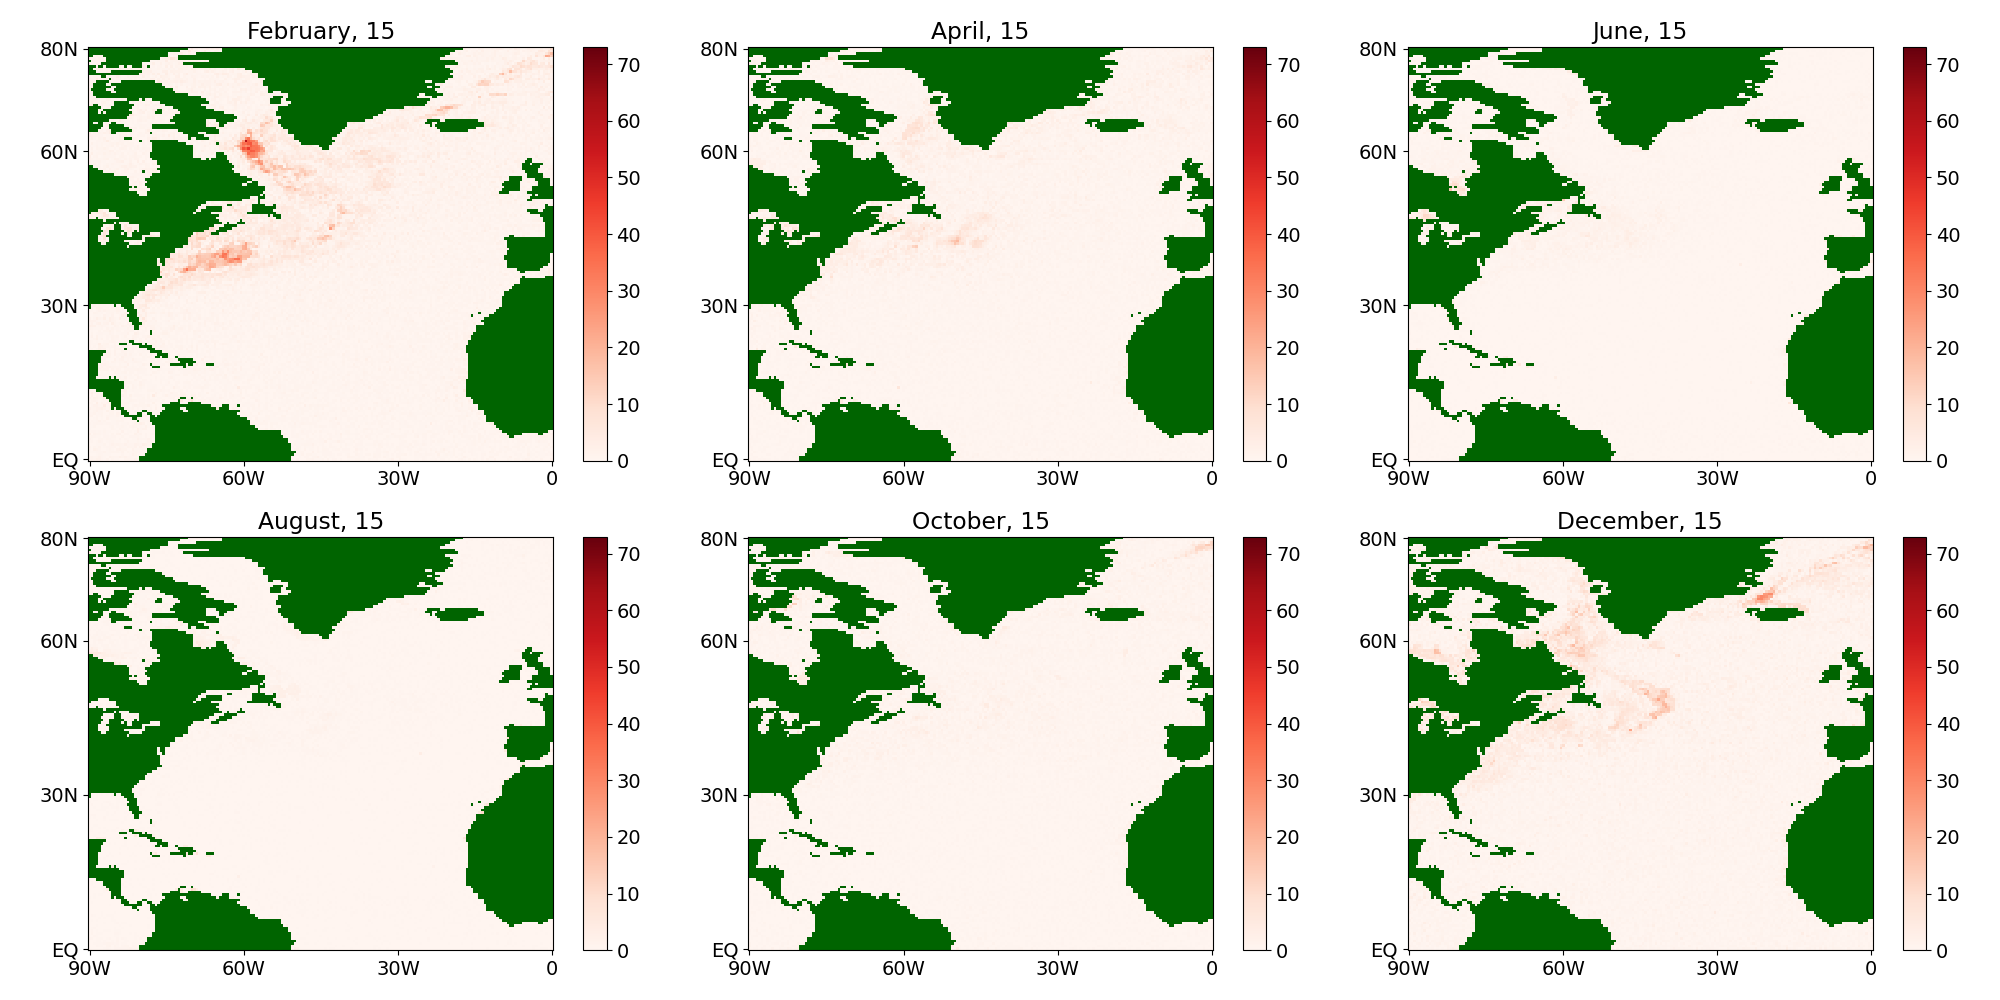
\includegraphics[width=\textwidth]{difference_a_compare_sensible}
	\caption{Абсолютная разность оценок коэффициента дрейфа для явного потока в течение среднего года за период $1979-2022$ гг.} 
	\label{fig_sensible_difference_a}
\end{figure}


\begin{figure}[!h]
	\centering
	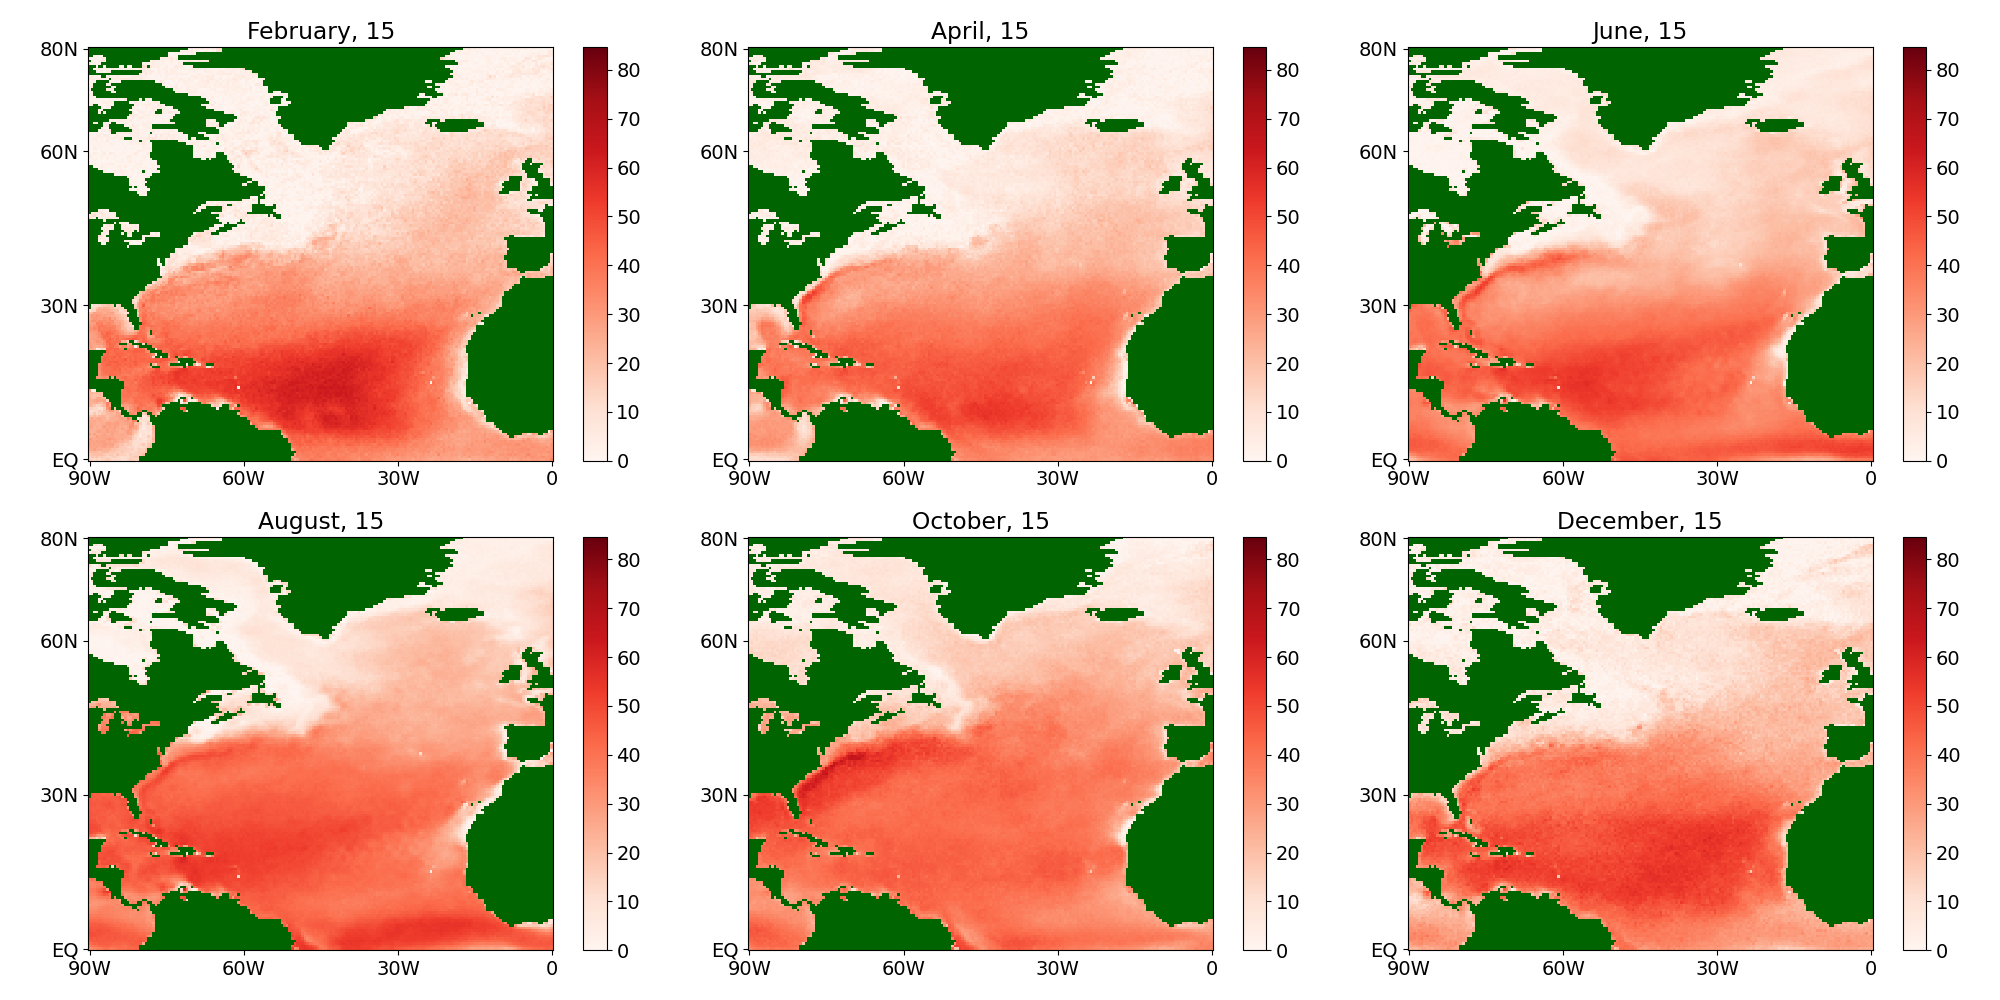
\includegraphics[width=\textwidth]{difference_b_compare_sensible}
	\caption{Абсолютная разность оценок коэффициента диффузии для явного потока в течение среднего года за период $1979-2022$ гг.} 
	\label{fig_sensible_difference_b}
\end{figure}

\begin{figure}[!h]
	\centering
	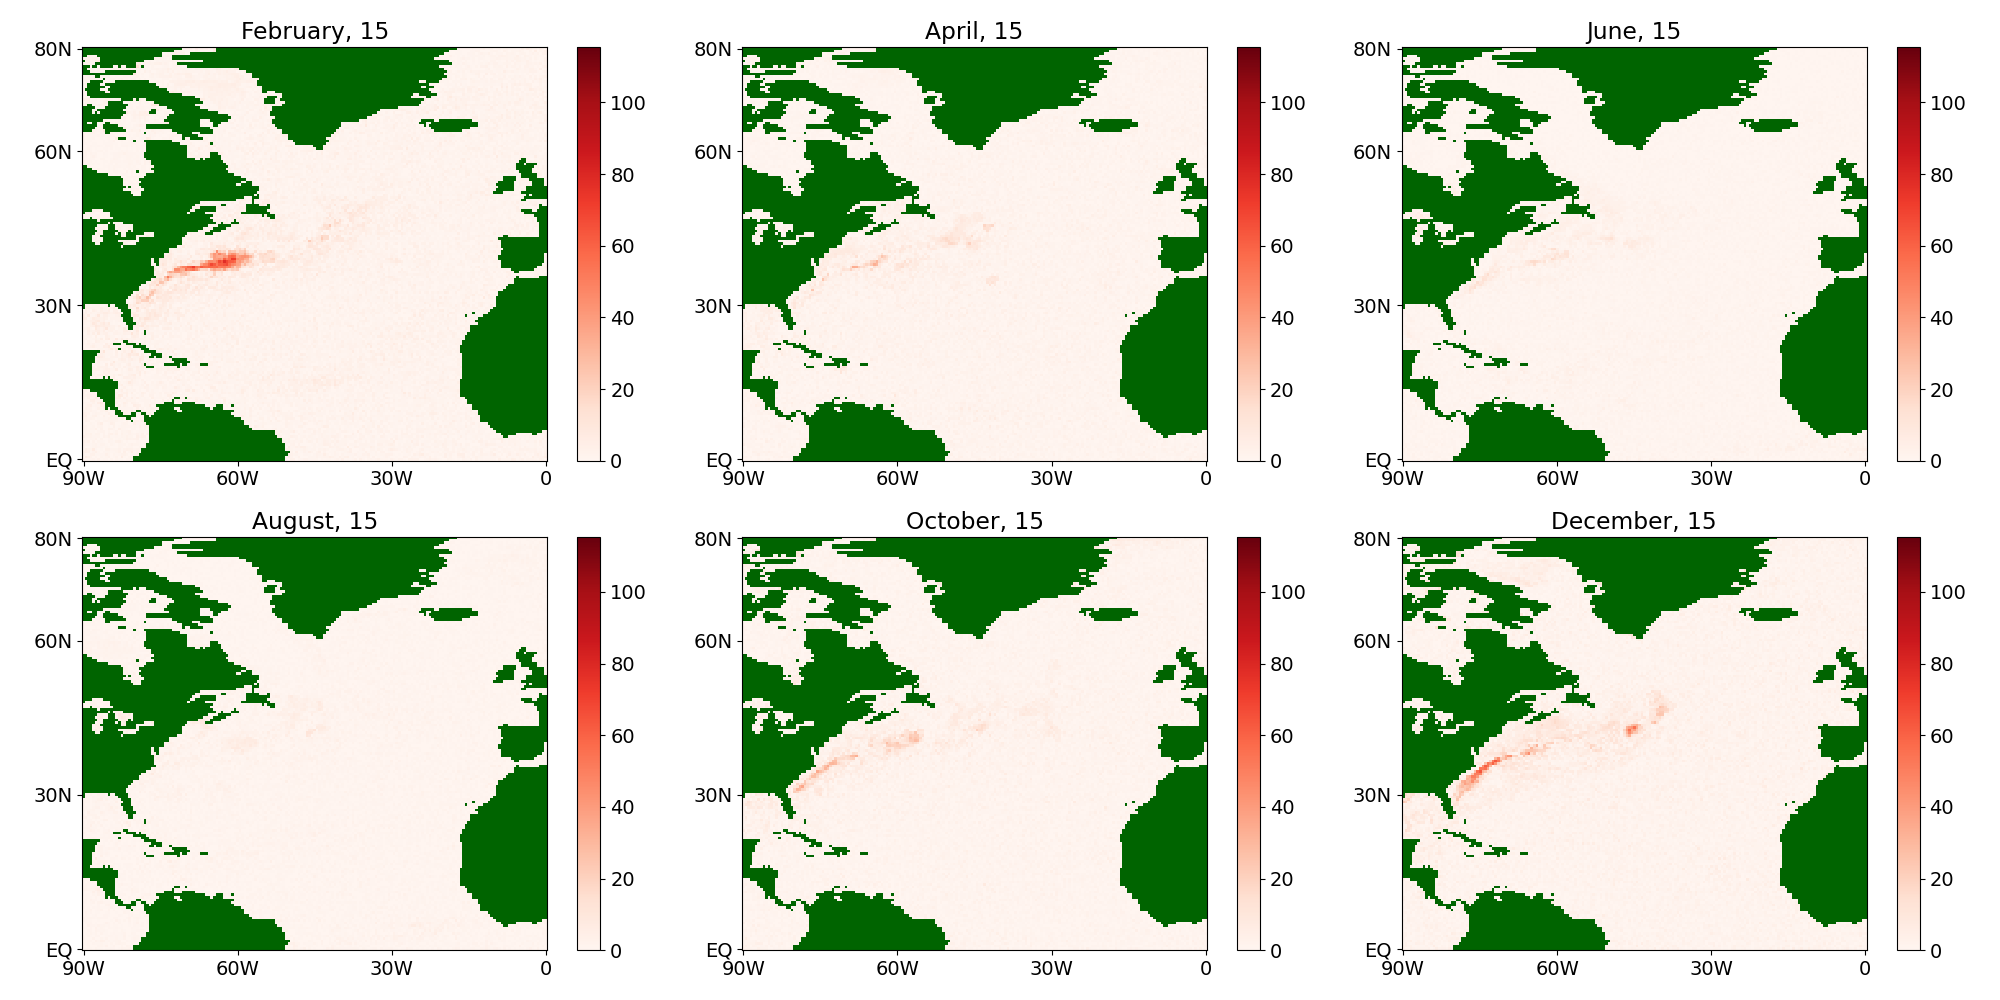
\includegraphics[width=\textwidth]{difference_a_compare_latent}
	\caption{Абсолютная разность оценок коэффициента дрейфа для скрытого потока в течение среднего года за период $1979-2022$ гг.} 
	\label{fig_latent_difference_a}
\end{figure}


\begin{figure}[!h]
	\centering
	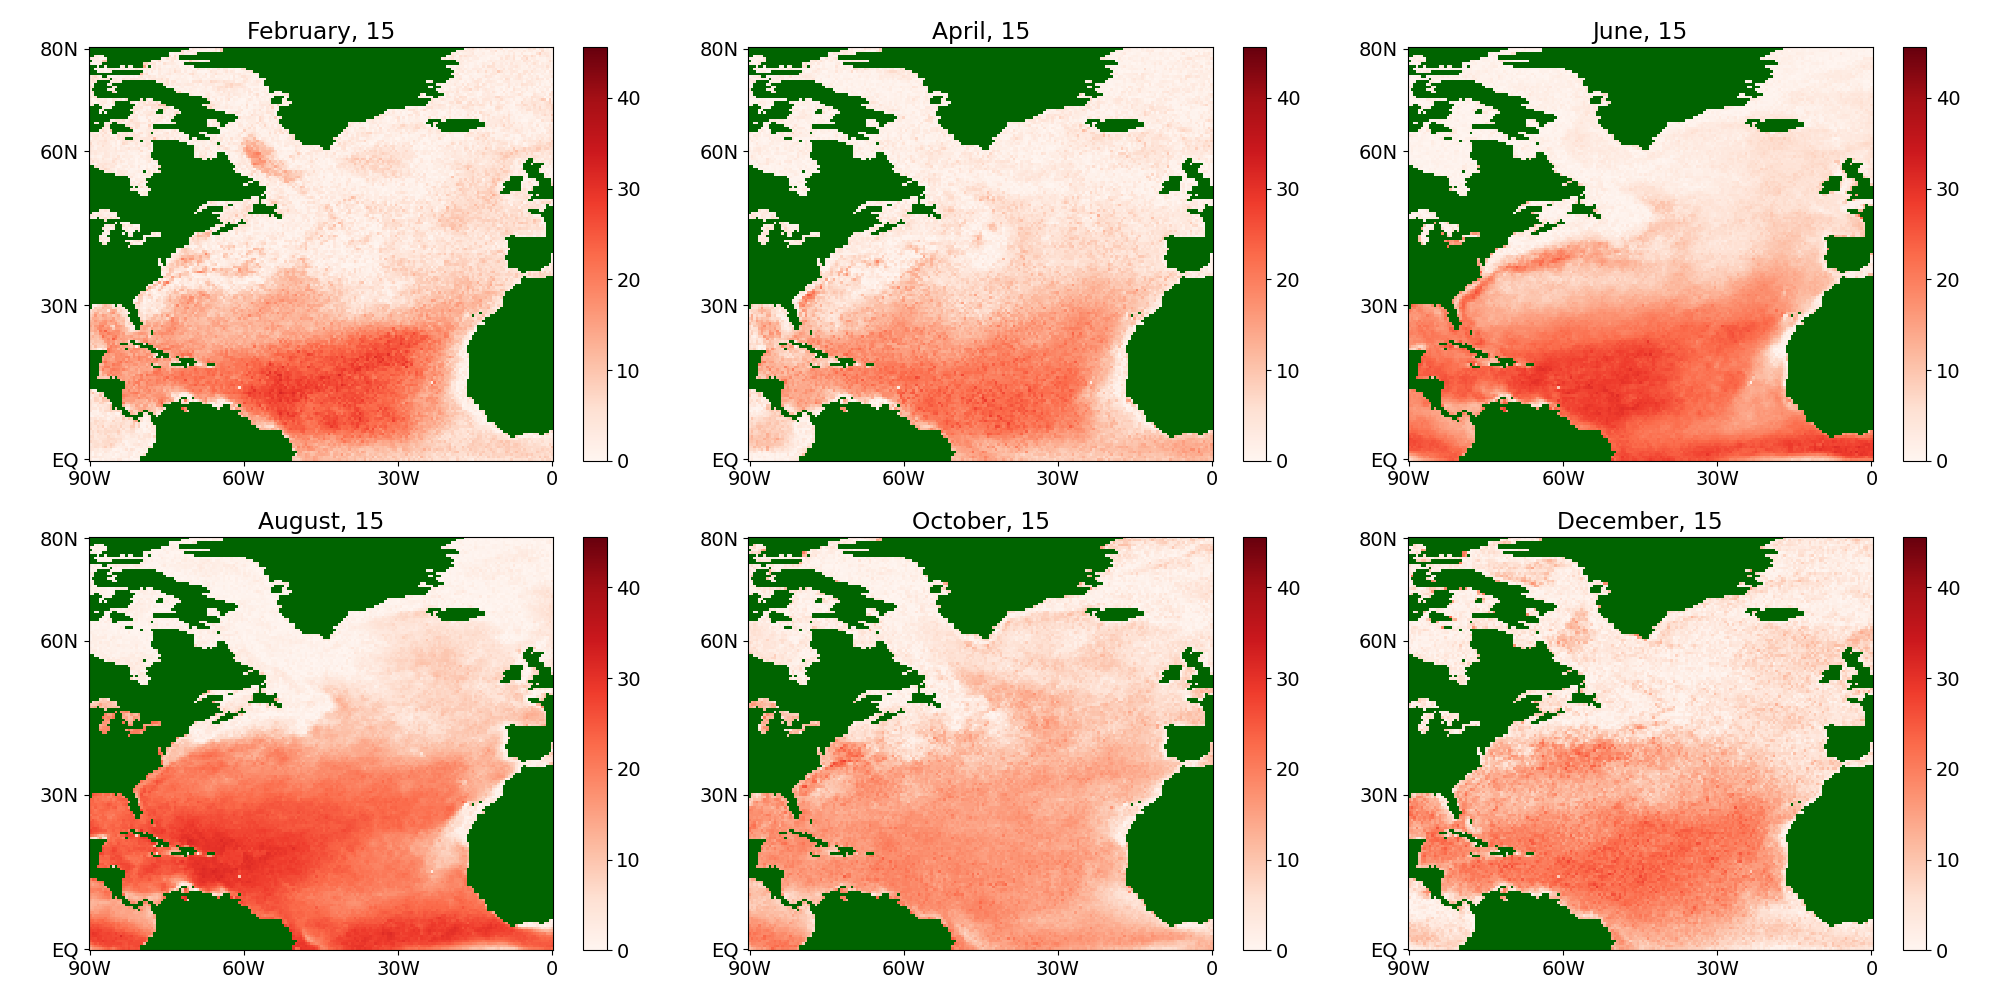
\includegraphics[width=\textwidth]{difference_b_compare_latent}
	\caption{Абсолютная разность оценок коэффициента диффузии для скрытого потока в течение среднего года за период $1979-2022$ гг.} 
	\label{fig_latent_difference_b}
\end{figure}

Для наглядного сравнения результатов, полученных обоими методами сразу для всей Северной Атлантики, значения абсолютных различий оценок в каждой точке полуградусной сетки представлены на рисунках \ref{fig_sensible_difference_a}-\ref{fig_latent_difference_b}. Снова используется формат среднего значения за год.
Что касается коэффициентов дрейфа для потоков обоих типов, то вдоль Гольфстрима наблюдаются некоторые существенные различия в результатах применения методов (см. рисунки \ref{fig_sensible_difference_a} и \ref{fig_latent_difference_a}), в то время как для остальной части карты различия могут проявляться из-за ошибок в расчетах.

В то же время разница между полученными значениями коэффициента диффузии видна гораздо отчетливее (см. рисунки \ref{fig_sensible_difference_b} и \ref{fig_latent_difference_b}), особенно для зимы и весны среднего года в более северных широтах, а также в районе Гольфстрима. Этот факт может быть объяснен следующим образом. В северных широтах существует больше случайных факторов, определяющих взаимодействие океана и атмосферы, из–за большего разброса температур и более сильных ветров, которые в значительной степени определяют возникающие потоки. Это один из наиболее важных аргументов в пользу более точной полупараметрической процедуры оценки (см. раздел \ref{SecSemiparametric}).

В статье представлены исследования по применению полупараметрического метода для восстановления коэффициентов случайного дрейфа $a(t,X)$ и диффузии $b(t,X)$ в СДУ Ито и сравнения этого метода с непараметрическим методом, используя как синтетически сгенерированные данные, так и данные повторного анализа явного и скрытого тепла потоки в Северной Атлантике за период с $1979$ по $2022$ год из базы данных ERA5.
К преимуществам непараметрических процедур относится возможность теоретического доказательства свойств оценок, например, их согласованности, в том числе для многомерного случая. Однако этот метод требует нескольких дополнительных допущений. Процедура полупараметрической реконструкции свободна от них. Необходимо только наличие решения стохастического дифференциального уравнения. Однако этот метод ориентирован на выборки ограниченного объема (окна), что накладывает ограничения на возможность доказательства асимптотических статистических свойств. Однако эмпирическое сравнение обоих методов, приведенное в статье, показывает сходство их результатов, что указывает на возможность использования этих методов для прикладного математического моделирования.

\section{Разложение коэффициента диффузии на собственные вектора}
\subsection{Разложение Карунена-Лоэва}   
\label{SecKarhunen}

Модель~\eqref{Ito} в дискретном виде может быть представлена в виде
\begin{equation}
	\label{discrete_Ito}
	X(t+\Delta t) = a(t,X) \Delta t + b(t,X) (W (t+\Delta t)-W(t))	
\end{equation}
Здесь $X(t)$ и $a(t,X)$ - случайные векторы длиной $N$, $b(t,X)$ - матрица размера $N\times N$, а $W(t)$ -- Винеровский процесс, вектор длины $N$ с независимыми компонентами, который не зависит от процесса $X(t)$. Матрица $b(t,X)$ квадратная, невырожденная, положительно определенная и, следовательно, имеет полный набор собственных векторов $e_1,...,e_N$ и собственных значений $\lambda_1,...,\lambda_N$. Используя стандартный алгебраический метод декомпозиции по базису, из ~\eqref{discrete_Ito} можно получить
\begin{equation}
	\label{decomposition}
	X(t+\Delta t) = X(t) + a(t,X) \Delta t + \sum_{i=1}^N \lambda_i e_i \eta_i
\end{equation}
где $\eta_i= (e_i,W(t+\Delta t)-W(t))$ -- случайная величина и скалярное произведение векторов $e_i$ и $W(t+\Delta t)-W(t)$. Это гауссова случайная величина с нулевым средним значением и дисперсией, равной $\Delta t$, поскольку сумма составляющих вектора $e_i$ определяется однозначно из-за их ортонормированности. Вектор $W (t + \Delta t)-W (t)$ является гауссовым с независимыми компонентами и ковариационной матрицей с ненулевыми диагональными элементами, равными $\Delta t$. Чтобы проанализировать поведение приращений процесса $X(t+\Delta t) - X(t)$, необходимо изучить поведение коэффициента $a(t,X)$ и поведение собственных векторов $e_1,...,e_N$ и собственных значений $\lambda_1,...,\lambda_N$. Этому посвящен следующий раздел.

Мы разбиваем шкалу значений временных рядов за достаточно длительный период времени ($10$ лет) на сегменты, вероятности попадания в которые случайно выбранных значений были бы максимально близки друг к другу. Мы называем этот процесс квантификацией.


\subsection{Собственные значения и векторы}
\label{algorithm}

Алгоритм декомпозиции заключается в следующем:
\begin{itemize}
	\item Рассмотрим два временных ряда $X,Y$ (не обязательно разных, может быть $X \equiv Y$). Их значения зависят от координаты точки сетки (с использованием одномерной проекции) и от рассматриваемого момента времени: $X=X(p,t), Y=Y(p,t)$. 
	\item Давайте разделим весь диапазон значений каждого из рядов на $n_{bins}=100$ непересекающихся и равновероятных (построенных с использованием квантилей) интервалов. Для каждой последующей пары дней $(t,t+dt)$, где $dt$ равняется одному дню, выполняются следующие шаги:
	\begin{itemize}
		\item Инициализируем ковариационную матрицу $B$ размера $n_{bins} \times n_{bins}$.
		
		\item Для каждого интервала с номером $i_1$ $(0 \leqslant i_1 \leqslant n_{bins}-1)$ по первой переменной $X$ и независимо для каждого интервала с номером $j_1$ $(0 \leqslant j_1 \leqslant n_{bins}-1)$ по второй переменной $Y$ выбираются точки первого временного ряда в момент времени $t$, которые попадают в интервал $i_1$, обозначим их через $points_{x1}$ и для второго временного ряда в момент времени $t$, попадающего в интервал с номером $j_1$ ($points_{y1}$).
		
		
		\item Для этих точек вычисляются два вектора:
		\begin{equation*}
			vec_1 = X_{points_{x1},t+dt} - mean(X_{points_{x1},t}),\quad
			vec_2 = Y_{points_{y1},t+dt} - mean(Y_{points_{y1},t}).
		\end{equation*}
		В то же время значения $mean(X[points_{x1},t]$) рассчитаны ранее на основе оценок коэффициента дрейфа $a$.
		
		\item Давайте вычислим сумму произведений всех возможных пар этих двух векторов и присвоим соответствующему элементу матрицы $B$:
		\begin{equation*}
			B_{i_1, j_1} = \sum v_1 \cdot v_2, \quad v_1 \in vec_1, v2 \in vec_2.
		\end{equation*}
		Здесь неявно используется закон полной вероятности. Он требует, чтобы мы учитывали вероятности переходов. Однако, поскольку мы используем равновероятные деления интервалов, вероятности для каждого интервала примерно одинаковы, и различиями между ними можно пренебречь. При этом учитывается размерность задачи, то есть берется матрица между значениями разных (либо одних и тех же) переменных.
		
		\item В случае различных переменных в паре $(X,Y)$ вместо матрицы $B$ рассмотрим матрицу $B^*$, полученную из следующего соотношения: ${B^*}^2= B \cdot B^T$.
		
		
		\item Давайте разложим матрицу $B$ на собственные значения и векторы, отсортировав их в порядке убывания абсолютных значений собственных значений: $\lambda_1,\dots,\lambda_{n_{bins}}$; $v_1,\dots,v_{n_{bins}}$.
		
		\item Рассмотрим пару $(\lambda_i, v_i)$, где $\lambda_i$ - это число (вообще говоря, комплексное), а $v_i$ - одномерный вектор длиной $n_{bins}$ (вообще говоря, комплексный). Собственное значение $\lambda_i$ соответствует второй переменной (временной ряд $Y$), что приводит к следующему правилу построения: 
		
		\item Создадим пустую карту $M$, которая представляет собой матрицу размером $161 \times 181$. Для каждого интервала с номером $j_1$ $(0 \leqslant j_1 \leqslant n_{bins}-1)$ в соответствии со второй переменной $Y$ выполняется поиск точек второй строки в момент времени $t+dt$, попадающих в интервал с номером $j_2$: $points_{y2}$. Давайте присвоим действительную часть соответствующего элемента собственного вектора с номером $j_2$ всем точкам этого множества: $M[points_{y2}] = v_i[j_2]$.
	\end{itemize}
\end{itemize}


\section{Архитектура программного комплекса}
\label{SecSoftware} 
В данном разделе обсуждаются вопросы программной реализации описанных в предыдущем разделе методов с использованием высокопроизводительных вычислений для анализа пространственно-временных данных реаализа. На рисунке~\ref{fig_algo} приведена блок-схема алгоритма статистического оценивания коэффициентов $a(t,x)$ и $b(t,x)$ СДУ Ланжевена~\eqref{Ito}. Величины $t_0$ и $t_1$ соответствуют подряд идущим моментам времени. 

\begin{figure}[!h]
	\centering
	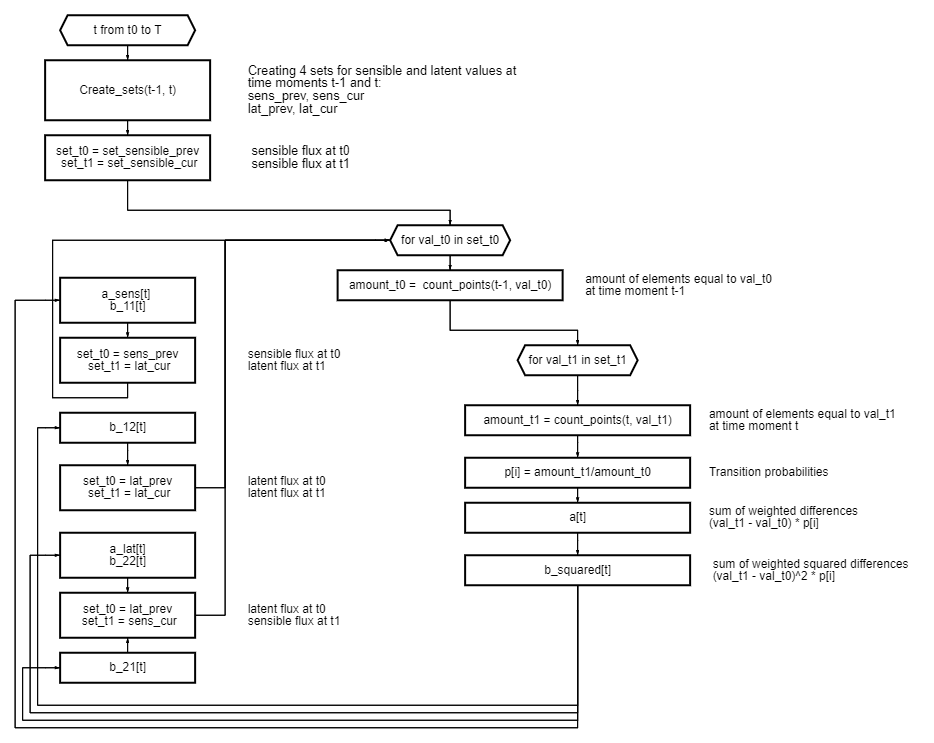
\includegraphics[width=\textwidth]{diagram_eng}
	\caption{Блок-схема алгоритма расчета оценок для коэффициентов $a$ и $b$} \label{fig_algo}
\end{figure}

\begin{figure}[!h]
	\centering
	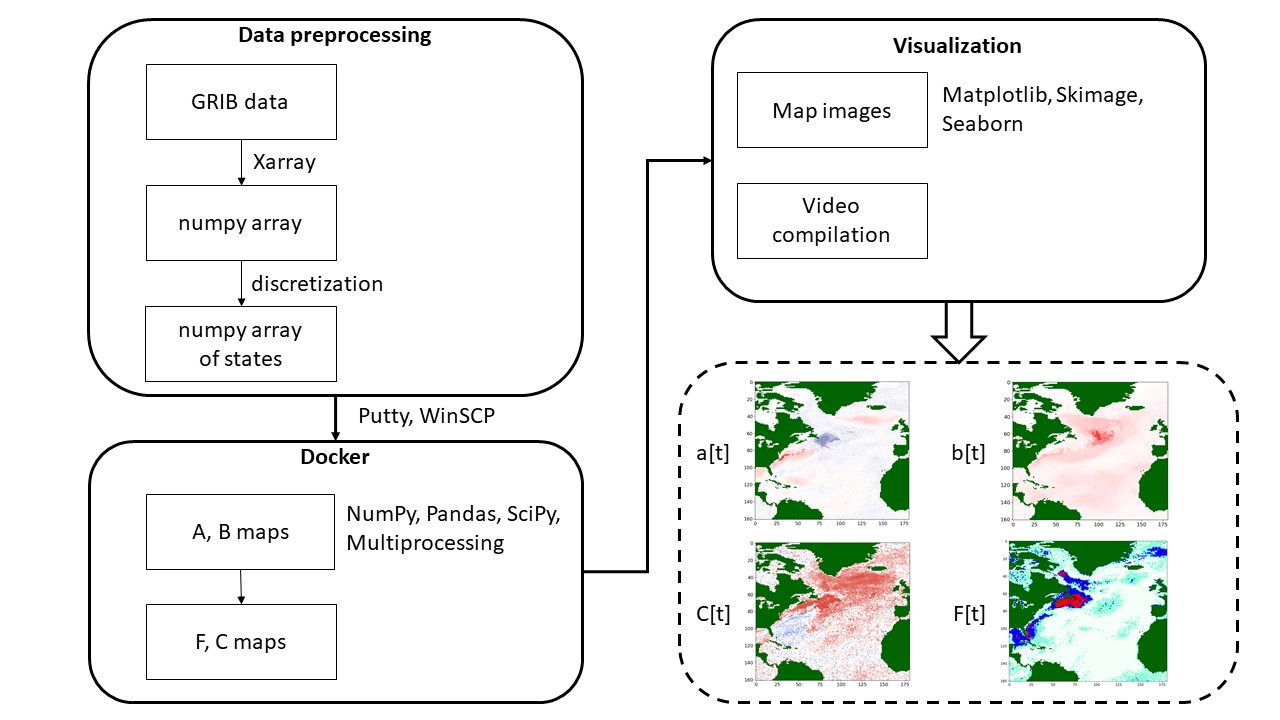
\includegraphics[width=0.99\textwidth]{scheme}
	\caption{Логическое представление архитектуры программного комплекса}\label{fig_app_scheme}
\end{figure}

Оценим вычислительную сложность этого алгоритма. Поскольку на каждом шаге $t \in [t_0,T]$ рассматриваются два момента времени $t_1$ и $t_2$, в которых присутствует вложенный цикл по уникальным значениям двух двумерных массивов, являющихся рассматриваемой сеткой, то сложность алгоритма будет составлять $O(t\times n^2)$, где $n$ – число элементов каждого из массивов. C учетом размеров рассматриваемой сетки, в текущей работе значения этих параметров следующие: $n=161\times181=29141$, $t = [0, 15917]$ - количество дней за рассматриваемый промежуток времени.

На рисунке~\ref{fig_app_scheme} схематично показаны основные структурные компоненты проекта:
\begin{itemize}
	\item Блок \verb"Data prepocessing" содержит программные преобразование формата \verb"GRIB" (используется для хранения и передачи метеорологических данных с привязкой к сетке на двумерной географической карте) в тип данных \verb"NumPy", дискретизация (см. формулы~\eqref{p_formula}--\eqref{b_formula} и соответствующие пояснения к ним в разделе~\ref{SecMethods}).
	\item В блоке \verb"Docker" реализованы вычислительные алгоритмы (см. рисунок~\ref{fig_algo}) для расчет оценок коэффициентов $a$ и $b$, их корреляции и отношения $F$. Используется высокопроизводительный кластер архитектуры Intel x86\_64 (9 узлов на основе серверной платформы \verb"Huawei Server XH620": два \verb"Intel Xeon CPU E5-2683 v4" (2.1 GHz, 16 Core), 512 Gb RAM, 2*10G Ethernet, 2*16G \verb"FibreChannel") и индивидуальная облачная вычислительная среда на основе технологии виртуальной контейнеризации~\cite{peinl2016docker}.
	\item Блок \verb"Visualisation" предназначен для визуализации результатов: для рассматриваемых величин были на локальной машине отрисованы графики в формате карт с последующей сборкой в видеофайлы формата \verb"MP4" продолжительностью около часа каждое.
\end{itemize}

Для программной реализации использованы язык \verb"Python 3.7" и библиотеки \verb"Matplotlib", \verb"NumPy", \verb"Pandas", \verb"SciPy", \verb"Skimage", \verb"Seaborn", \verb"Xarray" (для чтения GRIB-файлов).

На расчет оценок коэффициентов $a$ и $b$ ушло приблизительно $1.5$ дня непрерывных расчетов на кластере (включая накладные расходы), на расчеты $C$ и $F$ -- порядка двух часов. Отрисовка карт и сборка в видео-формат заняла около $3-4$ часов.


\section{Корректность использования модели для данных реанализа}
\label{AppExist}
Решением СДУ вида~\eqref{Ito} является диффузионный процесс с коэффициентом диффузии $b^2(t,X)$ и коэффициентом переноса $a(t,X)$. Случайные коэффициенты $a(t,X)$ и $b(t,X)$ представляют собой условное математическое ожидание и дисперсию приращений потока соответственно:
\begin{gather*}
	a(t,X) = \frac{\E(X(t+dt)-X(t)|X(t)=x)}{dt}, \quad
	% 		\end{equation}
% 		\begin{equation}
	b(t,X) = \frac{\D(X(t+dt)-X(t)|X(t)=x)}{dt}.
\end{gather*}

Предположим, что $a(t,X)$ и $b(t,X)$ –- борелевские функции, определенные при $x \in \R^1$, $t \in [t_0,T]$. Тогда рассматриваемое СДУ эквивалентно следующему уравнению (начальное условие $X(t_0)$ предполагается заданным):
\begin{equation}
	\label{integral_Ito}
	X(t) = X(t_0) + \int_{t_0}^{t} a(s, X(s))ds + \int_{t_0}^{t} b(s, X(s))dW(s).
\end{equation}

Для существования решения уравнения~\eqref{integral_Ito} для некоторого $K$ необходимо~\cite{Skorohod} выполнение условий вида:
\begin{enumerate}
	\item для всех $x$ и $y \in \R^1$: 
	% 			\begin{equation*}
		$|a(t,x)-a(t,y)|+|b(t,x)-b(t,y)| \leqslant K|x-y|$,
		% 			\end{equation*}
	\item для всех $x \in \R^1$: 
	% 			\begin{equation*}\
		$|a(t,x)|^2+|b(t,x)|^2 \leqslant K(1+x^2)$.
		% 			\end{equation*}
\end{enumerate}

Причем если при этом $X_1 (t)$ и $X_2(t)$ -– два непрерывных решения уравнения \ref{integral_Ito}, то они неразличимы.
% 		\begin{equation*}
	% 			\P \left\lbrace \sup_{t_0 \leqslant t \leqslant T} |X_1(t) - X_2(t)| > 0 \right\rbrace = 0.
	% 		\end{equation*}
% 		Более того, при условиях этой теоремы решение уравнения~\ref{integral_Ito} будет процессом Маркова, вероятности перехода которого определяются соотношением:
% 		\begin{equation*}
	% 			P(t,x,s,A)= P\left\lbrace X_(t,x) (s) \in A\right\rbrace 
	% 		\end{equation*}

Проверим выполнение этих условий для анализируемых данных, а именно -- найдем оценку константы $K$. Для неравенства из первого пункта естественным образом будем рассматривать случай $x \ne y$. Имеем:
% 		Оценим константу $K$ в этом неравенстве отдельно для каждого потока следующим образом: найдем минимум выражения $|x-y|$ при $x \ne y$ для всех значений потоков $x$ и $y$, имеющихся в данных. Затем для каждого $t \in [t_0,T]$ максимизируем разности $|a(t,x)-a(t,y)|+|b(t,x)-b(t,y)|$ и возьмем максимум по $t$. Тогда для 
\begin{equation*}
	K \geqslant \frac{\max(|a(t,x)-a(t,y)|+|b(t,x)-b(t,y)|)}{\min(|x-y|)}.
\end{equation*}
% 	первое неравенство будет выполнено для рассматриваемого типа потока. Для того, чтобы получить универсальную константу для обоих типов потоков, возьмем максимум из двух оценок.

Для второго неравенства, учитывая, что $(1+x^2 )\geqslant 1$, получим:
\begin{equation*}
	K \geqslant \max\limits_{x \in \R^1, t \in [t_0,T]}(|a(t,x)|^2 + |b(t,x)|^2).
\end{equation*}
% 	где максимум берется по всем присутствующих в данных значениям потока $x$ и при всех $t \in [t_0,T]$.

В данных присутствует небольшое количество выбросов, которые могут в несколько раз превосходить типичные значения коэффициентов. Для определения коэффцициентов в неравенствах они могут быть исключены: в качестве максимума для каждого типа потока выбирается квантиль порядка $0.97$, а в качестве минимума – $0.03$. 
В силу объема данных вычисление квантилей на всем промежутке времени одновременно затруднительно, поэтому квантили считались на отрезках по $1000$ дней, а затем в качестве верхней квантили брался максимум из них на каждом отрезке, а в качестве нижней –- минимум. Кроме того, введем условие отделимости от $0$ разности $x-y$, эмпирически выбран порог $0.1$.

С учетом введенных ограничений были получены следующие значения верхних и нижних квантилей для $a$ и $b$: $b_{up} = 148.02$, $b_{low} = 0$ (из физического смысла, случаи комплексных $b$ и потому отрицательных значений не рассматриваются), $a_{up} = 40.77$, $a_{low} = -32.02$. При таких введенных ограничениях получаем оценку на K для первого неравенства	$K_1 \geqslant 2209$ и для второго -- 	$K_2 \geqslant 23572$. 	Таким образом, необходимое конечное значение $K$ существует, гарантируя корректность применяемой в работе математической модели.

% 	\section{Вычислительная сложность алгоритма оценивания коэффициентов СДУ}
% 	\section{Алгоритм оценивания коэффициентов СДУ Ланжевена}
% 	\label{AppAlgorithm}
% 		На рисунке~\ref{fig_algo} приведена блок-схема алгоритма статистического оценивания коэффициентов $a(t,x)$ и $b(t,x)$ СДУ Ито~\eqref{Ito}. Величины $t_0$ и $t_1$ соответствуют двум подряд идущим моментам времени. 

% 		\begin{figure}[h!]
	% 			\center{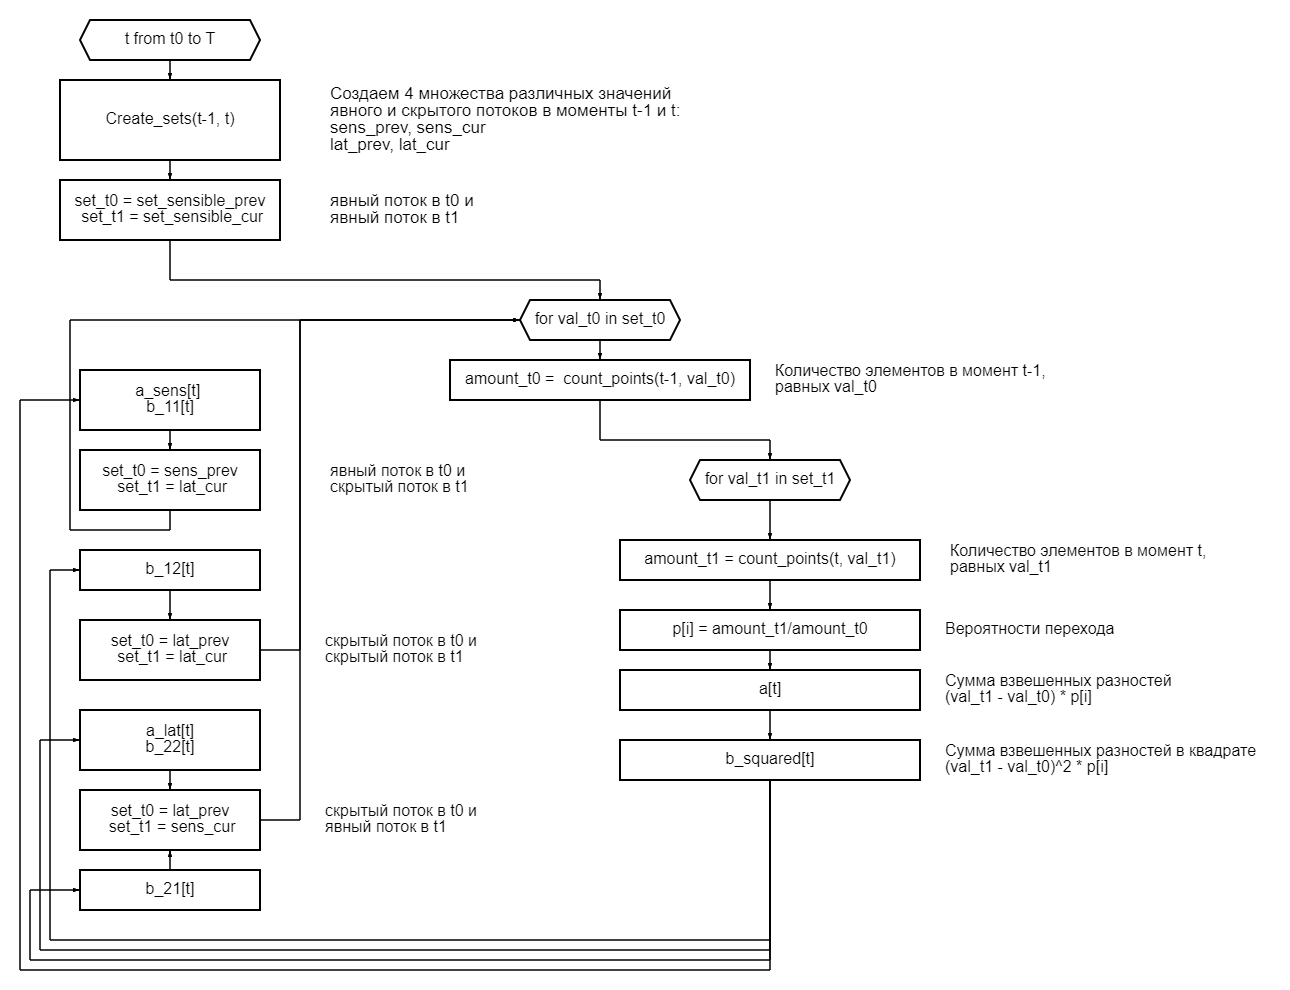
\includegraphics[width=\textwidth]{diagram}}
	% 			\caption{Блок-схема алгоритма расчета оценок для коэффициентов $a$ и $b$} \label{fig_algo}
	% 		\end{figure}

% 		Оценим вычислительную сложность этого алгоритма. Поскольку на каждом шаге $t \in [t_0,T]$ рассматриваются два момента времени $t_1$ и $t_2$, в которых присутствует вложенный цикл по уникальным значениям двух двумерных массивов, являющихся рассматриваемой сеткой, то сложность алгоритма будет составлять $O(t\times n^2)$, где $n$ – число элементов каждого из массивов. C учетом размеров рассматриваемой сетки, в текущей работе значения этих параметров следующие: $n=161\times181=29141$, $t = [0, 15917]$ - количество дней за рассматриваемый промежуток времени.

% 		Расчет оценок коэффициентов $a$ и $b$, их корреляции и отношение $F$ выполнялись на высокопроизводительном кластере в индивидуальной вычислительной среде на основе технологии виртуальной контейнеризации docker. После выполнения всех расчетов для рассматриваемых величин были на локальной машине отрисованы графики в формате карт с последующей сборкой в видеофайлы формата mp4 продолжительностью около часа каждое.  
%         Программная реализация была выполнена на языке Python 3.7 с использованием библиотек Matplotlib, NumPy, Pandas, SciPy, Skimage, Seaborn, Xarray (для чтения grib-файлов) и др.

% 		На рисунке \ref{fig_app_scheme} схематично показаны основные структурные компоненты проекта: программные преобразование формата grib в numpy, дискретизация, расчет оценок коэффициентов, визуализация результатов.

% 		\begin{figure}[h!]
	% 			\center{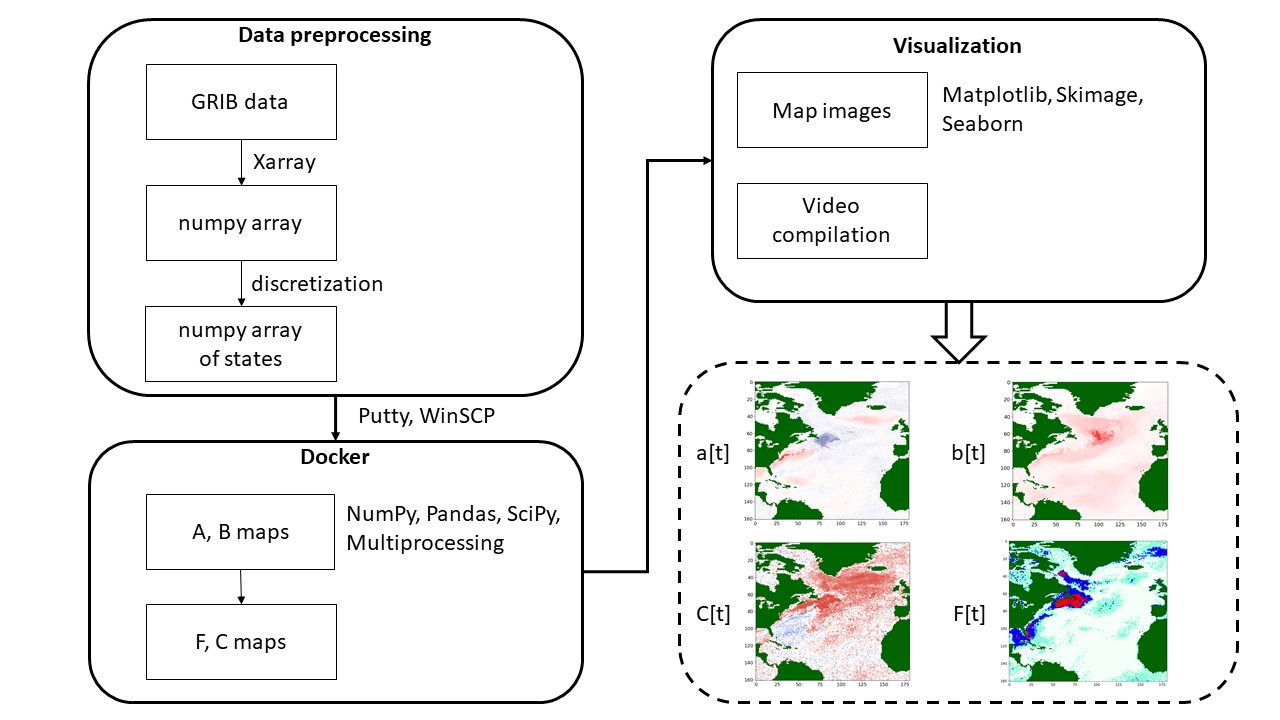
\includegraphics[width=\textwidth]{scheme}}
	% 			\caption{Логическое представление архитектуры программного комплекса}\label{fig_app_scheme}
	% 		\end{figure}


%     \section{Программная реализация}
% 		Исходные данные измерений явного и скрытого потока представляли собой 2 файла формата grib из открытой базы ERA5 (https://www.ecmwf.int/en/forecasts/datasets/reanalysis-datasets/era5), каждый из которых содержал в себе ежедневные измерения с шагом в $6$ часов за период 01.01.1979 -- 31.07.2022 на сетке с шагом в $0.5$ градуса со значениями широты в пределах $[-90, 0]$ и долготы в интервале $[0, 80]$ градусов. Для расчета коэффициентов данные были перегруппированы в numpy-массивы по десятилетиям (1979-1989гг., 1989-1999гг., 1999-2009гг., 2009-2019гг., 2019-2022гг.) с уменьшением размерности сетки до 1 градуса. Затем для выполнения расчетов с шагом в $1$ день данные были усреднены по $4$ подряд идущих измерения, за каждый день. Для выполнения расчетов оценок коэффициентов $a$ и $b$ данные предварительно дополнительно подвергались (дискредитации :D) дискретизации, как подробно описано в разделе~\ref{quantification}. Благодаря свойствам марковости рассматриваемых процессов стало возможно реализовать параллельный расчет на нескольких процессах-нитях с последующей сборкой результатов и обработкой границ интервалов родительским процессом, где параллелизм выполнялся по координате времени. 

%         % 		The research was carried out using the infrastructure of the Shared Research Facilities «High Performance Computing and Big Data» (CKP «Informatics») of FRC CSC RAS (Moscow).
% 		Работа выполнялась с использованием инфраструктуры Центра коллективного пользования «Высокопроизводительные вычисления и большие данные» (ЦКП «Информатика») ФИЦ ИУ РАН (г. Москва). Расчет оценок коэффициентов $a$ и $b$, их корреляции и отношение $F$ выполнялись на кластере в индивидуальной вычислительной среде на основе технологии виртуальной контейнеризации docker. После выполнения всех расчетов для рассматриваемых величин были на локальной машине отрисованы графики в формате карт с последующей сборкой в видеофайлы формата mp4 продолжительностью около часа каждое.  
% 		Программная реализация была выполнена на языке Python 3.7 с использованием библиотек NumPy, Pandas, SciPy, Skimage, Seaborn, Xarray (для чтения grib-файлов) и др.       
           % Глава 1
\chapter{Анализ потоков тепла на основе динамико-стохастической модели}
\label{SecAnalysis}
В данной главе рассматривается взаимное влияние этих величин, выявляются области преобладания диффузионной составляющей над дрейфовой. Поскольку параметр диффузии является матричной величиной, эта матрица векторизована с использованием разложения на собственные векторы и значения. Физический смысл этих разложений и результирующие пространственные структуры, а также их изменения во времени соответствуют системе океанских течений в атлантической меридиональной опрокидывающей циркуляции~\cite{Caesar2018} и крупномасштабным тепловым волнам.

Рассмотрим результаты, полученные с использованием описанных в главе~\ref{SecMethods} методов и программных решений из раздела~\ref{SecSoftware}. Рассматриваются как точечные оценки случайных коэффициентов $a(t,X)$ и $b(t, X)$ в СДУ Ито~\eqref{Ito}, так и взаимосвязи между ними за почти $44$ года наблюдений. Расчеты проведны для различных осреднений (сутки, месяц и т.д.), результаты отображаются на динамических картах\footnote{Пятиминутные демонстрационные видео с полученными за $43.5$ года картами доступны по ссылке:~\url{maps_example.video.ru}} для рассматриваемого временного интервала для всех изучаемых точек акватории Северной Атлантики. Ниже приведены примеры построенных карт для некоторых выбранных моментов времени, демонстрирующие описываемые эффекты.


\section{Коэффициент сноса}
Рассмотрим сначала оценки для коэффициента сноса $a(t,X)$, то есть динамической составляющей процесса.
При визуализации (см. рисунок~\ref{fig_ab_mean_year}) используется цветовая шкала, аналогичная потокам на рисунке~\ref{fig_flux_example}: цвет меняется от темно-синего при отрицательных значениях полученных оценок до белого при значениях, близких к нулю, и далее до темно-красного при увеличении положительных значений. Яркость цвета в конкретной точке соответствует удаленности значения от нуля. Темно-зеленым цветом обозначены участки суши.

По результатам анализа многолетних данных установлено, что максимумы динамической составляющей соответствуют направлению основного потока Гольфстрима. Типичной для коэффициента сноса является ситуация, в которой в фиксированной точке направление движения потока меняется на противоположное быстрее, чем за сутки. На динамических картах это выражается в изменении ее раскраски с синего цвета на красный (или наоборот) при отрисовке двух подряд идущих дней.

В период с октября по апрель наблюдаются более высокие абсолютные значения оценок (что соответствует более ярким цветам на картах), в то время как в летние месяцы значения носят более умеренный характер. В таблице~\ref{table_quantiles_a} представлены диапазоны между квантилями уровня $0.1$ и $0.9$ в летний и зимний периоды для полученных оценок коэффициента сноса двух типов потоков - $a_1$ и $a_2$, соответственно. 

\begin{table}[h!]
	\centering
	\caption{Диапазоны значений в летние и зимние периоды между квантилями уровня $0.1$ и $0.9$ для $a_1$ и $a_2$}
	\begin{tabular}{|c|c|c|c|c|}
		\hline
		Период & 1979-1989гг. &  1989-1999гг. & 1999-2009гг. & 2009-2019гг.\\
		\hline
		$a_1$, лето & $[-3.8, 4.1]$ & $[-4.1, 4.1]$ & $[-4.1, 4.3]$ & $[-4.1, 4.3]$\\ 
		\hline
		$a_1$, зима & $[-11.2, 10.2]$ & $[-12.2, 10.5]$ & $[-11.6, 10.9]$ & $[-10.2, 8.9]$\\ 
		\hline
		$a_2$, лето & $[-13.1, 13.8]$ & $[-13.5, 13.8]$ & $[-14.1, 14.8]$ & $[-14.5, 15.5]$\\
		\hline
		$a_2$, зима & $[-23.9, 24.7]$ & $[-24.9, 25.6]$ & $[-24.1, 26.2]$ & $[-24.6, 25.4]$\\ 
		\hline
	\end{tabular}
	\label{table_quantiles_a}
\end{table}

Для наглядной демонстрации этого эффекта на рисунке~\ref{fig_ab_mean_year} изображены оценки коэффициента сноса по акватории за так называемый средний год: для $6$ выбранных дней за год в различные сезоны ($15$ февраля, апреля, июня, августа, октября и декабря) для явного (рисунок~\ref{fig_ab_mean_year}a)) и скрытого (рисунок~\ref{fig_ab_mean_year}b)) потоков усредняются наблюдения за $43$ анализируемых года ($1979$--$2021$ гг.). Полные данные за $2022$ год на момент подготовки текста еще не были доступны, поэтому в данном случае в расчетах не использовались.

\begin{figure}[h!]
	\center{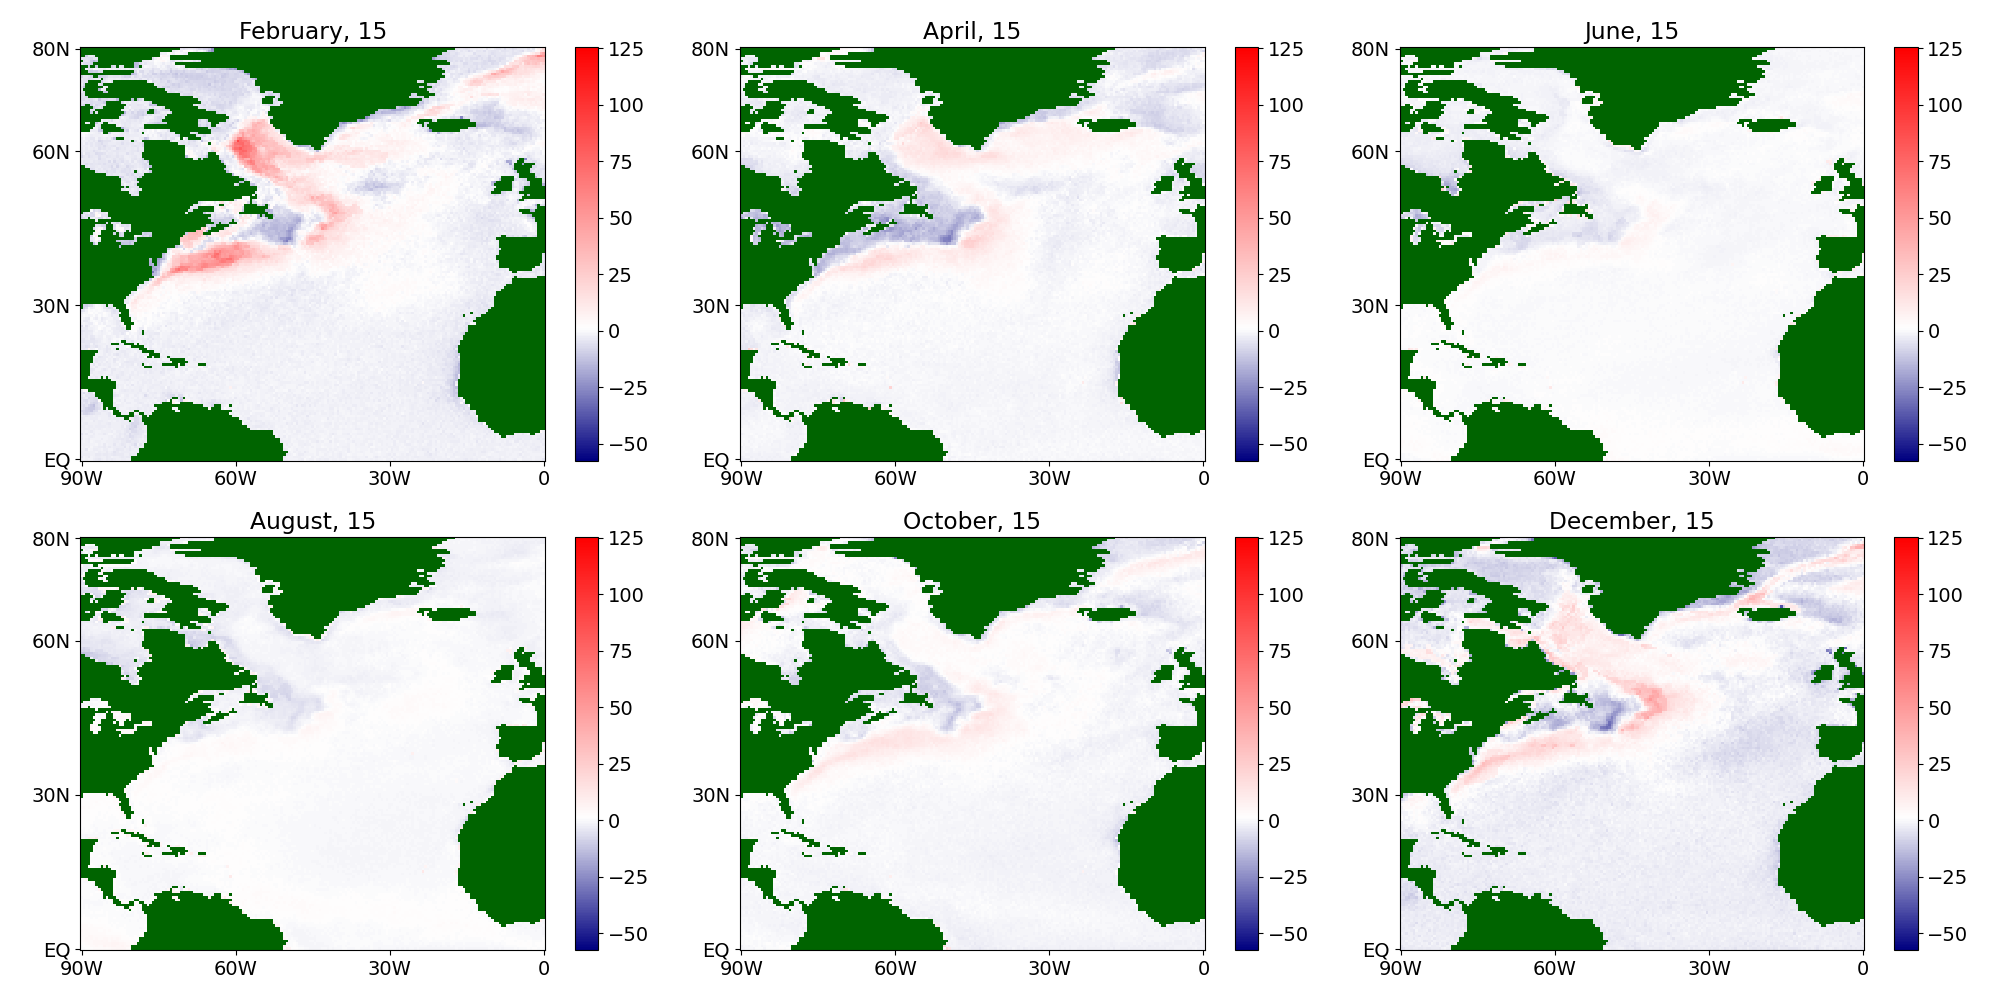
\includegraphics[width=\textwidth]{A_sens_mean_year}}\\
	a)
	\center{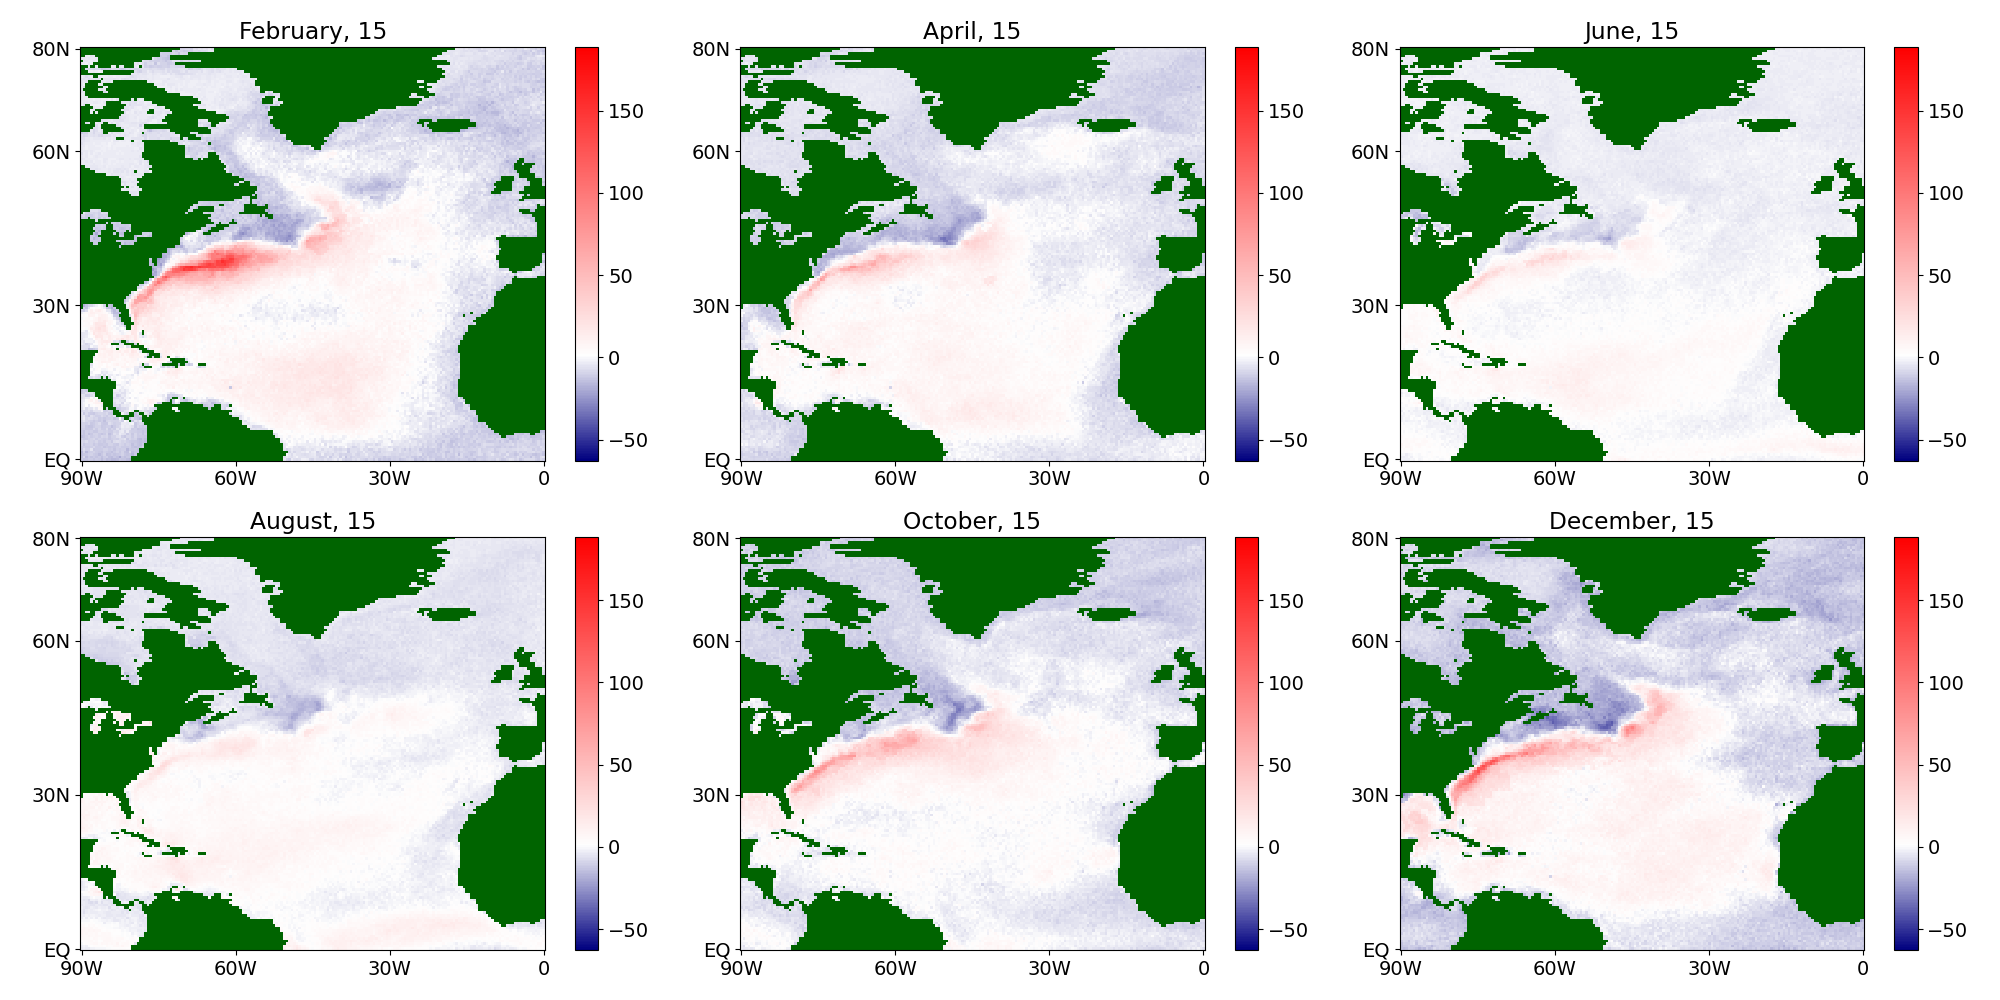
\includegraphics[width=\textwidth]{A_lat_mean_year}}\\
	b)
	
	\caption{Значения коэффициента сноса для явного (a) и скрытого (b) потоков в течение среднего года, $1979$--$2021$ гг.} \label{fig_ab_mean_year}
\end{figure}

С точки зрения геофизики, эти районы показывают преобладание явного потока тепла (рис.~\ref{fig_ab_mean_year}a), то есть непосредственно разности температур вода--воздух и их динамику во времени с преимущественным направлением внутри океана: в зимние месяцы хорошо видна зона основного течения Гольфстрима. Наоборот, поток из атмосферы (нагрев океана) наблюдается в районе Лабрадорского течения. В переходный период (апрель--май) зона передачи тепла в атмосферу уменьшается (температуры выравниваются), а холодное Лабрадорское течение по-прежнему забирает тепло из атмосферы, имея минимальную динамику вдоль Атлантического побережья. В летние месяцы все процессы выравниваются, и наблюдаемые явления возобновляются только в ноябре--декабре. При этом <<холодная>> зона в районе Лабрадора остается, хотя контраст с окружающим воздухом уменьшается.

Все эти процессы гораздо заметнее для скрытых потоков (рис~\ref{fig_ab_mean_year}b), для которых передача тепла (влаги) из атмосферы в океан в северных широтах происходит практически на протяжении всего года, так как нагретая и влажная атмосфера при столкновении с относительно холодным океаном сохраняет стационарное состояние в обширных областях. Только вдоль Северо-Атлантического течения и Скандинавского побережья прослеживается слабый положительный скрытый поток. 

\section{Коэффициент диффузии}
Для матричного коэффициента диффузии $b(t,X)$ также были построены оценки за весь рассматриваемый период с шагом в $1$ день. Пример для одного из дней февраля $2022$ года приведен на рисунке~\ref{fig_b_example}. Расположение оценок на картах соответствует структуре матрицы $b$, приведенной в формуле~\eqref{b_coeff}: левый верхний квадрат отвечает элементу $b_{11}(t,X)$ и т.д. Для отображения значений на карте используется красный цвет различной интенсивности.

\begin{figure}[h!]
	\center{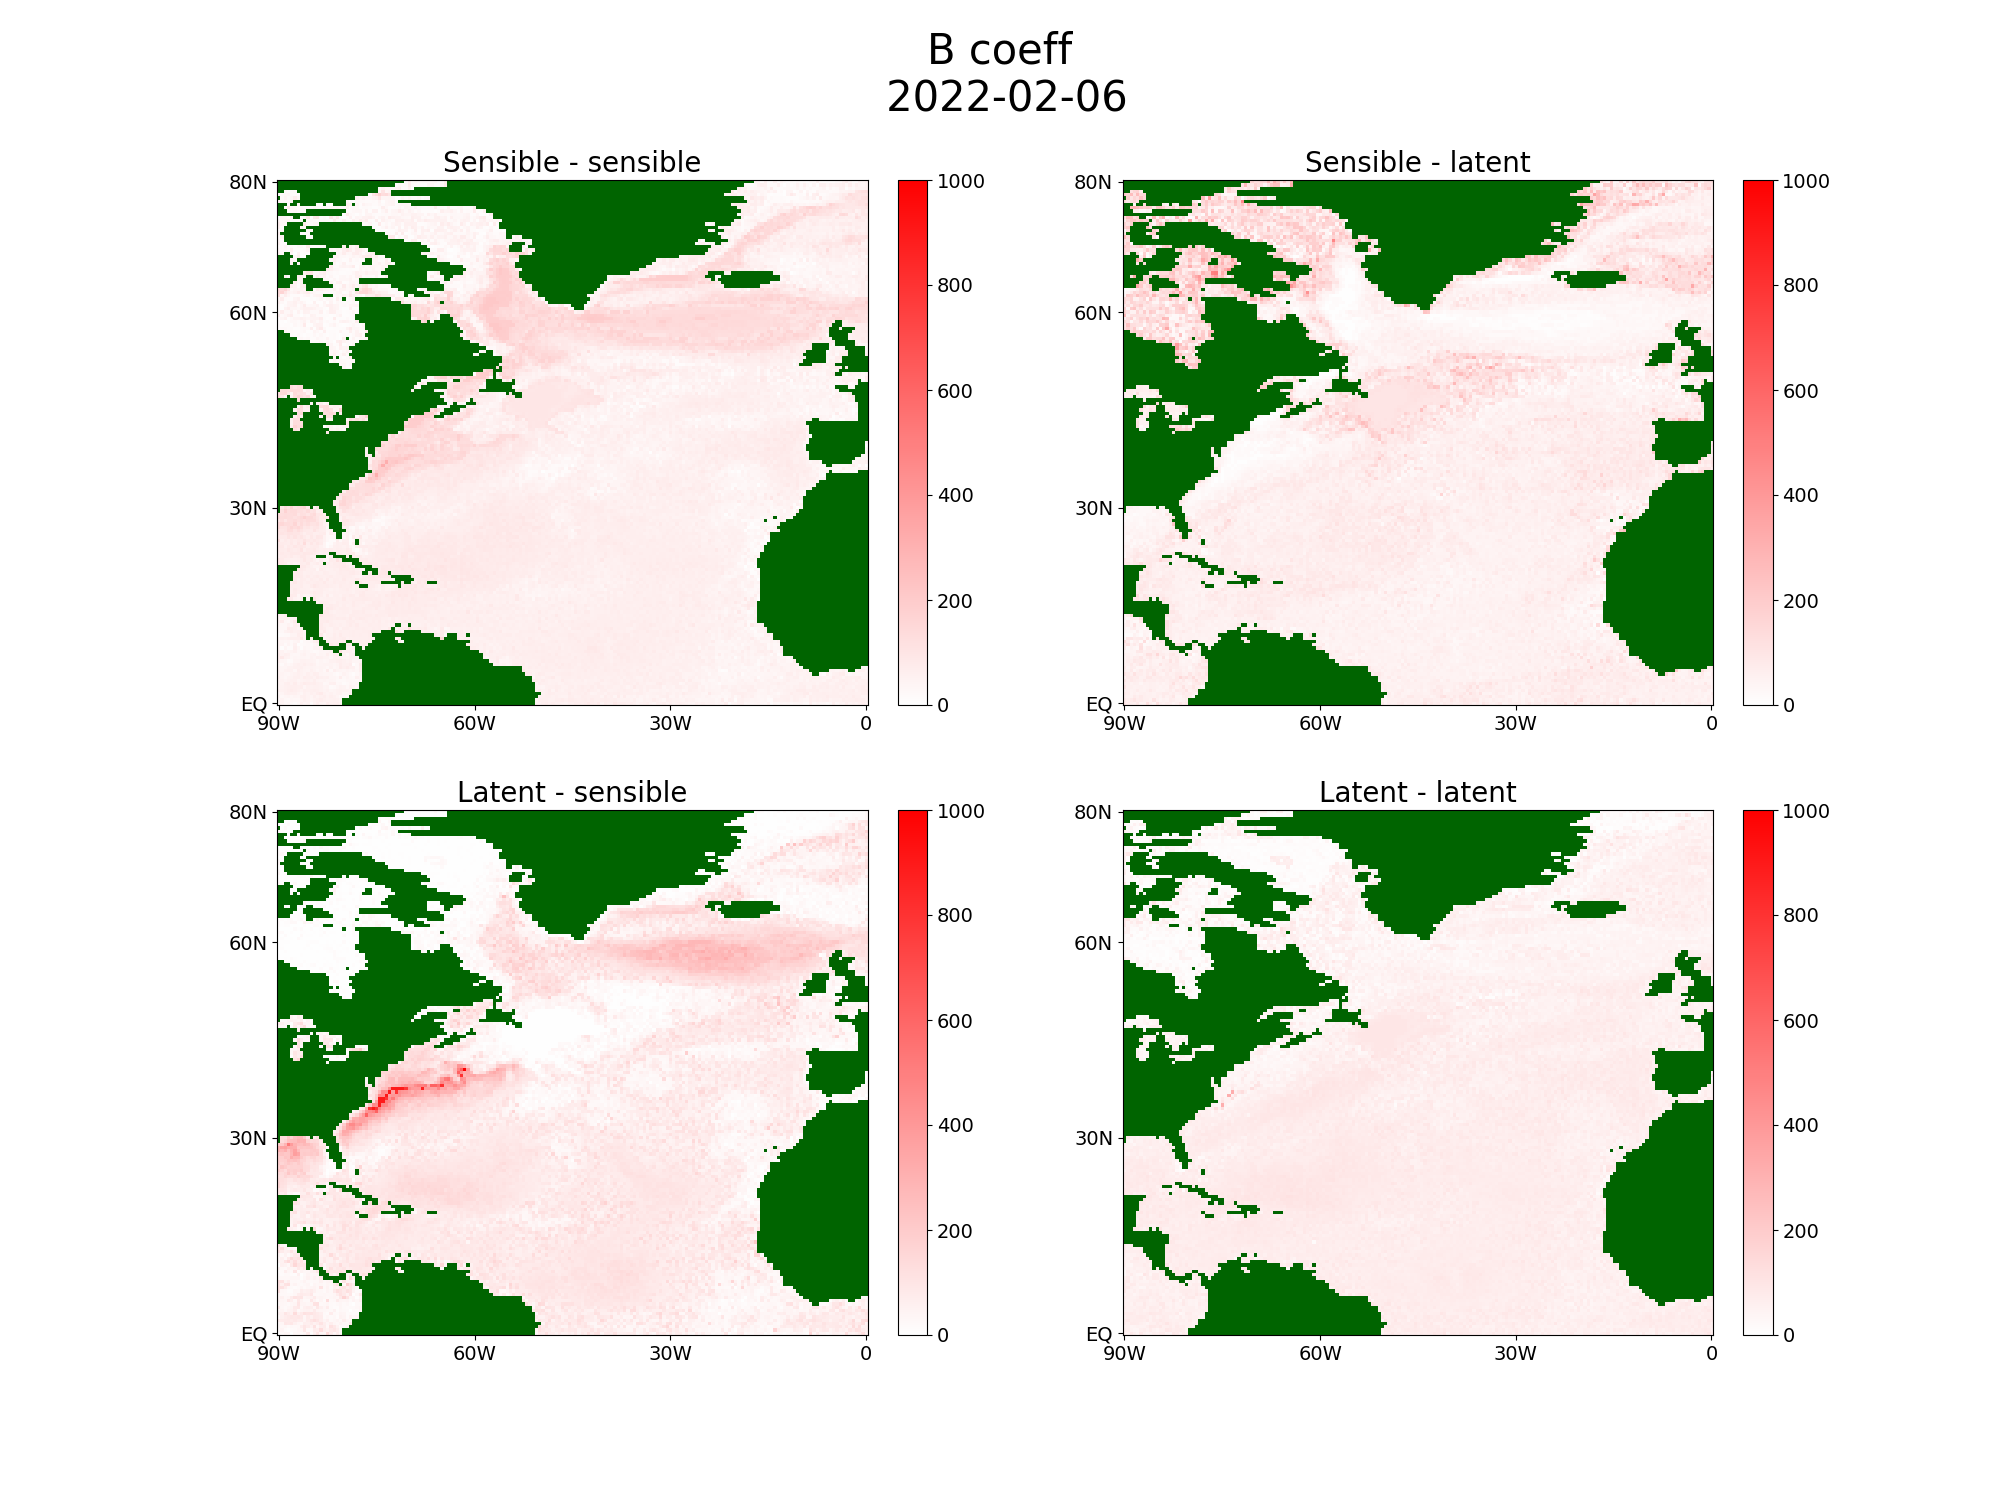
\includegraphics[width=0.8\textwidth]{B_15742}}
	\caption{Пример оценок коэффициента диффузии} \label{fig_b_example}
\end{figure}

% 	Цветовая шкала меняется от $0$ (белый цвет) и далее используется красный диапазон для положительных значений.
% 	Отрицательные значения, напомним, встречались при взятии матричного корня на побочной диагонали, как комплексные значения, для которых сохранялись только действительная часть числа.
Яркость цвета в конкретной точке соответствует удаленности значения от нуля. При этом на цветовой шкале максимум выбран равным $1000$ для максимальной наглядности. Более высокие значения наблюдались менее чем в $0.1\%$ случаев, поэтому во избежание излишнего размывания цветовых диапазонов при визуализации обозначались максимальным допустимым значением из диапазона и соответствующим цветом. Темно-зеленым цветом обозначена суша. На рисунке~\ref{fig_b_mean_year} изображены оценки $b_{11}(t,X)$ (рис.~\ref{fig_b_mean_year}a)) и $b_{22}(t,X)$ (рис.~\ref{fig_b_mean_year}b)) в выбранные дни за средний год.


\begin{figure}[!h]
	\center{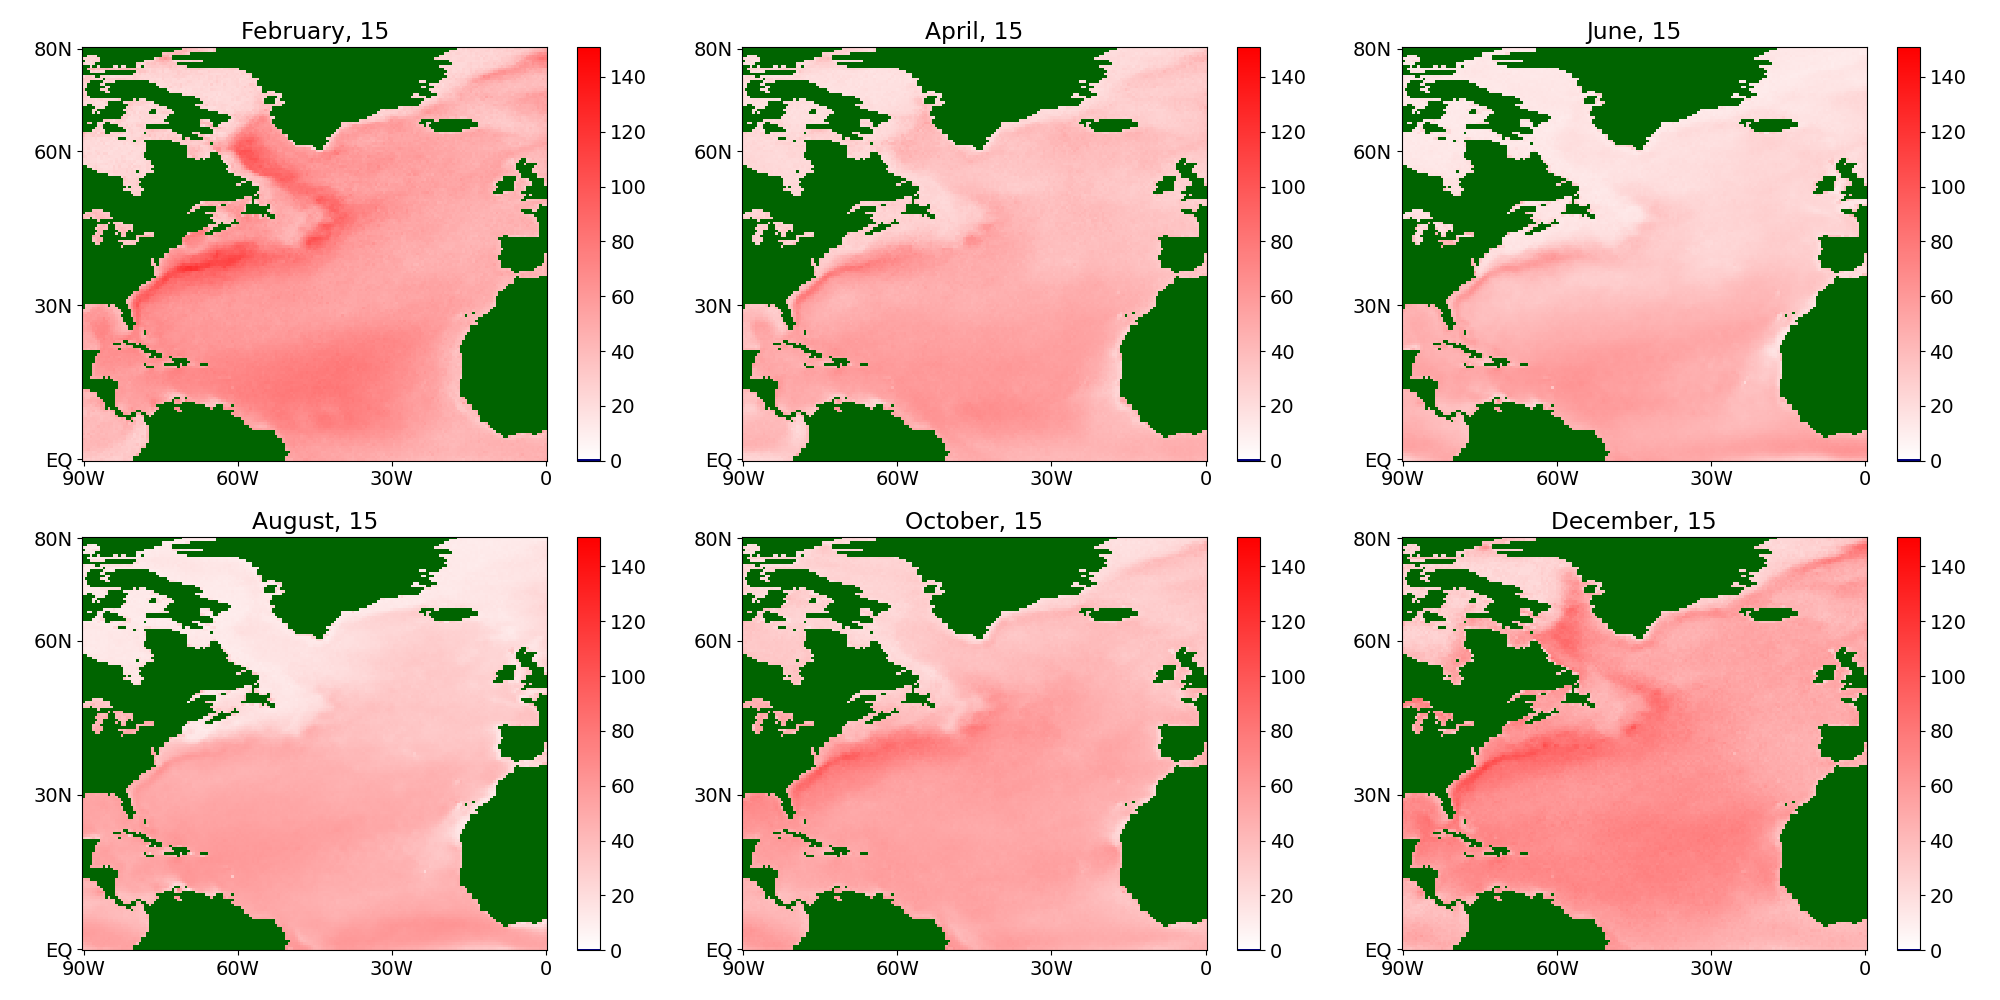
\includegraphics[width=\textwidth]{B11_mean_year}}\\
	a)
	\center{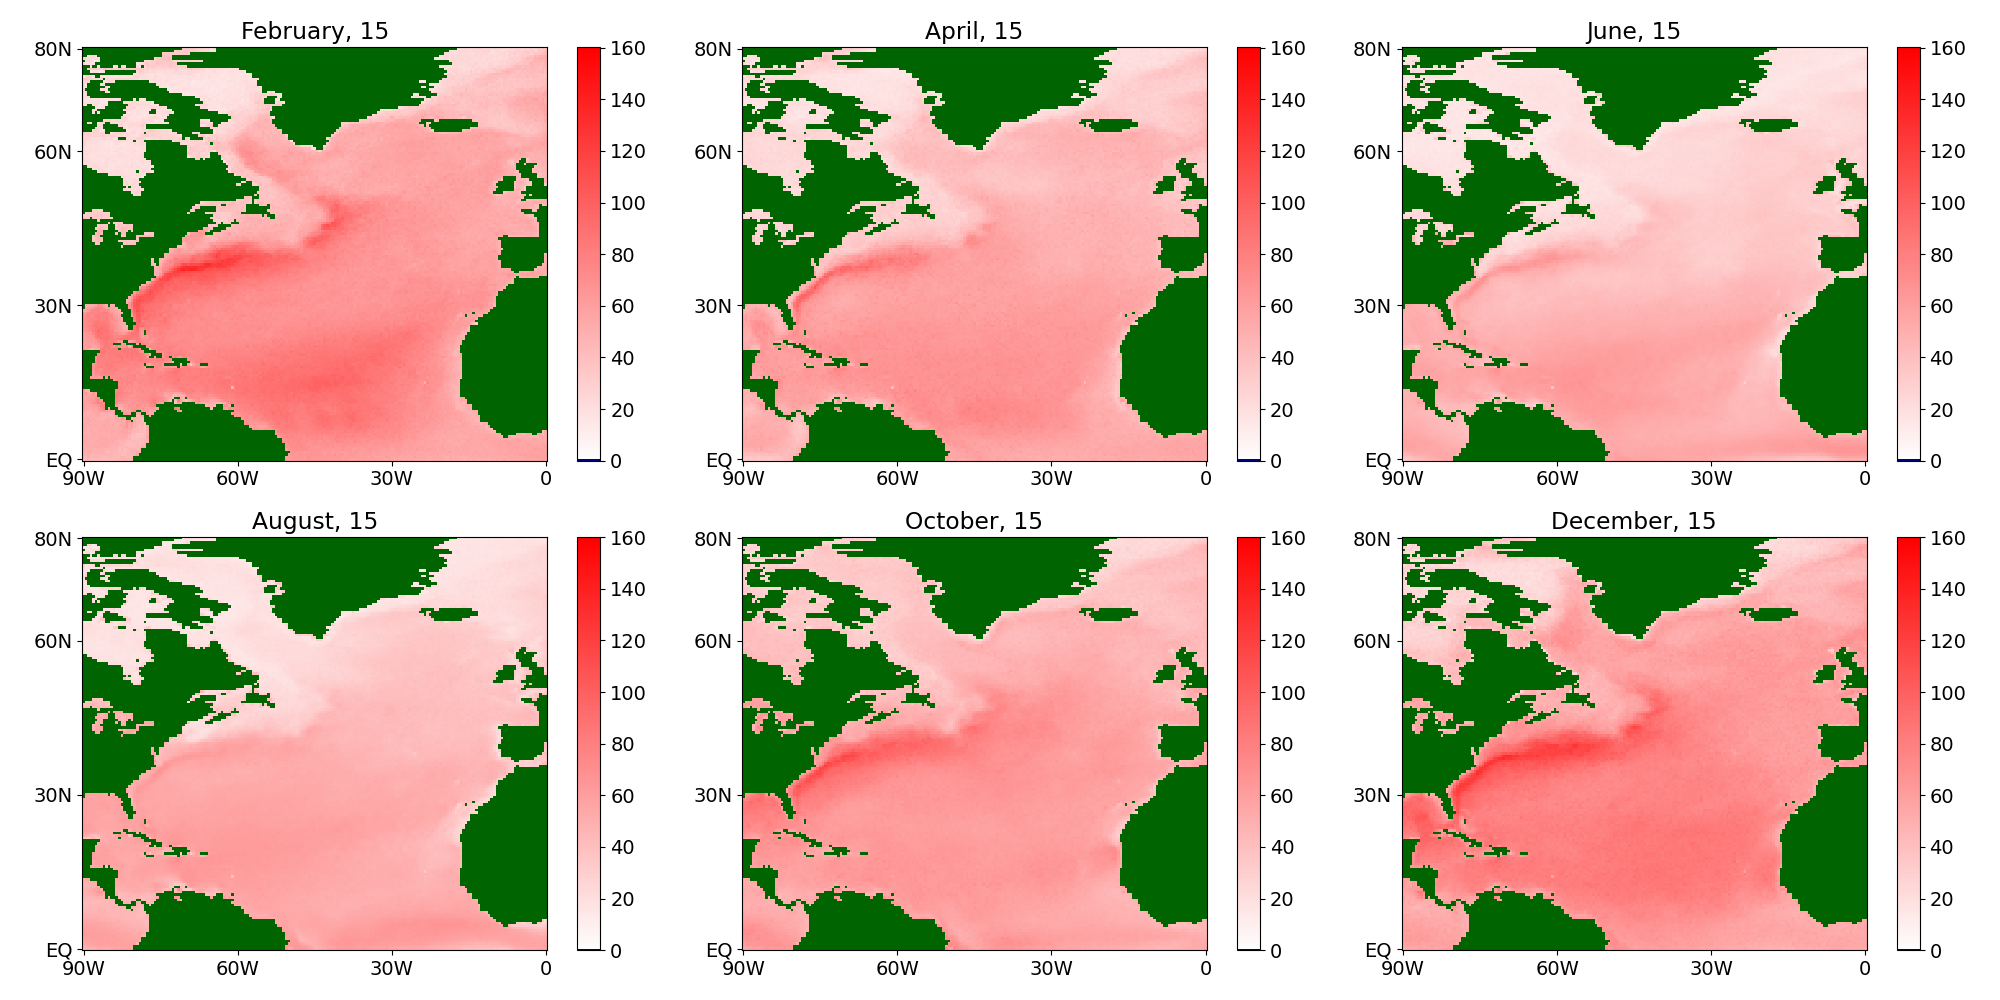
\includegraphics[width=\textwidth]{B22_mean_year}}
	\\
	b)
	
	\caption{Оценки коэффициента $b_{11}(t,X)$ для явного потока (a) и коэффициента $b_{22}(t,X)$ для скрытого потока (b) в течение среднего года}
	\label{fig_b_mean_year}
\end{figure} 

По результатам анализа многолетних данных установлено, что для коэффициента $b(t,X)$ явно прослеживается обратная зависимость для элементов $b_{12}(t,X)$ и $b_{21}(t,X)$: на картах более светлые области для одного являются более яркими для второго, и наоборот. Для оценок $b_{11}(t,X)$ и $b_{22}(t,X)$ характерны те же сезонные свойства, что и для коэффициента сноса $a(t,X)$: в зимние периоды абсолютные значения границ диапазона между квантилями порядка $0.1$ и $0.9$ больше, чем в летние месяцы (см. табл.~\ref{table_quantiles_b}). Наиболее высокие значения диффузионной составляющей встречаются в центральных и южных районах Cеверной Атлантики. 

\begin{table}[h!]
	\centering
	\caption{Диапазоны значений в летний и зимний периоды между квантилями уровня $0.1$ и $0.9$ для $b_{11}$ и $b_{22}$}
	\begin{tabular}{|c|c|c|c|c|}
		\hline
		Период & 1979-1989гг. &  1989-1999гг. & 1999-2009гг. & 2009-2019гг.\\
		\hline
		$b_{11}$, лето & $[10.5, 59.1]$ & $[10.5, 58.5]$ & $[10.8, 60.7]$ & $[10.8, 61.4]$\\ 
		\hline
		$b_{11}$, зима & $[18.5, 76.0]$ & $[18.8, 78.3]$ & $[19.8, 81.9]$ & $[18.5, 78.5]$\\ 
		\hline
		$b_{22}$, лето & $[14.1, 63.5]$ & $[14.0, 63.9]$ & $[14.9, 66.2]$ & $[14.8, 66.8]$\\ 
		\hline
		$b_{22}$, зима & $[22.6, 86.0]$ & $[22.4, 88.6]$ & $[24.3, 90.3]$ & $[22.4, 91.1]$\\ 
		\hline
	\end{tabular}
	\label{table_quantiles_b}
\end{table}


Матрица диффузии показывает области, где преобладает непосредственное взаимодействие океана с атмосферой (при небольших значениях коэффицента сноса). Отметим, что обратная соотношение между данными величинами, то есть небольшая диффузия и значительный коэффициент сноса,  характеризует перенос потока тепла не только в атмосферу, но и внутри океана.

В зимние месяцы выделяется <<красная>> зона вдоль основного течения Гольфстрима и к северу от $40^\circ$~с.ш. (см. рис.~\ref{fig_b_mean_year}b), %также \degree из gensymb
где сильны взаимодействия как явного так и скрытого потоков за счет разности тепла и влаги между океаном и атмосферой. Также надо отметить роль сильных ветров в зимние месяцы (шторм-треки циклонов), которые в значительной степени формируют этот обмен. С учетом того, что квадрат коэффициента диффузии дает оценки энергобаланса между океаном и атмосферой, на приведенных картах можно выделить области с наибольшей энергоактивностью, прежде всего, для графиков зависимости между скрытым и явным потоками. В качестве энергоактивных областей, по классификации Г.И.Марчука~\cite{marchuk1989}, можно выделить Ньюфаундленский и Норвежский полигоны. 

\section{Взаимосвязь динамической и диффузионной составляющих процесса}
В данном разделе рассматривается взаимосвязь коэффициентов сноса и диффузии СДУ Ито~\eqref{Ito} для явных и скрытых потоков тепла. 

Сначала рассмотрим поведение выборочного коэффициента корреляции Пирсона: для двух выборок $x = (x_1, \dots, x_m)$ и $y = (y_1, \dots, y_m)$ размерности $m$ он определяется следующим образом
\begin{equation}
	\label{Pearson}
	r_{xy} = \frac{\sum_{i=1}^{m}(x_i - \overline{x})(y_i - \overline{y}) }{\sqrt{\sum_{i=1}^{m}(x_i - \overline{x})^2 \sum_{i=1}^{m}(y_i - \overline{y})^2}}.
\end{equation}

Рассматривается поведение оценок $(a_1, a_2)$ и $(b_{11}, b_{22})$
в режиме скользящего окна ширины $14$ дней, то есть в качестве векторов $x$ и $y$ из \eqref{Pearson} выступают наборы $(a_1(t), a_1(t+1), \dots, a_1(t+14)), (a_2(t), a_2(t+1), \dots, a_2(t+14))$ и $(b_{11}(t), b_{11}(t+1), \dots, b_{11}(t+14)), (b_{22}(t), b_{22}(t+1), \dots, b_{22}(t+14))$, а размерность векторов $m=14$.

\begin{figure}[!h]
	\centering
	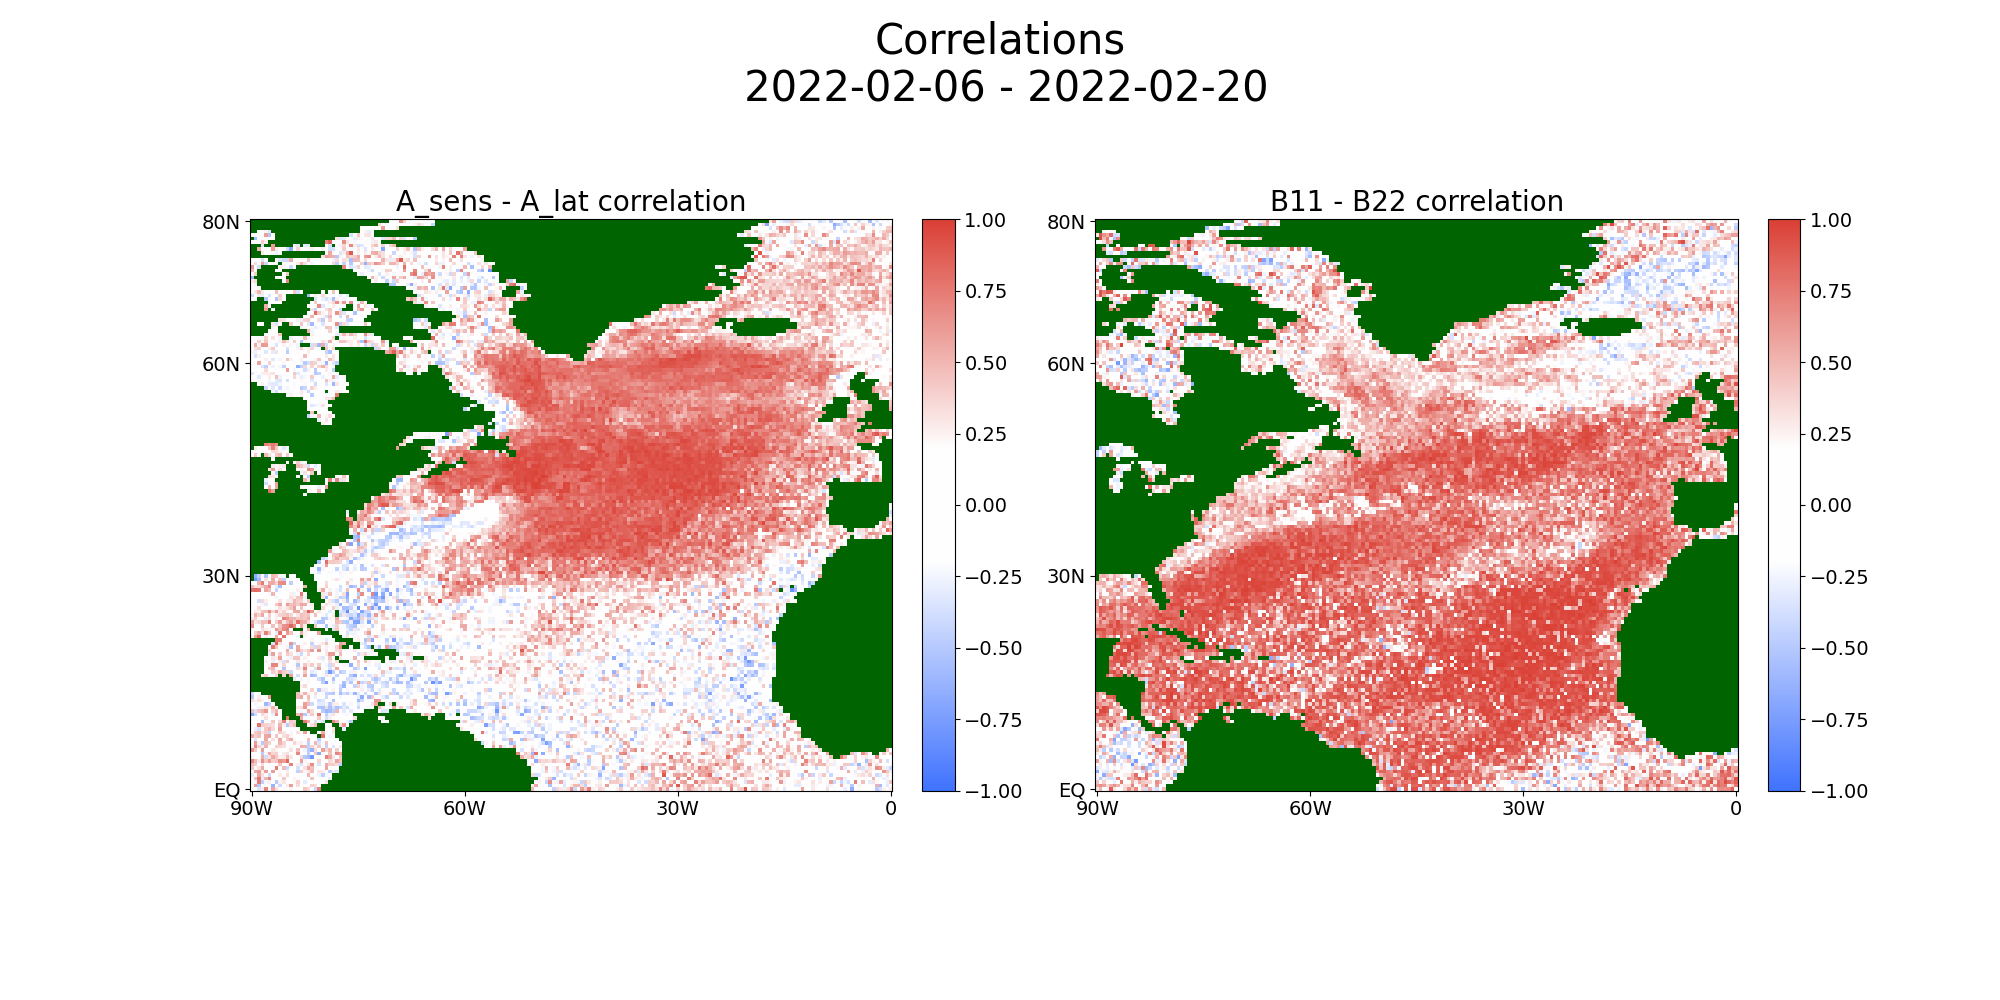
\includegraphics[width=\textwidth]{C_15742}
	\caption{Пример корреляций между оценками коэффициентов сноса (карта слева) и диффузии (карта справа)}
	\label{fig_c_example}
\end{figure}

На рисунке~\ref{fig_c_example} показан пример полученной корреляции для коэффициентов сноса (карта слева) и диффузии (карта справа) явных и скрытых потоков. Цветовая шкала меняется от синего при отрицательных значениях до до красного при положительных, белый цвет соответствует оценкам, близким к $0$. Яркость цвета в конкретной точке соответствует удаленности значения от нуля. Минимум и максимум шкалы естественным образом равны $-1$ и $1$, соответственно. Темно-зеленым цветом, как и ранее, обозначена суша. Для коэффициента сноса в области Саргассова моря периодически наблюдаются области с отрицательной корреляцией, для диффузиозной составляющей же это обыкновенно области Норвежского моря, Гудзонова залива и моря Баффина. В зимние месяцы корреляция двух компонент коэффициента сноса существенно положительна в широком коридоре вдоль течения Гольфстрима, а в летние месяцы коридор положительных значений существенно сужается. Отрицательные значения встречаются редко и визуально равномерно распределены по всей карте, и встречаются как в летние, так и в зимние периоды.

\begin{figure}[h!]
	\centering
	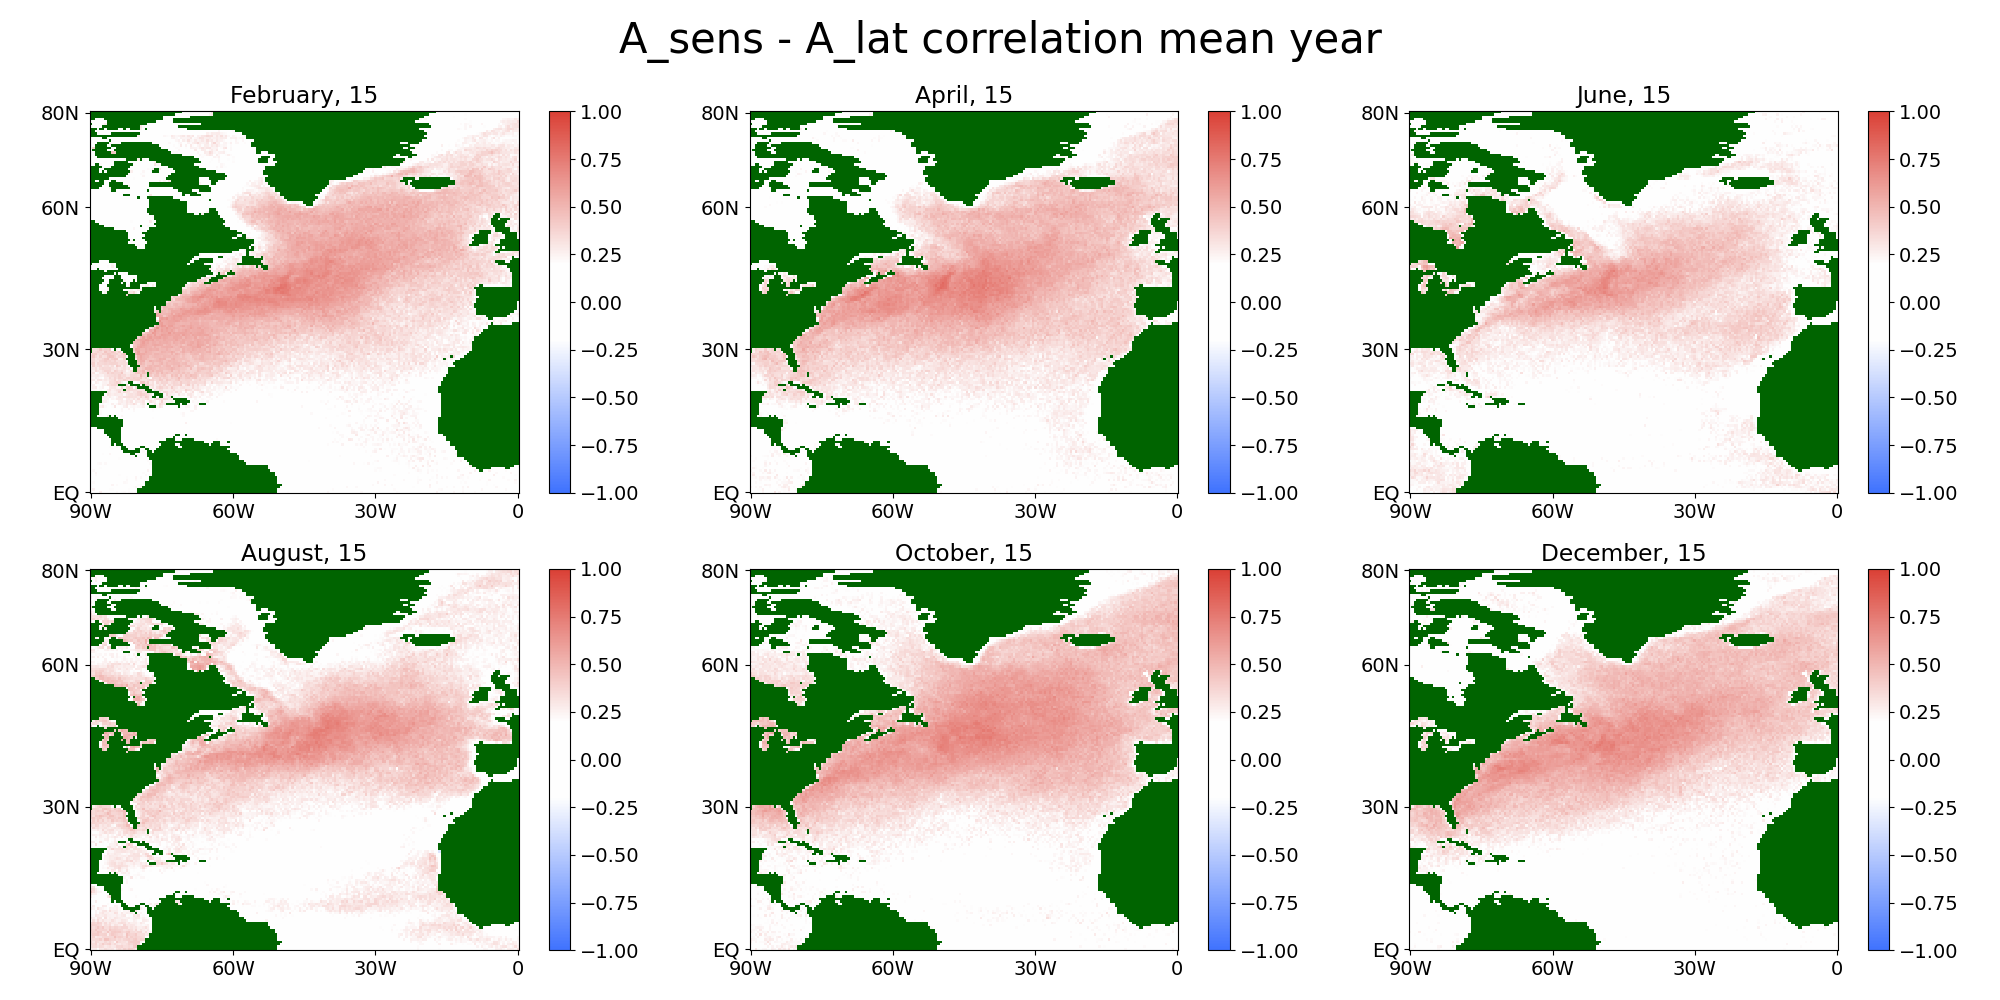
\includegraphics[width=\textwidth]{C_0_mean_year}
	\caption{Корреляции между $a_1$ и $a_2$ в течение среднего года}
	\label{fig_c0}
\end{figure}

\begin{figure}[h!]
	\centering
	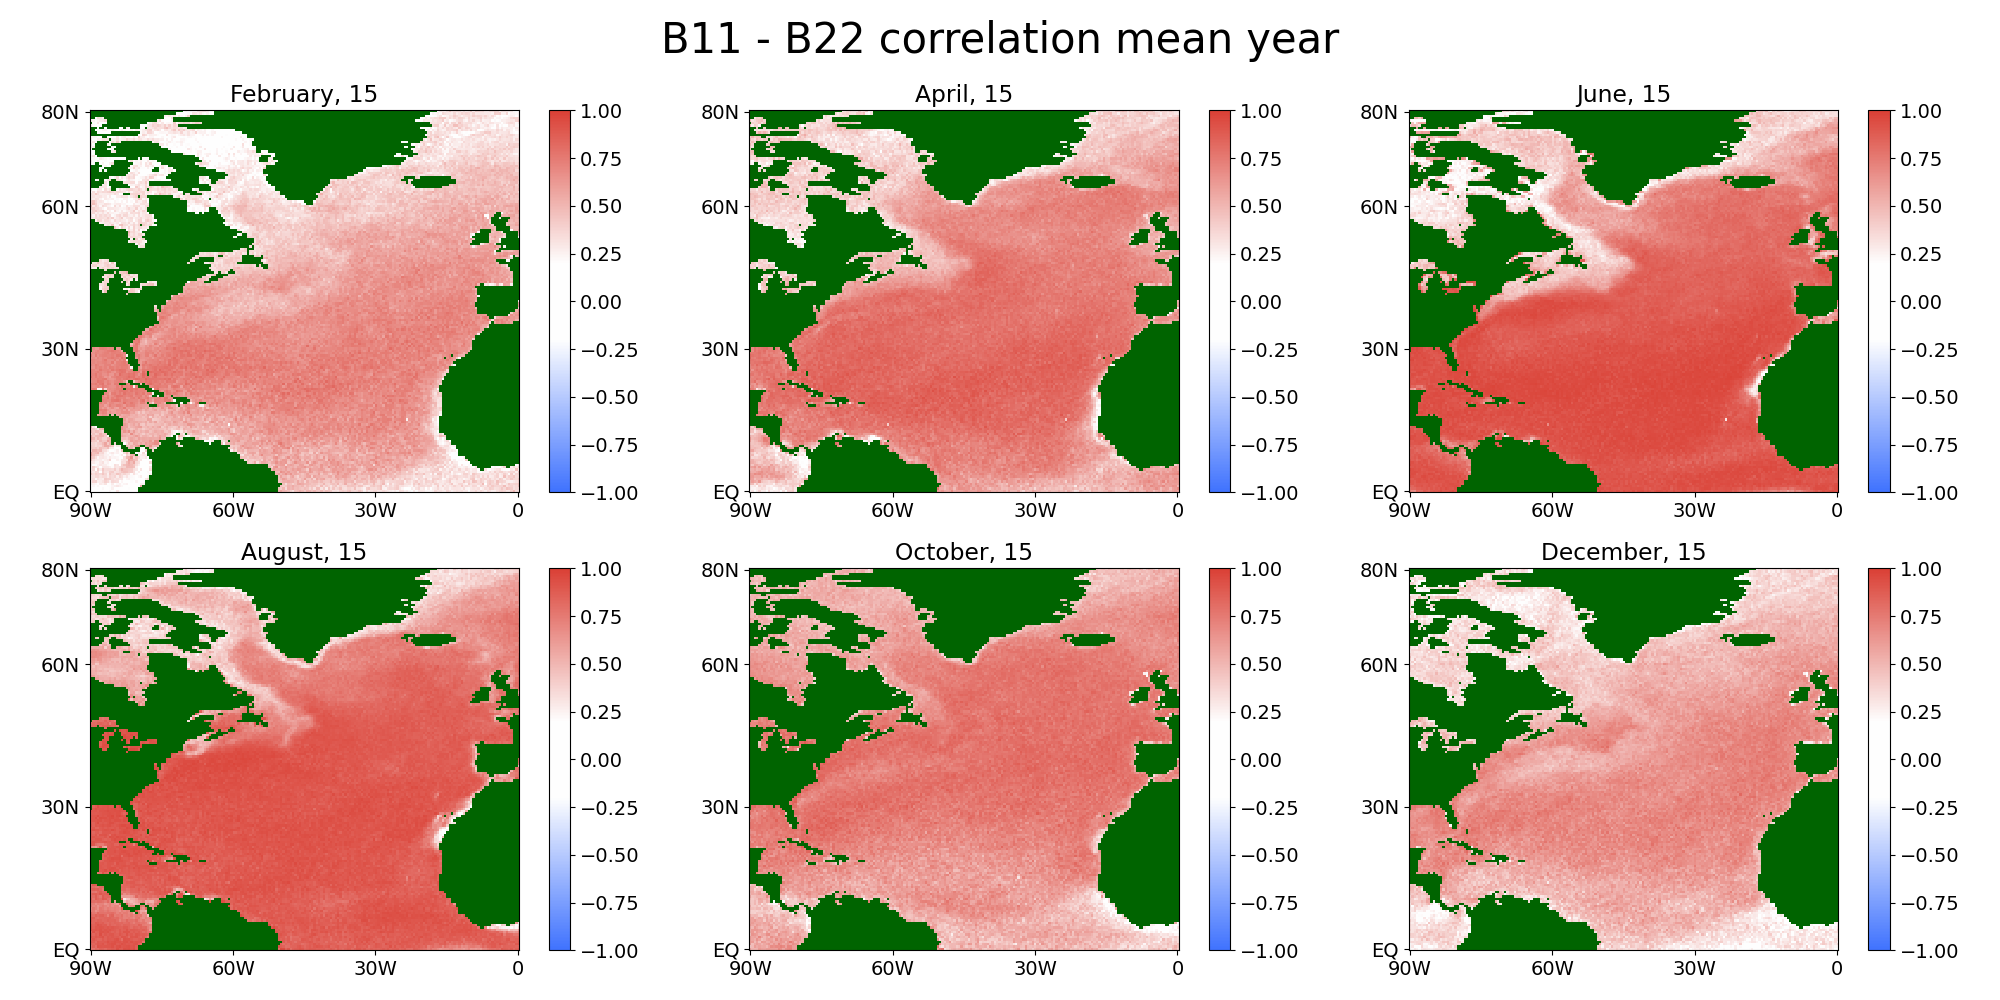
\includegraphics[width=\textwidth]{C_1_mean_year}
	\caption{Корреляции между $b_{11}$ и $b_{22}$ в течение среднего года}
	\label{fig_c1}
\end{figure}

На рисунках~\ref{fig_c0} -~\ref{fig_c1} показаны корреляции между парами $(a_1, a_2)$ и $(b_{11}, b_{22})$ в течение среднего года. Видно, что коэффициенты диффузии имеют значительно более высокий процент положительной корреллированности, при этом значения близки к $1$. Для коэффициентов сноса такая область в акватории примерно в два раза меньше по площади, значения корреляции значительно меньше. 

Очевидно, что коэффициенты сноса и диффузии оцениваются не точно. Стого получить доверительные интервалы этих оценок без дополнительных достаточно неочевидных предположений невозможно. Однако полученные коэффициенты корреляции показывают, насколько сильно эти коэффициенты связаны, возможно ли по одному из них восстановить или оценить другой. Из приведенных катринок видно, что коэффициенты диффузии в тех районах, где они близки к $1$, определены достаточно адекватно. Для коэффициентов сноса достаточно хорошо выделяются районы стуйных течений. В то же время, в южной и центральной частях Северной Атлантики течения слабо заметны, и поэтому корреляция мала.

% 	\subsection{Анализ вклада динамической и диффузиозной составляющих}
Теперь рассмотрим величину $F$, отражающую соотношение между коэффициентами $a(t,X)$ и $b(t,X)$, для каждой точки сетки с координатами $(x,y)$ в момент времени $t \in [0,T]$: 
\begin{equation}
	F(x,y,t) = \frac{|a_1(x,y,t) + a_2(x,y,t)|}{\sqrt{b_{11}^2(x,y,t) + b_{22}^2(x,y,t) + b_{12}(x,y,t) + b_{21}(x,y,t)}}.
\end{equation}

Физический смысл данной величины связан с оценкой энергии потоков как внутри океана, так и при отдаче тепла в или из атмосферы. 
% 	На рисунке~\ref{fig_f_example} показан пример визуализации данной характеристики. \textcolor{yellow}{Не заменить ли его на  а-ля средний год?} 
На рисунке~\ref{fig_f_mean_year} представлено поведение рассматриваемой величины в течение среднего года.
% 	Цветовая шкала в данном случае является дискретной, в ней присутствуют $5$ цветов. Глубина цвета в каждой области одинаковая и не зависит от удаленности значения от границ соответствующего отрезка.

% 	\begin{figure}[h!]
	% 		\center{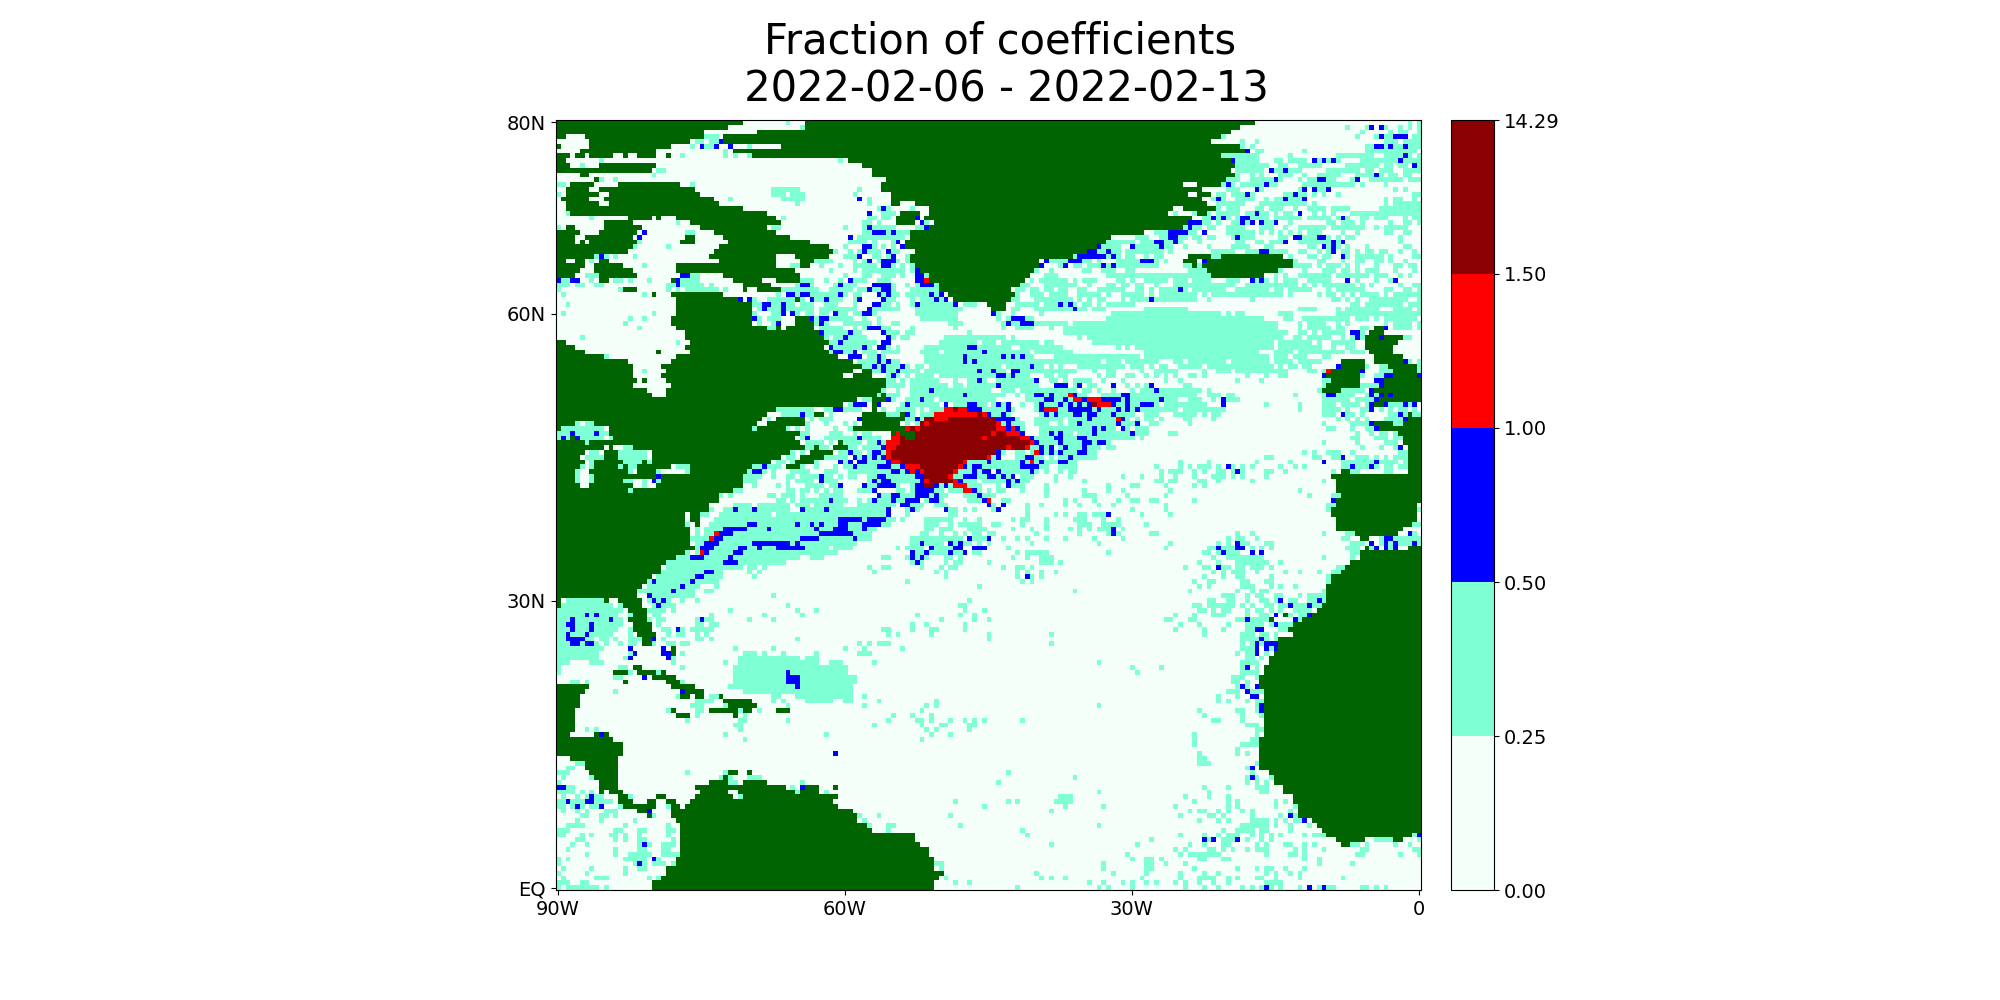
\includegraphics[width=\textwidth]{FN_15742}}
	% 		\caption{Преобладание диффузионной компоненты процесса в акватории Северной Атлантики, февраль 2022 года}
	% 		\label{fig_f_example}
	% 	\end{figure}

\begin{figure}[!h]
	\centering
	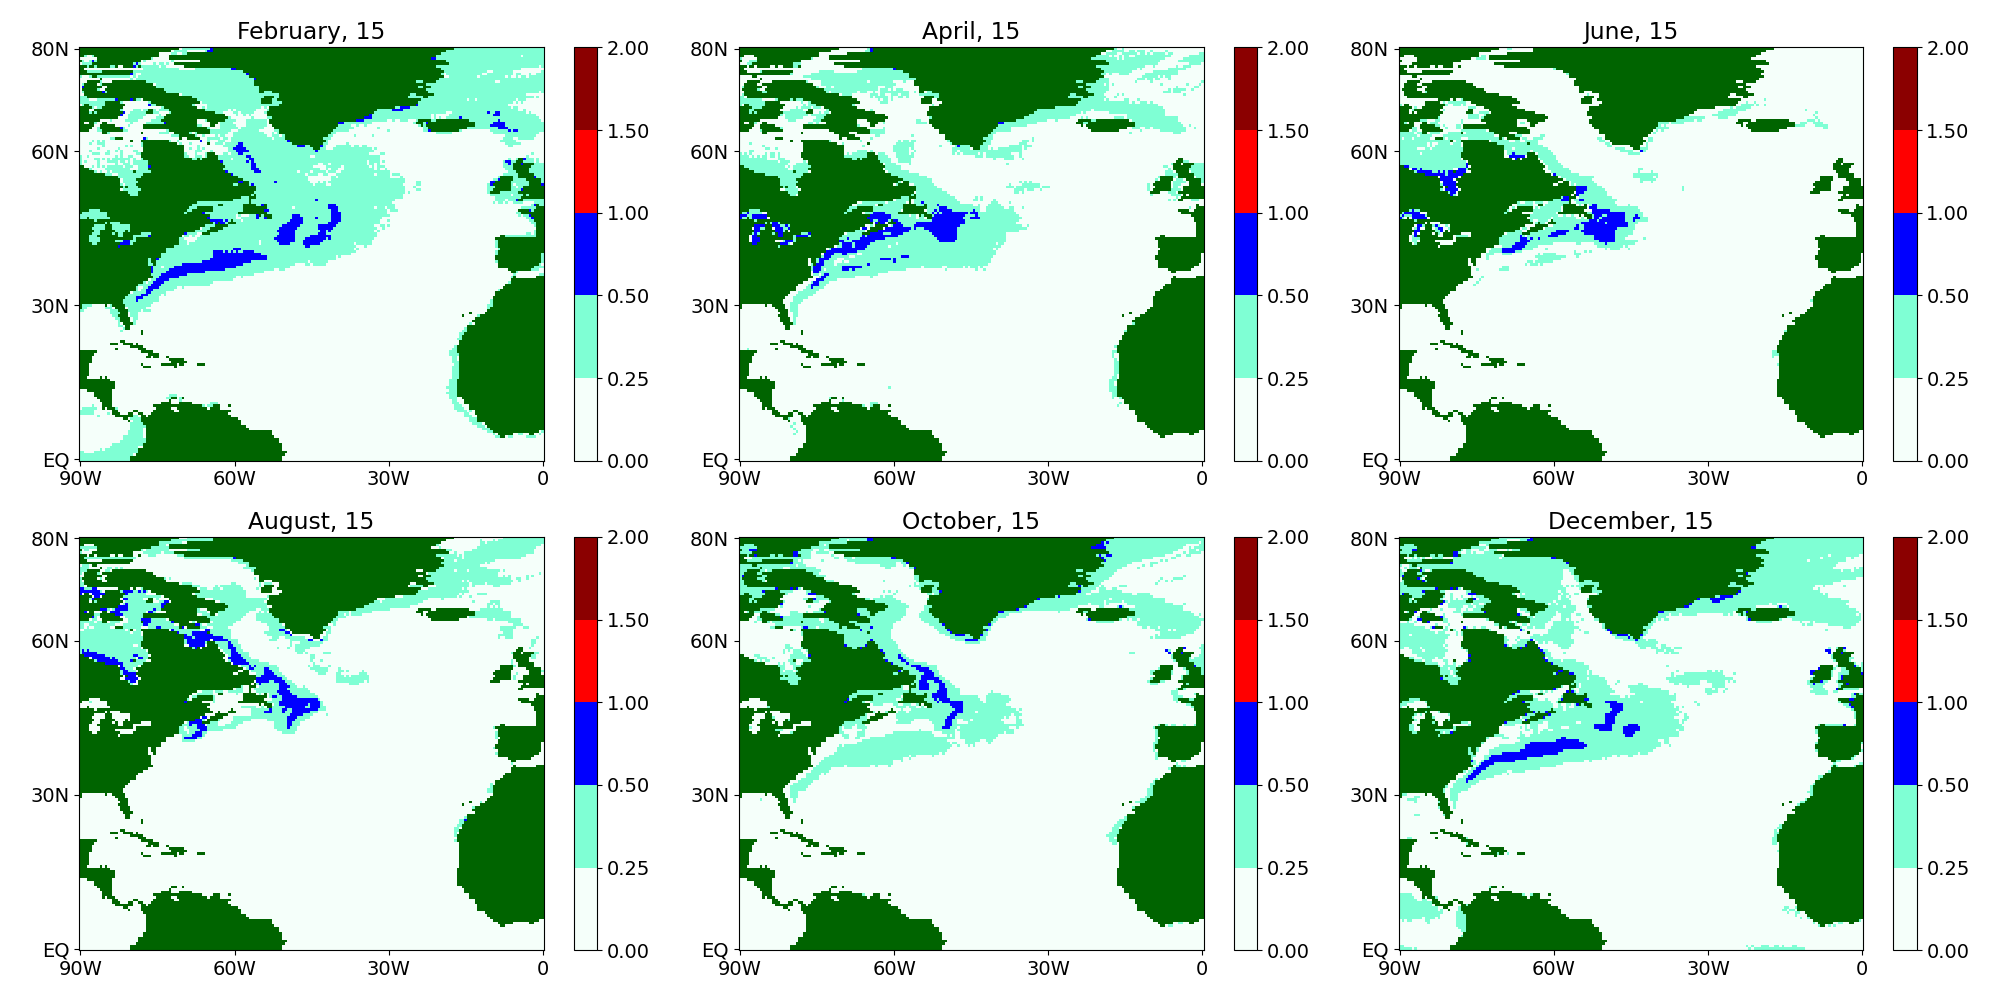
\includegraphics[width=\textwidth]{F_mean_year}
	\caption{Преобладание диффузионной компоненты процесса в акватории Северной Атлантики в течение среднего года}
	\label{fig_f_mean_year}
\end{figure}

Цветовая шкала в данном случае является дискретной, в ней присутствуют $5$ цветов. Интенсивность цвета в каждой области одинаковая и не зависит от удаленности значения от границ соответствующего отрезка. Набольшие значения величины $F$ возникают, в основном, вдоль течения Гольфстрима, а также, как и ранее, средние значения по всей акватории больше в зимний период, чем в летний. При этом в большей части акватории Северной Атлантики за весь анализируемый период преобладают значения величины $F$, не превышающие $0.5$, что говорит о преобладании диффузионной составляющей процесса. Квадрат диффузии показывает количественно вклад отдельных регионов в энергообмен океан--атмосфера, поэтому даные результаты важны с точки зрения оценок энергобаланса.

\section{Поведение характеристик коэффициентов}

В данном разделе рассмотрено поведение таких характерных величин полученных оценок, как максимум, минимум и среднее, вычисляемых по всей акватории.
Им соответствуют красный, синий и зеленый цвета на графиках далее.
% 	Отметим, что также рассматривалось поведение медианы, но оно полностью аналогично среднему, поэтому в дальнейшем не упоминается.

Сначала рассмотрим изменение этих характеристик в рамках одного года. Для примера на рисунке~\ref{fig_ab_daily} приведены данные для коэффициентов сноса и диффузии за $2021$ год для явных и скрытых потоков (верхний и нижний графики).
Среднее почти постоянно и испытывает лишь небольшие отклонения от нуля, максимумы и минимумы же обладают ярко выраженной сезонностью. Как уже отмечалось ранее, в летний период (примерно с мая по октябрь) значения оценок $a(t,X)$ и $b(t,X)$ по модулю заметно меньше, чем в остальное время года. 

\begin{figure}[!h]
	\centering
	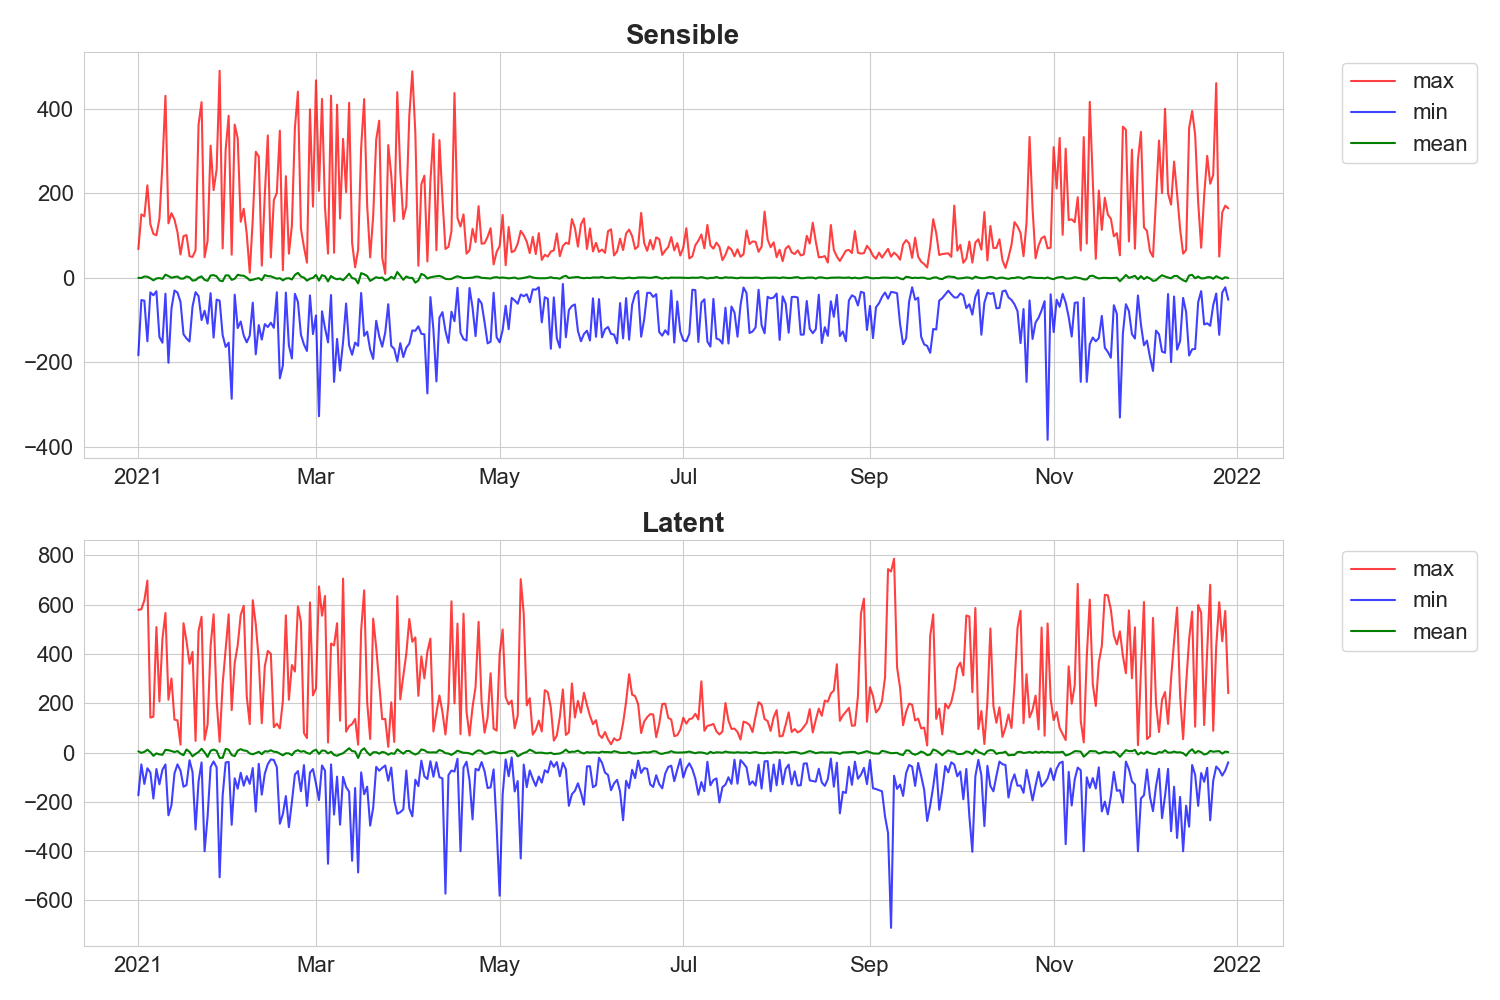
\includegraphics[width=\textwidth]{a_(15341-15705)_1}\\
	a)
	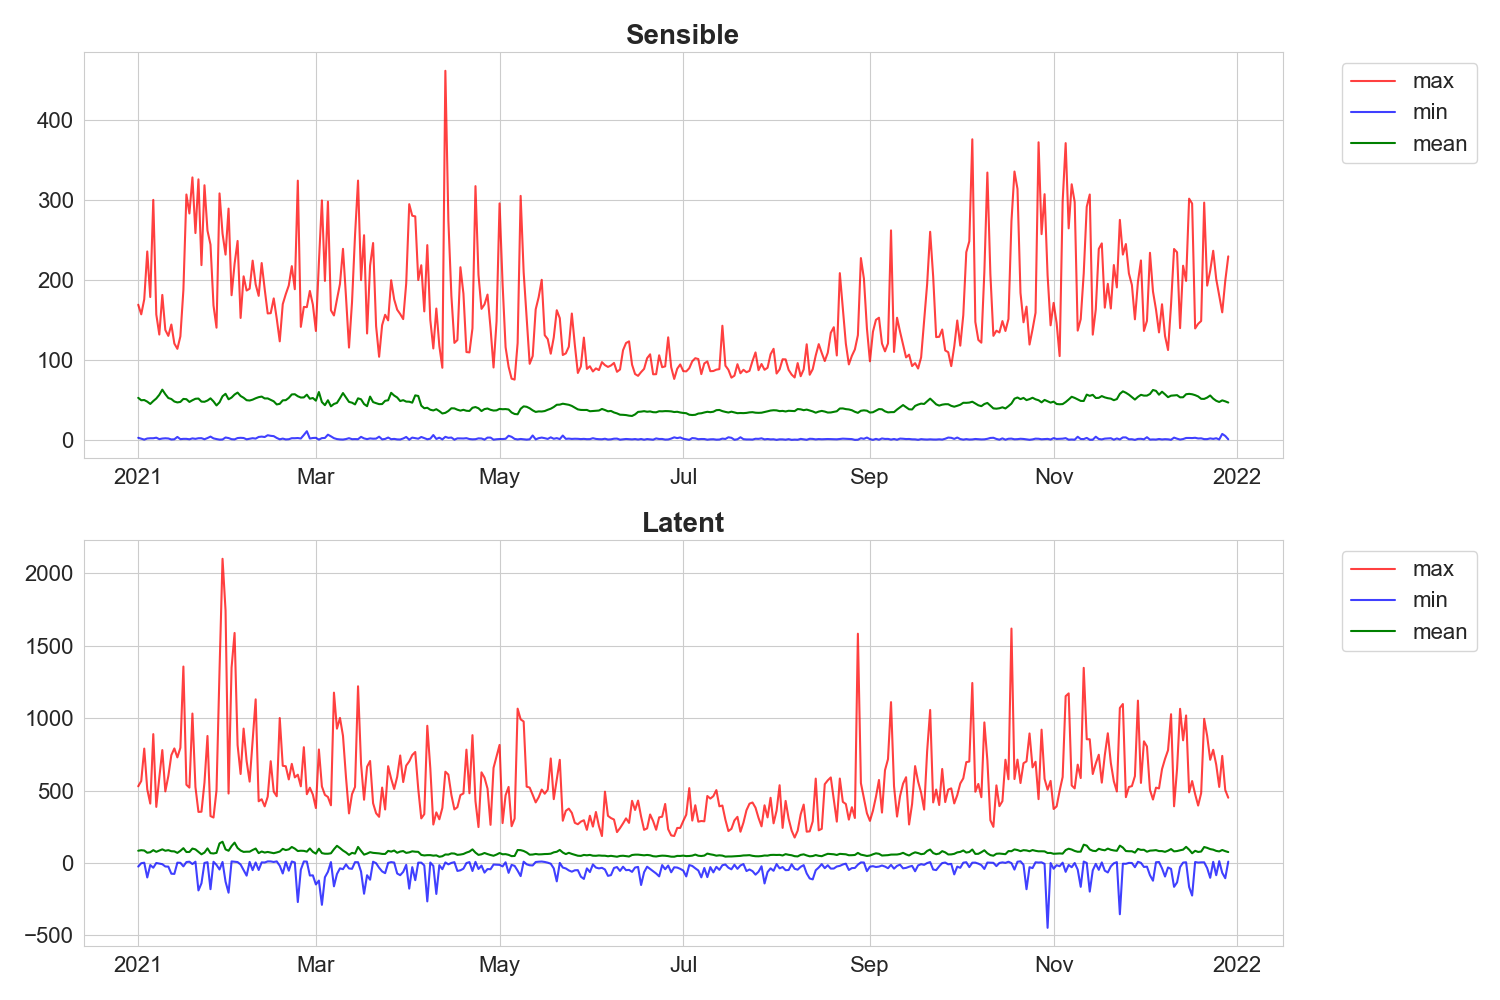
\includegraphics[width=\textwidth]{b_(15341-15705)_1}
	\\
	b)
	
	\caption{Поведение характеристик оценок коэффициентов сноса (а) и диффузии (b) для явных и скрытых потоков в течение $2021$ года с шагом в $1$ день}
	\label{fig_ab_daily}
\end{figure}

\begin{figure}[h!]
	\centering
	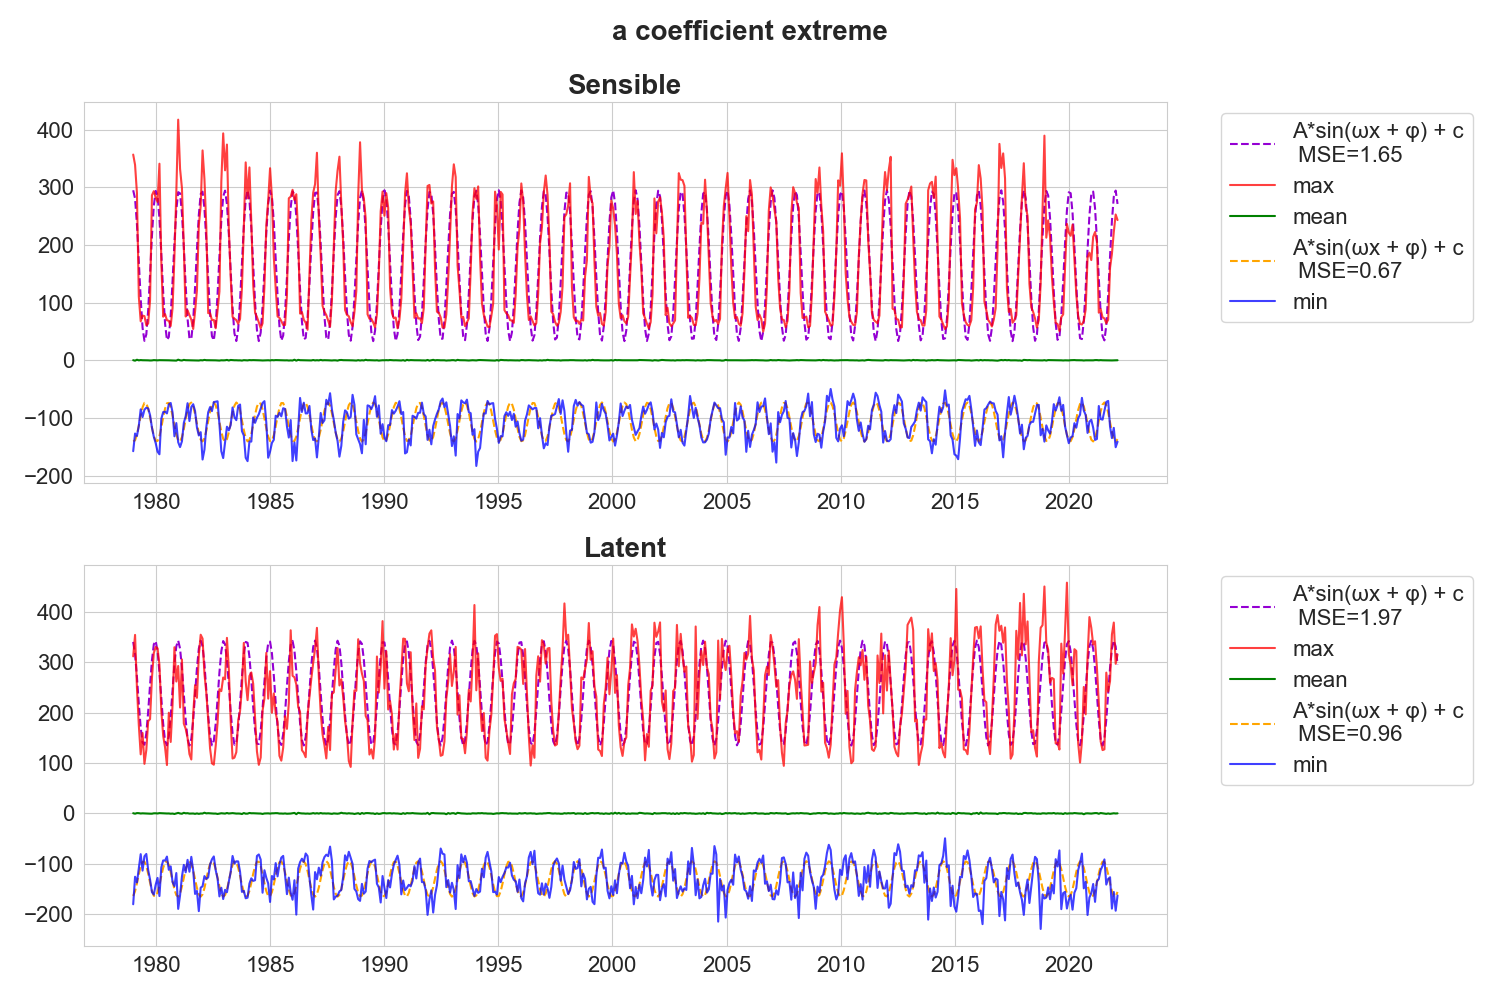
\includegraphics[width=\textwidth]{a_(1-15797)_30_fit}\\
	a)
	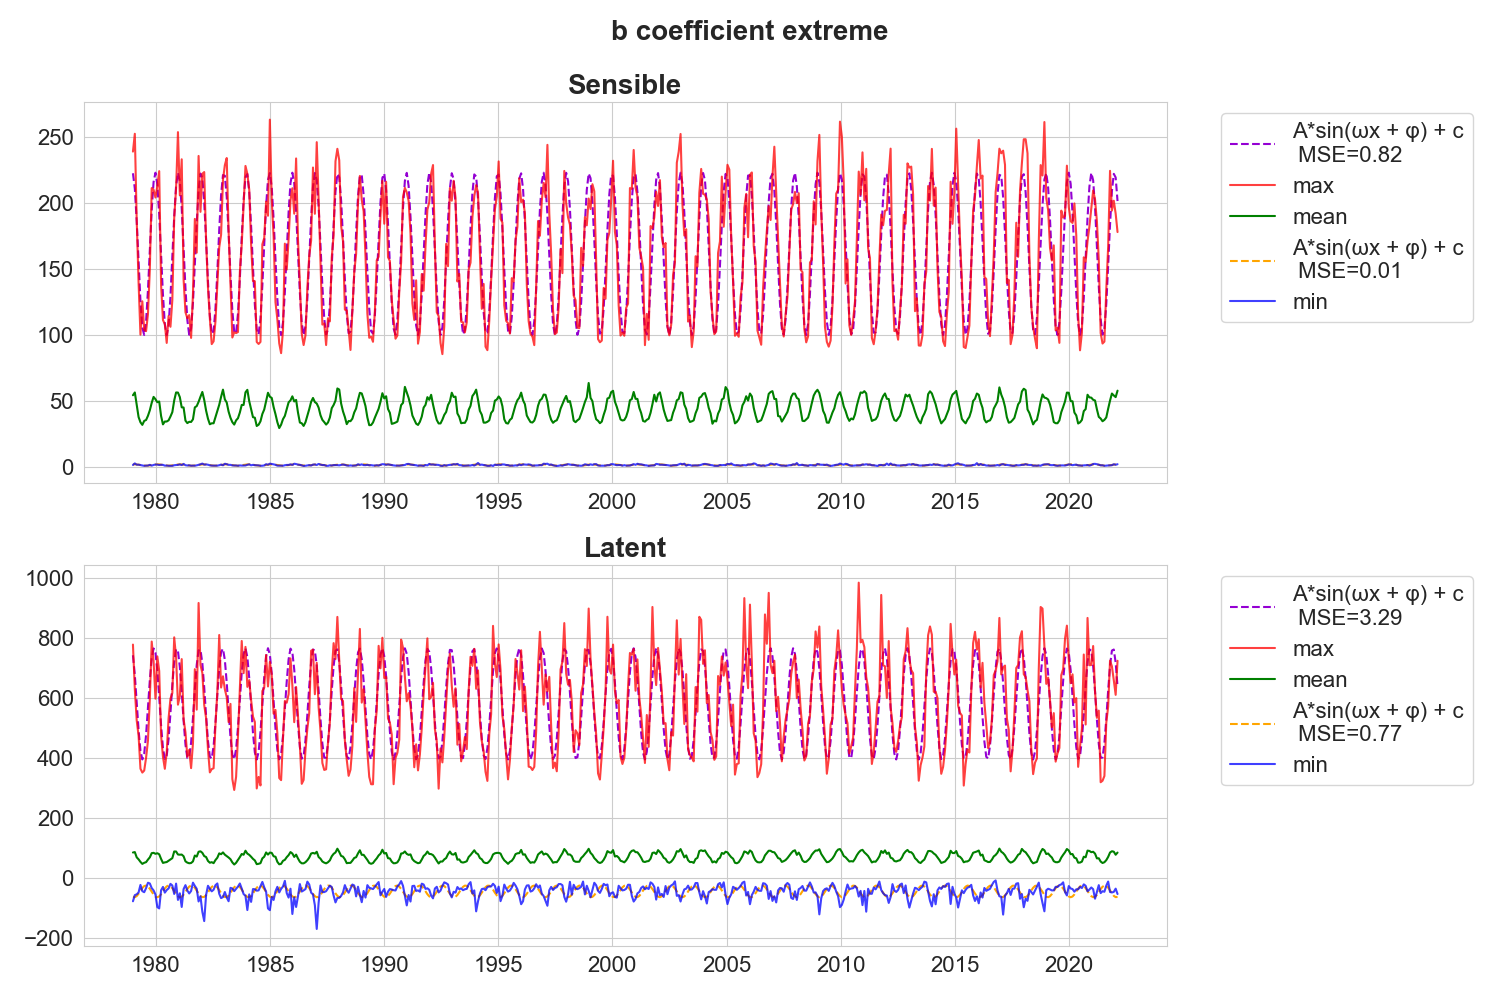
\includegraphics[width=\textwidth]{b_(1-15797)_30_fit}\\
	b)
	\caption{Поведение экстремальных характеристик оценок коэффициентов сноса (a) и диффузии (b) $1979$--$2021$~гг. с шагом в $30$ дней}
	\label{fig_ab_monthly}
\end{figure}

При рассмотрении усреднений в $30$ и $365$ дней наблюдается ярко выраженная сезонность в поведении максимумов и минимумов. Поэтому для них построена аппроксимация соответствующих кривых с помощью синусоидальной функции вида $A \cos{\omega x + \phi} + c$. На рисунке~\ref{fig_ab_monthly} представлено изменение рассматриваемых характеристик в течение $1979$--$2021$~гг., усредненных по последовательным отрезкам времени длиной $30$ дней, а также найденные функции вместе с соответствующей среднеквадратичной ошибкой приближения. С точки зрения геофизики, эти величины показывают регулярность рассматриваемого ряда в его средне- и долгосрочной изменчивости.

\begin{figure}[h!]
	\centering
	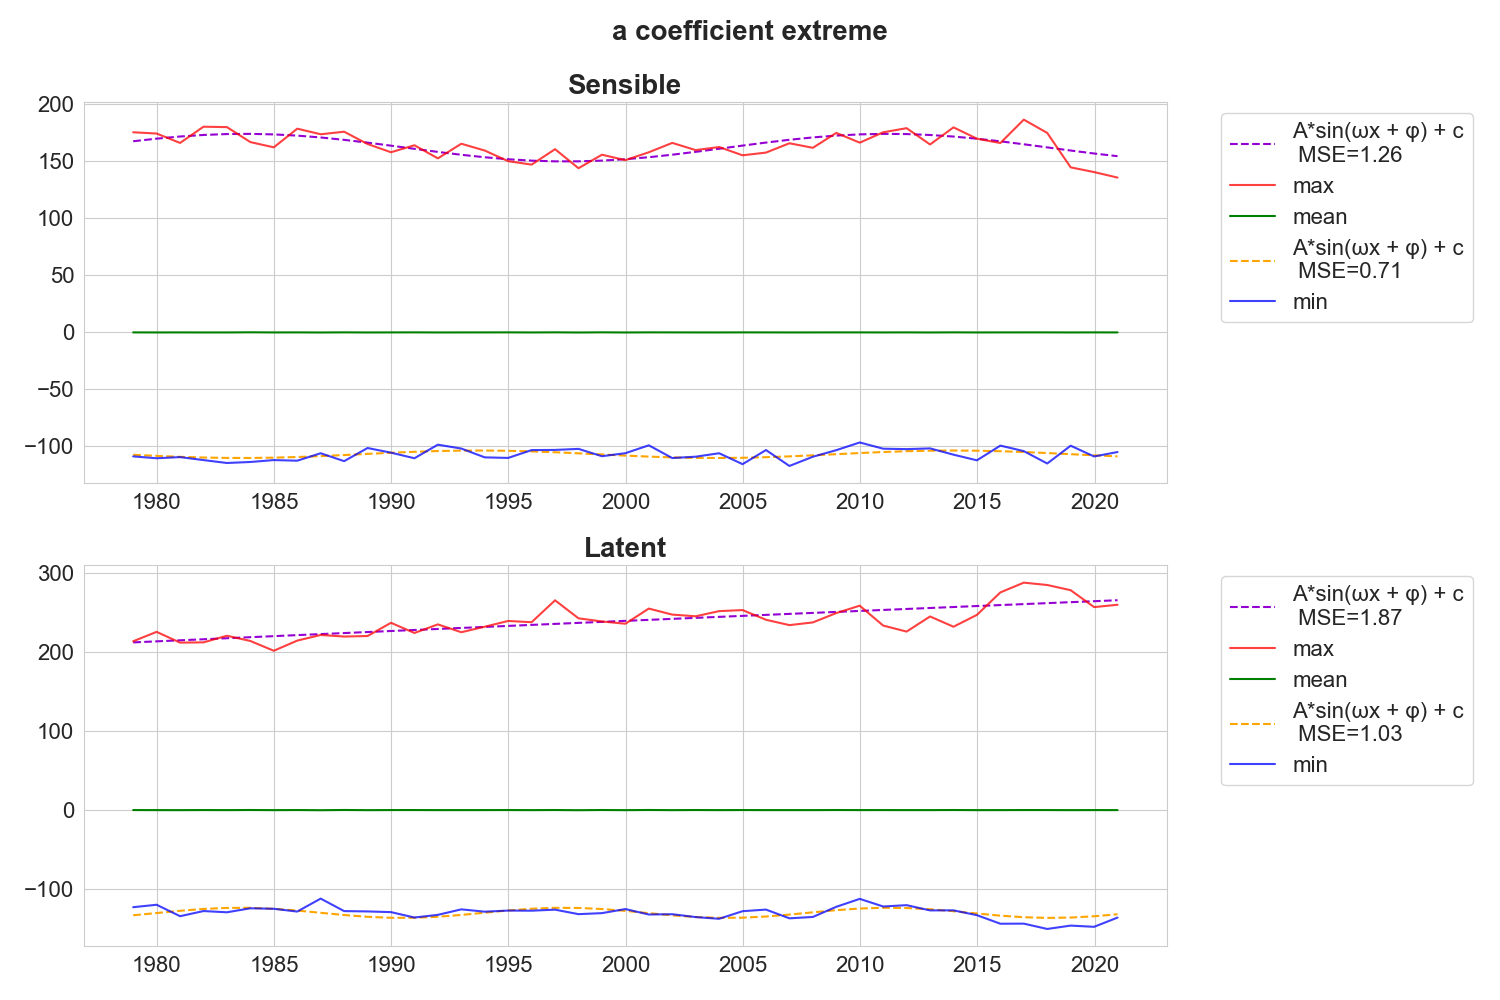
\includegraphics[width=\textwidth]{a_(1-15797)_365_fit}\\
	a)
	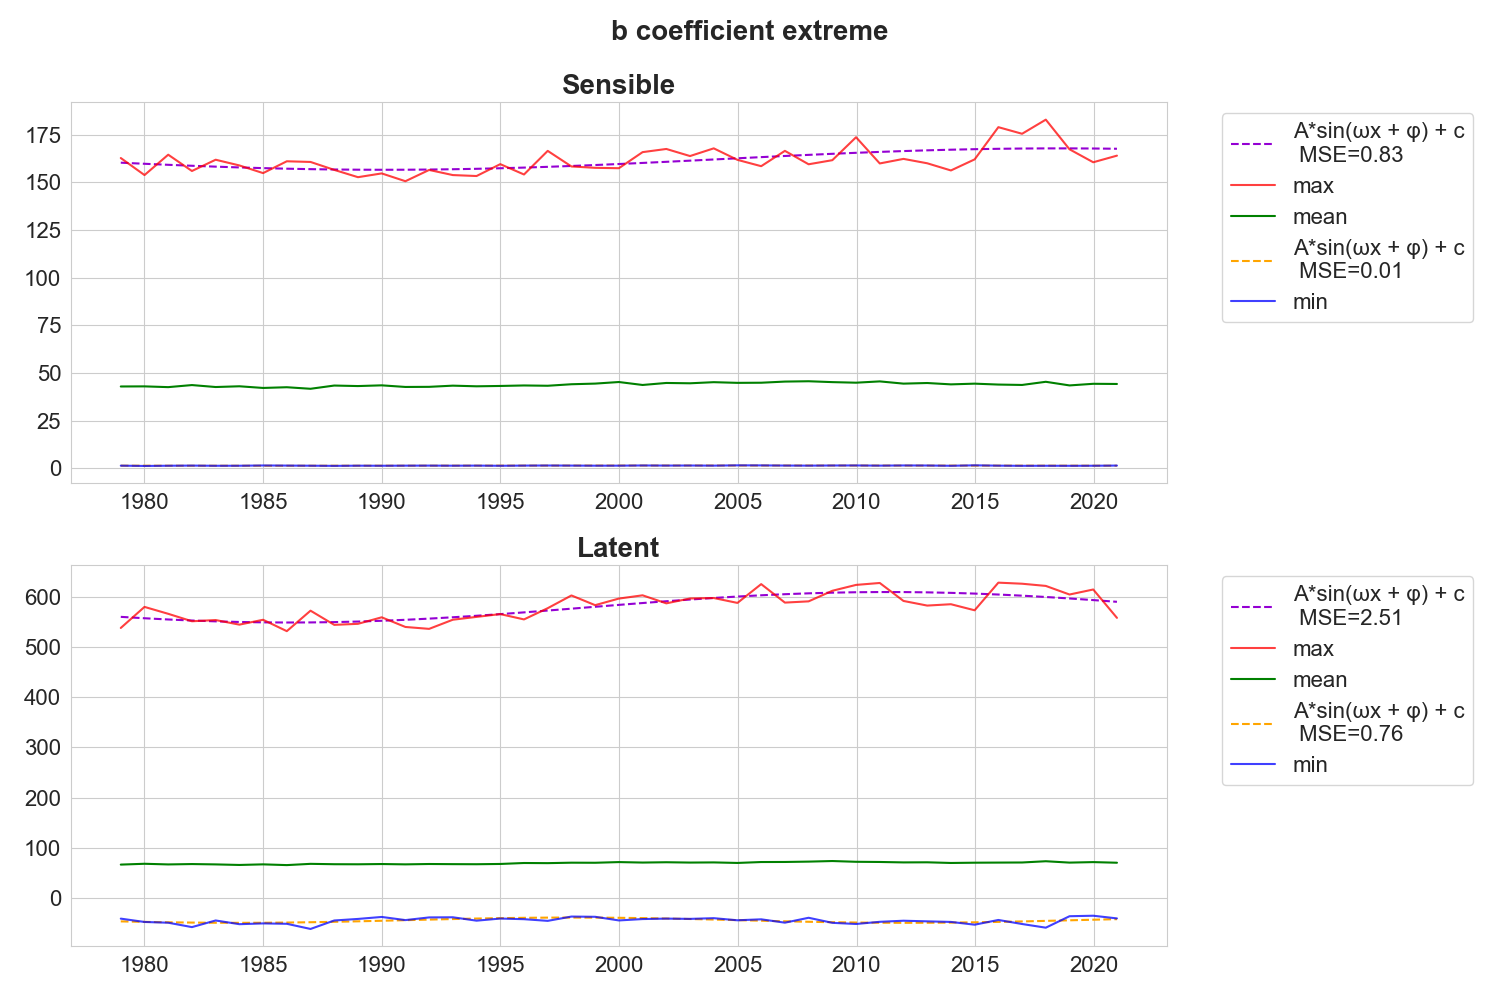
\includegraphics[width=\textwidth]{b_(1-15797)_365_fit}\\
	b)
	\caption{Поведение характеристик оценок коэффициентов сноса (a) и диффузии (b) в течение $1979$--$2021$~гг. с шагом в $365$ дней}
	\label{fig_ab_year}
\end{figure}

Рисунок~\ref{fig_ab_year} иллюстрирует изменение рассматриваемых характеристик в течение $1979$--$2021$~гг., усредненных по последовательным отрезкам времени длиной $365$ дней, а также вышеописанные приближения с помощью синусоидальной функции кривых максимума и минимума. На этих графиках сезонность выражена не так ярко. В то же время можно заметить некоторые тренды за промежуток времени длиной в $43$ года. Например, для оценок коэффициента $a(t,X)$, особенно для компоненты $a_2(t,X)$, отвечающей скрытому потоку, видно, что максимум и минимум довольно явно удаляются от линии среднего с течением времени, начиная с $2010$ года. 

\clearpage

\section{Вид зависимости коэффициента сноса от значений потока}
Помимо поведения изучнных выше характеристик коэффициентов, интерес представляет поиск зависимости между ними и коэффициентом сноса $a(t,X)$ для дальнейшего аналитического и численного анализа решения соответсвующего уравнения Ланжевена,  а также для понимания причин формирования характеристик уравнений. Для выявления этих закономерностей покроем весь рассматриваемый период с $1$ января $1979$ г. по $30$ сентября $2022$ года подряд идущими окнами шириной в $30$ и $365$ дней, затем в каждом окне найдем точки, в которых достигались максимум, минимум или среднее потока для обоих типов потоков соответственно, и рассмотрим поведение вычисленных оценок коэффициента $a(t,X)$ в этих точках.

На рисунках~\ref{fig_a_flux_month} и~\ref{fig_a_flux_year} представлена эволюция рассматриваемой зависимости во времени. Здесь красным цветом обозначены значения коэффициента $a$, достигавшиеся в точках максимума потоков, желтым -- в точках медианы, и синим -- в точках минимума потоков. Примечательно, что максимумам потока в оценках коэффициента $a(t,X)$ соответствуют отрицательные значения, а минимумам -- положительные, т.е. наблюдается обратная зависимость. Этот результат вполне ожидаем, так как при значениях максимума и соответственно минимума происходит изменение знака производной потока, то есть происходит переход с роста к убыванию и наоборот.

\begin{figure}[!h]
	\centering
	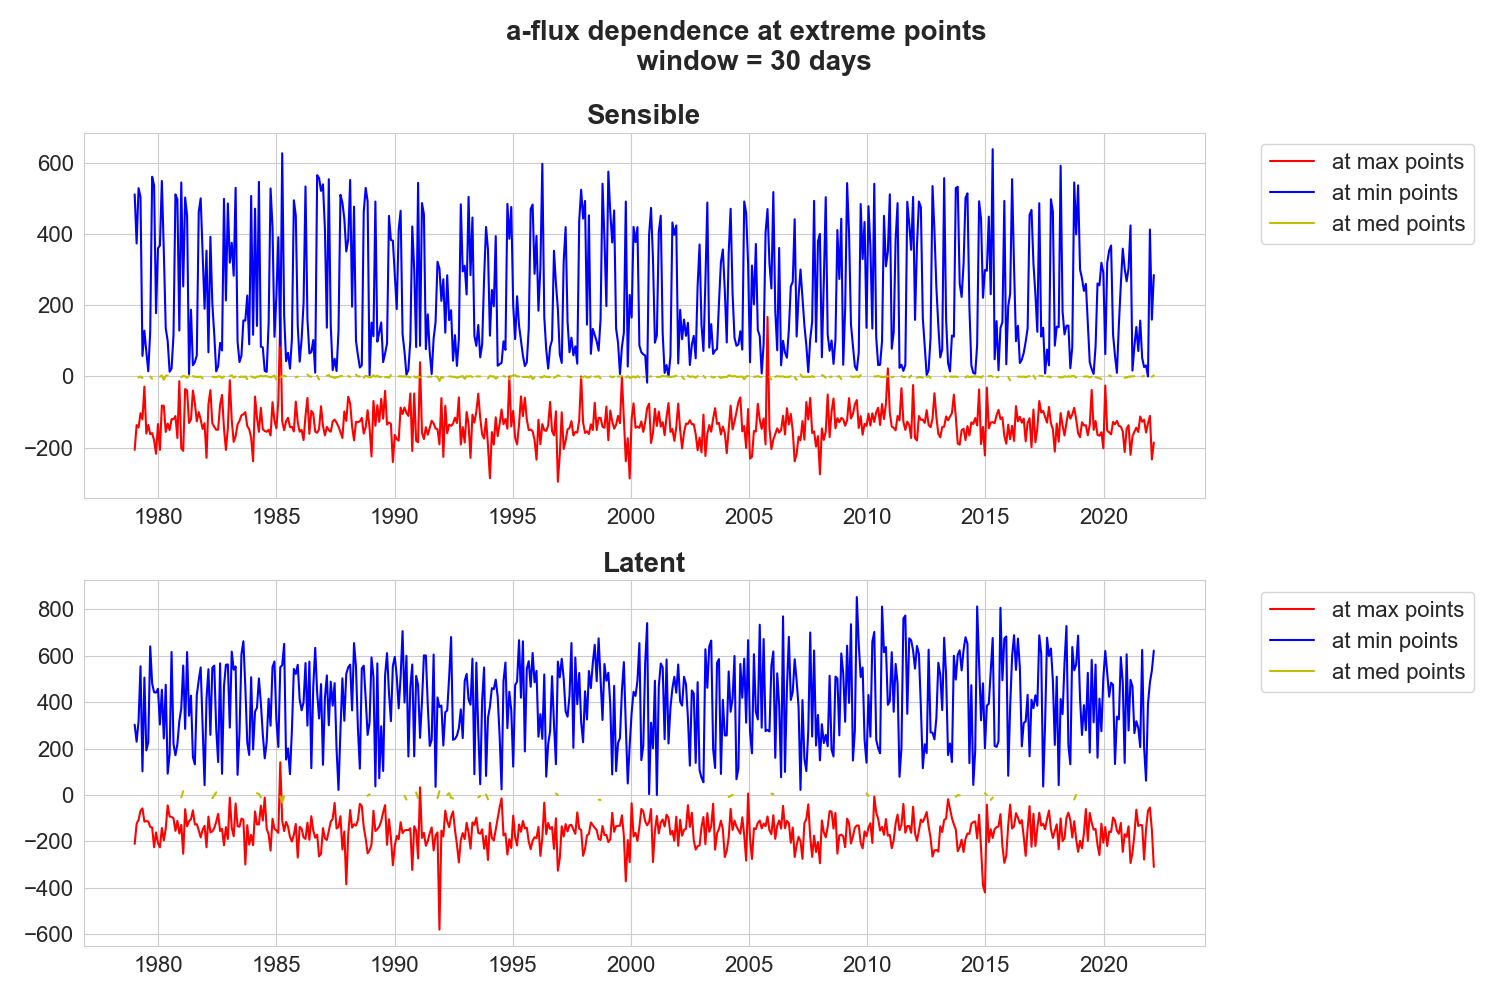
\includegraphics[width=\textwidth]{a_flux(1-15797)_30}
	\caption{Поведение оценок коэффициента $a$ в точках экстремальных значений потоков в течение $1979$--$2021$~гг. с шагом в $30$ дней}
	\label{fig_a_flux_month}
\end{figure}

\begin{figure}[!h]
	\centering
	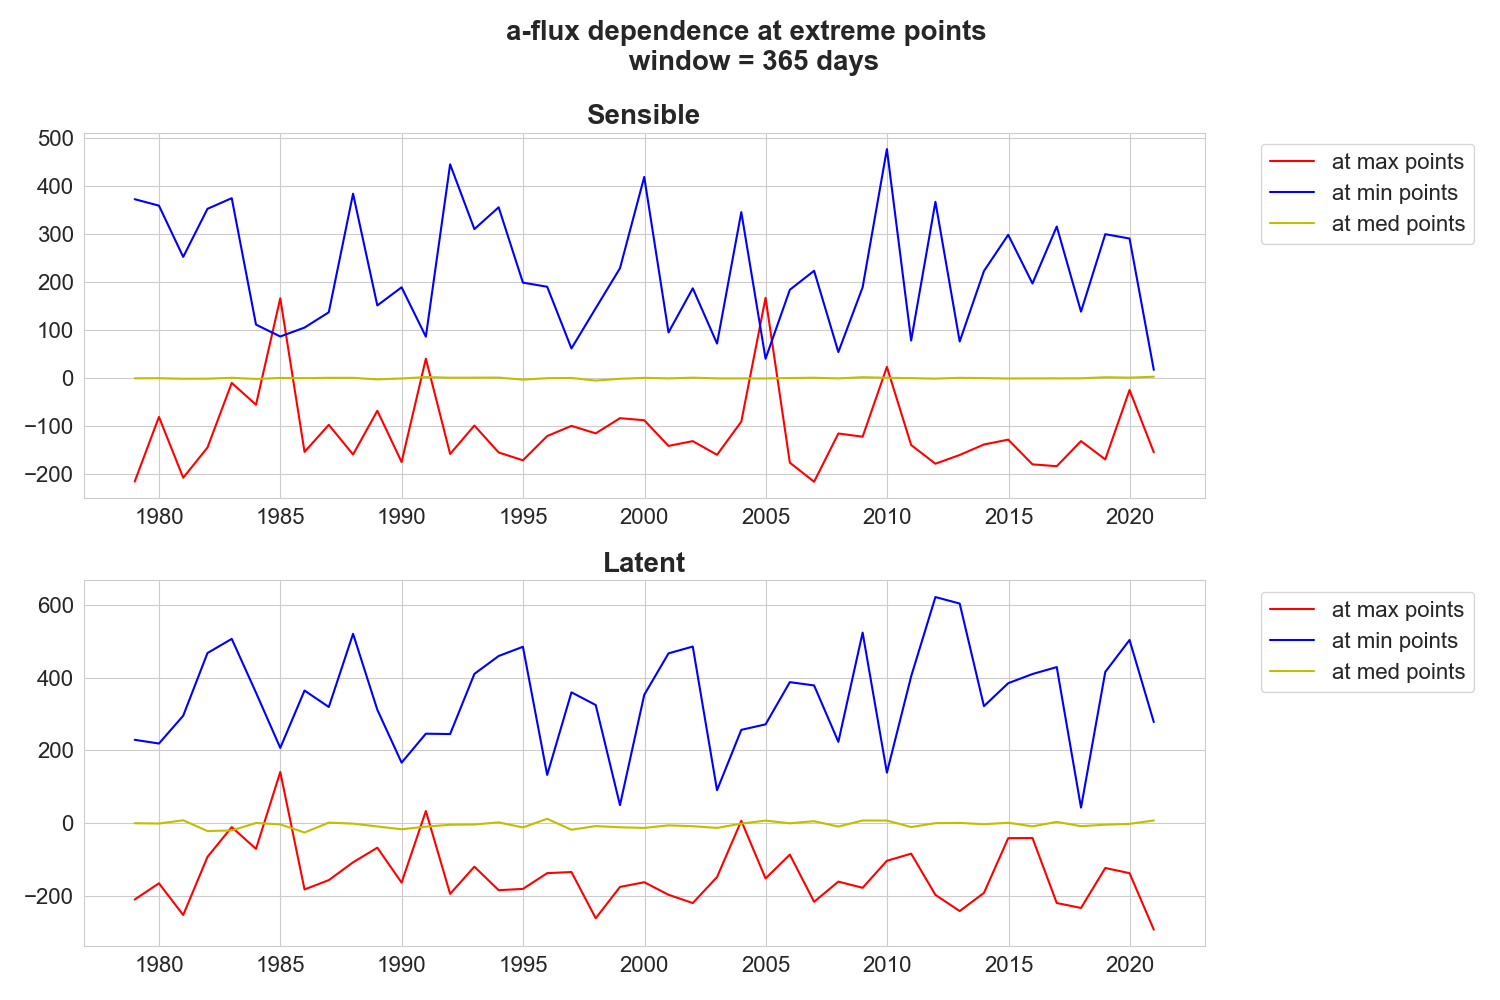
\includegraphics[width=\textwidth]{a_flux(1-15797)_365}
	\caption{Поведение оценок коэффициента $a$ в точках экстремальных значений потоков в течение $1979$--$2021$~гг. с шагом в $365$ дней}\label{fig_a_flux_year}
\end{figure}

\section{Разложение Карунена-Лоэва}
\subsection{Результаты}
\label{analysis}
В этом разделе представлены результаты применения методологии, описанной в разделе~\ref{Methodology}, к данным пространственно-временного реанализа ERA5.


\subsection{Описание данных и тренды}
Исследование основано на данных реанализа ERA5, которые включают в себя температуру поверхности океана, общий тепловой поток (сумму видимых и скрытых потоков) и приземное давление в Северной Атлантике за период с $1$ января $1979$ года по $31$ декабря $2024$ года. Данные сосредоточены в узлах однородной сетки с шагом в $0,5$ градуса, охватывающей Северную Атлантику. Границы сетки по широте варьируются от $-90$ до $0$ градусов, а по долготе - от $0$ до $80$ градусов. Временной интервал между двумя последовательными измерениями составляет $6$ часов, в день проводятся $4$ измерения: в полночь, $06:00$, $12:00$ и в $18:00$.

На рисунке~\ref{data_example} показан пример визуализации данных с ежедневным усреднением: картинка слева соответствует суммарному тепловому потоку, в середине - температуре поверхности океана, а справа -- атмосферному давлению. Цветовая шкала на левом графике меняется с синего (при отрицательных значениях) до белого (при значениях, близких к нулю), а затем до красного (при положительных значениях). Яркость цвета в определенной точке соответствует удаленности модуля значения от нуля. Для среднего и правого графиков, очевидно, значения могут быть только положительными, поэтому их шкала значений варьируется от белого (при значениях, близких к нулю) до ярко-красного. Светло-зеленый цвет обозначает участки суши.


\begin{figure}
	\center{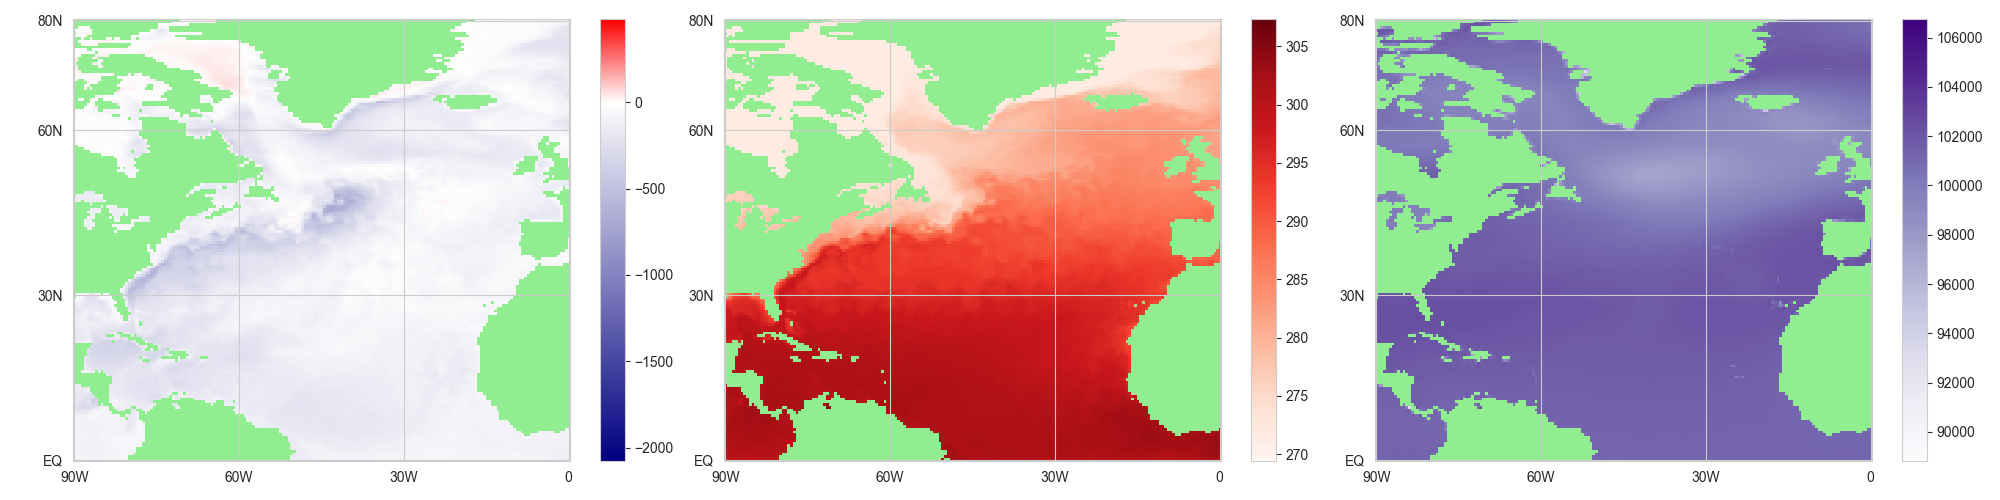
\includegraphics[width=\textwidth]{16436.png}}
	\caption{Пример используемых данных: суммарный тепловой поток, SST и атмосферное давление, усредненные данные за $1$ января $2024$ года}
	\label{data_example}
\end{figure}

Три рассмотренные переменные сильно коррелируют друг с другом, что видно из их попарных корреляций. Пример корреляций за $7$ дней показан на рисунке~\ref{correlations}. В то же время нельзя говорить о существовании какого-то одного типа зависимости: скорее, выделяются определенные области или зоны с положительными или отрицательными корреляциями.

\begin{figure}
	\center{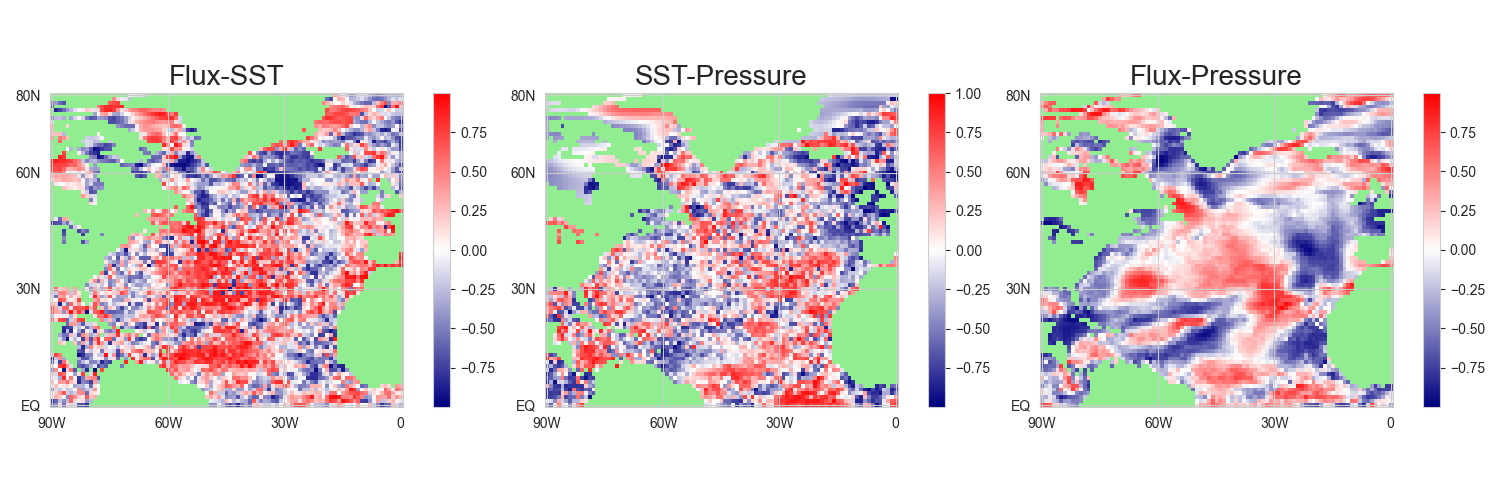
\includegraphics[width=\textwidth]{Correlations.png}}
	\caption{Попарные корреляции суммарного теплового потока, SST и атмосферного давления за период $01.01.2024-08.01.2024$}
	\label{correlations}
\end{figure}

В этом разделе также описывается временная изменчивость каждой из рассматриваемых переменных с $1979$ по $2024$ год. В статье~\cite{gorshenin2023stochastic} была рассмотрена временная изменчивость явных и скрытых тепловых потоков за практически тот же временной период. В этой работе мы исследуем суммарный поток (сумму явных и скрытых тепловых потоков в каждой точке сетки), температуру поверхности океана и атмосферное давление. В качестве средних значений они могут рассматриваться независимо в каждой точке.

\begin{figure}
	\center{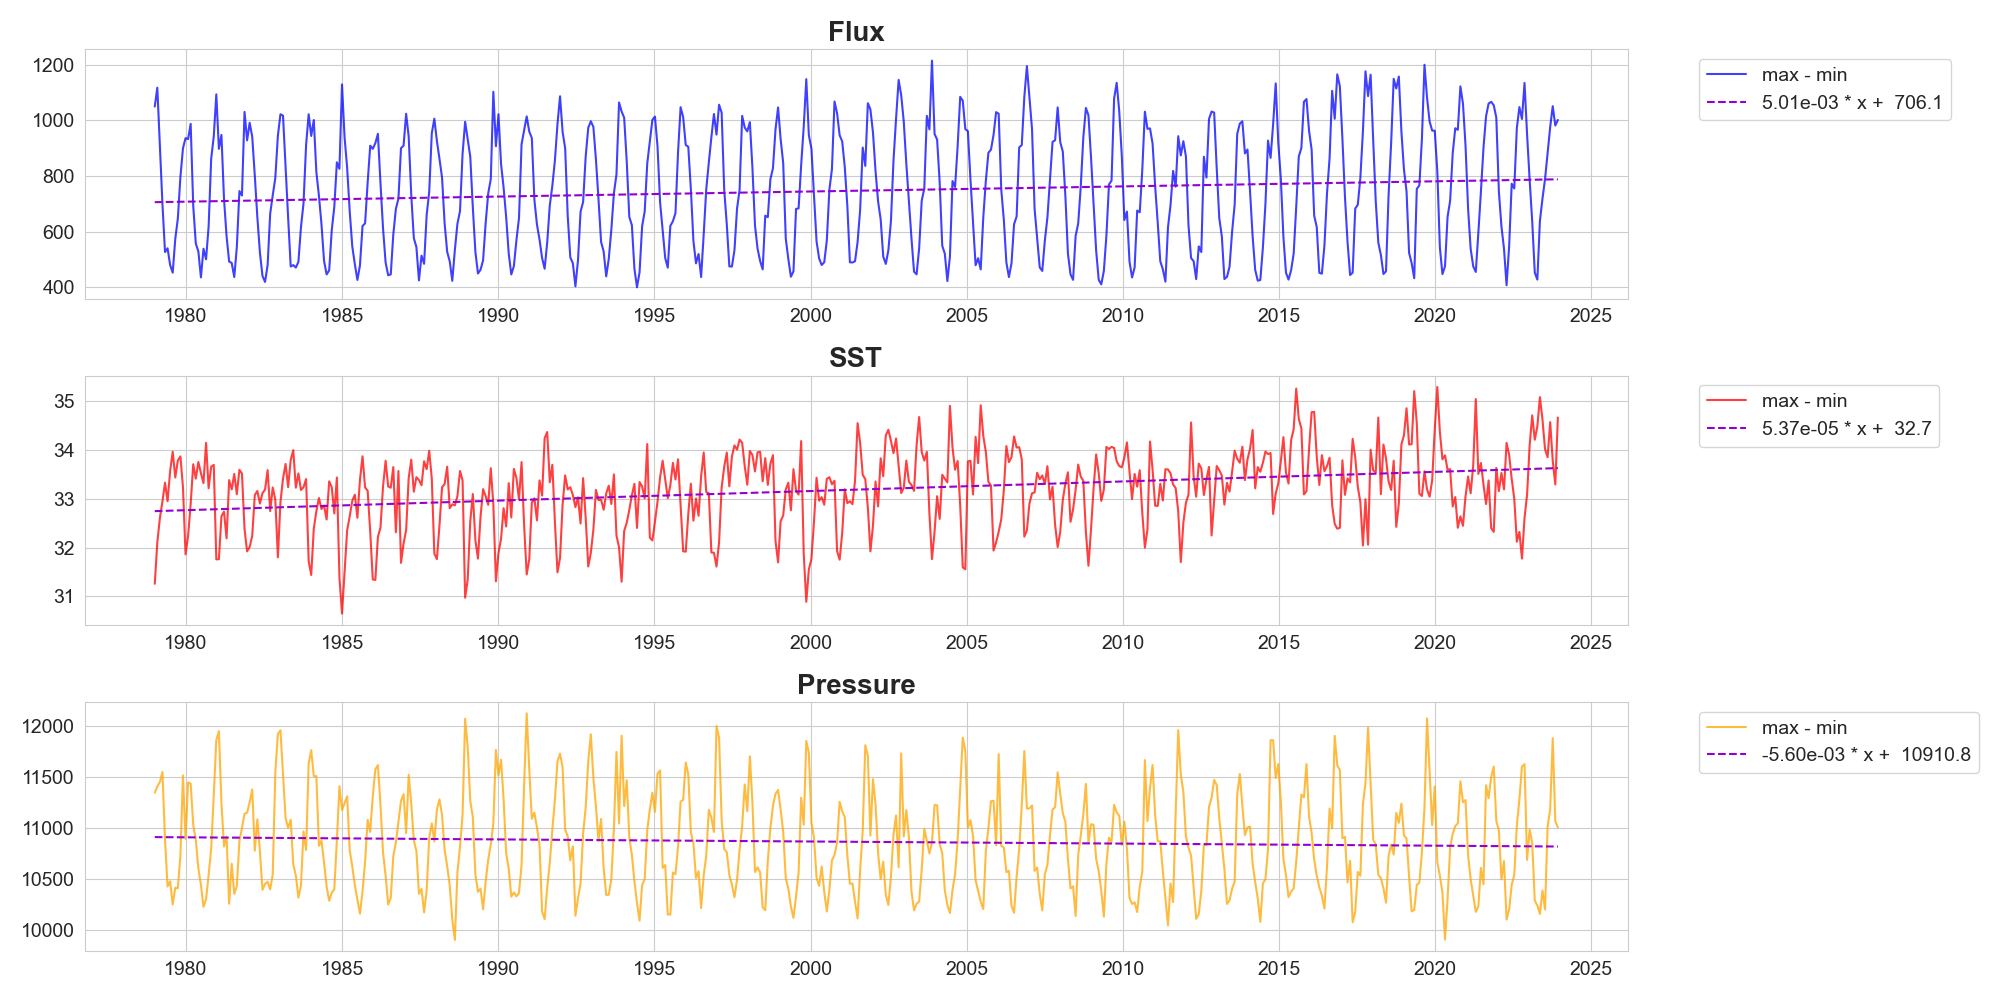
\includegraphics[width=1.0\textwidth]{difference_max-min_raw_(0-16554)_30.png}}
	\center{a)}
	\center{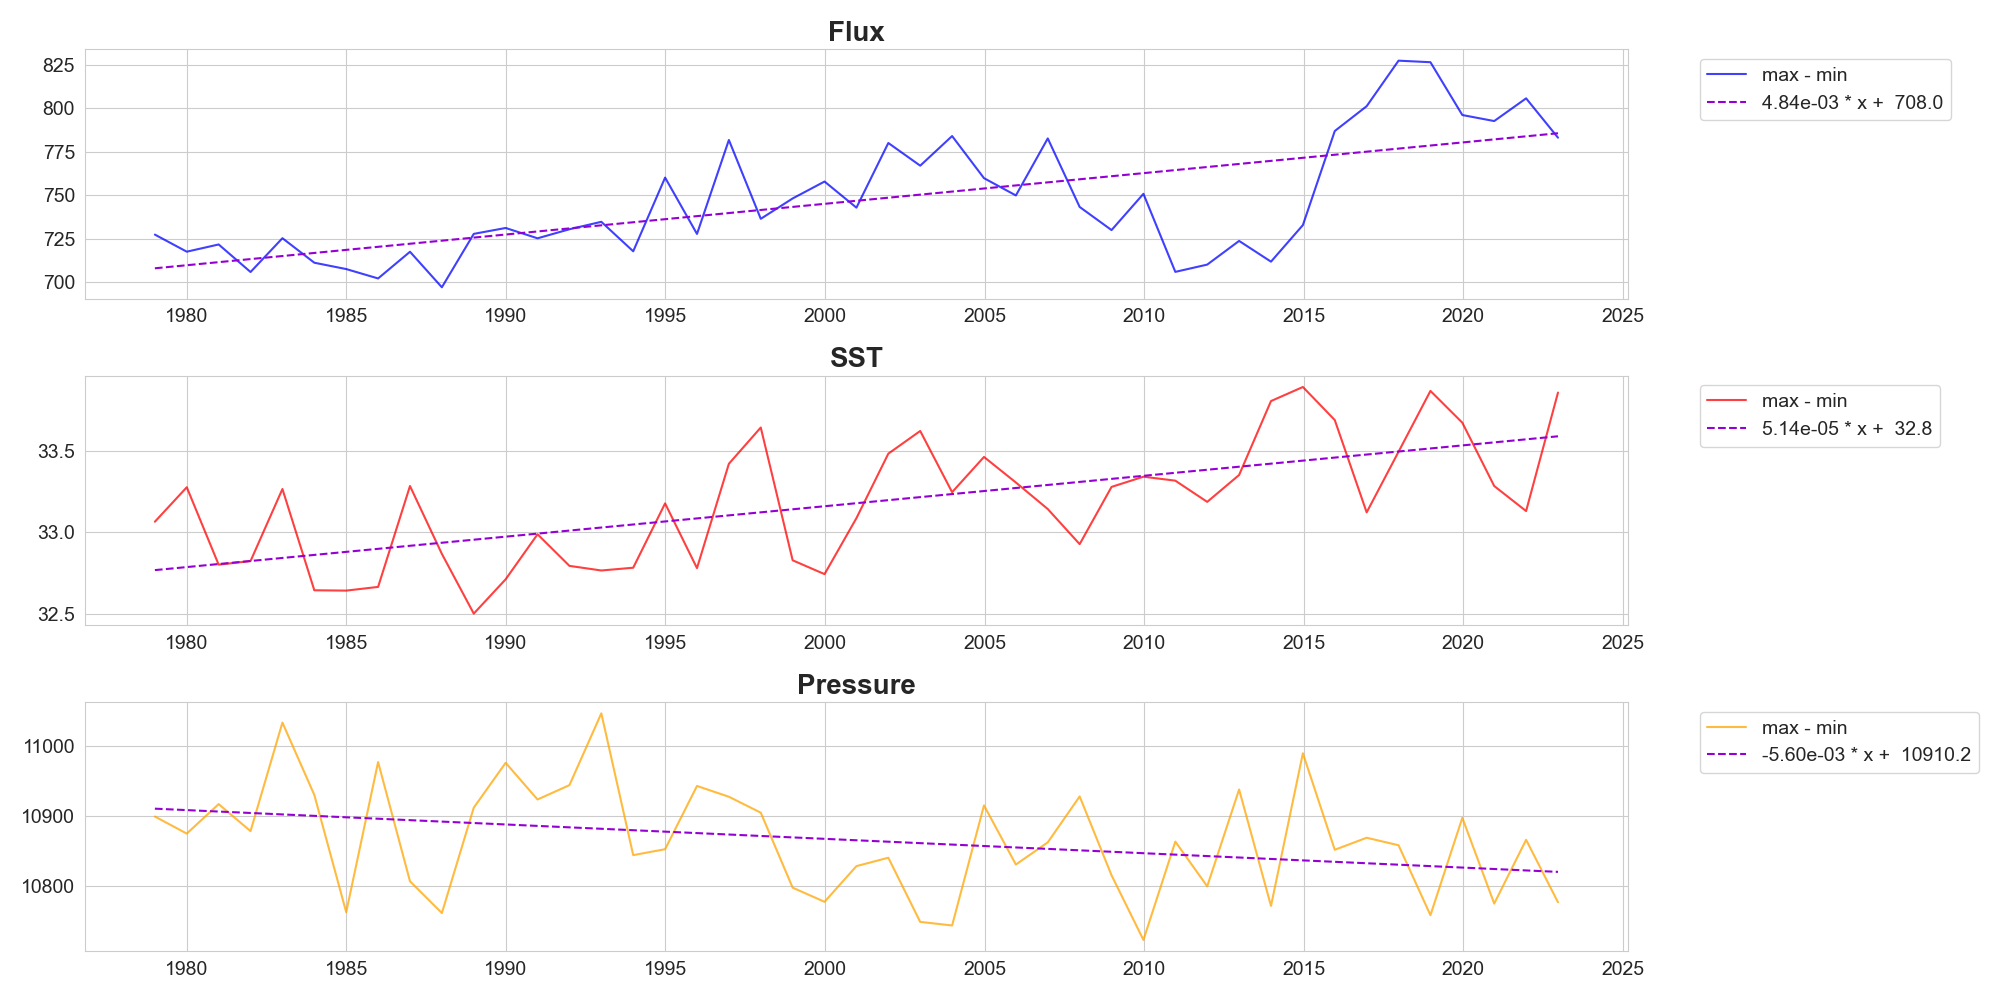
\includegraphics[width=1.0\textwidth]{difference_max-min_raw_(0-16554)_365.png}}
	\center{б)}
	\caption{Разница между максимумом и минимумом по всей рассматриваемой области данных суммарного потока, SST и давления за $1979--2023$ годы при усреднении по окну шириной а) $30$ и б)$365$ дней}
	\label{raw_trends}
\end{figure}

На рисунке~\ref{a_extreme_365} представлены максимальное, среднее и минимальное значения построенных точечных оценок коэффициента $a$ по формуле~\eqref{Ito} для временного ряда совокупного теплового потока, усредненного за годичный период. Хорошо виден ярко выраженный положительный линейный тренд для максимальных значений потока и SST (красная кривая) и незначительный значительный отрицательный тренд для минимальных значений (синяя кривая), причем для SST он выражен сильнее, чем для потоков. Средние значения не имеют выраженного тренда за весь рассматриваемый период (зеленая кривая). Также можно наблюдать почти двухлетний цикл, но он, по-видимому, не является статистически значимым. Длительные циклы слегка заметны, но не подтверждены. Для атмосферного давления тенденция прямо противоположная. Виден относительно сильный отрицательный тренд для максимальных значений и слабый положительный тренд для минимальных значений (красная и синяя кривые соответственно). Что касается значений SST, то для средних значений тренд вообще отсутствует (зеленая кривая).


\begin{figure}
	\center{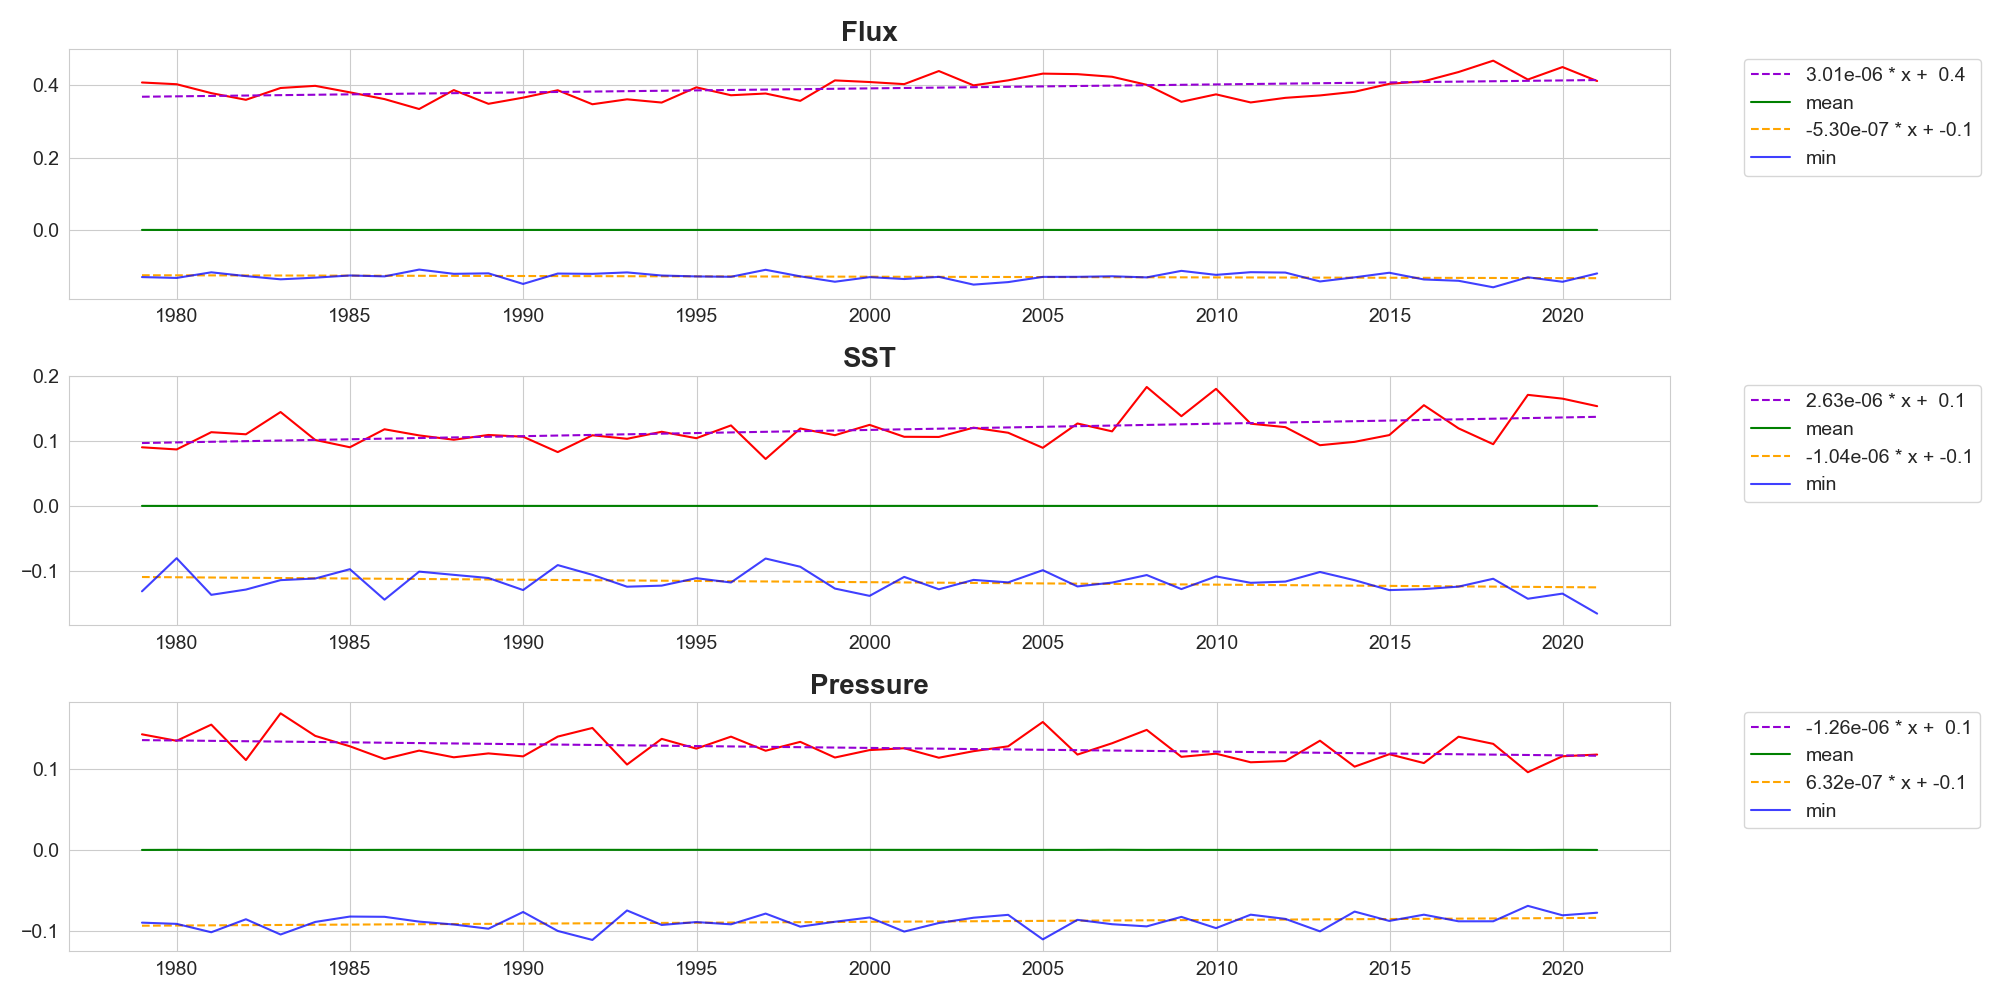
\includegraphics[width=1.0\textwidth]{a_(1-16071)_365_fit_regression.png}}
	\caption{Динамика максимального, минимального и среднего значений оценок, полученных для коэффициента $a(X,t)$ для потока, SST и давления за период 1979-2024 гг.} 
	\label{a_extreme_365}
\end{figure}

В таблице~\ref{table_angular_3d} представлены угловые коэффициенты для линейных трендов и приращения для максимальных и минимальных оценок коэффициентов дрейфа $A$ с ежемесячным и годовым усреднением.

\begin{table}
	\caption{Угловые коэффициенты линейного тренда для максимальной и минимальной оценок коэффициента сноса $a$ с различными масштабами усреднения \label{table_angular_3d}}
	\centering
	\begin{tabular}{|c|c|c|c|c|c|c|}
		\hline
		Переменная & Усреднение, дни & $k$ для максимума & прирост максимума & $k$ для минимума & прирост для минимума\\
		\hline
		Суммарный поток & $30$ & $2.86 \cdot 10^{-6}$ & $4.59 \cdot 10^{-2}$ & $-4.44 \cdot 10^{-7}$ & $-7.13 \cdot 10^{-3}$ \\
		Суммарный поток & $365$ & $3.01 \cdot 10^{-6}$ & $4.85 \cdot 10^{-2}$ & $-5.30 \cdot 10^{-7}$ & $-8.52 \cdot 10^{-3}$    \\
		SST & $30$ & $2.71 \cdot 10^{-6}$ & $4.35 \cdot 10^{-2}$ & $-1.21 \cdot 10^{-6}$ & $-1.95 \cdot 10^{-2}$   \\
		SST & $365$ & $2.63 \cdot 10^{-6}$ & $4.23 \cdot 10^{-2}$ & $-1.04 \cdot 10^{-6}$ & $-1.67 \cdot 10^{-2}$    \\
		Давление & $30$ & $-1.30 \cdot 10^{-6}$ & $-2.10 \cdot 10^{-2}$ & $7.29 \cdot 10^{-7}$ & $1.17 \cdot 10^{-2}$ \\
		Давление & $365$ & $-1.26 \cdot 10^{-6}$ & $-2.03 \cdot 10^{-2}$ & $6.32 \cdot 10^{-7}$ & $1.01 \cdot 10^{-2}$ \\
		\hline
	\end{tabular}
\end{table}


\subsection{Собственные векторы}
На рисунках ~\ref{SST-SST_trends}--~\ref{Flux-SST_trends} показана эволюция экстремальных характеристик (максимума, минимума и среднего значения) для первого собственного вектора из упорядоченного набора для пар SST-SST и Flux-SST, соответственно, и соответствующие линии линейной регрессии, где переменной Flux обозначается суммарный тепловой поток, а упорядочивание происходит по убыванию модулей соответствующих собственных значений. Для всех этих временных рядов практически нет тренда, поскольку угловые коэффициенты оценочной регрессии имеют порядок от $10^{-8}$ до $10^{-6}$ и кажутся слишком малыми по сравнению с масштабом ряда, чтобы считаться значимыми. Следует отметить, что для минимальных значений SST наблюдается заметно больший диапазон колебаний от года к году. Для пары Flux-Flux картина аналогична паре SST-SST, но амплитуда годового хода значительно меньше.

\begin{figure}
	\center{\includegraphics[width=1.0\textwidth]{SST-SST_(0-16554)_mean_30_fit_regression.png}}
	\caption{Экстремальные значения и их тренды для первого собственного значения из упорядоченного набора для пары SST-SST за $1979--2024$ годы с усреднением в $30$ дней}
	\label{SST-SST_trends}
\end{figure}

\begin{figure}
	\center{\includegraphics[width=1.0\textwidth]{Flux-SST_(0-16554)_mean_30_fit_regression.png}}
	\caption{Экстремальные значения и их тренды для первого собственного значения из упорядоченного набора для пары Flux-SST за $1979--2024$ годы с усреднением в $30$ дней}
	\label{Flux-SST_trends}
\end{figure}

На рисунке~\ref{Векторы потока-Flux_eigenvectors} хорошо виден волновой и динамический перенос тепла вдоль атлантической меридиональной циркуляционной системы. Волна жары, фронт которой проходит от побережья Северной Америки до Африки, двигаясь с юга на север, захватывается системой течений вдоль Атлантического побережья (Гольфстрим и Североатлантическое течение) и затухает в северо-восточном направлении.

С помощью этих данных можно количественно оценить энергию волны и скорость ее рассеяния. Следующие два собственных вектора из упорядоченного набора имеют значения, близкие друг к другу, и на $10$ порядков меньше, чем первый собственный вектор. Структуры этих векторов похожи друг на друга и, как правило, повторяют первый собственный вектор. При визуализации собственных векторов используется цветовая шкала, аналогичная SST и давлению, показанным на рисунке ~\ref{data_example}: цвет меняется с белого при значениях, близких к нулю, а затем на темно-синий при увеличении значений. Яркость цвета в определенной точке соответствует расстоянию значения от нуля. Светло-зеленый цветом показаны участки суши.

Собственные векторы матрицы SST (см. рисунок ~\ref{SST-SST_eigenvectors}) аналогичны собственным векторам матрицы Flux, но имеют заметные отличия. Перенос тепла с юга на север происходит в основном в виде крупномасштабных вихрей, которые перемещаются вдоль системы течений и ослабевают в районах Исландского минимума и к югу от Азорских островов. Здесь различия первого собственного вектора в терминах собственных значений имеют тот же порядок, что и для SST, однако структурно второй и третий собственные векторы, по-видимому, отстают по отношению к основному собственному вектору. Также можно оценить общую энергию этих потоков как сумму квадратов собственных значений матрицы диффузии.


Пара давление-давление (см. рисунок~\ref{press-press_eigenvectors}) демонстрирует создание и динамику крупномасштабных структур в Северной Атлантике. Кольца давления проходят через весь Атлантический регион, в основном концентрируясь в северной части вблизи Исландской минимальной зоны и энергетической зоны Лабрадора. Для первого сильно доминирующего собственного вектора динамика в основном наблюдается вдоль Гольфстрима в направлении Североатлантической Исландской минимальной зоны, но для второго и третьего собственных векторов (которые значительно меньше по абсолютным значениям) мы наблюдаем более сложную динамику.

\begin{table}
	\caption{Угловые коэффициенты линейного тренда для собственных значений с различными масштабами усреднения \label{table_angular_eigens}}
	\centering
	\begin{tabular}{|c|c|c|}
		\hline
		Пара & $k$ для усреднения в $30$ дней & $k$ для усреднения в $365$ дней\\
		\hline
		Flux-Flux & $-1.87 \cdot 10^{4}$ & $-5.26 \cdot 10^{3}$ \\
		SST-SST & $1.32 \cdot 10^{1}$ & $1.31 \cdot 10^{1}$ \\
		Давление-давление & $1.31 \cdot 10^{6}$ & $1.73 \cdot 10^{6}$ \\
		Flux-SST & $2.95 \cdot 10^{2}$ & $2.96 \cdot 10^{2}$ \\
		SST-давление & $2.34 \cdot 10^{3}$ & $2.33 \cdot 10^{3}$ \\
		Flux-давление & $-2.10 \cdot 10^{4}$ & $3.59 \cdot 10^{4}$ \\
		\hline
	\end{tabular}
\end{table}

На рисунках~\ref{eigenvalues_mean_30} и ~\ref{eigenvalues_mean_365} показана эволюция первых собственных значений из упорядоченного набора (отсортированных по убыванию их абсолютных значений) с усреднением по окну шириной в $30$ и $365$ дней, соответственно, а также соответствующие линейные тренды. Таблица~\ref{table_angular_eigens} показывает угловые коэффициенты трендов для обоих масштабов усреднения.


\begin{figure}
	\center{\includegraphics[width=\textwidth]{(0-16767)_mean_30_fit_regression_eigenvalues.png}}
	\caption{Первые собственные значения упорядоченного набора для каждой пары переменных, усредненные за $30$ дней и их линейные тренды}
	\label{eigenvalues_mean_30}
\end{figure}

\begin{figure}
	\center{\includegraphics[width=\textwidth]{(0-16767)_mean_365_fit_regression_eigenvalues.png}}
	\caption{Первые собственные значения упорядоченного набора для каждой пары переменных, усредненные за $365$ дней и их линейные тренды}
	\label{eigenvalues_mean_365}
\end{figure}

\begin{figure}
	\center{\includegraphics[width=\textwidth]{flux-flux_eigenvectors.png}}
	\caption{Первые три собственных вектора из упорядоченного набора для пары Поток-поток за $01.01.23$, $01.04.23$, $01.07.23$ и $01.10.23$}
	\label{Flux-Flux_eigenvectors}
\end{figure}

\begin{figure}
	\center{\includegraphics[width=\textwidth]{sst-sst_eigenvectors.png}}
	\caption{Первые три собственных вектора из упорядоченного набора для пары SST-SST за $01.01.23$, $01.04.23$, $01.07.23$ и $01.10.23$}
	\label{SST-SST_eigenvectors}
\end{figure}

\begin{figure}
	\center{\includegraphics[width=\textwidth]{press-press_eigenvectors.png}}
	\caption{Первые три собственных вектора из упорядоченного набора для пары Давление-Давление за $01.01.23$, $01.04.23$, $01.07.23$ и $01.10.23$}
	\label{press-press_eigenvectors}
\end{figure}

\subsection{Взаимосвязь между потоком, SST и давлением}
В этом разделе рассматривается взаимосвязь между изучаемыми характеристиками с помощью их совместных диффузионных матриц. Построение совместных матриц описано в разделе~\ref{algorithm}. Взаимодействие между парами в течение года для первых трех собственных векторов в упорядоченном наборе показано на $4 \cdot 3$ рисунках для каждой пары в разные сезоны: за $01.01.23$, $01.04.23$, $01.07.23$, $01.10.23$. Динамика суммарного потока и SST отчетливо видна на рисунке~\ref{Flux-SST_eigenvectors}. В то же время, при основном значении порядка $2*107$ градусов $\cdot Вт/м^2$, перенос теплового взаимодействия с юга на север происходит аналогично динамике SST, но с заметным влиянием тепловых потоков в Северной Атлантике. Для второго и третьего собственных векторов, значения которых имеют порядок $10^{-1}$ градусов $\cdot W/m^2$, динамика выглядит более интересной, теплопередача происходит как адвективно, так и волнообразно вдоль границы раздела океан-суша.

Собственные векторы матрицы Поток-давление представляют собой очень интересную структуру (см. рисунок~\ref{Flux-press_eigenvectors}). Динамическое взаимодействие осуществляется в виде преимущественно кольцевых структур, которые выражают крупномасштабную динамику атмосферы (циклоны), связанную с тепловыми потоками. Здесь, как и на предыдущих рисунках, обертоны (второй и третий собственные вектора) выглядят насыщеннее, чем первый, который несет основную энергию, но значимость обертонов довольно велика, порядка $5*102$ $\cdot Вт/м^2$. Структурно видна взаимосвязь с зонами низкого и высокого давления в Северной Атлантике: противофазный максимум первого вектора проявляется в южных широтах, минимум - в северных, и наоборот для второго и третьего векторов.

\begin{figure}
	\center{\includegraphics[width=\textwidth]{flux-sst_eigenvectors.png}}
	\caption{Первые три собственных вектора из упорядоченного набора для пары Flux-SST за $01.01.23$, $01.04.23$, $01.07.23$ и $01.10.23$}
	\label{Flux-SST_eigenvectors}
\end{figure}

\begin{figure}
	\center{\includegraphics[width=\textwidth]{flux-press_eigenvectors.png}}
	\caption{Первые три собственных вектора из упорядоченного набора для пары Flux-Давление за $01.01.23$, $01.04.23$, $01.07.23$ и $01.10.23$}
	\label{Flux-press_eigenvectors}
\end{figure}



           % Глава 2
\chapter{Программный комплекс}
\label{ch:Algorithms}
В данной главе обсуждаются вопросы программной реализации описанных в предыдущих разделах методов с использованием высокопроизводительных вычислений для анализа пространственно-временных данных реанализа.
\section{Непараметрический метод}
 На рисунке~\ref{fig:algo_nonparametric} приведена блок-схема алгоритма непараметрического статистического оценивания~\ref{sec:Nonparametic} коэффициентов $a(t,x)$ и $b(t,x)$ СДУ  Ито~\eqref{eq:Ito}. Величины $t_0$ и $t_1$ соответствуют подряд идущим моментам времени. 

\begin{figure}[!h]
	\centering
	\includegraphics[width=\textwidth]{diagram_eng}
	\caption{Блок-схема непараметрического алгоритма расчета оценок для коэффициентов $a$ и $b$} \label{fig:algo_nonparametric}
\end{figure}

Оценим вычислительную сложность этого алгоритма. Поскольку на каждом шаге $t \in [t_0,T]$ рассматриваются два момента времени $t_1$ и $t_2$, в которых присутствует вложенный цикл по уникальным значениям двух двумерных массивов, являющихся рассматриваемой сеткой, то сложность алгоритма будет составлять $O(t\times n^2)$, где $n$ – число элементов каждого из массивов. C учетом размеров рассматриваемой сетки, в текущей работе значения этих параметров следующие: $n=161\times181=29141$, $t = [0, 15917]$ - количество дней за рассматриваемый промежуток времени.

Расчет оценок коэффициентов $a$ и $b$, их корреляции и отношение $F$ выполнялись на высокопроизводительном кластере в индивидуальной вычислительной среде на основе технологии виртуальной контейнеризации Docker~\cite{peinl2016docker}. После выполнения всех расчетов для рассматриваемых величин были на локальной машине отрисованы графики в формате карт с последующей сборкой в видеофайлы формата mp4 продолжительностью около часа каждое.  
Программная реализация была выполнена на языке Python 3.7 с использованием библиотек Matplotlib, NumPy, Pandas, SciPy, Skimage, Seaborn, Xarray (для чтения grib-файлов) и др.

Исходные данные измерений явного и скрытого потока представляли собой 2 файла формата grib из открытой базы ERA5\footnote{https://www.ecmwf.int/en/forecasts/datasets/reanalysis-datasets/era5}, каждый из которых содержал в себе ежедневные измерения с шагом в $6$ часов за период 01.01.1979 -- 31.07.2022 на сетке с шагом в $0.5$ градуса со значениями широты в пределах $[-90, 0]$ и долготы в интервале $[0, 80]$ градусов. Для расчета коэффициентов данные были перегруппированы в numpy-массивы по десятилетиям (1979-1989гг., 1989-1999гг., 1999-2009гг., 2009-2019гг., 2019-2022гг.) с уменьшением размерности сетки до 1 градуса. Затем для выполнения расчетов с шагом в $1$ день данные были усреднены по $4$ подряд идущих измерения, за каждый день. Для выполнения расчетов оценок коэффициентов $a$ и $b$ данные предварительно дополнительно подвергались дискретизации, как подробно описано в разделе~\ref{sec:Disctretization}. Благодаря свойствам марковости рассматриваемых процессов стало возможно реализовать параллельный расчет на нескольких процессах-нитях с последующей сборкой результатов и обработкой границ интервалов родительским процессом, где параллелизм выполнялся по координате времени. 

Программы оценивания эволюции параметров динамико-стохастической модели потоков тепла между океаном и атмосферой а также визуализации результатов были зарегистрированы в Роспатенте~\cite{progbib1, progbib2}.

%\clearpage

\section{Полупараметрический метод}
\label{sec:AlgoSemiparametric}
В данном разделе представлена блок-схема полупараметрического алгоритма оценивания случайных коэффициентов $a$ и $b$ СДУ Ито~\eqref{eq:Ito}.
\begin{figure}
	\centering
	\includegraphics[width=\textwidth]{semiparametric.png}
	\caption{Блок-схема полупараметрического алгоритма расчета оценок для коэффициентов $a$ и $b$}
	\label{fig:SemiparametricAlgo}
\end{figure}

\subsection{Выделение компонент связности}
\label{sec:ComponentsAlgo}
В данном разделе представлен псевдокод алгоритма выделения эволюции компонент, описанного в разделе~\ref{sec:Components}.
\begin{algorithm}[!h]
	\caption{Динамическое определение числа локальных компонент}
	\label{AlgGreedy}
	\begin{algorithmic}[1]
		\Function{NumGreedy}{Params, $ I^{(n)}$, $J^{(n+1)}$}
		\State  $I_0\gets \emptyset$, $J_0\gets \emptyset$, Comps$\gets \emptyset$;\Comment{{\em Инициализация}}
		\Repeat \Comment{{\em Продолжающиеся или новые компоненты}}
		\State \LongComment{{\em Оптимизация выражения~\eqref{I} с учетом условия~\eqref{Dist}}}
		\State [I, J]$\gets$\Call{FindI}{Params, $J^{(n+1)}\setminus J_0$, $I^{(n)}\setminus I_0$};
		\If{I $\neq \emptyset$}\Comment{{\em Найдена предшествующая $J$ компонента}}	
		\State $I_0\gets I_0\cup I$, $J_0\gets J_0\cup J$;
		\Else\Comment{{\em Добавление новой компоненты}}
		\State $J_0\gets J_0\cup J$;
		\State Comps $\gets$ \Call{AddNewComp}{Params, J};
		\EndIf
		\Until{($J^{(n+1)}\setminus J_0 \neq \emptyset$)}
		\State \Return Comps;
		\EndFunction
	\end{algorithmic}
\end{algorithm}

Предполагается, что данный алгоритм применяется для компонент с положительными весами (нулевые значения соответствуют случаю уменьшению их числа на каком-либо шаге). Кроме того, для всех допустимых значений $i\neq j$ и $n$ должны существовать такие $\delta_a>0$ и $\delta_\sigma>0$, что выполнено хотя бы одно из условий $\left|a_i^{(n)}-a_j^{(n)}\right|>\delta_a$, $\left|\sigma_i^{(n)}-\sigma_j^{(n)}\right|>\delta_\sigma$. Если же они оба нарушены, то необходимо объединять эти компоненты в одну с соответствующей корректировкой (суммированием) весов. То есть предполагается, что все компоненты различны, -- это гарантирует корректность применения жадного алгоритма.

Алгоритм~\ref{AlgGreedy} используется в качестве важной составной части  метода формирования матрицы связности. Она представляет собой вспомогательную структуру, в которую на каждом шаге скользящего окна сохраняется актуальное состояние всех выделенных к текущему моменту компонент. Сначала ко всему ряду применяется метод EM-типа для определения числа компонент на каждом шаге (как было отмечено выше, оно не может убывать). Затем в двухмерном пространстве $(a, \boldsymbol \sigma)$ используется один из методов кластеризации с полученным жадным алгоритмом числом локальных компонент-кластеров. Веса не учитываются, так как вклад компоненты в смесь может изменяться, при этом параметры -- математическое ожидание и дисперсия -- варьируются не слишком сильно и тогда считается, что это та же самая компонента. Соответствующая процедура представлена в алгоритме~\ref{AlgConnect}.

\begin{algorithm}[!h]
	\caption{Определение компонент связности в СРС-методе}
	\label{AlgConnect}
	\begin{algorithmic}[1]
		\Function {MSMComponents}{Data, options}
		\State Params $\gets$\Call{EMs}{Data, options.EM}\Comment{{\em СРС-метод}}
		\State \LongComment{{\em Инициализация числом ненулевых компонент на первом шаге}}
		\State  Comps$^{(1)}$$\gets$Params.k$^{(1)}$;
		\For{(n = 1:{length}(Params)-1)}
		\State Comps$^{(n+1)}$ $\gets$ \Call{NumGreedy}{Params, $ I^{(n)}$, $J^{(n+1)}$};
		\EndFor
		\State \LongComment{{\em Метки для каждого набора параметров, кластеризация}}
		\State Labels $\gets$ \Call{Clust}{Params, {max}(Comps), options.ClustAlg};
		\State \LongComment{{\em Матрица связности для компонент СРС-метода}}
		\State HistMatrConnect$\gets$ \Call{Сonnectivity}{Params, Labels};	
		\State \Call{PlotComp}{HistMatrConnect};\Comment{{\em Визуализация результатов}}
		\State \Return HistMatrConnect;
		\EndFunction
	\end{algorithmic}
\end{algorithm}

Очевидно, что данная процедура может быть использована и в случае смесей многомерных распределений. 
Программы с реализацией описанных алгоритмов на языке Python были зарегистрированы в системе Роспатента~\cite{progbib4, progbib5}.
%\clearpage

\section{Разложение Карунена-Лоэва}
\label{sec:AlgoKarhunen}
На рисунке \ref{fig:KarhunenAlgo} представлена блок-схема алгоритма разложения коэффициента диффузии на собственные вектора, описанного в разделе~\ref{sec:Karhunen}.
\begin{figure}
	\centering
	\includegraphics[width=\textwidth]{decomposition_concept.png}
	\caption{Блок-схема алгоритма разложения коэффициента диффузии}
	\label{fig:KarhunenAlgo}
\end{figure}



\section{Архитектура программного комплекса}
В этом разделе описана архитектура используемого программного комплекса.


\begin{figure}[!h]
	\centering
	\includegraphics[width=0.99\textwidth]{scheme}
	\caption{Логическое представление архитектуры программного комплекса}\label{fig:app_scheme}
\end{figure}


На рисунке~\ref{fig:app_scheme} схематично показаны основные структурные компоненты проекта:
\begin{itemize}
	\item Блок \verb"Data prepocessing" содержит программные преобразование формата \verb"GRIB" (используется для хранения и передачи метеорологических данных с привязкой к сетке на двумерной географической карте) в тип данных \verb"NumPy", дискретизация (см. формулы~\eqref{eq:p_formula}--\eqref{eq:b_formula} и соответствующие пояснения к ним в разделе~\ref{sec:Nonparametic}).
	\item В блоке \verb"Docker" реализованы вычислительные алгоритмы (см. рисунок~\ref{fig:algo_nonparametric}) для расчет оценок коэффициентов $a$ и $b$, их корреляции и отношения $F$. Используется высокопроизводительный кластер архитектуры Intel x86\_64 (9 узлов на основе серверной платформы \verb"Huawei Server XH620": два \verb"Intel Xeon CPU E5-2683 v4" (2.1 GHz, 16 Core), 512 Gb RAM, 2*10G Ethernet, 2*16G \verb"FibreChannel") и индивидуальная облачная вычислительная среда на основе технологии виртуальной контейнеризации~\cite{peinl2016docker}.
	\item Блок \verb"Visualisation" предназначен для визуализации результатов: для рассматриваемых величин были на локальной машине отрисованы графики в формате карт с последующей сборкой в видеофайлы формата \verb"MP4" продолжительностью около часа каждое.
\end{itemize}

Для программной реализации использованы язык \verb"Python 3.7"\ и библиотеки \verb"Matplotlib", \verb"NumPy", \verb"Pandas", \verb"SciPy", \verb"Skimage", \verb"Seaborn", \verb"Xarray" (для чтения GRIB-файлов).

%На расчет оценок коэффициентов $a$ и $b$ ушло приблизительно $1.5$ дня непрерывных расчетов на кластере (включая накладные расходы), на расчеты $C$ и $F$ -- порядка двух часов. Отрисовка карт и сборка в видео-формат заняла около $3-4$ часов.




% \subsection{Physics-informed modification of the loss function}
% \label{section_informed_methodology}


% \new{The proposed physics-informed approach involves modifying the standard loss function, that is:
	% \begin{equation*}
		%     Loss(y_{true}, y_{predict})[i] = (1-\alpha) \cdot MSE(y_{true}, y_{predict})[i] + \alpha(t) \cdot (y_{predict} - A[i] - \sum_{j=1}^3 B_{ij} e_{ij})^2,
		% \end{equation*}
	% where $i\in \{1, 2, 3\}$ represents the variable index ($0$ for cumulative flux, $1$ for SST and $2$ for pressure),
	% \begin{equation*}
		% MSE=\frac1n\sum\limits_{j=1}n \left(y_{true}-y_{predict}\right)^2 
		% \end{equation*}
	% stands for standard mean squared error, $A_[i]$ are the estimates of the drift coefficient, $B_{ij}$ and $e_{ij}$,  $j \in \{1, 2, 3\}$ are the obtained estimations of the first eigenvalues and eigenvectors from the ordered set, and $\alpha(t)$ is the weight coefficient, that can be either a kind of hyperparameter or the self-adapting~\citep{Xiang2022} part of a neural network.
	% % , vanishing with each epoch number of the additional steps $t \in \{0, 1, \dots, 10\}$:
	% % $$
	% %     \alpha(t) = 0.6 \cdot 0.9^{-t}.
	% % $$
	% This modified loss function implements a variant of stochastic regularization to prevent the model from violating predictions, allowing neural networks to adjust to SDE limitations, and this can increase forecast quality.
	% }


           % Глава 3
\include{Dissertation/conclusion}      % Заключение
\include{Dissertation/acronyms}        % Список сокращений и условных обозначений
\chapter*{Словарь терминов}             % Заголовок
\addcontentsline{toc}{chapter}{Словарь терминов}  % Добавляем его в оглавление

\textbf{SST} : Sea Surface Temperature - температура поверхности океана

\textbf{СДУ} : Стохастическое дифференциальное уравнение      % Словарь терминов
\include{Dissertation/references}      % Список литературы
\include{Dissertation/lists}           % Списки таблиц и изображений (иллюстративный материал)

\setcounter{totalchapter}{\value{chapter}} % Подсчёт количества глав

%%% Настройки для приложений
\appendix
% Оформление заголовков приложений ближе к ГОСТ:
\setlength{\midchapskip}{20pt}
\renewcommand*{\afterchapternum}{\par\nobreak\vskip \midchapskip}
\renewcommand\thechapter{\Asbuk{chapter}} % Чтобы приложения русскими буквами нумеровались



        % Приложения

\setcounter{totalappendix}{\value{chapter}} % Подсчёт количества приложений

\end{document}

%1. Модель СДУ Ито как мат модель пространственно-временных рядов
%2. Численные методы 
%3. Программный комплекс
